\documentclass[12pt,a4paper,openany]{book}
%  RASMUS  packages
\usepackage{blindtext}
\usepackage[usenames,dvipsnames,svgnames,table]{xcolor}
\usepackage{enumitem}
\usepackage{caption}
\usepackage{placeins}
\usepackage{graphicx}

\usepackage{fancybox}
\usepackage{hyperref}

\usepackage{amsmath,amsfonts,amsthm,amssymb,xcolor}
% \let\amsboldsymbol\boldsymbol % if you want to see the bad
% boldsymbol for comparison
\usepackage{bm} % fixes boldsymbol
\usepackage{nicefrac}
\usepackage{float}

% switched to algorithm2e in lecture 9
% \usepackage{algorithm} %ctan.org\pkg\algorithms
% \usepackage{algorithmic}
% \usepackage{algorithmicx}
% \usepackage[noend]{algpseudocode}

\newtheorem{theorem}{Theorem}[section]
\newtheorem{corollary}[theorem]{Corollary}
\newtheorem{lemma}[theorem]{Lemma}
\newtheorem{observation}[theorem]{Observation}
\newtheorem{proposition}[theorem]{Proposition}
\newtheorem{invariant}[theorem]{Invariant}
\newtheorem{claim}[theorem]{Claim}
\newtheorem{fact}[theorem]{Fact}
\newtheorem{assumption}[theorem]{Assumption}
\newtheorem{warning}[theorem]{Warning}
\newtheorem{conjecture}[theorem]{Conjecture}

\newtheorem{pseudotheorem}{Pseudotheorem}[section]
\newtheorem{pseudoclaim}[theorem]{Pseudoclaim}


\theoremstyle{definition}
\newtheorem{definition}[theorem]{Definition}
\newtheorem{remark}[theorem]{Remark}

\newtheorem*{theorem*}{Theorem}
\newtheorem*{corollary*}{Corollary}
\newtheorem*{conjecture*}{Conjecture}
\newtheorem*{lemma*}{Lemma}
\newtheorem*{thm*}{Theorem}
\newtheorem*{prop*}{Proposition}
\newtheorem*{obs*}{Observation}
\newtheorem*{definition*}{Definition}
\newtheorem*{example}{Example}
\newtheorem*{remark*}{Remark}
\newtheorem*{rec*}{Recommendation}

\newenvironment{fminipage}%
  {\begin{Sbox}\begin{minipage}}%
  {\end{minipage}\end{Sbox}\fbox{\TheSbox}}

\newenvironment{algbox}[0]{\vskip 0.2in
\noindent 
\begin{fminipage}{6.3in}
}{
\end{fminipage}
\vskip 0.2in
}


\let\muchl\ll

\def\pleq{\preccurlyeq}
\def\pgeq{\succcurlyeq}
\def\pge{\succ}
\def\ple{\prec}

\def\Approx#1{\approx_{#1}}

%\def\Span#1{\textbf{Span}\left(#1  \right)}
\def\bvec#1{{\mbox{\boldmath $#1$}}}


\newcommand\congestion{\mathit{cong}}

\def\prob#1#2{\mbox{Pr}_{#1}\left[ #2 \right]}
\def\pvec#1#2{\vec{\mbox{P}}^{#1}\left[ #2 \right]}
\def\expec#1#2{{\mathbb{E}}_{#1}\left[ #2 \right]}
\def\var#1{\mbox{\bf Var}\left[ #1 \right]}

\def\defeq{\stackrel{\mathrm{def}}{=}}
\def\setof#1{\left\{#1  \right\}}
\def\sizeof#1{\left|#1  \right|}


\def\trace#1{\mathrm{Tr} \left(#1 \right)}

\def\floor#1{\left\lfloor #1 \right\rfloor}
\def\ceil#1{\left\lceil #1 \right\rceil}

\def\dim#1{\mathrm{dim} (#1)}
\def\sgn#1{\mathrm{sgn} (#1)}

\def\union{\cup}
\def\intersect{\cap}
\def\Union{\bigcup}
\def\Intersect{\bigcap}

\def\abs#1{\left|#1  \right|}

\def\norm#1{\left\| #1 \right\|}
\def\smallnorm#1{\| #1 \|}

\newcommand\grad{\boldsymbol{\nabla}}
\newcommand\D[2]{D#1[#2]}

\newcommand*\diff{\mathop{}\!\mathrm{d}}
\newcommand*\Diff[1]{\mathop{}\!\mathrm{d^#1}}

\newcommand\ip[1]{\left< #1 \right>}


\newcommand{\sym}[1]{\mathrm{sym} (#1)}



\def\calC{\mathcal{C}}
\def\calD{\mathcal{D}}
\def\calE{\mathcal{E}}
\def\calF{\mathcal{F}}
\def\calG{\mathcal{G}}
\def\calL{\mathcal{L}}
\def\calS{\mathcal{S}}
\def\calT{\mathcal{T}}
\def\calM{\mathcal{M}}

\newcommand\calDD{\boldsymbol{\calD}}

\newcommand\DDelta{\boldsymbol{\mathit{\Delta}}}
\newcommand\Ppsi{\boldsymbol{\mathit{\Psi}}}
\newcommand\PPsi{\boldsymbol{\mathit{\Psi}}}
\newcommand\ppsi{\boldsymbol{\mathit{\psi}}}
\newcommand\pphi{\boldsymbol{\mathit{\phi}}}
\newcommand\PPhi{\boldsymbol{\Phi}}
%\newcommand\Llambda{\boldsymbol{\mathit{\Lambda}}}
\newcommand\LLambda{\boldsymbol{\mathit{\Lambda}}}
\newcommand\PPi{\boldsymbol{\Pi}}

\newcommand\ppi{\boldsymbol{\pi}}
\newcommand\cchi{\boldsymbol{\chi}}
\newcommand\aalpha{\boldsymbol{\alpha}}
\newcommand\bbeta{\boldsymbol{\beta}}
\newcommand\ggamma{\boldsymbol{\gamma}}
\newcommand\ddelta{\boldsymbol{\delta}}

\newcommand\rrho{\boldsymbol{\rho}}
\newcommand\xxi{\boldsymbol{\xi}}
%\newcommand\cchi{\boldsymbol{\chi}}

\newcommand\er{R_{\text{eff}}}


\def\aa{\pmb{\mathit{a}}}
\newcommand\bb{\boldsymbol{\mathit{b}}}
\newcommand\cc{\boldsymbol{\mathit{c}}}
\newcommand\dd{\boldsymbol{\mathit{d}}}
\newcommand\ee{\boldsymbol{\mathit{e}}}
\newcommand\ff{\boldsymbol{\mathit{f}}}
\renewcommand\gg{\boldsymbol{\mathit{g}}}
\newcommand\ii{\boldsymbol{\mathit{i}}}
\newcommand\jj{\boldsymbol{\mathit{j}}}
\newcommand\kk{\boldsymbol{\mathit{k}}}
\renewcommand\ll{\boldsymbol{\mathit{l}}}
\newcommand\pp{\boldsymbol{\mathit{p}}}
\newcommand\qq{\boldsymbol{\mathit{q}}}
\newcommand\bs{\boldsymbol{\mathit{s}}}
\newcommand\nn{\boldsymbol{\mathit{n}}}
\newcommand\rr{\boldsymbol{\mathit{r}}}
\renewcommand\ss{\boldsymbol{\mathit{s}}}
\def\tt{\boldsymbol{\mathit{t}}}
\newcommand\uu{\boldsymbol{\mathit{u}}}
\newcommand\vv{\boldsymbol{\mathit{v}}}
\newcommand\ww{\boldsymbol{\mathit{w}}}
\newcommand\yy{\boldsymbol{\mathit{y}}}
\newcommand\zz{\boldsymbol{\mathit{z}}}
\newcommand\xx{\boldsymbol{\mathit{x}}}

\newcommand\veczero{\boldsymbol{0}}
\newcommand\vecone{\boldsymbol{1}}

\newcommand\matzero{\boldsymbol{0}}
\newcommand\matone{\boldsymbol{1}}

\newcommand{\matlow}{\boldsymbol{\mathit{{\mathcal{L}}}}}
\newcommand{\matlowtil}{\boldsymbol{\mathit{\widetilde{\mathcal{L}}}}}
\newcommand{\matlowhat}{\boldsymbol{\mathit{\widehat{\mathcal{L}}}}}

\newcommand{\matup}{\boldsymbol{\mathit{{\mathcal{U}}}}}


\renewcommand\AA{\boldsymbol{\mathit{A}}}
\newcommand\BB{\boldsymbol{\mathit{B}}}
\newcommand\CC{\boldsymbol{\mathit{C}}}
\newcommand\DD{\boldsymbol{\mathit{D}}}
\newcommand\EE{\boldsymbol{\mathit{E}}}
\newcommand\GG{\boldsymbol{\mathit{G}}}
\newcommand\HH{\boldsymbol{{H}}}
\newcommand\II{\boldsymbol{\mathit{I}}}
\newcommand\JJ{\boldsymbol{\mathit{J}}}
\newcommand\KK{\boldsymbol{\mathit{K}}}
\newcommand\NN{\boldsymbol{\mathit{N}}}
\newcommand\MM{\boldsymbol{\mathit{M}}}
\newcommand\LL{\boldsymbol{\mathit{L}}}
\newcommand\PP{\boldsymbol{\mathit{P}}}
\newcommand\RR{\boldsymbol{\mathit{R}}}
\renewcommand\SS{\boldsymbol{\mathit{S}}}
\newcommand\TT{\boldsymbol{\mathit{T}}}
\newcommand\UU{\boldsymbol{\mathit{U}}}
\newcommand\WW{\boldsymbol{\mathit{W}}}
\newcommand\VV{\boldsymbol{\mathit{V}}}
\newcommand\XX{\boldsymbol{\mathit{X}}}
\newcommand\YY{\boldsymbol{\mathit{Y}}}



\newcommand\MMtil{\boldsymbol{\mathit{\tilde{M}}}}
\newcommand\AAtil{\boldsymbol{\mathit{\tilde{A}}}}
\newcommand\BBtil{\boldsymbol{\mathit{\tilde{B}}}}
\newcommand\LLtil{\boldsymbol{\mathit{\tilde{L}}}}
\newcommand\MMtilde{\boldsymbol{\mathit{\tilde{M}}}}
\newcommand\XXtil{\boldsymbol{\mathit{\tilde{X}}}}

\newcommand\AAn{\boldsymbol{\mathcal{A}}}
\newcommand\ZZ{\boldsymbol{\mathit{Z}}}

\newcommand\AAhat{\boldsymbol{\widehat{\mathit{A}}}}
\newcommand\AAapprox{\boldsymbol{\widetilde{\mathit{A}}}}
\newcommand\DDhat{\boldsymbol{\widehat{\mathit{D}}}}
\newcommand\DDapprox{\boldsymbol{\widetilde{\mathit{D}}}}
\newcommand\LLhat{\boldsymbol{\widehat{\mathit{L}}}}
\newcommand\LLapprox{\boldsymbol{\widetilde{\mathit{L}}}}
\newcommand\MMhat{\boldsymbol{\widehat{\mathit{M}}}}
\newcommand\MMapprox{\boldsymbol{\widetilde{\mathit{M}}}}
\newcommand\ZZhat{\boldsymbol{\widehat{\mathit{Z}}}}

\newcommand\DDtil{\boldsymbol{\widetilde{\mathit{D}}}}

\newcommand\fftil{\boldsymbol{\tilde{\mathit{f}}}}
\newcommand\sstil{\boldsymbol{\tilde{\mathit{s}}}}
\newcommand\xxtil{\boldsymbol{\tilde{\mathit{x}}}}
\newcommand\yytil{\boldsymbol{\tilde{\mathit{y}}}}
\newcommand\wwtil{\boldsymbol{\tilde{\mathit{w}}}}

\newcommand\ddeltatil{\boldsymbol{\tilde{\mathit{\delta}}}}


\newcommand\Otil{\widetilde{O}}

\newcommand\xhat{{\hat{{x}}}}
\newcommand\uhat{{\hat{{u}}}}
\newcommand\uuhat{\boldsymbol{\mathit{\hat{u}}}}
\newcommand\vhat{{\hat{{v}}}}
\newcommand\what{{\hat{{w}}}}

\newcommand\Ghat{{\widehat{{G}}}}
\newcommand\GGhat{\boldsymbol{\widehat{G}}}

\newcommand\Ehat{{\widehat{{E}}}}


\newcommand\R{\mathbb{R}}
\newcommand\N{\mathbb{N}}

\newcommand\ffhat{\boldsymbol{\hat{\mathit{f}}}}

\newcommand\cchat{\boldsymbol{\widehat{\mathit{c}}}}
\newcommand\sshat{\boldsymbol{\mathit{\widehat{s}}}}
\newcommand\xxhat{\boldsymbol{\mathit{\widehat{x}}}}
\newcommand\yyhat{\boldsymbol{\widehat{\mathit{y}}}}
\newcommand\xxbar{\overline{\boldsymbol{\mathit{x}}}}
\newcommand\yybar{\overline{\boldsymbol{\mathit{y}}}}
\newcommand\xxstar{{\boldsymbol{\mathit{x}}^{*}}}
\newcommand\yystar{{\boldsymbol{\mathit{y}}^{*}}}

\let\ggreater\gg
\newcommand\bwInt{\boldsymbol{{\mathit{w}}}}
\newcommand\bw{\boldsymbol{\mathit{w}}}
\DeclareMathOperator{\Cong}{\mathtt{cong}}
\DeclareMathOperator{\dist}{\mathtt{dist}}


\newcommand\ffbar{\overline{\boldsymbol{\mathit{f}}}}


\newcommand\ddeltabar{\boldsymbol{\bar{\mathit{\delta}}}}
\newcommand\ddeltahat{\boldsymbol{\hat{\mathit{\delta}}}}



\newcommand\energy{\mathcal{E}}


\newcommand{\todo}[1]{{\bf \color{red} TODO: #1}}
\newcommand{\todolow}[1]{{\bf \color{orange} TODOLOW: #1}}

\newcommand{\richard}[1]{{\bf \color{green} Richard: #1}}
\newcommand{\rasmus}[1]{{\bf \color{olive} Rasmus: #1}}
\newcommand{\ahad}[1]{{\bf \color{olive} Ahad: #1}}

\newcommand{\expct}[2]{{}\mathop{\mathbb{E}}_{#1}\left[#2\right]}
\newcommand{\E}[1]{\mathop{{}\mathbb{E}}\left[#1\right]}
%% https://tex.stackexchange.com/questions/56765/getting-the-expectation-symbol-to-behave-like-sum-instead-of-sigma
%% extra {} inside mathop gives nicer (standard) vertical placement of E
\newcommand{\Var}[1]{\mathop{{}Var}\left[#1\right]}
\newcommand{\Ex}[1]{{}\mathop{\mathbb{E}}_{#1}}
\newcommand\tr{\mathrm{Tr}}


%%%%% LINEAR ALGEBRA

\newcommand{\schurto}[2]{\ensuremath{\textsc{Sc}\!\left[#1\right]_{#2}}}
% \newcommand{\schurto}[2]{\ensuremath{\textsc{Sc}\left[#1\right]_{#2}}}

%{$\textsc{Sc}\left[#1\right]_{#2}$}
% \newcommand{\schurto}[2]{\textsc{Sc}\left(#1, #2\right)}
%\newcommand{\schurto}[2]{\left[{#1}\right]_{\to #2}}
\renewcommand{\sc}[2]{\schurto{#1}{#2}}

%transpose
\newcommand{\trp}{\top}

%pseudoinverse
\newcommand{\pinv}{+}


\newcommand{\proj}{\PPi}

\DeclareMathOperator{\nnz}{nnz}

\DeclareMathOperator*{\argmin}{arg\,min}
\DeclareMathOperator*{\argmax}{arg\,max}
\DeclareMathOperator*{\val}{val}

\DeclareMathOperator*{\diag}{diag}
\DeclareMathOperator*{\Span}{span}

%\DeclareMathOperator*{\ker}{ker}
\DeclareMathOperator*{\im}{im}

%%%%% LAYOUT

\newenvironment{tight_enumerate}{
\begin{enumerate}
 \setlength{\itemsep}{2pt}
 \setlength{\parskip}{1pt}
}{\end{enumerate}}
\newenvironment{tight_itemize}{
\begin{itemize}
 \setlength{\itemsep}{2pt}
 \setlength{\parskip}{1pt}
}{\end{itemize}}
\newenvironment{tight_description}{
\begin{description}
 \setlength{\itemsep}{2pt}
 \setlength{\parskip}{1pt}
}{\end{description}}

\newcommand*{\vertbar}{\rule[-1ex]{0.5pt}{2.5ex}}
\newcommand*{\horzbar}{\rule[.5ex]{2.5ex}{0.5pt}}

%Basics
\newcommand{\new}[1]{{\em #1\/}}		% New term (set in italics).

\newcommand{\boxwidth}{\dimexpr\linewidth-2em\relax}

\newcommand{\boxdef}[1]
{
\fbox{
\begin{minipage}{\boxwidth}
\begin{definition}
{#1}
\end{definition}
\end{minipage}
}
}

\newcommand{\boxthm}[1]
{
\fbox{
\begin{minipage}{\boxwidth}
\begin{theorem}
{#1}
\end{theorem}
\end{minipage}
}
}

\newcommand{\boxfact}[1]
{
\fbox{
\begin{minipage}{\boxwidth}
%\begin{theorem*}
\emph{{#1}
%\end{theorem*}
}
\end{minipage}
}
}

\input{layout-defs}
\usepackage{chapterbib}
\usepackage{mdframed}

\newcommand\gap{\text{gap}}

\newcommand{\Zhao}[1]{{\color{red} Zhao: #1}}
\newcommand{\Hongjie}[1]{{\color{red} Hongjie: #1}}
\newcommand\symset{S}
\newcommand\psdset{S_+}
\newcommand\pdset{S_{++}}

\newcommand\symsetn{\symset^n}
\newcommand\psdsetn{\psdset^n}
\newcommand\pdsetn{\pdset^n}

\newcommand{\vcliq}[2]{\textsc{Clique}\!\left({#1,#2}\right)}
\newcommand{\vstar}[2]{\textsc{Star}\!\left({#1,#2}\right)}
\newcommand{\vcliqsp}[2]{\textsc{CliqueSample}\!\left({#1,#2}\right)}
%%% layout and code
\usepackage{float}

\usepackage{amsmath}
\usepackage{amssymb}
\usepackage{amsthm}
\usepackage{thm-restate}
\usepackage{graphicx}
%\usepackage{float}

\usepackage[ruled,vlined]{algorithm2e}
\SetKwBlock{Repeat}{repeat}{}
%%% for this lecture
% \newtheorem{theorem}{Definition}
\interfootnotelinepenalty=10000

\usepackage{cleveref}

\usepackage{tikz}
\usetikzlibrary{arrows}

\usepackage{comment}

%%% for this lecture
\newcommand\numberthis{\addtocounter{equation}{1}\tag{\theequation}}
\newcommand\st{~\mathrm{s.t.}~}
\newcommand\ttau{\boldsymbol{\tau}}
\newcommand{\df}{\mathrm{d}}
\def\hcalE{\hat{\mathcal{E}}}

%\allowdisplaybreaks

%for the title
\usepackage[utf8x]{inputenc}
\usepackage{amsmath}
\usepackage{graphicx}
%\usepackage[colorinlistoftodos]{todonotes}

%PAGE STYLE
\pagestyle{plain}
%\pagenumbering{roman}

%BEGIN DOCUMENT
\begin{document}

%
% Front matter
%
\begin{titlepage}

\newcommand{\HRule}{\rule{\linewidth}{0.5mm}} % Defines a new command for the horizontal lines, change thickness here
{\center

{\Large ETH Zurich}\\[1.5cm]
\HRule \\[0.4cm]
{ \huge \bfseries Advanced Graph Algorithms and \\ Optimization}\\[0.4cm] % Title
\HRule \\[1.5cm]

{\LARGE Rasmus Kyng \& Maximilian Probst Gutenberg}\\[2cm]


{\Large Spring 2023}\\[2cm] % Date

%\includegraphics{logo.png}\\[1cm] % Include a department/university logo
}
\vfill




\end{titlepage}

These notes will be updated throughout the course.
They are likely to contain typos, and they may have mistakes or
lack clarity in places. Feedback and comments are 
welcome. Please send to kyng@inf.ethz.ch or, even better, submit a pull request at
\begin{quote}
  \url{https://github.com/rjkyng/agao23_script}.
\end{quote}


We want to thank scribes from the 2020 edition of the course who
contributed to these notes: Hongjie
Chen, Meher Chaitanya, Timon Knigge, and Tim Taubner -- and we're
grateful to all the readers who've submitted corrections, including
Martin Kucera, Alejandro Cassis, and Luke Volpatti.

\emph{A important note:} If you're a student browsing these notes to
decide whether to take this course, please note that the current notes
are incomplete. We will release parts later in the
semester.
You can take a look at last year's notes for an impression of the
what the rest of the course will look like. Find them here:
\begin{quote}
  \url{https://github.com/rjkyng/agao22_script/raw/main/agao22_script.pdf}
\end{quote}
There will, however, be some changes to the content compared to last year.

\newpage

\tableofcontents

% \part{Introduction}
\label{part:intro}
\chapter{Course Introduction}
\label{cha:intro}

\sloppy
%\lecture{1 --- Wednesday, February 19th}
%{Spring 2020}{Rasmus Kyng}{Course Introduction}

\section{Overview}
 This course will take us quite deep into modern approaches to
 graph algorithms using convex optimization techniques.
%
 By studying convex optimization through the lens of graph algorithms,
 we'll try to develop an understanding of fundamental
 phenomena in optimization.
 %
 Much of our time will be devoted to flow problems on graphs.
 We will not only be studying these problems for their own sake,
 but also because they often provide a useful setting for thinking more broadly about optimization.

 The course will cover some traditional discrete approaches to various graph
 problems, especially flow problems, and then contrast these approaches
 with modern, asymptotically faster methods based on combining convex
 optimization with spectral and combinatorial graph theory.

\section{Electrical Flows and Voltages - a Graph Problem from Middle School?}

We will dive right into graph problems by considering how electrical
current moves through a network of resistors.

First, let us recall some middle school physics.
If some of these things don't make sense to you, don't worry, in less
than a paragraph from here, we'll be back to safely doing math.

Recall that a typical battery that one buys from Migros has two
endpoints, and produces what is called a \emph{voltage
  difference} between these endpoints.

One end of the battery will have a positive charge (I think that means an excess of
positrons\footnote{I'm joking, of course! Try Wikipedia if you want to know
more. However, you will not need it for this class.}), and the other a
negative charge.
If we connect the two endpoints with a wire, then a current will flow
from one end of the battery to the other in an attempt to even out
this imbalance of charge.

\begin{figure}[H]
  \centering
  \includegraphics[width=0.5\linewidth]{fig/lecture1_battery9volts.png}
  \captionof{figure}{A 9 volts battery with a wire attached.}
  \label{fig:battery-volt}
\end{figure}

We can also imagine a kind of battery that tries to send a certain
amount of current through the wires between its endpoints, e.g. 1 unit of charge per
unit of time.
This will be a little more convenient to work with, so let us focus on
that case.

\begin{figure}[H]
  \centering
  \includegraphics[width=0.5\linewidth]{fig/lecture1_battery1ampere.png}
  \captionof{figure}{A 1 ampere battery with a wire attached.}
  \label{fig:battery-current}
\end{figure}

A \emph{resistor} is a piece of wire that connects two
points $u$ and $v$, and is completely described by a single number $r$
called its \emph{resistance}.

If the voltage difference between the endpoints of the resistor is
$x$, and the resistance is $r$ then this will create a flow of charge per unit of time of $f = x / r$.
This is called Ohm's Law.

\begin{figure}[H]
  \centering
  \includegraphics[width=0.5\linewidth]{fig/lecture1_ohmslawx-vs-f.png}
  \captionof{figure}{Ohm's Law for a resistor with resistance $r = 1$.}
  \label{fig:ohmslaw}
\end{figure}

Suppose we set up a bunch of wires that route electricity from our
current source $s$ to our current sink $t$ in some pattern:

\begin{figure}[H]
  \centering
  \includegraphics[width=0.5\linewidth]{fig/lecture1_graphpath.png}
  \captionof{figure}{A path of two resistors.}
  \label{fig:graphpath}
\end{figure}

We have one unit of charge flowing out of $s$ per unit of time, and
one unit coming into $t$.
Because charge is conserved, the current flowing into any other point
$u$ must equal the amount flowing out of it.
This is called Kirchhoff's Current Law.

To send one unit of current from $s$ to $t$, we must be sending it
first from $s$ to $u$ and then from $u$ to $t$.
So the current on edge $(s,u)$ is 1 and the current on $(u,t)$ is 1.
By Ohm's Law, the voltage difference must also be 1 across each of the two
wires.
Thus, if the voltage is $x$ at $s$, it must be $x+1$ at $u$ and $x+2$
at $t$. What is $x$? It turns out it doesn't matter: We only care
about the differences. So let us set $x = 0$.

\begin{figure}[H]
  \centering
  \includegraphics[width=0.5\linewidth]{fig/lecture1_graphpath-labelled.png}
  \captionof{figure}{A path of two resistors.}
  \label{fig:graphpathlabelled}
\end{figure}


Let us try one more example:

\begin{figure}[H]
  \centering
  \includegraphics[width=0.5\linewidth]{fig/lecture1_graphtriangle.png}
  \captionof{figure}{A network with three resistors.}
  \label{fig:graphtriangle}
\end{figure}

How much flow will go directly from $s$ to $t$ and how much via $u$?

Well, we know what the net current flowing into and out of each vertex
must be, and we can use that to set up some equations.
Let us say the voltage at $s$ is $x_s$, at $u$ is $x_u$ and at $t$ is $x_t$.
\begin{tight_itemize}
\item Net current at $s$:   $-1 = (x_s-x_t) + (x_s-x_u)$
\item  Net current at $u$:   $\phantom{-}0 = (x_u-x_s) + (x_u-x_t)$
\item Net current at  $t$:\,   $\phantom{-}1 = (x_t-x_s)+(x_t-x_u)$
\end{tight_itemize}
The following is a solution: $x_s = 0$, $x_u = \frac{1}{3}$, $x_t
= \frac{2}{3}$.
And as before, we can shift all the voltages by some constant $x$ and
get another solution $x_s = x+0$, $x_u = x+\frac{1}{3}$, $x_t
= x+\frac{2}{3}$. You might want to convince yourself that these are the only solutions.

\paragraph{Electrical flows in general graphs.}
Do we know enough to calculate the electrical flow in some other
network of resistors?
To answer this, let us think about the network
as a graph.
Consider an undirected graph $G = (V,E)$ with $\abs{V} = n$ vertices and
$\abs{E} = m$ edges, and let us assume $G$ is connected.
Let's associate a resistance
$\rr(e) > 0$ with every edge $e \in E$.

To keep track of the direction of the flow on each edge, it will be
useful to assign an arbitrary direction to every edge. So let's do
that, but remember that this is just a bookkeeping tool that helps
us track where flow is going.

A \emph{flow} in the graph is a vector $\ff: \R^E$.
%
The \emph{net flow} of $\ff$ at a vertex $u \in V$ is defined as
$\sum_{v \to u} \ff(v,u) - \sum_{u  \to v} \ff(u,v).$
% As a second accounting trick, we can define $\ff(v,u) \defeq
% -\ff(u,v)$,
% and then write the net flow as $\sum_{(u,v)\in E} \ff(u,v)$.

We say a flow routes the demands $\dd \in \R^V$ if the net flow at
every vertex $v$ is $\dd(v)$.

We can assign a voltage to every vertex $\xx \in R^V$.
Ohm's Law says that the electrical flow induced by these voltages will
be $\ff(u,v) = \frac{1}{\rr(u,v)} (\xx(v) - \xx(u))$.

Say we want to route one unit of current from vertex $s \in V$ to vertex
$t \in V$.
As before, we can write an equation for every vertex saying that the
voltage differences must produce the desired net current:
\begin{tight_itemize}
\item Net current at $s$:
  $\phantom{----,,,}-1 = \sum_{(s,v)} \frac{1}{\rr(s,v)} (\xx(v) - \xx(s))$
\item Net current at $u \in V\setminus\setof{s,t}$:
  $\phantom{..} 0 = \sum_{(u,v)} \frac{1}{\rr(u,v)} (\xx(v) - \xx(u))$
\item Net current at  $t$:  $\phantom{------,} 1=\sum_{(t,v)} \frac{1}{\rr(t,v)} (\xx(v) - \xx(t))$
\end{tight_itemize}
This gives us $n$ constraints, exactly as many as we have voltage
variables.
However we have to be a little careful when trying to conclude that a
solution exists, yielding voltages $\xx$ that gives induce an
electrical flow routing the desired demand.


You will prove in the exercises (Week 1, Exercise 3) that a solution $\xx$ exists. The proof requires two
important observations: Firstly that the graph is connected, and
secondly that summed over all vertices, the net demand is zero,
i.e. as much flow is coming into the network as is leaving it.

\paragraph{The incidence matrix and the Laplacian matrix.}
To have a more compact notation for net flow constraints, we also
introduce the \emph{edge-vertex incidence matrix} of the graph,
$\BB \in \R^{V \times E}$.
\[
  \BB(v,e) =
  \begin{cases}
    1 & \text{ if } e = (u,v) \\
    -1 &\text{ if } e = (v,u) \\
    0 &\text{ o.w.}
  \end{cases}
\]
%
Now we can express the net flow constraint that $\ff$ routes $\dd$ by
\[
  \BB \ff = \dd
  .
\]
This is also called a conservation constraint. In our examples so far,
we have $\dd(s) = -1$, $\dd(t) = 1$ and $\dd(u) = 0$ for all $u\in V\setminus\setof{s,t}$.

If we let $\RR = \diag_{e \in E} \rr(e)$
then Ohm's law tells us that $\ff = \RR^{-1}\BB^{\trp} \xx$.
Putting these observations together, we have $\BB \RR^{-1}\BB^{\trp}
\xx= \dd$.
The voltages $\xx$ that induce $\ff$ must solve this system of linear
equations, and we can use that to compute both $\xx$ and $\ff$.
It is exactly the same linear
equation as the one we considered earlier.
We can show that for a connected graph, a solution $\xx$
exists if and only if the
flow into the graph equals the net flow out, which we can express as
$\sum_{v} \dd(v) = 0$ or $\vecone^\trp \dd = 0$.
You will show this as part of Exercise 3.
This also implies that an electrical flow routing
$\dd$ exists if and only if the net
flow into the graph equals the net flow out, which we can express as
$\vecone^\trp \dd = 0$.


The matrix $\BB \RR^{-1}\BB^{\trp}$ is called the \emph{Laplacian} of
the graph and is usually denoted by $\LL$.

\paragraph{An optimization problem in disguise.}
So far, we have looked at electrical voltages and flows as arising
from a set of linear equations -- and it might not be apparent that
this has anything to do with optimization.
But transporting current through a resistor requires energy, which will be
dissipated as heat by the resistor (i.e. it will get hot!).
If we send a current of $f$ across a resistor with a potential drop of
$x$, then the amount of energy spent per unit of time by the resistor will be
$f \cdot x$. This is called Joule's Law.
Applying Ohm's law to a resistor with resistance $r$,
we can also express this energy per unit of time
as $f \cdot x = x^2 / r = r \cdot f ^2$.
Since we aren't bothering with units, we will even forget about time,
and refer to these quantities as ``energy'', even though a physicist
would call them ``power''.

\begin{figure}[H]
  \centering
  \includegraphics[width=0.6\linewidth]{fig/lecture1_flow-vs-energy.png}
  \captionof{figure}{Energy as a function of flow in a resistor with
    resistance $r = 1$.}
  \label{fig:flow-vs-energy}
\end{figure}

Now, another interesting question would seem to be: If we want to find
a flow routing a certain demand $\dd$, how should the flow behave in
order to minimize the electrical energy spent routing the flow?
The electrical energy of a flow vector $\ff$ is $\energy(\ff) \defeq \sum_e \rr(e) \ff(e)^2$.
We can phrase this as an optimization problem:
\begin{align*}
  \min_{\ff \in \R^E} \, & \energy(\ff)
  \\
  \textrm{s.t. } & \BB \ff = \dd .
\end{align*}
We call this problem \emph{electrical energy-minimizing flow}.
As we will prove later, the flow $\ff^*$ that minimizes the electrical
energy among all flows that satisfy $\BB \ff = \dd$ is precisely the
electrical flow.

\paragraph{A pair of problems.}
What about our voltages, can we also get them from some optimization
problem?
%
Well, we can work backwards from the fact that our voltages solve the
equation $\LL \xx = \dd$.
%
Consider the function $c(\xx) = \frac{1}{2} \xx^{\trp} \LL \xx -
\xx^{\trp}\dd$.
We should ask ourselves some questions about this function $c : \R^V
\to \R$. Is it continuous and continuously differentiable? The answer to this is
yes, and that is not hard to see.
Does the function have a minimum?
This is maybe not immediately clear, but the minimum does indeed exist.

When this is minimized, the derivative of $c(\xx)$ with respect to each coordinate of $\xx$
must be zero. This condition yields exactly the system of linear
equations $\LL \xx = \dd$.
You will confirm this in Exercise 4 of the first exercise sheet.

Based on our derivative condition for the optimum, we can also express the electrical voltages as the solution to
an optimization problem, namely
\begin{align*}
\min_{\xx \in \R^V} & c(\xx)
\end{align*}
As you are probably aware, having the derivative of each coordinate equal zero is not a
sufficient condition for being at the optimum of a
function\footnote{Consider the function in one variable $c(x) =
  x^3$.}.

It is also interesting to know whether \emph{all} solutions to $\LL
\xx = \dd$ are in fact minimizers of $c$. The answer is
yes, and we will see some very general tools for proving statements like
this in Chapter~\ref{sec:cvopt}.
% Although, we have not yet proven the electrical flow minimizes
% electrical energy $\sum_e \rr(e) \ff(e)^2$, I have promised you that
% this is true.
% Let us denote the electrical flow and voltages by $\fftil$ and $\xxtil$,
% and recall that $\fftil = \RR^{-1} \BB ^\trp \xxtil$.
% Based on this, we can make an interesting observation:
% \[
%   \sum_e \rr(e) \ff(e)^2
%   =
%   \ff^{\trp} \RR \ff
%   =
  % \]
  % \frac{1}{2} \xxtil^{\trp} \LL \xxtil - \xxtil^{\trp}\dd
  % =

Altogether, we can see that routing electrical current through a
network of resistors leads to a \emph{pair} of optimization problems,
let's call them $\ff^*$ and $\xx^*$,
and that the solutions to the two problems are related, in our case
through the equation $\ff^* = \RR^{-1}\BB^{\trp} \xx^*$ (Ohm's Law).
But why and how are these two optimization problems related?

Instead of minimizing $c(\xx)$, we can equivalently think about maximizing
$-c(\xx)$, which gives the following optimization problem: $\max_{\xx \in \R^V} -c(\xx)$.
In fact, as you will show in the exercises for Week 1,
we have $\energy(\ff^*) = -c(\xx^*)$, so the
minimum electrical energy is exactly the maximum value of
$-\cc(\xx)$.
More generally for \emph{any} flow that routes $\dd$ and \emph{any}
voltages $\xx$, we have $\energy(\ff) \geq -c(\xx)$.
So, for any $\xx$, the value of $-c(\xx)$ is a lower bound on the
minimum energy $\energy(\ff^*)$.

This turns out to be an instance of a much broader phenomenon, known
as Lagrangian duality, which allows us to learn a lot about many
optimization problems by studying two related pairs of problems, a
minimization problem, and a related maximization problem that gives
lower bounds on the optimal value of the minimization problem.

\paragraph{Solving $\LL \xx = \dd$.}
Given a graph $G$ with resistances for the edges, and some net flow
vector $\dd$, how quickly can we compute $\xx$?
%
Broadly speaking, there are two very different families of algorithms
we could use to try to solve this problem.

We could solve the linear equation using something like
\emph{Gaussian Elimination} to compute an exact solution.

Alternatively,
we could start with a guess at a solution, e.g. $\xx_0
= \veczero$, and then we could try to make a change to $\xx_0$ to reach
a new point $\xx_1$ with a lower value of $c(\xx) = \frac{1}{2} \xx^{\trp} \LL \xx -
\xx^{\trp}\dd$, i.e. $c(\xx_1) < c(\xx_0)$.
If we repeat a process like that for enough steps, say $t$, hopefully we
eventually reach $\xx_t$ with $c(\xx_t)$ close to $c(\xx^*)$, where
$\xx^*$ is a minimizer of $c(\xx)$ and hence $\LL \xx^* = \dd$.
Now, we also need to make sure that $c(\xx_t) \approx c(\xx^*)$
implies that $\LL \xx_t \approx \dd$ in some useful sense.

One of the most basic algorithms in this framework of ``guess and adjust''
is called \emph{Gradient Descent}, which we will study in Week 2.
The rough idea is the following: if we make a very small step from $\xx$ to
$\xx + \ddelta$, then a multivariate Taylor expansion suggests that
$c(\xx + \ddelta) - c(\xx) \approx \sum_{v \in V} \ddelta(v)
\frac{\partial c(\xx)}{\partial\xx(v)} $.

If we are dealing with smooth convex function,
this quantity is negative if we let $\ddelta(v) = -\epsilon \cdot \frac{\partial
  c(\xx)}{\partial\xx(v)}$ for some small enough $\epsilon$ so the
approximation holds well.
So we should be able to make progress by taking a small step in this
direction.
That's Gradient Descent!
The name comes from the vector of partial
derivatives, which is called the gradient.
% But first we need to become familiar with some basic terminology about
% optimization and some convex geometry.
% As we will see later in this course, understanding electrical problems
% from an optimization perspective is crucial to developing fast
% algorithms.

As we will see later in this course, understanding electrical problems
from an optimization perspective is crucial to develop fast
algorithms for computing electrical flows and voltages, but to do very
well, we also need to borrow some ideas from Gaussian Elimination.

What running times do different approaches get?
\begin{enumerate}
\item Using Gaussian Elimination, we can find $\xx$ s.t. $\LL \xx =
  \dd$ in $O(n^3)$ time and with asymptotically faster algorithms based on matrix
  multiplication, we can bring this down to roughly $O(n^{2.372})$.
\item Meanwhile Gradient Descent will get a running time of $O(n^3m)$
  or so -- at least this is a what a simple analysis suggests.
\item However, we can do much better: By combining ideas from both
  algorithms, and a bit more,
  we can get $\xx$ up to very high
  accuracy in time $O(m \log^c n)$ where $c$ is some small constant.
  % This type of result was orignally shown by Spielman and Teng in a
  % breakthrough result in 2004.
\end{enumerate}


\section{Convex Optimization}

Recall our plot in Figure~\ref{fig:flow-vs-energy} of the energy required to
route a flow $f$ across a resistor with resistance $r$, which was
$\energy(f) = r\cdot f^2$.
%
We see that the function has a special structure: the graph of the function sits
below the line joining any two points $(f, \energy(f))$ and $(g,\energy(g))$.
A function $\energy : \R \to \R$ that has this property is said to be convex.

Figure~\ref{fig:flow-vs-energy-convex} shows the energy as a function of flow, along with two
points $(f, \energy(f))$ and $(g,\energy(g))$. We see the function sits below the
line segment between these points.

\begin{figure}[H]
  \centering
  \includegraphics[width=0.6\linewidth]{fig/lecture1_flow-vs-energy-convex.png}
  \captionof{figure}{Energy as a function of flow in a resistor with
    resistance $r = 1$. The function is convex.}
  \label{fig:flow-vs-energy-convex}
\end{figure}
We can also interpret this condition as saying that for all $\theta \in [0,1]$
\[
  \energy(\theta f + (1-\theta)g) \leq \theta \energy(f) +
  (1-\theta) \energy(g)
  .
  \]
This immediately generalizes to functions $\energy:\R^m \to \R$.

A \emph{convex set} is a subset of $S \subseteq \R^m$ s.t.
if $\ff, \gg \in S$ then for all $\theta \in [0,1]$ we have
$\theta \ff + (1-\theta) \gg \in S$.

Figure~\ref{fig:convex_sets} shows some examples of sets that are and
aren't convex.

\begin{figure}[t]
\begin{centering}
                \includegraphics[trim = 0mm 0mm 0mm 0mm, height=60mm]{fig/lec1_convex_sets.pdf}
                 \caption{A depiction of convex and non-convex sets.  The sets $A$ and $B$ are convex since the straight line between any two points inside them is also in the set.  The set $C$ is not convex.}\label{fig:convex_sets}
                 \end{centering}
\end{figure}


Convex functions and convex sets are central to optimization,
because for most problems of minimization of a convex function over a
convex set, we can develop fast algorithms \footnote{
 There are some convex optimization problems that are NP-hard.
  That said, polynomial time algorithms exist for almost any convex
  problem you can come up with.
  The most general polynomial time algorithm for convex optimization
  is probably the
  \href{https://en.wikipedia.org/wiki/Ellipsoid_method}{Ellipsoid Method}.
}.


So why convex functions and convex sets?
One important reason is that
for a convex function defined over a convex feasible set,
any local minimum is also a global minimum,
and this fact makes searching for an optimal solution
computationally easier.
In fact, this is closely related to why Gradient Descent works well
on many convex functions.


Notice that the set $\setof{ \ff: \BB \ff = \dd}$ is convex, i.e. the
set of all flows that route a fixed demand $\dd$ is convex.
It is also easy to verify that $\energy(\ff) = \sum_e \rr(e) \ff(e)^2$
is a convex function, and hence finding an electrical flow is an
instance of convex minmization:



\section{More Graph Optimization Problems}

\paragraph{Maximum flow.}
Again, let $G=(V,E)$ be an undirected, connected graph with $n$
vertices and $m$ edges.
Suppose we want to find a flow
$\ff \in \R^E$ that routes $\dd$, but instead of trying to minimize
electrical energy, we try to pick an $\ff$ that minimizes the largest
amount of flow on any edge, i.e. $\max_e \abs{\ff_e}$  -- which we
also denote by $\norm{\ff}_{\infty}$.
We can write this problem as
\begin{align*}
\min_{\ff \in \R^E } & \norm{\ff}_{\infty} \\
\textrm{s.t. } & \BB \ff = \dd
\end{align*}
This problem is known as the Minimum Congested Flow Problem\footnote{This
  version is called undirected, because the graph is undirected, and
  \emph{uncapacitated} because we are aiming for the same
  bound on the flow on all edges.}.
It is equivalent to the more famous Maximum Flow Problem.

The behavior of this kind of flow is very different than electrical
flow. Consider the question of whether a certain demand can be routed
$\norm{\ff}_{\infty} \leq 1$.
Imagine sending goods from a source $s$ to a destination $t$ using a
network of train lines that all have the
same capacity and asking whether the network is able to route the
goods at the rate you want: This boils down to whether routing exists
with $\norm{\ff}_{\infty} \leq 1$, if we set it up right.

We have a very fast, convex optimization-based algorithm for Minimum Congested Flow:
In $m \epsilon^{-1} \log^{O(1)} n$ time, we can find a flow $\fftil$
s.t. $\BB \fftil = \dd$ and $\norm{\fftil}_{\infty} \leq
(1+\epsilon)\norm{\ff^*}_{\infty}$, where $\ff^*$ is an optimal solution, i.e. an
actual minimum congestion flow routing $\dd$.

But what if we want $\epsilon$ to be very small, e.g. $1/m$? Then this running
time isn't so good anymore.
But, in this case, we can use other algorithms that find flow $\ff^*$
\emph{exactly}. Unfortunately, these algorithms take time roughly $m^{4/3+o(1)}$.

Just as the electrical flow problem had a dual voltage problem, so
maximum flow has a dual voltage problem, which is know as the
$s$-$t$ minimum cut problem.

\paragraph{Maximum flow, with directions and capacities.}
We can make the maximum flow problem harder by introducing directed
edges: To do so, we allow edges to exist in both directions between vertices, and we require that the flow on a directed edge is
always non-negative. So now $G=(V,E)$ is a directed graph.
We can also make the problem harder by introducing capacities.
We define a capacity vector $\cc \in \R^E \geq \veczero$ and try to minimize $\norm{\CC^{-1} \ff}_{\infty}$, where $\CC =
\diag_{e \in E}\cc(e)$.
Then our problem becomes
\begin{align*}
\min_{\ff \in \R^E } & \norm{\CC^{-1} \ff}_{\infty} \\
  \textrm{s.t. } &  \BB \ff = \dd\\
                     &  \ff \geq \veczero.
\end{align*}
For this capacitated, directed maximum flow problem, our best
algorithms run in about $O( m \sqrt{n} )$ time in sparse graphs and $O(
m^{1.483} )$ in dense graphs\footnote{Provided the
  capacities are integers satisfying a condition like $\cc \leq n^{100} \vecone$.}, even if we are willing to
accept fairly low accuracy solution.
If the capacities are allowed to be exponentially large, the best
running time we can get is $O(m n)$.
For this problem, we do not yet know how to improve over classical
combinatorial algorithms using convex optimization.

\paragraph{Multi-commodity flow.}
We can make the problem even harder still, by simultaneously trying to route
two types of flow (imagine pipes with Coke and Pepsi).
Our problem now looks like
\begin{align*}
\min_{\ff_1, \ff_2 \in \R^E } & \norm{\CC^{-1} (\ff_1 + \ff_2)}_{\infty} \\
  \textrm{s.t. } &  \BB \ff_1 = \dd_1 \\
                              & \BB \ff_2 = \dd_2\\
                     &  \ff_1, \ff_2 \geq \veczero.
\end{align*}
Solving this problem to high accuracy is essentially as hard as
solving a general linear program! We should see later in the course
how to make this statement precise.

If we in the above problem additionally require that our flows must be
integer valued, i.e. $\ff_1, \ff_2 \in \N_{0}$, then the problem becomes NP-complete.

\paragraph{Random walks in a graph.}
Google famously uses\footnote{At least they did at some point.} the
PageRank problem to help decide how to rank their search results.
This problem essentially boils down to computing the \emph{stable
distribution} of a random walk on a graph.
Suppose $G=(V,E)$ is a directed graph where each outgoing edge
$(v,u)$, which we will define as going from $u$ to $v$, has a
transition probability $p_{(v,u)} > 0$ s.t. $\sum_{z \leftarrow u}
p_{(z,u)} = 1$.
We can take a step of a random walk on the vertex set by starting at some vertex
$u_0 = u$, and then randomly pick one of the outgoing edges
$(v,u)$ with probability $p_{(v,u)}$  and move to
the chosen vertex $u_1 = v$.  Repeating this procedure, to take a step from
the next vertex $u_1$, gives us a
\emph{random walk} in the graph, a sequence of vertices $u_0, u_1, u_2
\ldots, u_k$.

We let $\PP \in \R^{V \times V}$ be the matrix of transition
probabilities given by
\[
  \PP_{vu} =
  \begin{cases}
    p_{(v,u)} & \text{ for } (u,v) \in E \\
    0 & \text{ o.w.}
  \end{cases}
\]

Any probability distribution over the vertices can be specified by a vector
$\pp \in \R^V$ where $\pp \geq
\veczero$ and $\sum_v \pp(v) = 1$.
We say that probability distribution $\ppi$ on the vertices is a \emph{stable distribution} of the random walk
if $\ppi = \PP \ppi$.
A strongly connected graph always has exactly one stable distribution.

How quickly can we compute the stable distribution of a general random
walk? Under some mild conditions on the stable
distribution\footnote{Roughly something like $\max_{v} 1/\ppi(v) \leq n^{100}$.}, we can find
a high accuracy approximation of $\ppi$ in time $O(m \log^cn )$ for
some constant $c$.

This problem does not easily fit in a framework of convex
optimization, but nonetheless, our fastest algorithms for it use ideas
from convex optimization.

\section*{Topics in this Course}
In this course, we will try to address the following questions.
\begin{enumerate}
\item What are the fundamental tools of fast convex optimization?
\item What are some problems we can solve quickly on graphs using optimization?
\item What can graphs teach us about convex optimization?
\item What algorithm design techniques are good for getting algorithms
  that quickly find a crude approximate solution? And what techniques
  are best when we need to get a highly accurate answer?
\item What is special about flow problems?
\end{enumerate}



%%% Local Variables:
%%% mode: latex
%%% TeX-master: "main"
%%% TeX-engine: luatex
%%% End:


\part{Introduction to Convex Optimization}
\label{part:convex}
% \documentclass[draft,11pt]{article}
\chapter{Some Basic Optimization, Convex Geometry, and
  Linear Algebra}
\label{sec:cvopt}

%%% for this lecture

%\begin{document}
\sloppy
%\lecture{2 --- Wednesday, February 26}
%{Spring 2020}{Rasmus Kyng}{Some Basic Optimization, Convex Geometry, and
  %Linear Algebra}

\section{Overview}

In this chapter, we will

\begin{enumerate}
\item Start with an overview (i.e. this list).
\item Learn some basic terminology and facts about optimization.
\item Recall our definition of convex functions and see how
  convex functions can also be understood in terms of a
  characterization based on first derivatives.
\item See how the first derivatives of a convex function can certify
  that we are at a global minimum.
\end{enumerate}


\section{Optimization Problems}
Focusing for now on optimization over $\xx \in \R^n$, we usually write optimization problems as:
\begin{align*}
\min_{\xx \in \R^n} \ ( \textrm{or} \ \max) & \ f(\xx)\\
s.t. & \ g_1(\xx) \leq b_1 \\
	& \ . \\
	& \ . \\
	& \ . \\
	& \ g_m(\xx) \leq b_m  \label{cond1}
%
\end{align*}
%
where $\{g_{i}(\xx)\}_{i=1}^{m}$ encode the constraints. For example, in the following optimization problem from the previous chapter
\begin{align*}
\min_{\ff \in \R^E} & \sum_e \rr(e) \ff(e)^2 \\
\textrm{s.t. } & \BB \ff = \dd
\end{align*}
we have the constraint $\BB \ff = \dd$. Notice that we can rewrite this constraint as $\BB \ff \le \dd$ and $-\BB \ff \le -\dd$ to match the above setting.\ The set of points which respect the constraints is called the \emph{feasible set}.

\boxdef{For a given optimization problem the set $\mathcal{F}=\{\xx
  \in \R^n \ : \ g_{i}(\xx) \leq b_i, \forall i \in [m]\}$ is called
  the \textbf{feasible set}.  A point $\xx \in \mathcal{F}$ is called
  a \textbf{feasible point}, and a point $\xx' \notin \mathcal{F}$ is called an \textbf{infeasible point}.}

Ideally, we would like to find optimal solutions for the optimization problems we consider.  Let's define what we mean exactly.

\boxdef{
For a \emph{maximization} problem $\xx^\star$ is called an \textbf{optimal solution } if $f(\xx^\star) \geq f(\xx)$, $\forall \xx \in \mathcal{F}$.  Similarly, for a \emph{minimization} problem $\xx^\star$ is an optimal solution if $f(\xx^\star) \leq f(\xx)$, $\forall \xx \in \mathcal{F}$.
}

What happens if there are \emph{no feasible points}?
In this case, an optimal solution cannot exist, and we say the problem
is infeasible.

\boxdef{
If $\mathcal{F} = \emptyset$ we say that the optimization problem is \textbf{infeasible}.  If $\mathcal{F} \neq \emptyset$ we say the optimization problem is \textbf{feasible}.
}

\begin{figure}[h]
  \centering
     \includegraphics[width=\textwidth]{fig/lect1_attaining-min.png}
%                 \caption{
% \todo{!}
% }
\caption{}
\label{fig:regions}
\end{figure}

Consider three examples depicted in Figure 2.1:

\begin{enumerate}[label=(\roman*)]
\item $\mathcal{F} = [a,b]$
\item $\mathcal{F} = [a,b)$
\item $\mathcal{F} = [a,\infty)$
\end{enumerate}

In the first example, the minimum of the function is attained at $b$.
In the second case the region is open and therefore there is
no minimum function value, since for every point we will choose,
there will always be another point with a smaller function value.
Lastly, in the third example, the region is unbounded and the function
decreasing, thus again
there will always be another point with a smaller function value.




\paragraph{Sufficient Condition for Optimality.}
The following theorem, which is a fundamental theorem in real analysis, gives us a sufficient (though not necessary) condition for optimality.
\begin{theorem*}[Extreme Value Theorem]
Let $f:\mathbb{R}^n \to \mathbb{R}$ be a continuous function and $\mathcal{F} \subseteq \mathbb{R}^n$ be nonempty, bounded, and closed.  Then, the optimization problem $\min f(\xx) : \xx \in \mathcal{F}$ has an optimal solution.
\end{theorem*}

\section{A Characterization of Convex Functions}
Recall the definitions of convex sets and convex functions that we
introduced in Chapter~\ref{cha:intro}:

\boxdef{
A set $S \subseteq \R^n$ is called a \textbf{convex set} if any two points in $S$ contain their line, i.e. for any $\xx,\yy \in S$ we have that $\theta \xx + (1-\theta)\yy \in S$ for any $\theta \in [0,1]$.
}

\boxdef{
For a convex set $S \subseteq \R^n$, we say that a function $f:S \to \mathbb{R}$ is  \textbf{convex on $S$} if for any two points $\xx,\yy \in S$ and any $\theta \in [0,1]$ we have that:
%
$$ f\left (\theta \xx + (1-\theta)\yy \right ) \leq \theta f (\xx) + \Big (1-\theta\Big )f(\yy).$$
%
}


\begin{figure}[h]
  \centering
     \includegraphics[width=0.4\textwidth]{fig/lecture2_plot3d-nonjointconvex.png}
\caption{This plot shows the function $f(x,y) = xy$. For any fixed
  $y_0$, the function $h(x) = f(x,y_0) = xy_0$ is linear in $x$, and so is a convex
function in $x$. But is $f$ convex?}
\label{fig:nonjointconvex}
\end{figure}

We will first give an important characterization of convex function.  To do so, we need to characterize multivariate functions via their Taylor expansion.
%\subsection{First Order Taylor Expansion}

\paragraph{Notation for this section.}
  In the rest of this section, we frequently consider a multivariate function $f$
  whose domain is a set $S \subseteq \R^n$, which we will require to
  be open.
  When we additionally require that $S$ is convex, we will specify this.
  Note that $S = \R^n$ is both open and convex and it suffices to keep
  this case in mind.
  Things sometimes get more complicated if $S$ is not open, e.g. when the
  domain of $f$ has a boundary.
  We will leave those complications for another time.

\subsection{First-order Taylor Approximation}

\boxdef{
%Let $S \subseteq \R^n$.
  The \textbf{gradient} of a function $f:S \to \R$ at point $\xx
  \in S$ is denoted $\grad f(\xx)$ and is defined as
\begin{displaymath}
    \grad f(\xx) = \left[\frac{\partial f(\xx)}{\partial \xx(1)},\ldots, \frac{\partial f(\xx)}{\partial \xx(n)}\right]^\trp
\end{displaymath}
}
%
\paragraph{First-order Taylor expansion.}
For a function $f:\R\rightarrow\R$ of a single variable,
differentiable at $x \in \R$
\begin{displaymath}
    f(x+\delta) = f(x) + f'(x) \delta + o(\abs{\delta})
\end{displaymath}
where by definition:
\begin{displaymath}
    \lim_{\delta\rightarrow 0} \frac{o(\abs{\delta})}{\abs{\delta}} = 0
    .
  \end{displaymath}
  Similarly, a multivariate function $f:S \rightarrow \R$
  %, where $S \subseteq\R^n$,
  is said to
be
\emph{(Fr\'{e}chet) differentiable} at $\xx \in S$ when there exists
$\grad f(\xx) \in \R^n$ s.t.
\begin{displaymath}
  \lim_{\ddelta \to \veczero}
  \frac{\norm{f(\xx+\ddelta) - f(\xx) -\grad f(\xx)^{\trp} \ddelta  }_2}{
    \norm{\ddelta}_2
  } = 0
    .
\end{displaymath}
Note that this is equivalent to saying that
$f(\xx+\ddelta) = f(\xx) + \grad f(\xx)^\trp\ddelta +
o(\norm{\ddelta}_2)$.

We say that $f$ is \emph{continuously differentiable} on a set $S \subseteq \R^n $ if it is
differentiable and in addition the gradient is continuous on $S$.
A differentiable convex function whose domain is an
open convex set $S \subseteq \R^n $ is always continuously
differentiable\footnote{See p. 248, Corollary 25.5.1 in \emph{Convex
    Analysis} by Rockafellar (my version is the Second print,

  1972). Rockefellar's corollary concerns finite convex functions, because he
  otherwise allows convex functions that may take on the values $\pm \infty$. }.

\begin{remark*}
  In this course, we will generally err on the side of being informal
  about functional analysis when we can afford to, and we will not
  worry too much about the
  details of different notions of differentiability
  (e.g. Fr\'{e}chet and Gateaux differentiability), except when
  it turns out to be important.
\end{remark*}

\begin{theorem}[Taylor's Theorem, multivariate first-order remainder form]
  If $f:S \rightarrow \R$
  %, where $S \subseteq \R^n$,
  is continuously differentiable over $[\xx, \yy]$, then for
  some $\zz \in [\xx, \yy]$,
\begin{displaymath}
    f(\yy) = f(\xx) + \grad f(\zz)^\trp (\yy-\xx).
\end{displaymath}
\end{theorem}

This theorem is useful for showing that the function $f$ can be
approximated by the affine function  ${\yy \to f(\xx) + \grad f(\xx)^\trp (\yy-\xx)}$
when $\yy$ is ``close to'' $\xx$ in some sense.

% \begin{figure}[!tbp]
%   \centering
%   \begin{minipage}[b]{0.45\textwidth}
%      \includegraphics[trim = 0mm 0mm 0mm 0mm, height=60mm]{fig/lec8_taylor1.pdf}
%                    \end{minipage}
%   \hfill
%   \begin{minipage}[b]{0.45\textwidth}
%    \includegraphics[trim = 0mm 0mm 0mm 0mm, height=60mm]{fig/lec8_taylor2.pdf}
%                 \end{minipage}
%                 \caption{Depiction of first-order Taylor expansion.
%                   \todo{improve this plot}
%                 }\label{fig:taylor}
%               \end{figure}

 \begin{figure}[h]
  \centering
  \includegraphics[width=0.4\textwidth]{fig/lecture2_taylor-1st-order-remainder.png}
  \caption{The function $f(\yy)$  equals its linear approximation
    based at $x$, with gradient coming from an intermediate point $z$, i.e.
    $f(\yy) = f(\xx) + \grad f(\zz)^\trp (\yy-\xx).$}
\label{fig:taylorremainder}
\end{figure}
% LATEXIT NOTES
% f(\boldsymbol{x}) + \mathbf{\nabla} f(\boldsymbol{x})^{\top} (\boldsymbol{y}-\boldsymbol{x})
%

\subsection{Directional Derivatives}

\boxdef{
  Let $f:S \rightarrow \R$
  %where $S \subseteq \R^n$,
  be a function differentiable at $\xx\in S$ and let us consider $\dd\in\R^n$. We define the \textbf{derivative of $f$ at $\xx$ in direction $\dd$} as:
    \begin{displaymath}
        \D{f(\xx)}{\dd} = \lim_{\lambda\rightarrow \veczero}\frac{f(\xx+\lambda \dd)-f(\xx)}{\lambda}
    \end{displaymath}
  }


\begin{proposition}\label{prp:directional}
$\D{f(\xx)}{\dd} = \grad f (\xx)^\trp  \dd$.
\end{proposition}

\begin{proof}
    Using the first order expansion of $f$ at $\xx$:
    \begin{displaymath}
        f(\xx+\lambda \dd) = f(\xx) + \grad f(\xx)^\trp (\lambda \dd) +o(\norm{\lambda \dd}_2)
    \end{displaymath}
    hence, dividing by $\lambda$ (and noticing that $\|\lambda \dd\|_2 = \lambda \norm{ \dd}_2$):
    \begin{displaymath}
        \frac{f(\xx+\lambda \dd)-f(\xx)}{\lambda} = \grad f(\xx)^\trp  \dd + \frac{o(\lambda  \norm{ \dd}_2)}{\lambda}
    \end{displaymath}
    letting $\lambda$ go to $0$ concludes the proof.
\end{proof}


%\textbf{Example} What is the direction in which $f$ changes the most rapidly? We want to find $d^*\in\arg\max_{\|d\| = 1} f'(x,d) = \grad f(x)^\trp  d$.

%From the Cauchy-Schwarz inequality we get $\grad f(x)^\trp  d\leq \|\grad f(x)\|\|d\|$ with equality when $d = \lambda \grad f(x),\;\lambda\in\R$. Since $\|d\|=1$ this gives:
%\begin{displaymath}
 %   d = \pm\frac{\grad f(x)}{\|\grad f(x)\|}
%\end{displaymath}

\subsection{Lower Bounding Convex Functions with Affine Functions}
In order to prove the characterization of convex functions in the next
section we will need the following lemma.  This lemma says that any
differentiable convex function can be lower bounded by an affine function.


\begin{figure}[h]
  \centering
  \includegraphics[width=0.4\textwidth]{fig/lecture2_convex-linear-lb.png}
\caption{The convex function $f(\yy)$ sits above the linear function
  in $\yy$ given by
  ${f(\xx) + \grad f(\xx)^\trp  (\yy-\xx)}$.}
\label{fig:convexlinearlb}
\end{figure}
% LATEXIT NOTES
% f(\boldsymbol{x}) + \mathbf{\nabla} f(\boldsymbol{x})^{\top} (\boldsymbol{y}-\boldsymbol{x})
%

\begin{theorem}\label{thm:convexlb}
Let  $S$ be an open convex subset of $\mathbb{R}^n$, and
let $f:S\to \mathbb{R}$ be a  differentiable function.
Then, $f$ is convex if and only if for any $\xx,\yy \in S$ we have that $f(\yy) \geq f(\xx) + \grad f(\xx)^\trp  (\yy-\xx)$.
\end{theorem}

\begin{proof}

  [$\implies$] Assume $f$ is convex, then for all $\mathbf{x,y} \in S$
  and $\theta \in [0,1]$, if we let $\mathbf z = \theta \yy +
  (1-\theta)\xx$, we have that
  \[
    f(\mathbf z) = f((1-\theta)\xx + \theta \yy) \leq
    (1-\theta)f(\xx) + \theta f(\yy)
    \]
    and therefore by subtracting $f(\xx)$ from both sides we get:
\begin{align*}
f\left (\xx + \theta (\yy -\xx)   \right) - f(\xx)
& \leq \theta f(\yy) + (1-\theta)f(\xx) - f(\xx) \\
  & = \theta f(\yy) - \theta f(\xx).
\end{align*}
%
% \begin{align*}
% f\left (\xx + \theta (\yy -\xx)   \right) - f(\xx)
% & = f\left (\theta \yy + (1-\theta)\xx   \right) - f(\xx) \\
% & = f(\mathbf z) - f(\xx) \\
% & \leq \theta f(\yy) + (1-\theta)f(\xx) - f(\xx) \\
% & = \theta f(\yy) - \theta f(\xx).
% \end{align*}
%
Thus we get that (for $\theta > 0$):
$$\frac{f\left (\xx + \theta (\yy -\xx)   \right) - f(\xx)}{\theta} \leq  f(\yy) -  f(\xx)$$

Applying Proposition~\ref{prp:directional} with $\dd =\xx - \yy$ we have that: %$\grad f(\xx)^\trp \mathbf{d} = \lim_{\theta \to 0^{+}} \frac{f(\xx + \theta \mathbf{d}) - f(\xx)}{\theta}$ and therefore:
%
$$\grad f(\xx)^\trp (\yy-\xx) = \lim_{\theta \to 0^{+}} \frac{f(\xx + \theta (\yy - \xx)) - f(\xx)}{\theta} \leq f(\yy) - f(\xx).$$
%
[$\impliedby$] Assume that $f(\yy) \geq f(\xx) + \grad f(\xx)^\trp  (\yy-\xx)$ for all $\mathbf{x,y} \in S$ and show that $f$ is convex.  Let $\mathbf{x,y} \in S$ and $\mathbf z = \theta \yy+(1-\theta)\xx$.  By our assumption we have that:
%
\begin{align}
f(\yy) \geq f(\zz) + \grad f(\zz)^\trp (\yy - \mathbf z) \label{eq:y}  \\
f(\xx) \geq f(\zz) + \grad f(\zz)^\trp (\xx - \mathbf z) \label{eq:x}
\end{align}
%
Observe that $\yy-\zz = (1-\theta)(\yy-\xx)$ and $\xx-\zz = \theta
(\xx-\yy)$.
Thus adding
$\theta$ times \eqref{eq:y} to $(1-\theta)$ times \eqref{eq:x} gives
cancellation of the vectors multiplying the gradient, yielding
\begin{align*}
\theta f(\yy) + (1-\theta)f(\xx)  \nonumber
  & \geq  f(\zz) +  \grad f(\zz)^\trp \veczero
  \\
  & =f(\theta \yy+(1-\theta)\xx)
\end{align*}
This is exactly the definition of convexity.
\end{proof}


\section{Conditions for Optimality}
We now want to find necessary and sufficient conditions for local
optimality.

\boxdef{
  Consider a differentiable function $f: S \to \R$.
A point $\xx \in S $ at which $\grad f(\xx) = \veczero$ is called a \textbf{stationary point}.
}
\begin{proposition}
\label{prp:gradatmin}
    If $\xx$ is a local extremum of a differentiable function
    $f:S\rightarrow \R$
    then $\grad f(\xx) = \veczero$.
\end{proposition}

\begin{proof}
    Let us assume that $\xx$ is a local minimum for $f$. Then for all $\dd\in\R^n$, $f(\xx)\leq f(\xx+\lambda \dd)$ for $\lambda$ small enough. Hence:
    \begin{displaymath}
        0\leq f(\xx+\lambda \dd)-f(\xx) = \lambda \grad f(\xx)^\trp  \dd +
        o(\|\lambda \dd\|)
    \end{displaymath}
    dividing by $\lambda>0$ and letting $\lambda\rightarrow 0^+$, we
    obtain $0\leq \grad f(\xx)^\trp  \dd$.
    But, taking $\dd = - \grad f(\xx) $, we get $0\leq -\norm{\grad f(\xx)}_2^2$.
    This implies that $\grad f(\xx) = \veczero$.

    The case where $\xx$ is a local maximum can be dealt with similarly.
  \end{proof}
  \begin{remark}
    For this proposition to hold, it is important that $S$ is
    open.
  \end{remark}

% The above proposition states that a stationary point can either be a
% minimum, maximum, or a saddle point of the function, and we will see
% in the following section that the Hessian of the function can be used
% to indicate which one exactly.
For convex functions however it turns out that a stationary point
necessarily implies that the function is at its minimum.
Together with the proposition above, this says that for a convex function on
$\R^n$ a point is optimal if and only if it is stationary.

\begin{proposition}
Let $S \subseteq \mathbb{R}^n$ be an open convex set and let $f: S \to \R$ be a
differentiable and convex function.  If $\xx$ is a stationary point then $\xx$ is a global minimum.
\end{proposition}

\begin{proof}
From Theorem~\ref{thm:convexlb} we know that for all $\xx,\yy \in S$ : $f(\yy) \geq f(\xx) + \grad f(\xx)(\yy - \xx)$.
Since $\grad f(\xx) = \veczero$ this implies that $f(\yy) \geq
f(\xx)$.  As this holds for any $\yy \in S$, $\xx$ is a global
minimum.

%
%Using the Taylor expansion of $f$ we know that for any $\yy\in S$ there is some point $\zz \in [\bar{\xx},\yy]$ s.t.:
%$$
%f(\yy) = f(\bar{\xx}) + \grad f(\bar{\xx})(\yy - \bar{\xx}) + \frac{1}{2}(\yy - \bar{\xx}) ^TH_{f}(\zz)(\yy - \bar{\xx}).
%$$
%Since $f$ is convex, the Hessian must be positive semi-definite, and since $\bar{\xx}$ is a stationary point, then $ \grad f(\bar{\xx})(\yy - \bar{\xx})  = 0$.  This leaves us with:
%$$f(\yy) \geq f(\bar{\xx}).$$
%Since this holds for all $\yy \in S$, we have that $\bar{\xx}$ is a global minimum.
\end{proof}




% \FloatBarrier


% \newpage
% \section*{Exercises}
% \begin{itemize}
% \item sufficient conditions for optimality (see below)
% \item taylor theorem remainder form
% \item \url{https://en.wikipedia.org/wiki/Min-max_theorem}
% \item \todo{maybe} pointwise max of convex gives convex
% \item \todo{maybe} joint convex, min over one coord, gives another
%   convex fn
% \item norm equals eigenvalue claim plus counter example. Claim~\ref{clm:symnorm}
% \end{itemize}
% BONUS, GRADED:
% \begin{enumerate}
% \item For each of the following functions answer these questions:
%   \begin{itemize}
%   \item  Is the function convex?
%   \item  \todo{add strongly convex?}
%   \end{itemize}
%   \begin{enumerate}
%   \item $f(x) = \abs{x}^6$ on $x \in \R$
%   \item $f(x) = \abs{x}^{1.5}$ on $x \in \R$
%   \item $f(x) = \exp(x)$ on $x \in \R$
%   \item $f(x) = \exp(x)$ on $x \in (-1,1)$
%   \item $f(x,y) = \sqrt{x+y}$ on $ (x,y)  \in (0,1) \times (0,1)$.
%   \item $f(x,y) = \sqrt{x+y}$ on $ (x,y)  \in (1/2,1) \times (1/2,1)$.
%   \item  $f(x,y) = \sqrt{x^2+y^2}$ on $ (x,y)  \in \R^2$.
%   \item $f(x) = \log(x)$ on $x \in (0,\infty)$
%   \item $f(x) = -\log(x)$ on $x \in (0,\infty)$
%   \item $f(x,y) = \log(\exp(x) + \exp(y))$ on $ (x,y)  \in \R^2$.
%   \end{enumerate}

% \end{enumerate}

% \newpage
% \section*{Background}
% \todo{terminology \& citations}

% \begin{itemize}
% \item \url{https://francisbach.com/chebyshev-polynomials/}
% \item
%   \url{https://sachdevasushant.github.io/courses/15s-cpsc665/notes/linsys.pdf}
%   \begin{itemize}
%   \item starts off well but doesn't get to polynomials
%   \end{itemize}
% \item
%   \url{https://sachdevasushant.github.io/pubs/fast-algos-via-approx-theory.pdf}
% \item spielman
%   \begin{itemize}
%   \item \url{http://www.cs.yale.edu/homes/spielman/561/2012/lect17-12.pdf}
%   \item
%     \url{http://www.cs.yale.edu/homes/spielman/561/2012/lect18-12.pdf}
%   \item let's use these plus...? maybe sushant on the polynomial?
%   \item but we could also use Sushant's monograph?
%   \end{itemize}
% \end{itemize}


% \subsection{Sufficient Condition for Optimality}
% \todo{turn this into an exercise}
% The following theorem, which is a fundamental theorem in real analysis, gives us a sufficient (though not necessary) condition for optimality.  Before stating the theorem, let's first recall the Bolzano-Weierstrass theorem from real analysis (which you will prove in section this week).

% \boxthm{(Bolzano-Weierstrass)
% Every bounded sequence in $\mathbb{R}^n$ has a convergent subsequence.
% }

% Secondly, we recall the boundedness theorem:

% \boxthm{(Boundedness Theorem)
% Let $f:\mathbb{R}^n \to \mathbb{R}$ be a continuous function and $\mathcal{F} \subseteq \mathbb{R}^n$ be nonempty, bounded, and closed.
% Then $f$ is bounded on $\mathcal{F}$.
% }
% %
% \begin{theorem*}[Extreme Value Theorem]
% Let $f:\mathbb{R}^n \to \mathbb{R}$ be a continuous function and $\mathcal{F} \subseteq \mathbb{R}^n$ be nonempty, bounded, and closed.  Then, the optimization problem $\min f(\xx) : \xx \in \mathcal{F}$ has an optimal solution.
% \end{theorem*}


% % \begin{theorem*}[Weierstrass]
% % Let $f:\mathbb{R}^n \to \mathbb{R}$ be a continuous function and $\mathcal{F} \subseteq \mathbb{R}^n$ be nonempty, bounded, and closed.  Then, the optimization problem $\min f(\xx) : \xx \in \mathcal{F}$ has an optimal solution.
% % \end{theorem*}

% \begin{proof}
% Let $\alpha$ be the infimum of $f$ over $\mathcal{F}$ (i.e. the largest value for which any point $\xx \in \mathcal{F}$ respects $f(\xx)\geq \alpha$);
% by the Boundedness Theorem, such a value exists, as $f$ is lower-bounded, and the set of lower bounds has a greatest lower bound, $\alpha$.

% Let
% %
% $$\mathcal{F}_k := \{ \xx \in \mathcal{F}: \alpha \leq f(\xx) \leq \alpha + 2^{-k}\}.$$
% %
% $\mathcal{F}_k$ cannot be empty, since if it were, then $\alpha + 2^{-k}$ would be a strictly greater lower bound on $f$ than $\alpha$.
% For each $k$, let $\xx_k$ be some $\xx \in \mathcal{F}_k$.
% $\setof{\xx_k}_{k = 1}^{\infty}$ is a bounded sequence as
% $\mathcal{F}_k \subseteq \mathcal{F}$, so the Bolzano-Weierstrass
% theorem we know that there is a convergent subsequence,
% $\setof{\yy_k}_{k = 1}^{\infty}$, with limit $\bar{\yy}$.
% Because the set is closed, $\bar{\yy} \in \mathcal{F}$.
% By continuity $f(\bar{\yy}) = \lim_{k \to \infty} f(\yy_k)$, while by
% construction, $\lim_{k \to \infty} f(\yy_k) = \alpha$.

% Thus, the optimal solution is $\bar{\yy}$.
% \end{proof}


% \newpage





%\end{document}

%%% Local Variables:
%%% mode: latex
%%% TeX-master: "main"
%%% TeX-engine: luatex
%%% End:

% \documentclass[draft,11pt]{article}
%\chapter{Convexity and Second Derivatives,
%  Gradient Descent and Acceleration}
\chapter{Convexity, Second Derivatives and
  Gradient Descent}
\label{sec:gd}
%\allowdisplaybreaks

%%% for this lecture
%\newcommand\gap{\text{gap}}

%\begin{document}
\sloppy
%\lecture{3 --- Monday, March 4th}
%{Spring 2020}{Rasmus Kyng}{Convexity and Second Derivatives,
%  Gradient Descent and Acceleration}

%%% TODO comments from students
% 1)
% Taylor's thm 2nd order doesn't require TWICE continuously diff,
% according to wikipedia
% reason: e.g. 1st order also only needs 1st deriv to exist, not to be continuous
% ah, for a function to be differentiable, it can't have a jump
% discontinuity in the derivative, but it can have an essential
% discontinuity (fast oscillation)
% https://en.wikipedia.org/wiki/Classification_of_discontinuities
%
%
% 2)
% proof of sufficient condition for local extremum is not quite right


%In the lecture today, we didn't cover accelerated gradient
%descent. We'll do that next week instead.

\paragraph{Notation for this chapter.}
  In this chapter, we sometimes consider a multivariate function $f$
  whose domain is a set $S \subseteq \R^n$, which we will require to
  be open.
  When we additionally require that $S$ is convex, we will specify this.
  Note that $S = \R^n$ is both open and convex and it suffices to keep
  this case in mind.
  Things sometimes get more complicated if $S$ is not open, e.g. when the
  domain of $f$ has a boundary.
  We will leave those complications for another time.

\section{A Review of Linear Algebra}
\paragraph{Semi-definiteness of a matrix.}  The following classification of symmetric matrices will be useful.

\boxdef{
    Let $\AA$ by a symmetric matrix in $\R^{n\times n}$. We say that $\AA$ is:
    \begin{enumerate}
        \item \emph{positive definite} iff $\xx^\trp \AA\xx>0$ for all $x\in\R^n\setminus\{0\}$;
        % \item \emph{negative definite} iff $\xx^\trp \AA\xx<0$ for all $x\in\R^n\setminus\{0\}$;
        \item \emph{positive semidefinite} iff $\xx^\trp \AA\xx\geq0$ for all $x\in\R^n$;
        % \item \emph{negative semidefinite} iff $\xx^\trp \AA\xx\leq 0$ for all $x\in\R^n$;
        \item If neither $\AA$ nor $-\AA$ is positive semi-definite, we say that $\AA$ is \emph{indefinite}.
    \end{enumerate}
}

\paragraph{Example: indefinite matrix.} Consider the following matrix $\AA$:
\begin{displaymath}
    \AA:=\begin{bmatrix}
        +4 & -1\\
        -1 & -2
    \end{bmatrix}
  \end{displaymath}
% Then we have $\xx^\trp  \AA \xx= 4x(1)_1^2 - 2x_1 x_2 - 2x_2^2$.
% For $\xx= (1\; 0)^\trp$, we have $\xx^\trp  \AA \xx= 4 >0$. For $\xx= (0\; 1)^\trp$ we have $\xx^\trp  \AA \xx= -2< 0$. $\AA$ is therefore indefinite.
For $\xx=
\begin{pmatrix}
  1 \\ 0
\end{pmatrix}$, we have $\xx^\trp  \AA \xx= 4 >0$. For $\xx=
\begin{pmatrix}
 0 \\ 1
\end{pmatrix}
$ we have $\xx^\trp  \AA \xx= -2< 0$. $\AA$ is therefore indefinite.

The following theorem gives a useful characterization of (semi)definite matrices.

\begin{theorem}
\label{thm:psdfromeigs}
    Let $\AA$ be a symmetric matrix in $\R^{n\times n}$.
    \begin{enumerate}
        \item $\AA$ is positive definite iff all its eigenvalues are positive;
        \item $\AA$ is positive semidefinite iff all its eigenvalues are non-negative;
    \end{enumerate}
\end{theorem}
In order to prove this theorem, let us first recall the Spectral
Theorem for symmetric matrices.
\begin{theorem}[The Spectral Theorem for Symmetric Matrices]
  \label{thm:spectral}


 For all symmetric $\AA \in \R^{n \times n}$ there exist $\VV \in \R^{n
  \times n}$ and a diagonal matrix $\LLambda \in \R^{n \times n}$
s.t.
\begin{enumerate}
\item $\AA = \VV \LLambda\VV^\trp$.
\item $\VV^\trp \VV = \II$ (the $n \times n$ identity matrix). I.e. the columns of
  $\VV$ form an orthonormal basis.
  Furthermore, $\vv_i$ is an eigenvector of
  $\lambda_i(\AA)$, the $i$th eigenvalue of $\AA$.
\item $\LLambda_{ii} = \lambda_i(\AA)$.
\end{enumerate}
\end{theorem}
Using the Spectral Theorem, we can show the following result:
\begin{theorem}[The Courant-Fischer Theorem]
  \label{thm:courant-fischer}
  Let $\AA$ be a symmetric matrix in $\R^{n\times n}$, with
  eigenvalues $\lambda_1\leq \lambda_2 \leq \ldots \leq \lambda_n$.
  Then
  \begin{enumerate}
  \item
  \label{thm:courant-fischer:minmax}
    \[
    \lambda_i = \min_{
      \substack{
        \text{subspace } W \subseteq \R^n
        \\
        \dim{W} = i
      }
    }
    \max_{
      \xx \in W, \xx \neq \veczero
    }
    \frac{\xx^\trp \AA\xx}{\xx^\trp\xx}
  \]
\item
  \label{thm:courant-fischer:maxmin}
    \[
    \lambda_i
    =
    \max_{
      \substack{
        \text{subspace } W \subseteq \R^n
        \\
        \dim{W} = n+1-i
      }
    }
    \min_{
      \xx \in W, \xx \neq \veczero
    }
    \frac{\xx^\trp \AA\xx}{\xx^\trp\xx}
    \]
  \end{enumerate}
  \end{theorem}
Theorem~\ref{thm:psdfromeigs} is an immediate corollary of
Theorem~\ref{thm:courant-fischer}, since we can see that the minimum value
of
the quadratic form $\xx^\trp \AA \xx$ over $\xx \in W = \R^n$ is
$\lambda_1(\AA)\norm{\xx}_2^2$.
\begin{proof}[Proof of Theorem~\ref{thm:courant-fischer}]
% The spectral theorem tells us that any real symmetric matrix is
% diagonalizable by an orthonormal matrix (given by the eigenvectors).

We start by showing Part~\ref{thm:courant-fischer:minmax}.

Consider letting $W = \Span\setof{\vv_1, \ldots,
  \vv_i}
$, and normalize $\xx \in W$ so that $\norm{\xx}_2 = 1$. Then $\xx = \sum_{j = 1}^i
\cc(j) \vv_j$ for some vector $\cc \in \R^i$ with $\norm{\cc}_2 = 1$.

Using the decomposition from Theorem~\ref{thm:spectral} $\AA=
\VV \LLambda\VV^\trp$ where $\LLambda$ is a diagonal matrix of
eigenvalues of $\AA$, which we take to be sorted in increasing order.
Then $\xx^\trp \AA\xx= \xx^\trp \VV^\trp
\LLambda\VV\xx= (\VV\xx)^\trp  \LLambda(\VV\xx) = \sum_{j = 1}^i
\lambda_j \cc(j)^2 \leq \lambda_i \norm{\cc}_2^2 = \lambda_i $.
So this choice of $W$ ensures the maximizer cannot achieve a value above $\lambda_i$.
% So ``maximizer'' can obtain a value of $\lambda_i$ given this $W$, by choosing $\cc =
% \ee_i$, the $i$th standard basis vector.
% At the same time, this $W$ ensures the maximizer cannot do better, as $\sum_{j = 1}^i
% \lambda_j \cc(j)^2 \leq \lambda_i \norm{\cc}_2^2 = \lambda_i $.

But is it possible that the ``minimizer'' can do better by choosing
a different $W$?
Let $T = \Span\setof{\vv_i, \ldots,\vv_n}$.
As $\dim{T} = n+1-i$ and $\dim{W} = i$, we must have $\dim{W
  \intersect T} \geq 1$, by a standard property of subspaces.
Hence for any $W$ of this dimension,
\begin{align*}
    \max_{
      \xx \in W, \xx \neq \veczero
    }
    \frac{\xx^\trp \AA\xx}{\xx^\trp\xx}
&\geq
    \max_{
      \xx \in W \intersect T , \xx \neq \veczero
    }
\frac{\xx^\trp \AA\xx}{\xx^\trp\xx}
\\
&\geq  \min_{
      \substack{
        \text{subspace } V \subseteq T
        \\
        \dim{V} = 1
      }
    }
    \max_{
      \xx \in V , \xx \neq \veczero
    }
  \frac{\xx^\trp \AA\xx}{\xx^\trp\xx}
= \lambda_i,
\end{align*}
where the last equality follows from a similar calculation to our
first one.
Thus, $\lambda_i$ can always be achieved by the ``maximizer'' for all
$W$ of this dimension.
% Let us define $\yy:=\VV\xx$,
% then we have:
% %
% $$\xx^\trp \AA\xx= \sum_{i=1}^n \lambda_iy_i^2$$
% %
% Consider letting $W = \Span\setof{\vv_1, \ldots,
%   \vv_i}
% $, normalize $\xx \in W$ so that $\norm{\xx}_2 = 1$ then $\xx = \sum_{j = 1}^i
% \cc(j) \vv_j$ for a vector $\cc_i$ with $\norm{\cc_i} = 1$, and
% where $\lambda_1,\dots,\lambda_n$ are the diagonal elements of
% $\LLambda$, the eigenvalues of $\AA$. Also note that since $\VV$ is
% invertible, $\yy=0$ iff $\xx=\veczero$.  If $\lambda_i> 0$ for all
% $i$, then we see that $\xx^\trp \AA\xx>0$ for all $\xx\neq
% \veczero$. For the other direction, choosing $\yy$ such that $y_i = 1$
% and $y_j = 0$ for $j\neq i$ yields $\lambda_i > 0$.


Part~\ref{thm:courant-fischer:maxmin} can be dealt with similarly.

\end{proof}

\paragraph{Example: a positive semidefinite matrix.} Consider the
following matrix $\AA$:

  \begin{displaymath}
    \AA:=\begin{bmatrix}
        1& -1\\
        -1 & 1
    \end{bmatrix}
  \end{displaymath}
For $\xx=
\begin{pmatrix}
  1 \\ 1
\end{pmatrix}$,
we have $ \AA \xx = \veczero$, so $\lambda = 0$ is an eigenvalue of
$\AA$.
For $\xx=
\begin{pmatrix}
  1 \\ -1
\end{pmatrix}$,
we have $ \AA \xx = \begin{pmatrix}
  2 \\ -2
\end{pmatrix}
= 2 \xx
$, so $\lambda = 2$ is the other eigenvalue of
$\AA$.
As both are non-negative, by the theorem above, $\AA$ is positive semidefinite.


Since we are learning about symmetric matrices, there is one more fact
that everyone should know about them. We'll use $\lambda_{\max}(\AA)$ denote
maximum eigenvalue of a matrix $\AA$, and $\lambda_{\min}(\AA)$ the minimum.
\begin{claim}
  \label{clm:symnorm}
  For a symmetric matrix
  $\AA \in \R^{n\times n}$,
  $\norm{\AA} =
  \max(\abs{\lambda_{\max}(\AA)},
  \abs{\lambda_{\min}(\AA)})
$.
\end{claim}




\section{Characterizations of Convexity and Optimality via Second Derivatives}
We will now use the second derivatives of a function to obtain
characterizations of convexity and optimality. We will begin by
introducing the \emph{Hessian}, the matrix of pairwise second
derivatives of a function.
We will see that it plays a role in
approximating a function via a second-order Taylor expansion.
We will then use \emph{semi-definiteness} of the Hessian matrix to characterize both conditions of optimality as well as the convexity of a function.

\boxdef{
Given a function $f:S \to \R$ its \textbf{Hessian} matrix at point $\xx \in S$ denoted $\HH_{f}(\xx)$ (also sometimes denoted $\grad^2 f(\xx)$) is:
\begin{displaymath}
    \HH_f(\xx) := \begin{bmatrix}
        \frac{\partial^2f(\xx)}{\partial \xx(1)^2} & \frac{\partial^2f(\xx)}{\partial \xx(1)\partial \xx(2)}&\dots&\frac{\partial^2f(\xx)}{\partial \xx(1)\partial \xx(n)}\\
        \frac{\partial^2f(\xx)}{\partial \xx(2)\partial \xx(1)} & \frac{\partial^2f(\xx)}{\partial \xx(2)^2}&\dots&\frac{\partial^2f(\xx)}{\partial \xx(2)\partial \xx(n)}\\
        \vdots&\vdots&\ddots&\vdots\\
        \frac{\partial^2f(\xx)}{\partial \xx(n)\partial \xx(1)}&\frac{\partial^2f(\xx)}{\partial \xx(n)\partial \xx(2)}&\dots&\frac{\partial^2f(\xx)}{\partial \xx(n)^2}
    \end{bmatrix}
\end{displaymath}
}



\paragraph{Second-order Taylor expansion.}  When $f$ is twice differentiable it is possible to obtain an approximation of $f$ by quadratic functions.
%Let $S \subseteq \R^n$ be an open set.
Our definition of $f:S\rightarrow \R$ being twice (Fr\'{e}chet) differentiable at
$\xx \in S$ is that there exists $\grad f(\xx) \in \R^n$ and
$\HH_f(\xx) \in R^{n \times n}$ s.t.
\begin{displaymath}
  \lim_{\ddelta \to \veczero}
  \frac{\norm{f(\xx+\ddelta) -f(\xx)
      -\left( \grad f(\xx)^{\trp} \ddelta + \frac{1}{2}\ddelta^\trp
        \HH_f(\xx) \ddelta \right) }_2}{
    \norm{\ddelta}_2^2
  } = 0
    .
\end{displaymath}
This is equivalent to saying that for all $\ddelta$
\begin{displaymath}
  %\forall \ddelta\in \R^n,
  f(\xx+\ddelta) = f(\xx) + \grad f(\xx)^\trp \ddelta + \frac{1}{2}\ddelta^\trp  \HH_f(\xx) \ddelta + o(\norm{\ddelta}_2^2).
\end{displaymath}
where by definition:
\begin{displaymath}
  \lim_{\ddelta \rightarrow \veczero} \frac{o(\norm{\ddelta}^2)}{\norm{\ddelta}_2^2} = 0
\end{displaymath}
% Similarly to the first-order alternative expansion, we have, when $f$ is of class $C^1$ over $[\bar{\xx}, \xx]$ and twice differentiable over this interval:
% \begin{displaymath}
% \forall \xx \in \R^n,    f(\xx) = f(\bar{\xx}) + \grad f(\bar{\xx})^\trp (\xx-\bar{\xx})+ \frac{1}{2}(\xx-\bar{\xx})^\trp  H_f(\zz(\xx-\bar{\xx})
% \quad\text{for some $\zz\in[\bar{\xx}, \xx]$.}
% \end{displaymath}
We say that $f$ is \emph{twice continuously differentiable} on a set $S \subseteq \R^n $ if it is
twice differentiable and in addition the gradient and Hessian are continuous on $S$.

As for first order expansions, we have a Taylor's Theorem, which we
state in the so-called remainder form.
\begin{theorem}[Taylor's Theorem, multivariate second-order remainder
  form]
  \label{thm:taylorremainder2}
  If $f:S\to \R$ is twice continuously differentiable over $[\xx, \yy]$, then for
  some $\zz \in [\xx, \yy]$,
\begin{displaymath}
  f(\yy) = f(\xx) + \grad f(\xx)^\trp (\yy-\xx)
  + \frac{1}{2}(\yy-\xx)^\trp  \HH_f(\zz) (\yy-\xx)
\end{displaymath}
\end{theorem}

\subsection{A Necessary Condition for Local Extrema}

Recall that in the previous chapter, we show the following proposition.
\begin{proposition}
\label{prp:gradatmin}
    If $\xx$ is a local extremum of a differentiable function
    $f:S\rightarrow \R$
    then $\grad f(\xx) = \veczero$.
\end{proposition}

We can now give the second-order necessary conditions for local extrema via the Hessian.
\begin{theorem}
Let $f:S \rightarrow\R$ be a function twice differentiable at
    $\xx\in S$.
    If $\xx$ is a local minimum, then $\HH_f(\xx)$ is positive
    semidefinite.
    % If $\xx$ is a local maximum, then $-\HH_f(\xx)$ is positive
    % semidefinite.
\end{theorem}
\begin{proof}
  Let us assume that $\xx$ is a local minimum. We know from
    Proposition~\ref{prp:gradatmin} that $\grad f(\xx)= \veczero$, hence the second-order expansion at $\xx$ takes the form:
    \begin{displaymath}
        f(\xx + \lambda\dd) = f(\xx) + \lambda^2 \frac{1}{2} \dd^\trp
        \HH_f(\xx)\dd + o(\lambda^2 \norm{\dd}_2^2)
    \end{displaymath}
    Because $\xx$ is a local minimum,
    we can then derive
\begin{displaymath}
  0 \leq\lim_{\lambda \to 0^+}
  \frac{f(\xx+\lambda\dd)-f(\xx)}{\lambda^2} = \frac{1}{2}\dd^\trp \HH_f(\xx)\dd
\end{displaymath}
This is true for any $\dd$, hence $\HH_f(\xx)$ is positive semidefinite.
\end{proof}
  \begin{remark}
    Again, for this proposition to hold, it is important that $S$ is
    open.
  \end{remark}

\subsection{A sufficient condition for local extrema}
A local minimum thus is a stationary point and has a positive
semi-definite Hessian.
The converse is almost true, but we need to strengthen the
Hessian condition slightly.

\begin{theorem}
Let $f:S \rightarrow\R$ be a function twice differentiable at
    a stationary point $\xx\in S$.
     If $\HH_f(\xx)$ is positive definite then $\xx$ is a local minimum.
\end{theorem}

\begin{proof}
    Let us assume that $\HH_f(\xx)$ is positive definite. We know that $\xx$ is a stationary point. We can write the second-order expansion at $\xx$:
    \begin{displaymath}
        f(\xx +\ddelta) = f(\xx) + \frac{1}{2} \ddelta^\trp
        \HH_f(\xx) \ddelta + o( \norm{\ddelta}_2^2)
      \end{displaymath}
    Because the Hessian is positive definite, it has a strictly
    positive minimum eigenvalue $\lambda_{\min}$, we can conclude that
    $\ddelta^\trp \HH_f(\xx) \ddelta \geq \lambda_{\min} \norm{\ddelta}_2^2$.
    From this, we conclude that when $\norm{\ddelta}_2^2$ is small
    enough,
    $f(\xx+\ddelta)-f(\xx) \geq \frac{1}{4} \lambda_{\min}
    \norm{\ddelta}_2^2 > 0$.
   This proves that $\xx$ is a local minimum.
\end{proof}

\begin{remark}
    When $\HH_f(\xx)$ is indefinite at a stationary point $\xx$, we have what is known as a \emph{saddle point}: $\xx$ will be a minimum along the eigenvectors of $\HH_f(\xx)$ for which the eigenvalues are positive and a maximum along the eigenvectors of $\HH_f(\xx)$ for which the eigenvalues are negative.
  \end{remark}

\subsection{Characterization of convexity}
\boxdef{
For a convex set $S \subseteq R^n$, we say that a function $f:S \to
\mathbb{R}$ is  \textbf{strictly convex on $S$} if for any two points $\xx_1,\xx_2 \in S$ and any $\theta \in (0,1)$ we have that:
%
$$ f\left (\theta \xx_1 + (1-\theta)\xx_2 \right ) < \theta f (\xx_1) + \Big (1-\theta\Big )f(\xx_2).$$
%
}

\begin{theorem}
Let $S \subseteq \R^n$ be open and convex, and let $f:S \to \R$ be twice continuously differentiable.
\begin{enumerate}
\item If $H_{f}(\xx)$ is positive semi-definite for any $\xx \in S$ then $f$ is convex on $S$.
\item If $H_{f}(\xx)$ is positive definite for any $\xx \in S$ then $f$ is \textbf{strictly} convex on $S$.
\item If $f$ is convex, then $H_{f}(\xx)$ is positive semi-definite $\forall \xx \in S$.
\end{enumerate}
\end{theorem}

\begin{proof}
\hspace{0.1in}\newline
\begin{enumerate}
\item By applying Theorem~\ref{thm:taylorremainder2}, we find that for some $\zz \in [\xx,\yy]$:
%
$$f(\yy) = f(\xx) + \grad f(\xx)^\trp (\yy - \xx) + \frac{1}{2} \Big ( (\yy - \xx)^\trp H_{f}(\zz) (\yy - \xx)   \Big )$$
%
If $H_{f}(\zz)$ is positive semi-definite, this necessarily implies that:
%
$$f(\yy) \geq f(\xx) + \grad f(\xx)^\trp (\yy - \xx)$$
%
and from Theorem~\ref{thm:convexlb} we get that $f$ is convex.
%
\item if $H_{f}(\xx)$ is positive definite, we have that:
%
$$f(\yy) > f(\xx) + \grad f(\xx)^\trp (\yy - \xx).$$
%
Applying the same idea as in Theorem~\ref{thm:convexlb} we can show that in this case $f$ is \textbf{strictly} convex.

\item Let $f$ be a convex function.  For $\xx \in S$, and some small $\lambda >0$, for any $\mathbf{d} \in \mathbb{R}^n$ we have that $\xx + \lambda \mathbf{d} \in S$.  From the Taylor expansion of $f$ we get:
%
$$
f(\xx+\lambda \mathbf{d}) = f(\xx) + \lambda \grad f(\xx)^\trp\mathbf{d}
+ \frac{\lambda^2}{2} \mathbf{d}^\trp H_{f}(\xx)  \mathbf{d} +
o(\lambda^2 \norm{\dd}_2^2)
.
$$
%
From Lemma~\ref{thm:convexlb} we get that if $f$ is convex then:
%
$$f(\xx+\lambda\mathbf{d}) \geq f(\xx) + \lambda \grad f(\xx)^\trp \mathbf{d}.$$
%
Therefore, we have that for any $\mathbf{d} \in \mathbb{R}^{n}$:

$$\frac{\lambda^2}{2} \mathbf{d}^\trp H_{f}(\xx)  \mathbf{d} + o(|| \lambda \mathbf{d}||^2) \geq 0$$

Dividing by $\lambda^2$ and taking $\lambda \to 0^+$ gives us that for any $\mathbf{d} \in \mathbb{R}^n$: $\mathbf{d}^\trp H_{f}(\xx)  \mathbf{d} \geq 0$.\qedhere
\end{enumerate}
\end{proof}

\begin{remark}
It is important to note that if $S$ is open and $f$ is strictly
convex, then $\HH_{f}(\xx)$ may still (only) be positive semi-definite
$\forall \xx \in S$. Consider $f(x) = (x-1)^4$ which is strictly convex,
then the Hessian is $\HH_{f}(x) = 12(x-1)^2$ which equals 0 at $x = 1$.
\end{remark}

\section{Gradient Descent - An Approach to Optimization?}

We have begun to develop an understanding of convex functions, and
what we have learned already suggests a way for us to try to find an
approximate minimizer of a given convex function.

Suppose $f : \R^n \to \R$ is convex and differentiable, and we want to
solve
\begin{align*}
\min_{\xx \in \R^n} & \ f(\xx)
\end{align*}

We would like to find $\xx^*$, a global minimizer of $f$.
Suppose we start with some initial guess  $\xx_0$,
and we want to update it to $\xx_1$ with $f(\xx_1) < f(\xx_0)$.
If we can repeatedly make updates like this, maybe we eventually
find a point with nearly minimum function value, i.e. some $\xxtil$ with $f(\xxtil) \approx f(\xx^*)$?

Recall that $f(\xx_0+\ddelta) = f(\xx_0) + \grad f(\xx_0)^\trp\ddelta +
o(\norm{\ddelta}_2)$.
This means that if we choose
${\xx_1 = \xx_0 - \lambda \grad f(\xx_0)}$, we get
\[
  f(\xx_0 - \lambda \grad f(\xx_0)) =
  f(\xx_0) -\lambda \norm{\grad f(\xx_0)}_2^2 + o(\lambda \norm{\grad f(\xx_0)}_2)
\]
And because $f$ is convex, we know that $\grad f(\xx_0) \neq \veczero$
unless we are already at a global minimum.
So, for some small enough $\lambda > 0$, we should get $f(\xx_1) <
f(\xx_0)$ unless we're already at a global minimizer.
This idea of taking a step in the direction of $-\grad f(\xx_0)$ is
what is called \emph{Gradient Descent}.
% In fact, with some more work, we can argue that if we repeat this
% procedure, we will get a sequence $\xx_1, \xx_2, \xx_3, \ldots$ s.t.
% $f(\xx_i) \to f(\xx^*)$.\todo{do that? how does this square with the
%   pathological Ford-Fulkerson!?}
But how do we choose $\lambda$ each time? And
does this lead to an algorithm that quickly reaches a point with close to minimal function value?
To get good answers to these questions, we need to assume more about
the function $f$ that we are trying to minimize.

In the following subsection, we will see some conditions that
suffice.
But there are also many other settings where one can show that some
form of gradient descent converges.

\subsection{A Quantitative Bound on Changes in the Gradient}
\boxdef{
  Let $f: S \to \R$ be a differentiable
  function, where $S\subseteq \R^n$ is convex and open.
  We say that $f$ is $\beta$\emph{-gradient Lipschitz} iff for all $\xx,
  \yy \in S$
  \[
    \norm{\grad f(\xx) - \grad f(\yy)}_2 \leq \beta \norm{\xx-\yy}_2
    .
  \]
  We also refer to this as $f$ being $\beta$\emph{-smooth}.
}

\begin{proposition}
\label{prp:hessiangradlip}
  Consider a twice continuously differentiable $f: S \to \R$.
  Then $f$ is $\beta$-gradient Lipschitz if and only if for all $\xx \in
 S$,
  $\norm{\HH_f(\xx)} \leq \beta$.
\end{proposition}
 You will prove this in Exercise 13 (Week 2) of the first exercise set.
% \begin{proof}
%   We leave the proof for Section/Exercises.
%   \todo{phrasing and write-up}
% \end{proof}

\begin{proposition}
  \label{prp:lipgradub}
  Let $f: S \to \R$ be a $\beta$-gradient Lipschitz function.
  Then for all $\xx, \yy \in S$,
  % such that $[\xx,\yy] \in S$,
  \[
    f(\yy) \leq f(\xx) + \grad f(\xx)^\trp (\yy-\xx) + \frac{\beta}{2}
    \norm{\xx-\yy}_2^2
    \]
\end{proposition}

To prove this proposition, we need the following result from
multi-variate calculus. This is a restricted form of the fundamental
theorem of calculus for line integrals.

\begin{proposition}
  Let $f: S \to \R$ be a differentiable function, and consider
  $\xx, \yy$ such that $[\xx,\yy] \in S$.
  Let ${\xx_{\theta} = \xx + \theta (\yy - \xx)}$.
  Then
  \[
    f(\yy) = f(\xx) + \int_{\theta = 0}^1 \grad f(\xx_{\theta})^\trp (\yy-\xx) d\theta
    \]
\end{proposition}
Now, we're in a position to show Proposition~\ref{prp:lipgradub}
\begin{proof}[Proof of Proposition~\ref{prp:lipgradub}]
  Let $f: S \to \R$ be a $\beta$-gradient Lipschitz function.
  Consider arbitrary $\xx, \yy \in S$ such that $[\xx,\yy] \in S$

  \begin{align*}
    f(\yy)
    &= f(\xx) + \int_{\theta = 0}^1 \grad
      f(\xx_{\theta})^\trp(\yy-\xx) d\theta
    \\
    &= f(\xx)
     + \int_{\theta = 0}^1 \grad
      f(\xx)^\trp(\yy-\xx) d\theta
      + \int_{\theta = 0}^1
      (\grad f(\xx_{\theta}) - \grad f(\xx ))^\trp(\yy-\xx) d\theta
   \\
    &         \tag*{Next we use Cauchy-Schwarz pointwise.}
 \\
    &\tag*{ We also evaluate the
      first integral.}
    \\
    &\leq f(\xx)
     + \grad f(\xx)^\trp(\yy-\xx)
      + \int_{\theta = 0}^1
      \norm{ \grad f(\xx_{\theta}) - \grad f(\xx ) } \norm{\yy-\xx}
      d\theta
    \\
    &\tag*{Then we apply $\beta$-gradient Lipschitz and note
      $\xx_\theta -\xx = \theta (\yy-\xx)$.}
    \\
    &\leq f(\xx)
     + \grad f(\xx)^\trp(\yy-\xx)
      + \int_{\theta = 0}^1
    \beta \theta \norm{\yy-\xx}^2
      d\theta
      .
      \\
    &= f(\xx)
     + \grad f(\xx)^\trp(\yy-\xx)
      + \frac{\beta}{2} \norm{\yy-\xx}^2
      .
  \end{align*}
\end{proof}

\subsection{Analyzing Gradient Descent}
It turns out that just knowing a function $f: \R^n \to \R$ is convex
and $\beta$-gradient Lipschitz is enough to let us figure out a reasonable
step size for Gradient Descent and let us analyze its convergence.

We start at a point $\xx_0 \in \R^n$, and we try to find a
point $\xx_1 = \xx_0 +\ddelta$ with lower function value.
We will let our upper bound from Proposition~\ref{prp:lipgradub} guide
us, in fact, we could ask, what is the \emph{best} update for
minimizing this upper bound, i.e. a $\ddelta$ solving
\[
  \min_{\ddelta \in \R^n}
  f(\xx_{0})
     + \grad f(\xx_{0})^\trp\ddelta
      + \frac{\beta}{2} \norm{\ddelta}^2
\]
We can compute the best according to this upper bound by noting
first that function is convex and continuously differentiable,
and hence will be minimized at any point where the gradient is zero.
Thus we want
$\veczero = \grad_{\ddelta} \left(
 f(\xx_{0})
     + \grad f(\xx_{0})^\trp\ddelta
     + \frac{\beta}{2} \norm{\ddelta}^2
\right)
=
\grad f(\xx_{0})
+
\beta \ddelta
$, which occurs at
$\ddelta = -\frac{1}{\beta}\grad f(\xx_{0})$.

Plugging in this value into the upper bound, we get that
$f(\xx_1) \leq f(\xx_0) - \nicefrac{\norm{\grad f(\xx_{0})}_2^2}{2\beta}$.

% \paragraph{The algorithm.}
Now, as our algorithm, we will start with some guess $\xx_0$, and then
at every step we will update our guess using the best step based on
our Proposition~\ref{prp:lipgradub} upper bound on $f$ at $\xx_i$, and so we get
\begin{align}
\label{eq:gdstep}
  \xx_{i+1} = \xx_{i}-\frac{1}{\beta}\grad f(\xx_{i})
  \text{ and }
    f(\xx_{i+1}) &\leq f(\xx_{i}) - \frac{\norm{\grad
                 f(\xx_{i})}_2^2}{2\beta}
  .
\end{align}
% Again, from the Proposition~\ref{prp:lipgradub} upper bound, we get
% \begin{align*}

%                  .
% \end{align*}

% \paragraph{Convergence analysis}
Let us try to prove that our algorithm converges toward an $\xx$ with low
function value.

We will measure this by looking at
\[
  \gap_i =  f(\xx_{i}) - f(\xx^*)
  \]
  where $\xx^*$ is a global minimizer of $f$ (note that there may not
  be a unique minimizer of $f$).
We will try to show that this function value gap grows small.
Using $f(\xx_{i+1})- f(\xx_{i}) =
  \gap_{i+1}- \gap_i $, we get
\begin{align}
\label{eq:gdgapchange}
 \gap_{i+1}- \gap_i &\leq - \frac{\norm{\grad
  f(\xx_{i})}_2^2}{2\beta}
\end{align}
% \begin{align*}
%   f(\xx_{i+1}) &\leq f(\xx_{i}) - \frac{\norm{\grad
%                  f(\xx_{i})}_2^2}{2\beta}
%   \\
% \tag*{Use $f(\xx_{i+1})- f(\xx_{i}) =
%   \gap_{i+1}- \gap_i $}
%   \\
%  \gap_{i+1}- \gap_i &\leq - \frac{\norm{\grad
%   f(\xx_{i})}_2^2}{2\beta}
% \end{align*}
If the $\gap_i$  value is never too much bigger than $\frac{\norm{\grad
  f(\xx_{i})}_2^2}{2\beta}$, then this should help us show we are making
progress.
But how much can they differ? We will now try to show a limit on this.

Recall that in the previous chapter we showed the following theorem.
\begin{theorem}\label{thm:convexlb}
Let  $S$ be an open convex subset of $\mathbb{R}^n$, and
let $f:S\to \mathbb{R}$ be a differentiable function.
Then, $f$ is convex if and only if for any $\xx,\yy \in S$ we have that $f(\yy) \geq f(\xx) + \grad f(\xx)^\trp  (\yy-\xx)$.
\end{theorem}


Using the convexity of $f$ and the lower bound on
convex functions given by Theorem~\ref{thm:convexlb}, we have that
\begin{align}
\label{eq:basiciterlb}
f(\xx^*) \geq f(\xx_i) + \grad f(\xx_{i})^\trp (\xx^* - \xx_i)
\end{align}
Rearranging gets us
\begin{align}
\label{eq:convexubgapsmooth}
  \gap_i &\leq \grad f(\xx_{i})^\trp (\xx_i - \xx^*)
  \\
 & \leq \norm{\grad f(\xx_{i})}_2 \norm{\xx_i - \xx^*}_2
            \tag*{ by Cauchy-Schwarz.}
\end{align}
At this point, we are essentially ready to connect
Equation~\eqref{eq:gdgapchange} with Equation~\eqref{eq:convexubgapsmooth}
and analyze the convergence rate of our algorithm.

However, at the moment, we see that the change $\gap_{i+1}- \gap_i$
in how close we are to the optimum function value is governed by the norm of the gradient $\norm{\grad
  f(\xx_{i})}_2$, while the size of the gap is related to \emph{both}
this quantity and the distance $\norm{\xx_i - \xx^*}_2$ between the
current solution $\xx_i$ and an optimum $\xx^*$.
Do we need both or can we get rid of, say, the distance?
Unfortunately, with this algorithm and for this class of functions, a
dependence on the distance is necessary.
However, we can simplify things considerably using the following
observation, which you will prove in the exercises (Exercise 2):
\begin{claim}
  \label{clm:gdoptdist}
  When running Gradient Descent as given by the step in
  Equation~\eqref{eq:gdstep},  for all $i$
  $\norm{\xx_i - \xx^*}_2 \leq \norm{\xx_0 - \xx^*}_2$.
\end{claim}
Combining this Claim with Equation~\eqref{eq:gdgapchange} and Equation~\eqref{eq:convexubgapsmooth},
\begin{align}
\label{eq:convexgapsmooth}
  \gap_{i+1}- \gap_i
  &\leq
    -
    \frac{1}{2\beta}
    \cdot
    \left(
    \frac{\gap_i}{\norm{\xx_0 - \xx^*}_2 }
    \right)^2
\end{align}
At this point, a simple induction will complete the proof of following result.
\begin{theorem}
  \label{thm:gdsmoothconv}
  Let $f : \R^n \to \R$ be a $\beta$-gradient Lipschitz, convex
  function.
  Let $\xx_0$ be a given starting point,
  and let $\xx^* \in \argmin_{\xx \in \R^n} f(\xx)$ be a minimizer of $f$.
 The Gradient Descent algorithm given by
  \[
   \xx_{i+1} = \xx_{i} - \frac{1}{\beta} \grad f(\xx_{i})
 \]
 ensures that the $k$th iterate satisfies
 \[
   f(\xx_{k}) - f(\xx^*)\leq \frac{2\beta \norm{\xx_0 - \xx^*}_2^2}{k+1}
   .
   \]
\end{theorem}
Carrying out this induction is one of the exercises in problem set 2.

%\section{Accelerated Gradient Descent}


%It turns out that we can get an algorithm that converges substantially
%faster than Gradient Descent, using an approach known as
%\emph{Accelerated Gradient Descent}, which was developed by
%Nesterov~\cite{n83}.
%This algorithm in turn improved on some earlier results by Nemirovski and Yudin~\cite{ny83}.
%The phenomenon of acceleration was perhaps first understood in the context of
%quadratic functions, minimizing $\xx^\trp \AA \xx - \xx^\trp \bb$
%when $\AA$ is positive definite -- for this case, the Conjugate
%Gradient algorithm was developed independently by Hestenes and
%Stiefel~\cite{hs52} (here at ETH!), and by Lanczos~\cite{l52}.
%In the past few years, providing more intuitive explanations of
%acceleration has been a popular research topic.
%This presentation is based on an analysis of Nesterov's algorithm
%developed by Diakonikolas and Orecchia~\cite{do19}.
%
%% \todo{picture? discuss momentum?}
%
%We will adopt a slightly different approach to analyzing this
%algorithm than what we used in the previous section for Gradient Descent.
%
%We will use $\xx_0$ to denote the starting point of our algorithm, and
%we will produce a sequence of iterates $\xx_0, \xx_1, \xx_2, \ldots,
%\xx_k $.
%At each iterate $\xx_{i}$, we will compute the gradient $\grad
%f(\xx_{i})$.
%However, the way we choose  $\xx_{i+1}$ based on what we know so far
%will now be a little more involved than what we did for Gradient Descent.
%
%To help us understand the algorithm, we are going to introduce two
%more sequences of iterates $\yy_0, \yy_1, \yy_2, \ldots,
%\yy_k \in \R^n $ and $\vv_0, \vv_1, \vv_2, \ldots,
%\vv_k \in \R^n$.
%
%The sequence of $\yy_i$'s will be constructed to help us get as low a
%function value as possible at $f(\yy_i)$, which we will consider our
%current solution and the last iterate $\yy_k$ will be the output solution of
%our algorithm.
%
%The sequence of $\vv_i$'s will be constructed to help us get a lower
%bound on $f(\xx^*)$.
%
%By combining the upper bound on the function value of our current
%solution $f(\yy_i)$ with a lower bound on the function value at an
%optimal solution $f(\xx^*)$, we get an upper bound on the gap
% $f(\yy_i)-f(\xx^*)$
%between
%the value of our solution and the optimal one.
%% We denote the gap by
%% $\gap_i = f(\yy_i)-f(\xx^*)$.
%Finally, each iterate $\xx_i$, which will be where we evaluate
%gradient $\grad f(\xx_{i})$, is chosen through a trade-off between
%wanting to reduce the upper bound and wanting to increase the lower bound.
%
%
%\paragraph{The upper bound sequence: $\yy_i$'s.}
%The point $\yy_i$ will be chosen from $\xx_i$ to minimize an upper
%bound on $f$ based at $\xx_i$.
%This is similar to what we did in the previous section.
%We let $\yy_i = \xx_i +\ddelta_i$
%and choose $\ddelta_i$ to minimize the upper bound
%$ \ff(\yy_i) \leq f(\xx_{i})  + \grad f(\xx_{i})^\trp\ddelta_i
%      + \frac{\beta}{2} \norm{\ddelta_i}^2$, which gives us
%\[
%  \yy_i = \xx_{i}-\frac{1}{\beta}\grad f(\xx_{i})
%  \text{ and }
%    f(\yy_i) \leq f(\xx_{i}) - \frac{\norm{\grad
%                 f(\xx_{i})}_2^2}{2\beta}
%  .
%\]
%We will introduce a notation for this upper bound
%
%\begin{equation}
%  U_i = f(\yy_i) \leq  f(\xx_{i})
%  - \frac{\norm{\grad  f(\xx_{i})}_2^2}{2\beta}
%  .\label{eq:agdub}
%\end{equation}
%\paragraph{Philosophizing about lower bounds\protect\footnote{YMMV. People
%    have a lot of different opionions about how to understand acceleration, and you should take my thoughts with a grain of salt.}.}
%A crucial ingredient to establishing an upper bound on $\gap_i $ was a
%lower bound on $f(\xx^*)$.
%
%In our analysis of Gradient Descent, in Equation~\eqref{eq:convexubgapsmooth}, we used the
%lower bound ${f(\xx^*) \geq f(\xx_i) - \norm{\grad f(\xx_{i})}_2 \norm{\xx_i - \xx^*}_2 }$.
%%
%We can think of the Gradient Descent analysis as being based on a
%tension between two statements: Firstly that ``a large gradient implies we quickly approach
%the optimum'' and secondly ``the function value gap to optimum cannot exceed the magnitude of
%the current gradient (scaled by distance to opt)''.
%
%This analysis does not use that we have seen many different
%function values and gradients, and each of these can be used to
%construct a lower bound on the optimum value $f(\xx^*)$, and, in
%particular, it is not clear that the last gradient provides the best bound.
%To do better, we will try to use lower bounds that take advantage of
%all the gradients we have seen.
%
%\boxdef{
%We will adopt a new notation for inner products that sometimes is more
%convenient when dealing with large expressions:
%$\ip{\aa,\bb} \defeq \aa^\trp \bb $.
%}
%%
%\paragraph{The lower bound sequence: $\vv_i$'s.}
%We can introduce weights $a_i > 0$ for each step and combine the
%gradients we have observed into one lower bound based on a weighted
%average. Let us use $A_i = \sum_{j \leq i} a_j$ to denote the sum of
%the weights. Now a general lower bound on the function value at any
%$\vv \in \R^n$ is
%:
%\[
%  f(\vv)
%  \geq
%  \frac{1}{A_i}
%  \sum_{j \leq i} a_j \left(  f(\xx_j)
%    + \ip{\grad
%      f(\xx_j) , \vv - \xx_j}
%    \right)
%  \]
% However, to use Cauchy-Schwarz on each individual term here to
% instantiate this bound at $\xx^*$ does not give us anything useful.
% Instead, we will employ a somewhat magical trick: we introduce a
% regularization term
% \[
%   \phi(\vv) \defeq \frac{\sigma}{2} \norm{ \vv -
%     \xx_0}_2^2
%   .
% \]
% We will choose the value $\sigma > 0$ later.
% Now  we derive our lower bound $L_i$
% \begin{align*}
%  f(\xx^*)
%  &\geq
%    \frac{1}{A_i}
%     \left(
%\phi(\xx^*)
%  +
%  \sum_{j \leq i} a_j  f(\xx_j)
%    + \ip{ a_j\grad
%      f(\xx_j) , \xx^* - \xx_j}
% \right)
%  -
% \frac{\phi(\xx^*)}{A_i}
%    \\
%   &\geq
%     \min_{\vv \in \R^n} \setof{
%    \frac{1}{A_i}
%     \left(
%\phi(\vv)
%  +
%  \sum_{j \leq i} a_j  f(\xx_j)
%    + \ip{ a_j\grad
%      f(\xx_{j}) ,\vv - \xx_j}
%  \right)
%     }
%     -
%     \frac{\phi(\xx^*)}{A_i}
%   \\
%   &= L_i
% \end{align*}
% We will let $\vv_i$ be the $\vv$ obtaining the minimum in the
% optimization problem appearing in the definition of $L_i$, so that
% \[
%   L_i
%   =
%   \frac{1}{A_i}
%   \left(
%     \phi(\vv_i)
%     +
%     \sum_{j \leq i} a_i  f(\xx_i)
%     + \ip{ a_i\grad
%       f(\xx_{i}) ,\vv_i - \xx_i}
%   \right)
%   -
%   \frac{\phi(\xx^*)}{A_i}
%\]
%\paragraph{How we will measure convergence.}
%We have designed the upper bound $U_i$ and the lower bound $L_i$ such
%that $\gap_i = f(\yy_i)-f(\xx^*) \leq U_i - L_i$.
%
%As you will show in Exercise~3, we can prove the
%convergence of Gradient Descent directly by an induction that
%establishes $1/\gap_i \leq C \cdot i $ for some constant $C$ depending
%on the Lipschitz gradient parameter $\beta$ and the distance $\norm{\xx_0
%  - \xx^*}_2$.
%
%To analyze Accelerated Gradient Descent, we will adopt a similar, but
%slightly different strategy, namely trying to show that $(U_i - L_i) r(i)$
%is non-increasing for some positive ``rate function'' $r(i)$. Ideally $r(i)$ should
%grow quickly, which would imply that $\gap_i$ quickly gets small.
%We will also need to show that $(U_0 - L_0) r(0) \leq C$ for some constant
%$C$ again depending on $\beta$ and $\norm{\xx_0 - \xx^*}_2$.
%%
%Then, we'll be able to conclude that
%\[
%\gap_i \cdot r(i) \leq (U_i - L_i) r(i) \leq (U_{i-1} - L_{i-1}) r(i-1) \leq
%\cdots \leq (U_0 - L_0) r(0) \leq C,
%\]
%and hence $\gap_i \leq C/r(i)$.
%
%This framework is fairly general. We could have also used it to
%analyze Gradient Descent, and it works for many other optimization
%algorithms too.
%
%We are going to choose our rate function $r(i)$ to be exactly $A_i$,
%which of course is no accident!
%As we will see, this interacts nicely with our lower
%bound $L_i$.
%Hence, our goals are to
%\begin{enumerate}
%\item provide an upper bound on $A_0 (U_0 - L_0)$,
%\item and show that $A_{i+1} (U_{i+1} - L_{i+1})  \leq A_{i} (U_{i} - L_{i}) $,
%\end{enumerate}
%
%\paragraph{Establishing the convergence rate.}
%Let's start by looking at the change in the upper bound scaled by our
%rate function:
%
%\begin{align}
%  \label{eq:ubgap}
%  A_{i+1}U_{i+1} - A_i U_i
%  =&
%  A_{i+1}\left( f(\yy_{i+1}) - f(\xx_{i+1}) \right)
%  -
%  A_{i}\left( f(\yy_{i}) - f(\xx_{i+1}) \right)
%  +
%  (A_{i+1}-A_{i}) f(\xx_{i+1})
%\\
%\leq &
%     A_{i+1}\left(
%     - \frac{\norm{\grad  f(\xx_{i+1})}_2^2}{2\beta}
%       \right)
%       & \tag*{First term controlled by Equation~\eqref{eq:agdub}.}
%  \\
%  &-
%     A_{i}
%    \ip{\grad f(\xx_{i+1}), \yy_{i} - \xx_{i+1}  }
%    \tag*{Second term bounded by Theorem~\ref{thm:convexlb}.}
%  \\
%   &+ a_{i+1} f(\xx_{i+1})
%     \tag*{Third term uses $a_{i+1} = A_{i+1}-A_{i}$.}
%\end{align}
%
%The solution $\vv_i$ to the minimization in the lower bound $L_i$
%turns out to be relatively simple to characterize.
%By using derivatives to find the optimum, we first analyze the initial
%value of the lower bound $L_0$.
%
%\newpage
%
% \begin{claim}
%   \label{clm:lbinit}
%   \noindent
%   \begin{enumerate}
%   \item $\vv_0 = \xx_0 - \frac{a_0}{\sigma} \grad f(\xx_0)$
%   \item
%     \label{clm:lbinit:value}
%     $L_0 = f(\xx_0) - \frac{a_0}{2\sigma} \norm{\grad f(\xx_0)
%     }_2^2 - \frac{\sigma }{2 a_0}\norm{ \xx^* - \xx_0}_2^2 $.
%\end{enumerate}
%\end{claim}
%You will prove Claim~\ref{clm:lbinit} in Exercise 17 (Week 2) of the
%first exercise sheet.
%Noting $A_0 = a_0$,
%we see from Equation~\eqref{eq:agdub} and Part~\ref{clm:lbinit:value}
%of Claim~\ref{clm:lbinit}, that
%\begin{align}
%  \label{eq:gapinit}
%  A_0( U_0 - L_0 ) \leq
%  \left(
%  \frac{a_0^2}{2\sigma}
%  -
%    \frac{a_0}{2\beta}
%  \right)
%  \norm{\grad f(\xx_0)}_2^2
%    +
%    \frac{\sigma }{2}\norm{ \xx^* - \xx_0}_2^2
%  % = \frac{\beta }{2}\norm{ \xx^* - \xx_0}_2^2
%\end{align}
%It will be convenient to introduce notation for the
%rescaled lower bound $A_iL_i$ \emph{without} optimizing over $\vv$.
%\[
%  m_i(\vv) =
%  \phi(\vv)
%   - \phi(\xx^*)
%  +
%  \sum_{j \leq i} a_j  f(\xx_j)
%    + \ip{ a_j\grad
%      f(\xx_{j}) ,\vv - \xx_j}
%  \]
%Thus $A_iL_i-A_{i+1}L_{i+1} = m_{i}(\vv_i) - m_{i+1}(\vv)$.
%Now, it is not too hard to show the
%following relationships.
%\begin{claim}
%  \label{clm:lbstep}
%   \noindent
%   \begin{enumerate}
%   \item
%     \label{enu:lbaroundopt}
%     $ m_{i}(\vv) = m_{i}(\vv_i) + \frac{\sigma}{2} \norm{ \vv -
%   \vv_i}_2^2$
%   \item  $m_{i+1}(\vv) = m_{i}(\vv)
%     + a_{i+1}  f(\xx_{i+1})
%     + \ip{ a_{i+1}\grad
%      f(\xx_{i+1}) ,\vv - \xx_{i+1}}$
%  \item  $\vv_{i+1} = \vv_i -  \frac{a_{i+1}}{\sigma} \grad f(\xx_{i+1})$
%   \end{enumerate}
% \end{claim}
%And again, you will prove Claim~\ref{clm:lbstep} in Exercise 18 (Week
%2) of the first exercise sheet.
%\emph{Hint for Part~\ref{enu:lbaroundopt}: note that $m_i(v)$ is a quadratic function, miminimized at $v_i$ and
%  its Hessian equals $\sigma I$ at all $v$.}
%
%Given Claim~\ref{clm:lbstep}, we see that
%\begin{align}
%  \nonumber
% A_iL_i-A_{i+1}L_{i+1}
%\\
% &= m_{i}(\vv_i)  - m_{i+1}(\vv_{i+1})
% \\
% &=
%-  a_{i+1}  f(\xx_{i+1})
%-  \ip{ a_{i+1}\grad
%  f(\xx_{i+1}) ,\vv_{i+1} - \xx_{i+1}}
%-
%\frac{\sigma}{2} \norm{ \vv_{i+1} -
%   \vv_i}_2^2
%\\
% &=
% -  a_{i+1}  f(\xx_{i+1})
%-  \ip{ a_{i+1}\grad f(\xx_{i+1}) ,\vv_{i} - \xx_{i+1}}
%+
%   \frac{a_{i+1}^2}{2\sigma} \norm{ \grad f(\xx_{i+1})}_2^2
%   \label{eq:lbgap}
%\end{align}
%This means that by combining Equation~\eqref{eq:ubgap}
%and~\eqref{eq:lbgap} we get
%\begin{align*}
%  \
%  A_{i+1}( U_{i+1} - L_{i+1})
% -
%  A_{i}( U_{i} - L_{i})
%  \leq
%  \left(
%  \frac{-A_{i+1}}{2\beta}
%  +
%\frac{a_{i+1}^2}{2\sigma}
%  \right)
%  \norm{ \grad f(\xx_{i+1})}_2^2
%  %
%  \\
%  +  \ip{\grad f(\xx_{i+1}) ,
%  A_{i+1} \xx_{i+1}
%  - a_{i+1} \vv_{i}
%  - A_{i} \yy_{i}}
%  .
%\end{align*}
%%, again mainly using derivatives to characterize the optimum.
%
%Now, this means that $ A_{i+1}( U_{i+1} - L_{i+1}) - A_{i}( U_{i} -
%L_{i}) \leq 0$ if
%\[
%   A_{i+1} \xx_{i+1}
%  - a_{i+1} \vv_{i}
%  - A_{i} \yy_{i} = \veczero
%\text{ and }
%A_{i+1}/\beta \geq  a_{i+1}^2/\sigma
%\]
%
%We can get this by letting
%$\xx_{i+1} = \frac{
%A_{i} \yy_{i} + a_{i+1} \vv_{i}
%}{A_{i+1}}
%$, and $\sigma = \beta$ and $a_i = \frac{i+1}{2}$,
%which implies that $A_i = \frac{(i+1)(i+2)}{4} > a_i^2$.
%
%
%
%By Equation~\eqref{eq:gapinit}, these parameter choices also imply
%that
%\[
%  A_0 (U_0 - L_0) \leq \frac{\beta }{2}\norm{ \xx^* - \xx_0}_2^2  .
%\]
%Finally, by induction, we get
%$ A_{i}( U_{i} - L_{i})  \leq  \frac{\beta }{2}\norm{ \xx^* -
%  \xx_0}_2^2$.
%Dividing through by $A_i$ and using $\gap_i \leq  U_{i} - L_{i}$
%results in the following theorem.
%\begin{theorem}
%  Let $f : \R^n \to \R$ be a $\beta$-gradient Lipschitz, convex
%  function.
%  Let $\xx_0$ be a given starting point,
%  and let $\xx^* \in \argmin_{\xx \in \R^n} f(\xx)$ be a minimizer of
%  $f$.
%
%The Accelerated Gradient Descent algorithm given by
%\begin{align*}
%  a_i &= \frac{i+1}{2}, A_i = \frac{(i+1)(i+2)}{4}     \\
% \vv_0 & = \xx_0 - \frac{1}{2\beta} \grad f(\xx_0) \\
%  \yy_{i} &= \xx_{i} - \frac{1}{\beta} \grad f(\xx_{i}) \\
%  \xx_{i+1} &=  \frac{
%A_{i} \yy_{i} + a_{i+1} \vv_{i}
%            }{A_{i+1}} \\
%  \vv_{i+1} &= \vv_{i}  - \frac{a_{i+1}}{\beta} \grad f(\xx_{i+1})
%\end{align*}
% ensures that the $k$th iterate satisfies
% \[
%   f(\xx_{k}) - f(\xx^*)\leq \frac{2 \beta \norm{\xx_0 - \xx^*}_2^2}{(k+1)(k+2)}
%   .
% \]
%\end{theorem}
%%   Suppose that $\xx$ is a suboptimal feasible point, and $\xx^*$ is an
%% optimal feasible point, i.e. both satisfy the constraints and $f(\xx)
%% > f(\xx^*)$.
%% If we consider the set of candidate solutions
%% $\xx_{\theta} = (1-\theta)\xx + \theta \xx^*$ for $\theta \in [0,1]$,
%% the whole segment segment consists of feasible points,
%% and the value of the function is decreasing as $\theta$ increases.
%% So there is a at least one direction away from $\xx$ that consists of
%% feasible points and gives and improvement in function value.
%
%% If we start with a suboptimal point $\xx$
%%   and move in the direction of an optimal point $\xx^*$, the function
%%   value must improve along that direction.
%
%
%%   Another important reason is that
%%    if $g(\xx)$ is a convex function, then $\setof{\xx : \gg(\xx)
%%     \leq b}$ is a convex set. And the intersection of a collection of
%%   convex sets is convex.
%
%%  If we go back to our optimization framework
%% \begin{align*}
%% \min_{\xx \in \R^d}  f(\xx)\\
%% s.t. & \ g_1(\xx) \leq b_1 \\
%% 	& \ . \\
%% 	& \ . \\
%% 	& \ . \\
%% 	& \ g_m(\xx) \leq b_m
%% %
%
%% \end{align*}
%% we can see on the basis of that the set of feasible points is convex.
%
%% Suppose that $\xx$ is a suboptimal feasible point, and $\xx^*$ is an
%% optimal feasible point, i.e. both satisfy the constraints and $f(\xx)
%% > f(\xx^*)$.
%% If we consider the set of candidate solutions
%% $\xx_{\theta} = (1-\theta)\xx + \theta \xx^*$ for $\theta \in [0,1]$,
%% the whole segment segment consists of feasible points,
%% and the value of the function is decreasing as $\theta$ increases.
%% So there is a at least one direction away from $\xx$ that consists of
%% feasible points and gives and improvement in function value.
%
%
%\FloatBarrier


%\bibliographystyle{alpha}
%\bibliography{refs}




%\end{document}

%%% Local Variables:
%%% mode: latex
%%% TeX-master: "main"
%%% TeX-engine: luatex
%%% End:



\part{Spectral Graph Theory}
\label{part:sg}
% \documentclass[draft,11pt]{article}
%\documentclass[11pt]{article}

\chapter{Introduction to Spectral Graph Theory}

%\allowdisplaybreaks

%%% for this lecture
%\newcommand\gap{\text{gap}}
%\newcommand{\Zhao}[1]{{\color{red} Zhao: #1}}

%\begin{document}
\sloppy
%\lecture{4 --- Wednesday, March 11th}
%{Spring 2020}{Rasmus Kyng}{Introduction to Spectral Graph Theory}

In this chapter, we will study graphs through linear algebra. This
approach is known as Spectral Graph Theory and turns out to be
surprisingly powerful.
An in-depth treatment of many topics in this area can be found in \cite{S19}.

\section{Recap: Incidence and Adjacency Matrices, the Laplacian
  Matrix and Electrical Energy}

In Chapter~\ref{cha:intro}, we looked at undirected graphs and we introduce the
incidence matrix and the Laplacian of the graph. Let us recall these.

We consider an undirected weighted graph $G=(V, E, \ww)$, with
$n=\sizeof{V}$ vertices and $m = \sizeof{E}$ edges, where $\ww \in
\R_+^E$ assigns positive weight for every edge.
Let's assume $G$ is connected.

To introduce the \emph{edge-vertex incidence matrix} of the graph,
we first have to associate an arbitrary direction to every edge.
We then let
$\BB \in \R^{V \times E}$.
\[
  \BB(v,e) =
  \begin{cases}
    1 & \text{ if } e = (u,v) \\
    -1 &\text{ if } e = (v,u) \\
    0 &\text{ o.w.}
  \end{cases}
\]
The edge directions are only there to help us track the meaning of signs of
quantities defined on edges: The math we do should not depend on the
choice of sign.

Let $\WW \in \R^{E \times E}$ be the diagonal matrix given by $\WW =
\diag(\ww)$, i.e $\WW(e,e) = \ww(e)$.
We define the Laplacian of the graph as $\LL = \BB\WW\BB^{\trp}$.
Note that in the first chapter, we defined the Laplacian as
$\BB\RR^{-1}\BB^{\trp}$,
where $\RR$ is the diagonal matrix with edge resistances on the
diagonal.
We want to think of high \emph{weight} on an edge as expressing that two
vertices are highly connected, whereas we think of high resistance on
an edge as expressing that the two vertices are poorly connected, so
we let $\ww(e) = 1/\RR(e,e)$.

The weighted adjacency matrix $\AA \in \R^{V \times V}$ of a graph is
given by
\[
  \AA(u,v) =
  \begin{cases}
    \ww(u,v) & \text{ if } \setof{u,v} \in E \\
    0  & \text{ otherwise. }
  \end{cases}
\]
Note that we treat the edges as undirected here, so $\AA^{\trp} = \AA$.
The weighted degree of a vertex is defined as $\dd(v) = \sum_{\setof{u,v}
  \in E} w(u,v)$. Again we treat the edges as undirected.
Let $\DD = \diag(\dd)$ be the diagonal matrix in $\R^{V \times V}$
with weighted degrees on the diagonal.

In Problem Set 1, you showed that $\LL = \DD - \AA$, and that for $\xx
\in \R^V$,
\[
\xx^{\trp} \LL \xx = \sum_{\setof{a,b} \in E} \ww(a,b) (\xx(a) - \xx(b))^2.
  \]

Now we can express the net flow constraint that $\ff$ routes $\dd$ by
\[
  \BB \ff = \dd
  .
\]
This is also called a conservation constraint. In our examples so far,
we have $\dd(s) = -1$, $\dd(t) = 1$ and $\dd(u) = 0$ for all $u\in V\setminus\setof{s,t}$.

If we let $\RR = \diag_{e \in E} \rr(e)$
then Ohm's law tells us that electrical voltages $\xx$ will induce an
electrical flow $\ff = \RR^{-1}\BB^{\trp} \xx$.
We defined the electrical energy of a flow $\ff \in \R^E$ to be
\[
  \energy(\ff) = \sum_e \rr(e) \ff(e)^2 = \ff^{\trp} \RR \ff.
\]
And, from Ohm's Law, we can then see that
\[
 \energy(\ff) = \ff^{\trp} \RR \ff = \xx^{\trp} \LL \xx.
\]
Hence, define the electrical energy associated with a set of voltages
to be
\[
 \energy(\xx) = \xx^{\trp} \LL \xx.
\]
\paragraph{The Courant-Fisher Theorem.} Let us also recall the
Courant-Fischer theorem, which we proved in Chapter 3 (Theorem \ref{thm:courant-fischer}).
\begin{theorem}[The Courant-Fischer Theorem]
  \label{thm:courant-fischeragain}
  Let $\AA$ be a symmetric matrix in $\R^{n\times n}$, with
  eigenvalues $\lambda_1\leq \lambda_2 \leq \ldots \leq \lambda_n$.
  Then
  \begin{enumerate}
  \item
  \label{thm:courant-fischeragain:minmax}
    \[
    \lambda_i = \min_{
      \substack{
        \mathrm{subspace~} W \subseteq \R^n
        \\
        \dim{W} = i
      }
    }
    \max_{
      \xx \in W, \xx \neq \veczero
    }
    \frac{\xx^\trp \AA\xx}{\xx^\trp\xx}
  \]
\item
    \[
    \lambda_i
    =
    \max_{
      \substack{
        \mathrm{subspace~} W \subseteq \R^n
        \\
        \dim{W} = n+1-i
      }
    }
    \min_{
      \xx \in W, \xx \neq \veczero
    }
    \frac{\xx^\trp \AA\xx}{\xx^\trp\xx}
    \]
  \end{enumerate}
\end{theorem}

In fact, from our proof of the Courant-Fischer theorem in Chapter 3,
we can also extract a slightly different statement: 

\begin{theorem}[The Courant-Fischer Theorem, eigenbasis version]
  \label{thm:courant-fischeragain-eigvec}
  Let $\AA$ be a symmetric matrix in $\R^{n\times n}$, with
  eigenvalues $\lambda_1\leq \lambda_2 \leq \ldots \leq \lambda_n$,
  and corresponding eigenvectors $\xx_1, \xx_2, \ldots, \xx_n$ which
  form an othernormal basis.
  Then
  \begin{enumerate}
  \item
  \label{thm:courant-fischeragain-eigvec:minmax}
    \[
    \lambda_i =
    \min_{
      \substack{ \xx \perp \xx_1, \ldots \xx_{i-1}
        \\ \xx \neq \veczero}
    }
    \frac{\xx^\trp \AA\xx}{\xx^\trp\xx}
  \]
\item
  \label{thm:courant-fischeragain2:maxmin}
    \[
    \lambda_i =
    \max_{
      \substack{  \xx \perp \xx_{i+1}, \ldots \xx_{n}
        \\ \xx \neq \veczero}
    }
    \frac{\xx^\trp \AA\xx}{\xx^\trp\xx}
    \]
  \end{enumerate}
\end{theorem}

Of course, we also have $\lambda_i(\AA) = \frac{\xx_i ^\trp \AA \xx_i
}{\xx_i^\trp\xx_i}$.
\section{Understanding Eigenvalues of the Laplacian}
We would like to understand the eigenvalues of the Laplacian matrix of
a graph.

But first, why should we care? It turns out that Laplacian eigenvalues can help
us understand many properties of a graph.
But we are going to start off with simple motivating observation: Electrical
voltages $\xx \in \R^V$ consume electrical energy $\energy(\xx) =
\xx^{\trp} \LL \xx$.
This means that by the Courant-Fischer Theorem
\[
  \energy(\xx) =
  \xx^{\trp} \LL \xx \leq \lambda_n(L)  \xx^{\trp} \xx
\]
And, for any voltages $\xx \perp \vecone$, 
\[
  \energy(\xx) =
  \xx^{\trp} \LL \xx \geq \lambda_2(L)  \xx^{\trp} \xx.
\]
Thus, we can use the eigenvalues to give upper and lower bounds on how
much electrical energy will be consumed by the flow induced by $\xx$,
in terms compared to $\xx^{\trp} \xx = \norm{\xx}_2^2$.

In a couple of chapters, we will also prove the following claim, which
shows that the Laplacian eigenvalues can directly tell us about the
electrical energy that is required to route a given demand.

\begin{claim}
  Given a demand vector
  $\dd \in \R^V$ such that $\dd \perp \vecone$,
  the electrical voltages $\xx$ that route $\dd$ satisfy $\LL \xx =
  \dd$ and the electrical energy of these voltages satifies
  \[
\frac{\norm{\dd}_2^2}{\lambda_n} \leq \energy(\xx) \leq \frac{\norm{\dd}_2^2}{\lambda_2}
    \]
\end{claim}


\paragraph{Eigenvalues of the Laplacian of a Complete Graph.}
To get a sense of how Laplacian eigenvalues behave, let us start by considering the $n$ vertex complete graph with unit weights,
which we denote by $K_n$.
The adjacency matrix of $K_n$ is $\AA = \vecone \vecone^\trp - \II$,
since it has ones everywhere, except for the diagonal, where entries
are zero.
The degree matrix $\DD = (n-1) \II$.
Thus the Laplacian is $\LL =  \DD - \AA = n\II - \vecone
\vecone^\trp$.

Thus for any $\yy \perp \vecone$, we have
$\yy^{\trp} \LL \yy = n \yy^{\trp} \yy - (\vecone^{\trp} \yy)^2 = n \yy^{\trp} \yy$.

From this, we can conclude that any $\yy \perp \vecone$ is an
eigenvector of eigenvalue $n$, and that all $\lambda_2 = \lambda_3 =
\ldots = \lambda_n = n$.

Next, let us try to understand $\lambda_2$ and $\lambda_n$ for
$P_n$, the $n$ vertex path graph with unit weight edges.
I.e. the graph has edges $E = \setof{ \setof{i,i+1}  \text{ for } i = 1 \text{ to
  } (n-1) }$.

This is in a sense the least well-connected unit weight graph on $n$
vertices, whereas $K_n$ is the most well-connected.

\subsection{Test Vector Bounds on $\lambda_2$ and $\lambda_n$}
We can use the eigenbasis version of the Courant-Fisher theorem to observe
that the second-smallest eigenvalue of the Laplacian is given by
\begin{align}
  \label{eq:lambda2bymin}
\lambda_2(\LL) = \min_{ \substack{ \xx \neq \veczero \\ \xx^\top \vecone = 0} } \frac{ \xx^\top \LL \xx}{ \xx^\top \xx}.
\end{align}

We can get a better understanding of this particular case through a couple of simple
observations. Suppose $\xx = \yy + \alpha \vecone$, where $\yy \perp
\vecone$.
Then $\xx^{\trp} \LL \xx = \yy^{\trp} \LL \yy$, and $\norm{\xx}_2^2 =
\norm{\yy}^2 + \alpha^2 \norm{\vecone}^2$.
So for any given vector, you can increase the value of $\frac{
  \xx^\top \LL \xx}{ \xx^\top \xx}$, by instead replacing $\xx$ with
the component orthogonal to $\vecone$, which we denoted by $\yy$.

We can conclude from Equation~\eqref{eq:lambda2bymin} that for \emph{any} vector $\yy \perp \vecone$,
\begin{align*}
\lambda_2 \leq \frac{ \yy^\trp \LL \yy}{ \yy^\trp \yy}
\end{align*}
When we use a vector $\yy$ in this way to prove a bound on an eigenvalue, we call it a \emph{test vector}.

Now, we'll use a test vector to give an upper bound on $\lambda_2(\LL_{P_n})$.
Let $\xx \in \R^V$ be given by $\xx ( i ) = ( n + 1 ) - 2 i$, for $i
\in [n]$. This vector satisfies $\xx \bot \vecone$.
We picked this because we wanted a sequence of values growing linearly along
the path, while also making sure that the vector is orthogonal to
$\vecone$.
Now
\begin{align*}
\lambda_2(\LL_{P_n})
\leq & ~ \frac{ \sum_{i \in [n-1]} ( \xx(i) - \xx(i+1) )^2  }{ \sum_{i=1}^n \xx(i)^2 } \\
= & ~ \frac{ \sum_{i=1}^{n-1} 2^2 }{ \sum_{i=1}^n ( n + 1 - 2 i )^2 } \\
= & ~ \frac{ 4 ( n - 1 ) }{ ( n + 1 ) n ( n - 1 ) / 3 } \\
= & ~ \frac{ 12 } { n ( n + 1 ) } \leq \frac{ 12 } { n^2 }.
\end{align*}

Later, we will prove a lower bound that shows this value is right up
to a constant factor.
But the test vector approach based on the Courant-Fischer theorem
doesn't immediately work
when we want to prove lower bounds on $\lambda_2(\LL)$.

We can see from either version of the Courant-Fischer theorem that
\begin{align}
  \label{eq:lambdanbymax}
\lambda_n(\LL) = \max_{ \substack{ \vv \neq \veczero} } \frac{ \vv^\top \LL \vv}{ \vv^\top \vv}.
\end{align}
Thus for \emph{any} vector $\yy \neq 0$,
\begin{align*}
\lambda_n \geq \frac{ \yy^\trp \LL \yy}{ \yy^\trp \yy}.
\end{align*}
This means we can get a test vector-based lower bound on $\lambda_n$.
Let us apply this to the Laplacian of $P_n$.
We'll try the vector $\xx \in \R^V$ given by $\xx ( 1 ) = -1$,
and $\xx(n) = 1$ and $\xx(i) = 0$ for $i \neq 1,n$.

Here we get
\begin{align*}
\lambda_n(\LL_{P_n}) \geq \frac{ \xx^\trp \LL \xx}{ \xx^\trp \xx} = \frac{2}{2} = 1.
\end{align*}

Again, it's not clear how to use the Courant-Fischer theorem to prove
an upper bound on $\lambda_n(\LL) $.
But, later we'll see how to prove an upper that shows that
for $P_n$, the lower bound we obtained is right up to constant factors.

% The Courant-Fischer theorem is not as helpful when we want to prove lower bounds on $\lambda_2$. To prove lower bounds, we need the form with a maximum on the outside, which gives
% \begin{align*}
% \lambda_2 \geq \max_{S : \dim{S} = n - 1 } \min_{ \vv\in S } \frac{ \vv^\top \LL \vv}{ \vv^\top \vv}
% \end{align*}
% This is not too helpful, as it is difficult to prove lower bounds on
% \begin{align*}
% \min_{ \vv\in S } \frac{ \vv^\top \LL \vv}{ \vv^\top \vv}
% \end{align*}
% over a space $S$ of large dimension. We need another technique.

% \subsection{Graphic Inequalities}
% I begin by recalling an extremely useful piece of notation that is used in the Optimization community. For a symmetric matrix ${\bf A}$, we write
% \begin{align*}
% {\bf A} \succeq 0
% \end{align*}
% if ${\bf A}$ is positive semidefinite. That is, if all of the eigenvalues of ${\bf A}$ are nonnegative, which is equivalent to
% \begin{align*}
% \vv^\top {\bf A} \vv\geq 0,
% \end{align*}
% for all $\vv$. We similarly write
% \begin{align*}
% {\bf A} \succeq {\bf B}
% \end{align*}
% if
% \begin{align*}
% {\bf A} - {\bf B} \succeq 0
% \end{align*}
% which is equivalent to
% \begin{align*}
% \vv^\top {\bf A} \vv\geq \vv^\top {\bf B} \vv
% \end{align*}
% for all $\vv$.

% The relation $\preceq$ is an example of a partial order. It applies to some pairs of symmetric matrices, while others are incomparable. But, for all pairs to which it does apply, it acts like an order. For example, we have
% \begin{align*}
% {\bf A} \succeq {\bf B}, \mathrm{~and~} {\bf B} \succeq {\bf C} \mathrm{~implies~} {\bf A} \succeq {\bf C},
% \end{align*}
% and
% \begin{align*}
% {\bf A} \succeq {\bf B} \mathrm{~implies~} {\bf A} + {\bf C} \succeq {\bf B} + {\bf C},
% \end{align*}
% for symmetric matrices ${\cal A}$, ${\cal B}$ and ${\cal C}$.

% I find it convenient to overload this notation by defining it for graphs as well. Thus, I'll write
% \begin{align*}
% G \succeq H
% \end{align*}
% if $\LL_{G} \succeq \LL_H$.

% For example, if $G = (V,E)$ is a graph and $H = (V,F)$ is a subgraph of $G$, then
% \begin{align*}
% \LL_G \succeq \LL_H.
% \end{align*}

% To see this, recall the Laplacian quadratic form:
% \begin{align*}
% \xx^\top \LL_G \xx = \sum_{ (u,v) \in E } w_{u,v} ( \xx(u) - \xx(v) )^2.
% \end{align*}
% It is clear that dropping edges can only decrease the value of the quadratic form. The same holds for decreasing the weights of edges.

% This notation is most powerful when we consider some multiple of a graph. Thus, I could write
% \begin{align*}
% G \succeq c \cdot H, \mathrm{~for~some~} c > 0.
% \end{align*}
% What is $c \cdot H$? It is the same graph as $H$, but the weight of every edge is multiplied by $c$.

% Using the Courant-Fischer Theorem, we can prove
% \begin{lemma}
% If $G$ and $H$ are graphs such that
% \begin{align*}
%  G \succeq c \cdot H,
% \end{align*}
% then
% \begin{align*}
% \lambda_k (G) \geq c \cdot \lambda_k(H), \mathrm{~for~all~} k.
% \end{align*}
% \end{lemma}
% \begin{proof}
% The Courant-Fischer Theorem tells us that
% \begin{align*}
% \lambda_k (G)
% = & ~ \min_{ S \subseteq \R^n, \dim{S} = k } \max_{ \xx \in S }
%  \frac{ \xx^\top \LL_G \xx }{ \xx^\top \xx } \\
% \geq & ~ c \dot \min_{ S \subseteq \R^n, \dim{S} = k } \max_{ \xx \in S } \frac{ \xx^\top L_H \xx }{ \xx^\top \xx } \\
% = & ~ c \cdot \lambda_k (H).
% \end{align*}
% \end{proof}

% \begin{corollary}
% Let $G$ be a graph and let $H$ be obtained by either adding an edge to $G$ or increasing the weight of an edge in $G$. Then, for all $i$,
% \begin{align*}
% \lambda_i (G) \leq \lambda_i (H).
% \end{align*}
% \end{corollary}


% \subsection{Approximations of Graphs}
% An idea that we will use in later lectures is that one graph approximations another if their Laplacian quadratic forms are similar. For example, we will say that $H$ is a $c$-approximation of $G$ if
% \begin{align*}
% c \cdot H \succeq G \succeq H /c.
% \end{align*}
% Surprising approximations exist.

% For example, expander graphs are very sparse approximations of the complete graph. For example, the following is known
% \begin{theorem}
% For every $\epsilon > 0$, there exists a $d > 0$ such that for all sufficiently large $n$ there is a $d$-regular graph $G_n$ that is $(1+\epsilon)$-approximation of $K_n$.
% \end{theorem}

% These graphs have many fewer edges than the complete graphs!
% In a latter lecture we will also prove that every graph can be well-approximated by a sparse graph.


% \subsection{The path inequality}

% By now you should be wondering, ``how do we prove that $G \succeq c \cdot H$ for some graph $G$ and $H$?'' Not too many ways are known. We'll do it by proving some inequalities of this form for some of the simplest graphs, and then extending them to more general graphs.

% For example, we will
% \begin{align*}
% (n-1) \cdot P_n \succeq G_{1,n},
% \end{align*}
% where $P_n$ is the path from vertex $1$ to vertex $n$, and $G_{1,n}$ is the graph with just the edge $(1,n)$. All of these edges are unweighted.

% The following very simple proof of this inequality was discovered by Sam Daitch.
% \begin{lemma}
% \begin{align*}
% (n-1) \cdot P_n \succeq G_{1,n}.
% \end{align*}
% \end{lemma}
% \begin{proof}

% We need to show that for every $x \in \in \R^n$,
% \begin{align*}
% (n-1) \cdot \sum_{i=1}^{n-1} ( x(i+1) - x(i) )^2 \geq ( x(n) - x(1) )^2.
% \end{align*}
% For $i \in [n-1]$, set
% \begin{align*}
% \Delta (i) = x(i+1) - x(i).
% \end{align*}
% The inequality we need to prove then becomes
% \begin{align*}
% (n-1) \sum_{i=1}^{n-1} ( \Delta(i) )^2 \geq \left( \sum_{i=1}^{n-1} \Delta (i)  \right)^2.
% \end{align*}
% But, this is just the Cauchy-Schwartz inequality. I'll remind you that Cauchy-Schwartz just follows from the fact that the inner product of two vectors is at most the product of their norms:
% \begin{align*}
% (n-1) \sum_{i=1}^{n-1} ( \Delta (i) )^2
% = & ~ \| \vecone_{n-1} \|^2 \cdot \| \Delta \|^2 \\
% = & ~ ( \| \vecone_{n-1} \| \cdot \| \Delta \|^2 )^2 \\
% \geq & ~  ( \vecone^\top_{n-1} \Delta )^2  \\
% = & ~ (  \sum_{i=1}^{n-1} \Delta(i) )^2
% \end{align*}

% \end{proof}

% \Zhao{We skip Lemma 4.6.2}

% \subsubsection{Bounding $\lambda_2$ of a Path Graph}

% I'll now demonstrate the power of Lemma 4.6.1 by using it to prove a lower bound on $\lambda_2 (P_n)$ that will be very close to the upper bound we obtained from the test vector.

% To prove a lower bound on $\lambda_2 (P_n)$, we will prove that some multiple of the path is at least the complete graph. To this end, write
% \begin{align*}
% L_{K_n} = \sum_{i < j} L_{G_{i,j}}
% \end{align*}
% and recall that
% \begin{align*}
% \lambda_2 (K_n) = n.
% \end{align*}

% For every edge $(i,j)$ in the complete graph, we apply the only inequality available in the path :
% \begin{align*}
% G_{i,j}
% \preceq & ~ (j-i) \sum_{k=i}^{j-1} G_{k,k+1} \\
% \preceq & ~ (j-i) P_n.
% \end{align*}
% This inequality says that $G_{i,j}$ is at most $(j-i)$ times the part of the path connecting $i$ to $j$, and that this part of the path is less than the whole.

% Summing inequality (4.3) over all edges $(i,j) \in K_n$ gives
% \begin{align*}
% K_n = \sum_{i < j} G_{i,j} \preceq \sum_{i,j} (j-i)P_n.
% \end{align*}
% To finish the proof, we compute
% \begin{align*}
% \sum_{1 \leq i < j \leq n} (j-i)
% = & ~ \sum_{k=1}^{n-1} k (n-k) \\
% = & ~ n (n+1) (n-1)/6.
% \end{align*}

% So
% \begin{align*}
% L_{K_n} \preceq \frac{ n(n+1) (n-1) }{6} \cdot L_{P_n}.
% \end{align*}

% Applying Lemma 4.4.1, we obtain
% \begin{align*}
% \frac{6}{ (n+1)(n-1) } \leq \lambda_2 (P_n).
% \end{align*}
% This only differs from the upper bound (4.1) by a factor of 2. \Zhao{will fix (4.1) later.}




% \subsection{The complete binary tree}

% Let's do the same analysis with the complete binary tree.

% One way of understanding the complete binary tree of depth $d+1$ is to identify the vertices of the tree strings over $\{0,1\}$ of length at most $d$. The root of the tree is the empty string. Every other node has one ancestor, which is obtained by removing the last character of its string, and two children, which are obtained by appending one character to its label.

% Alternatively, you can describe it as the graph on $n = 2^{d+1} - 1$ nodes with edges of the form $(i,2i)$ and $(i,2i+1)$ for $i < n$.
% We will name this graph $T_d$.

% \Zhao{Let's ignore the picture for now.}

% Let's first upper bound $\lambda_2 (T_d)$ by constructing a test vector $x$. Set $x(1) = 0$, $x(2) = 1$, and $x(3) = -1$. Then, for every vertex $u$ that we can reach from node $2$ without going through node $1$, we set $x(u) = 1$. For all the other nodes, we set $x(u) = -1$.

% We then have
% \begin{align*}
% \lambda_2
% \leq & ~ \frac{ \sum_{ (i,j) \in T_d } ( x_i - x_j )^2 } { \sum_i x_i^2 } \\
% = & ~ \frac{ (x_1 - x_2)^2 + (x_1 - x_3)^2  }{ n - 1 } \\
% = & ~ 2/ (n-1).
% \end{align*}

% We will again prove a lower bound comparing $T_d$ to the complete graph. For each edge $(i,j) \in K_n$, let $T_d^{i,j}$ denote the unique path in $T$ from $i$ to $j$. This path will have length at most $2d$. So, we have
% \begin{align*}
% K_n
% = & ~ \sum_{i < j} G_{i,j} \\
% \preceq & ~ \sum_{i < j} (2d) T_d^{i,j} \\
% \preceq & ~ \sum_{i < j} (2 \log_2 n) T_d \\
% = & ~ {n \choose 2} (2\log_2 n) T_d
% \end{align*}
% SO, we obtain the bound
% \begin{align*}
% {n \choose 2} \cdot (2 \log_2 n) \lambda_{2} (T_d) \geq n,
% \end{align*}
% which implies
% \begin{align*}
% \lambda_2 (T_d) \geq \frac{1}{ (n-1) \log_2 n }
% \end{align*}
% In the next problem set, I will ask you to improve this lower bound to $1/(cn)$ for some constant $c$.





% \section{Graded HW notes}

% \begin{itemize}
% \item I'd like an exercise about applying accelerated gradient
%   descent to
% \end{itemize}


%\FloatBarrier
%\bibliographystyle{alpha}
%\bibliography{refs}




%\end{document}

%%% Local Variables:
%%% mode: latex
%%% TeX-master: "main"
%%% TeX-engine: luatex
%%% End:

\input{lecture_sgMore}
\newcommand\vol{\operatorname{vol}}

\chapter{Conductance, Expanders and Cheeger's Inequality}
\label{chap:cheegersInequality}
\sloppy

A common algorithmic problem that arises is the problem of partitioning the vertex set $V$ of a graph $G$ into clusters $X_1, X_2, \dots, X_k$ such that 
\begin{itemize}
    \item for each $i$, the \emph{induced} graph $G[X_i] = (X_i, E \cap (X_i \times X_i))$ is "well-connected", and
    \item only an $\epsilon$-fraction of edges $e$ are not contained in any induced graph $G[X_i]$ (where $\epsilon$ is a very small constant).
\end{itemize}

\begin{figure}[!ht]
    \centering
    \includegraphics[scale=0.25]{fig/fig1_lecCheeger}
    \caption{After removing the red edges (of which there are few in relation to the total number of edges), each connected component in $G$ is "well-connected".}
\end{figure}

In this lecture, we make precise what "well-connected" means by introducing the notions of \emph{conductance} and \emph{expanders}. 

Building on the chapter, we show that the second eigenvalue of the Laplacian $L$ associated with graph $G$ can be used to certify that a graph is "well-connected" (more precisely the second eigenvalue of a normalized version of the Laplacian). This result, called Cheeger's inequality, is one of the key tools in Spectral Graph Theory. Moreover, it can be turned into an algorithm that computes the partition efficiently!

\section{Conductance and Expanders}

\paragraph{Graph Definitions.} In this lecture, we let $G=(V,E)$ be unweighted\footnote{Everything we present here also works for weighted graphs, however, we focus on unweighted graphs for simplicity.} and always be \emph{connected}, and let $\dd(v)$ be the degree of a vertex $v$ in $G$. We define the \emph{volume} $\vol(S)$ for any vertex subset $S \subseteq V$, to be the sum of degrees, i.e. $\vol(S) = \sum_{v \in S} \dd(v)$.

For any  $A, B \subseteq V$, we define $E(A, B)$ to be the set of edges in $E \cap (A \times B)$, i.e. with one endpoint in $A$ and one endpoint in $B$. We let $G[A]$ be the \emph{induced} graph $G$ by $A \subseteq V$, which is the graph $G$ restricted to the vertices $A$, i.e. an edge $e$ in $G$ is in $G[A]$ iff both endpoints are in $A$.

\paragraph{Conductance.} Given set $\emptyset \subset S \subset V$, then we define the conductance $\phi(S)$ of $S$ by
\[
\phi(S) = \frac{|E(S, V \setminus S)|}{ \min\{\vol(S), \vol(V \setminus S) \} }.
\]
It can be seen that $\phi(\cdot)$ is symmetric in the sense that $\phi(S) = \phi(V \setminus S)$. We define the conductance of the graph $G$ denoted $\phi(G)$ by
\[
    \phi(G) = \min_{\emptyset \subset S \subset V} \phi(S). 
\]
We note that finding the conductance of a graph $G$ is NP-hard. However, good approximations can be found as we will see today (and in a later lecture).

\paragraph{Expander and Expander Decomposition.} For any $\phi \in (0, 1]$, we say that a graph $G$ is a \emph{$\phi$-expander} if $\phi(G) \geq \phi$. We say that the partition $X_1, X_2, \dots, X_k$ of the vertex set $V$ is a \emph{$\phi$-expander decomposition} of quality $q$ if
\begin{itemize}
    \item each induced graph $G[X_i]$ is a $\phi$-expander, and
    \item the number of edges not contained in any $G[X_i]$ is at most $q \cdot \phi \cdot m$.
\end{itemize}
Today, we obtain a $\phi$-expander decomposition of quality $q = O(\phi^{-1/2} \cdot \log n)$. In a few lectures, we revisit the problem and obtain quality $q = O(\log^c n)$ for some small constant $c$. In practice, we mostly care about values $\phi \approx 1$.

\paragraph{An Algorithm to Compute Conductance and Expander Decomposition.} 
In this lecture, the main focus is \emph{not} to obtain an algorithm to compute conductance but rather only to show that the conductance of a graph can be approximated using the eigenvalues of the "normalized" Laplacian. 

However, this proof gives then rise to an algorithm $\textsc{CertifyOrCut}(G, \phi)$ that given a graph $G$ and a parameter $\phi$ either: 
\begin{itemize}
    \item \emph{Certifies} that $G$ is a $\phi$-expander, or
    \item Presents a \emph{cut} $S$ such that $\phi(S) \leq \sqrt{2\phi}$.
\end{itemize}
Careful but rather straight-forward recursive application of this procedure then yields an algorithm to compute a $\phi$-expander decomposition. 

\section{A Lower Bound for Conductance via Eigenvalues}

\paragraph{An Alternative Characterization of Conductance.} Let us now take a closer look at the definition of conductance and observe that if a set $S$ has $\vol(S) \leq \vol(V)/2$ then
\[
\phi(S) = \frac{|E(S, V \setminus S)|}{ \min\{\vol(S), \vol(V \setminus S)\} } = \frac{|E(S, V \setminus S)|}{ \vol(S) } = \frac{\vecone_S^\trp \LL \vecone_S}{\vecone_S^\trp \DD \vecone_S}.
\]
To see this, observe that we can rewrite the numerator above using the Laplacian of $G$ as
\[
|E(S, V \setminus S)| = \sum_{(u,v)\in E} (\vecone_S(u) - \vecone_S(v))^2 =  \vecone_S^\trp \LL \vecone_S
\]
where $\vecone_S$ is the characteristic vector of $S$. Further, we can rewrite the denominator as 
\[
\vol(S) = \vecone_S^\trp \dd = \vecone_S^\trp \DD \vecone_S
\]
where $\DD = \diag(\dd)$ is the degree-matrix. We can now alternatively define the graph conductance of $G$ by
\begin{equation}\label{eq:conductanceAltDef}
\phi(G) = \min_{\stackrel{\emptyset \subset S \subset V,} {\vol(S) \leq \vol(V)/2}} \frac{\vecone_S^\trp \LL \vecone_S}{\vecone_S^\trp \DD \vecone_S} 
\end{equation}
where we use that $\phi(S) = \phi(V \setminus S)$ such that the objective value is unchanged as long as for each set $\emptyset \subset S \subset V$ either $S$ or $V \setminus S$ is in the set that we minimize over.

\paragraph{The Normalized Laplacian.} Let us next define the \emph{normalized} Laplacian \[
\NN = \DD^{-1/2} \LL \DD^{-1/2} = \II -  \DD^{-1/2} \AA \DD^{-1/2}.
\]
To learn a bit about this new matrix, let us first look at the first eigenvalue where we use the test vector $y = \DD^{1/2}\vecone$, to get by Courant-Fischer (see \Cref{thm:courant-fischer}) that
\begin{align}\label{eq:plugInNormalizedVector}
    \lambda_1(\NN) =
    \min_{
      \substack{ \xx \neq \veczero}
    }
    \frac{\xx^\trp \NN\xx}{\xx^\trp\xx}  \leq \frac{\yy^\trp\DD^{-1/2} \LL \DD^{-1/2} \yy}{\yy^\trp\yy} = \frac{\vecone^\trp \LL \vecone}{\yy^\trp\yy} = 0
\end{align}
because $\DD^{-1/2} \DD^{1/2} = I$ and $\LL \vecone = 0$ (for the former we use the assumption that $G$ is connected). Since $\NN$ is PSD (as you will show in the exercises), we also know $\lambda_1(\NN) \geq 0$, so $\lambda_1(\NN) = 0$.

Let us use Courant-Fischer again to reason a bit about the second eigenvalue of $\NN$:
\begin{align}\label{eq:courantFisherSecondEig}
    \lambda_2(\NN) =
    \min_{
      \substack{ \xx \perp \DD^{1/2}\vecone \\ \xx \neq \veczero}
    }
    \frac{\xx^\trp \NN\xx}{\xx^\trp\xx} = 
    \min_{
      \substack{ \zz \perp \dd \\ \zz \neq \veczero}
    }
    \frac{\zz^\trp \DD^{1/2}  \NN \DD^{1/2} \zz}{\zz^\trp \DD^{1/2}\DD^{1/2}\zz} = \min_{
      \substack{ \zz \perp \dd \\ \zz \neq \veczero}
    } \frac{\zz^\trp \LL \zz}{\zz^\trp \DD \zz}.
\end{align}

\paragraph{Relating Conductance to the Normalized Laplacian.} At this point, it might become clearer why $\NN$ is a natural matrix to consider when arguing about conductance: if we could argue that for every $\emptyset \subset S \subset V, \vol(S) \leq \vol(V)/2$, we have $\vecone_S \perp \dd$, then it would be easy to see that taking the second eigenvalue of $\NN$ in equation \ref{eq:courantFisherSecondEig} is a relaxation of the minimization problem \ref{eq:conductanceAltDef} defining $\phi(G)$.

While this is clearly not true, we can still argue along these lines.

\begin{theorem}[Cheeger's Inequality, Lower Bound]\label{thm:cheegerInequLowerBound}
We have $\frac{\lambda_2(\NN)}{2} \leq \phi(G)$.
\end{theorem}
\begin{proof}
Instead of using $\vecone_S$ directly, we shift $\vecone_S$ by $\vecone$ such that it is orthogonal to $\dd$: we define $\zz_S = \vecone_S - \alpha \vecone$ where $\alpha$ is the scalar that solves
\begin{align*}
       0 &= \dd^\trp \zz_S \\
       \iff 0 &= \dd^\trp(\vecone_S - \alpha \vecone)\\
       \iff 0 &= \dd^\trp \vecone_S - \alpha  \dd^\trp\vecone \\
       \iff \alpha &= \frac{\dd^\trp \vecone_S}{\dd^\trp\vecone} = \frac{\vol(S)}{\vol(V)}.
\end{align*}

To conclude the proof, it remains to argue that $\frac{\vecone_S^\trp \LL \vecone_S}{\vecone_S^\trp\DD\vecone_S} \geq \frac{1}{2} \cdot \frac{\zz_S^\trp \LL \zz_S}{\zz_S^\trp\DD\zz_S}$:
\begin{itemize}
    \item Numerator: since $\vecone^\trp \LL \vecone = 0$, we have that $\vecone_S^\trp \LL \vecone_S = \zz_S^\trp \LL \zz_S$.
    \item Denominator: observe by straight-forward calculations that \begin{align*}
        \zz_S^\trp\DD\zz_S &= \vol(S) \cdot (1-\alpha)^2 + \vol(V \setminus S) \cdot (-\alpha)^2\\
        &= \vol(S) - 2\vol(S) \cdot \alpha + \vol(V) \cdot \alpha^2\\
        & = \vol(S) -   \frac{\vol(S)^2}{\vol(V)} \\
        & = \vol(S) - \vol(S) \cdot  \frac{\vol(S)}{\vol(V)}\\
        & \geq \frac{1}{2}\vol(S) = \frac{1}{2}\vecone_S^\trp\DD\vecone_S
    \end{align*}
    where we use the assumption that $\vol(S) \leq \vol(V)/2$.
\end{itemize}
\end{proof}

\section{An Upper Bound for Conductance via Eigenvalues}

Slightly more surprisingly, we can also show that the second eigenvalue $\lambda_2(\NN)$ can be used to upper bound the conductance.

\begin{theorem}[Cheeger's Inequality, Upper Bound]\label{thm:cheegerInequUpperBound}
We have $\phi(G) \leq \sqrt{2 \cdot \lambda_2(\NN)}$.
\end{theorem}
\begin{proof}
To prove the theorem, we want to show that for \emph{any} $\zz \perp
\dd$, we can find a set $\emptyset \subset S \subset V$ with $\vol(S)
\leq \vol(V)/2$, such that 
\begin{equation}\label{eq:findTightCutCheeger}
\frac{\vecone_S^\trp \LL \vecone_S}{\vecone_S^\trp \DD \vecone_S}  \leq \sqrt{2 \cdot \frac{\zz^\trp \LL \zz}{\zz^\trp \DD \zz}}.    
\end{equation}

As a first step, we would like to change $\zz$ slightly to make it more convenient to work with:
\begin{itemize}
    \item we \emph{renumber} the vertices in $V$ such that we have
    \[
    \zz(1) \leq \zz(2) \leq \dots \leq \zz(n).
    \]
    \item we \emph{center} $\zz$, that is we let $\zz_c = \zz - \alpha \vecone$ where $\alpha$ is chosen such that \begin{align*}
        \sum_{\zz_c(i) < 0} \dd(i) < \vol(V)/2 \text{ and }
        \sum_{\zz_c(i) \leq 0} \dd(i) \geq \vol(V)/2
    \end{align*}
    i.e. $\sum_{\zz_c(i) > 0} \dd(i) \leq \vol(V)/2$.
    \item we \emph{scale}, let $\zz_{sc} = \beta \zz_c$ for some scalar $\beta$ such that $\zz_{sc}(1)^2 + \zz_{sc}(n)^2 = 1$. 
\end{itemize}
In the exercises, you will show that changing $\zz$ to $\zz_{sc}$ can only make the ratio we are interested in smaller, i.e. that
$\frac{\zz^\trp \LL \zz}{\zz^\trp \DD \zz} \geq \frac{\zz_{sc}^\trp \LL \zz_{sc}}{\zz_{sc}^\trp \DD \zz_{sc}}$. Thus, if we can show that equation \ref{eq:findTightCutCheeger} holds for $\zz_{sc}$ in place of $\zz$, then it also follows for $\zz$ itself.

We now arrive at the main idea of the proof: we define the set $S_{\tau} = \{ i \in V \;|\; \zz_{sc}(i) < \tau\}$ for some random variable $\tau$ with probability density function
\begin{align}\label{eq:cheegerDefineDensityFun}
    p(t) = \begin{cases}
        2 \cdot |t| &t \in [\zz_{sc}(1), \zz_{sc}(n)],
        \\
        0 &\text{otherwise}.
        \end{cases}
\end{align}
So, we have probability $\mathbb{P}[a < \tau < b] = \int_{t=a}^b p(t)\; dt$.

Since the volume incident to $S_{\tau}$ might be quite large, let us define $S$ for convenience by
\[
S = \begin{cases}
        S_{\tau} & \vol(S_{\tau}) < \vol(V)/2,
        \\
        V \setminus S_{\tau} &\text{otherwise}.
        \end{cases}
\]

\begin{claim}\label{clm:cheegersInequInExpectation}
We have  $\frac{\mathbb{E}_{\tau}\left[\vecone_S^\trp \LL \vecone_S\right]}{\mathbb{E}_{\tau}\left[{\vecone_S^\trp \DD \vecone_S}  \right]} \leq \sqrt{2 \cdot \frac{\zz_{sc}^\trp \LL \zz_{sc}}{\zz_{sc}^\trp \DD \zz_{sc}}}$.
\end{claim}
\begin{proof}
Recall $\vecone_S^\trp \LL \vecone_S = E(S_{\tau}, V \setminus S_{\tau})$, and by choice of $\tau$, we have for any edge $e = \{i,j\} \in E$ where $\zz_{sc}(i) \leq \zz_{sc}(j)$,
\begin{align*}
    \mathbb{P}_{\tau}[e \in E(S_{\tau}, V \setminus S_{\tau})] &= \mathbb{P}_{\tau}[\zz_{sc}(i) < \tau \leq \zz_{sc}(j)] \\ &= \int_{t=i}^j 2|t|\; dt = \sgn{j} \cdot \zz_{sc}(j)^2 - \sgn{i} \cdot \zz_{sc}(i)^2.
\end{align*}
Distinguishing by cases, we get
\[
\sgn{j} \cdot \zz_{sc}(j)^2 - \sgn{i} \cdot \zz_{sc}(i)^2 = \begin{cases}
    |\zz_{sc}(i)^2 - \zz_{sc}(j)^2| & \sgn{i} = \sgn{j},
    \\
    \zz_{sc}(i)^2 + \zz_{sc}(j)^2 &\text{otherwise}.
    \end{cases} 
\]
We can further upper bound either case by $ |\zz_{sc}(i) - \zz_{sc}(j)| \cdot (|\zz_{sc}(i)| + |\zz_{sc}(j)|)$ (we leave this as an exercise).

Using our new upper bound, we can sum over all edges $e \in E$ to conclude that
\begin{align*}
   \mathbb{E}_{\tau}[|E(S_{\tau}, V \setminus S_{\tau})|] &\leq \sum_{i \sim j} |\zz_{sc}(i) - \zz_{sc}(j)| \cdot (|\zz_{sc}(i)| + |\zz_{sc}(j)|) \\
   &\leq \sqrt{\sum_{i \sim j} (\zz_{sc}(i) - \zz_{sc}(j))^2 \cdot \sum_{i \sim j} (|\zz_{sc}(i)| + |\zz_{sc}(j)|)^2 }
\end{align*}
where the last line follows from $\langle \xx, \yy \rangle^2 \leq \langle \xx, \xx \rangle \cdot \langle \yy, \yy \rangle$ (i.e. Cauchy-Schwarz).\\

The first sum should look familiar by now: it is simply the Quadratic Laplacian Form $\sum_{i \sim j} (\zz_{sc}(i) - \zz_{sc}(j))^2 = \zz_{sc}^\trp \LL \zz_{sc}$. \\

It is not hard to reason about the second term either
\[
\sum_{i \sim j} (|\zz_{sc}(i)| + |\zz_{sc}(j)|)^2 \leq 2\sum_{i \sim j} \zz_{sc}(i)^2 + \zz_{sc}(j)^2 = 2\sum_{i \in V} \dd(i) \zz_{sc}(i)^2 = 2 \zz_{sc}^{\trp} \DD \zz_{sc}.
\]

Putting everything together, we obtain
\begin{align}\label{eq:cheegerInequAlmostDone}
   \mathbb{E}_{\tau}[|E(S_{\tau}, V \setminus S_{\tau})|] \leq \sqrt{\zz_{sc}^\trp \LL \zz_{sc} \cdot 2 \zz_{sc}^{\trp} \DD \zz_{sc}} = \sqrt{2 \cdot \frac{\zz_{sc}^\trp \LL \zz_{sc}}{\zz_{sc}^{\trp} \DD \zz_{sc}} }\; \cdot \; \zz_{sc}^{\trp} \DD \zz_{sc}
\end{align}

While this almost looks like what we want, we still have to argue that $\zz_{sc}^\trp \DD \zz_{sc} = \mathbb{E}_{\tau}[\vecone_S^\trp \DD \vecone_S]$ to finish the proof.

To this end, when unrolling the expectation, we use a simple trick that splits by cases:
\begin{align*}
    \mathbb{E}_{\tau}[\vecone_S^\trp \DD \vecone_{S}] &=\sum_{i \in V} \dd(i) \cdot \mathbb{P}[i \in S] \\
    &=\sum_{i \in V, \zz_{sc}(i) < 0} \dd(i) \cdot \mathbb{P}[i \in S \land S=S_{\tau}] + \sum_{i \in V, \zz_{sc}(i) \geq 0} \dd(i) \cdot \mathbb{P}[i \in S \land S \neq S_{\tau}]\\
     &=\sum_{i \in V, \zz_{sc}(i) < 0} \dd(i) \cdot \mathbb{P}[\zz_{sc}(i) < \tau \land \tau < 0] + \sum_{i \in V, \zz_{sc}(i) \geq 0} \dd(i) \cdot \mathbb{P}[\zz_{sc}(i) \geq \tau \land \tau \geq 0]
\end{align*}
where we use the centering of $\zz_{sc}$ the definition of $S$ and that the event $\{i \in S \land S=S_{\tau}\}$ can be rewritten as the event $\{i < \tau \land \tau < 0\}$ (the other case is analogous). 

Let $i$ be a vertex with $\zz_{sc}(i) < 0$, then the probability $\mathbb{P}[i \in S \land S=S_{\tau}]$ is exactly $\zz_{sc}(i)^2$ by choice of the density function of $\tau$ (again the case for $i$ with $\zz_{sc}(i)$ non-negative is analgous). Thus, summing over all vertices, we obtain 
\begin{align*}
    \mathbb{E}_{\tau}[\vecone_S^\trp \DD \vecone_{S}] 
     &=\sum_{i \in V, \zz_{sc}(i) < 0} \dd(i) \cdot \mathbb{P}[\zz_{sc}(i) < \tau \land \tau < 0] + \sum_{i \in V, \zz_{sc}(i) \geq 0} \mathbb{P}[\zz_{sc}(i) \geq \tau \land \tau \geq 0]\\
     & = \sum_{i \in V } \dd(i) \cdot \zz_{sc}(i)^2 = \zz_{sc}^\trp \DD \zz_{sc}.
\end{align*}
Therefore, we can plug in our result directly into Equation 
\ref{eq:cheegerInequAlmostDone} and the proof is completed by dividing both sides by $\mathbb{E}_{\tau}[\vecone_S^\trp \DD \vecone_{S}]$. 
\end{proof}

While \Cref{clm:cheegersInequInExpectation} only ensures our claim in expectation, this is already sufficient to conclude that there exists some set $S$ that satisfies the same guarantees deterministically, as you will prove in Problem Set 4. This is often called the \emph{probabilistic method of expectation} and can be seen from the definition of expectation. We have thus proven the upper bound of Cheeger's inequality.
\end{proof}

\section{Conclusion}

Today, we have introduced the concepts of conductance and formalized expanders and expander decompositions. These are crucial concepts that you will encounter often in literature and also again in this course. They are a key tool in many recent breakthroughs in Theoretical Computer Science.

In the second part of the lecture (the main part), we discussed Cheeger's inequality which allows to relate the second eigenvalue of the normalized Laplacian to a graphs conductance. We summarize the full statement here.

\begin{theorem}[Cheeger's Inequality]\label{thm:cheegerInequFull}
We have $\frac{\lambda_2(\NN)}{2} \leq \phi(G) \leq \sqrt{2 \cdot \lambda_2(\NN)}$.
\end{theorem}

We point out that this Theorem is tight as you will show in the exercises. The proof for Cheeger's inequality is probably the most advanced proof, we have seen so far in the course. The many tricks that make the proof work might sometimes seem a bit magical but it is important to remember that they are a result of many people polishing this proof over and over. The proof techniques used are extremely useful and can be re-used in various contexts. We therefore strongly encourage you to really understand the proof yourself!

\newcommand\WWtil{{\tilde{\mathbf{W}}}}
\newcommand\hh{{\boldsymbol{\mathit{h}}}}

\chapter{Random Walks}

\sloppy

Today, we talk about random walks on graphs and how the spectrum of the Laplacian guides convergence of random walks. We start by giving the definition of a random walk on a weighted graph $G=(V,E,w)$.

\section{A Primer on Random Walks}

\paragraph{Random Walk Basics.} We call a random sequence of vertices $v_0, v_1, \dots$ a \emph{random walk} on $G$, if $v_0$ is a vertex in $G$ chosen according to some probability distribution $\pp_0 \in \mathbb{R}^V$; and for any $t \geq 0$, we have 
\[
\mathbb{P}[v_{t+1} = v \; | v_t = u] = \begin{cases}
    \ww(u,v)/\dd(u) & \text{if } \{u,v\} \in E,\\
    0 & \text{otherwise}.
\end{cases}
\]

\begin{figure}[!ht]
    \centering\label{fig:randomWalkSimple}
    \includegraphics[scale=0.4]{fig/lec_RandomWalks_fig1.png}
    \caption{A (possibly random) walk where the red edges indicate the edges that the particle moves along. Here the walk visits the vertices $v_0 = 1, v_1 = 2, v_2 = 3, v_3 = 2, v_4 = 3, v_5 = 4$.}
    \label{fig:my_label}
\end{figure}

To gain some intuition for the definition,  assume first that the graph $G$ is undirected. Consider a {\color{red}particle} that is placed at a random vertex $v_0$ initially. Then at each step the particle is moved to a neighbor of the current vertex it is resting at, where the neighbor is chosen uniformly at random. 

If the graph is weighted, then instead of choosing a neighbor $v_{t+1}$ of a vertex $v_t$ at each step uniformly at random, one chooses a neighbor $v$ of $v_t$ with probability $\ww(v,v_t)$ divided by the degree $\dd(v_t)$.

\paragraph{The Random Walk Matrix.} We now define the random walk matrix $\WW$ by
\[
    \WW = \AA \DD^{-1}
\]
and observe that for all vertices $u,v \in V$ (and any $t$), we have that 
\[
\WW_{vu} = \begin{cases}
    \ww(u,v)/\dd(u) & \text{if } \{u,v\} \in E,\\
    0 & \text{otherwise}.
\end{cases}
\]
Thus, $\WW_{vu} = \mathbb{P}[v_{t+1} = v \; | v_t = u]$ (for any $t$). 

Therefore, $W \vecone_u$ is the distribution over the vertices that the random walk visits them at the next time step, given that it currently is at $u$. More generally, we can now compute the distribution $\pp_1$ over the vertices that they are visited at time $1$ by $\WW \pp_0$, the distribution $\pp_2$ by $\WW \pp_1 = \WW ( \WW \pp_0)$ and so on. Another way of writing this is $\pp_t = \WW^t \pp_{0}$.

\section{Convergence Results for Random Walks}

In this first part of the chapter, we are interested mostly in convergence of random walks. We want to answer the following two questions:
\begin{itemize}
	\item How does a random walk behave after a large number of steps are taken? 
	\item How many steps does it take asymptotically until the random walk behaves as if an infinite number of steps were taken?
\end{itemize}

To start shedding some light on these questions, we introduce stationary distributions.

\paragraph{Stationary Distribution.} We call a distribution $\ppi \in \mathbb{R}^V$, a \emph{stationary distribution} if $\WW\ppi = \ppi$. That is $\ppi$ is an eigenvector of $\WW$ associated with eigenvalue $1$. It turns out such a stationary distribution always exists.

\begin{lemma}\label{lma:thereExistsStationaryDistr}
Every graph $G$ has a stationary distribution.
\end{lemma}
\begin{proof}
Let $\ppi = \frac{\dd}{\vecone^\trp\dd}$. Clearly, we have that $\|\ppi\|_1 = \sum_{v \in V} \dd(v)/\vecone^\trp\dd = \frac{1}{\vecone^\trp\dd} \sum_{v \in V} \dd(v) = 1$, so $\ppi$ is indeed a distribution. Further note that
\[
\WW \ppi = \AA \DD^{-1} \cdot  \frac{\dd}{\vecone^\trp\dd} = \frac{\AA \vecone}{\vecone^\trp \dd} = \frac{\dd}{\vecone^\trp \dd} = \ppi.
\]
\end{proof}

For many graphs one can show that for $t \to \infty$, we have that $\pp_t \to \ppi$, i.e. that independent of the starting distribution $\pp_0$, the random walk always converges to distribution $\ppi$. 

Unfortunately, this is not true for all graphs: take the graph of two vertices connected by a single edge with $\pp_0$ being $1$ at one vertex and $0$ at the other. 

\subsection{Making Random Walks Lazy}

\paragraph{Lazy Random Walks.} Luckily, we can overcome this issue by using a \emph{lazy random walk}. A lazy random walk behaves just like a random walk, however, at each time step, with probability $\frac{1}{2}$ instead of transitioning to a neighbor, it simply stays put. We give the lazy random walk matrix by
\[
 \WWtil = \frac{1}{2}\II + \frac{1}{2} \WW = \frac{1}{2}\left(\II + \AA \DD^{-1}\right).
\]
It is not hard to see that the stationary distribution $\ppi$ for $\WW$, is also a stationary distribution for $\WWtil$.

\begin{figure}[!ht]
    \centering\label{fig:randomLazyWalkSimple}
    \includegraphics[scale=0.2]{fig/lec_RandomWalks_fig2.jpg}
    \caption{A lazy random walk where the red edges indicate the edges that the particle moves along. Here the lazy walk visits the vertices $v_0 = 1, v_1 = 2, v_2 = 2, v_3 = 3, v_4 = 3, v_5 = 2$.}
    \label{fig:my_label}
\end{figure}

\paragraph{Lazy Random Walks and the Normalized Laplacian.} Recall that we defined $\NN = \DD^{-1/2}\LL \DD^{-1/2} = \II - \DD^{-1/2}\AA \DD^{-1/2} \iff \DD^{-1/2}\AA \DD^{-1/2} = \II - \NN$. We can therefore derive
\begin{align*}
    \WWtil &= \frac{1}{2}\II + \frac{1}{2} \AA \DD^{-1}\\
    &= \frac{1}{2}\II + \frac{1}{2} \DD^{1/2}\DD^{-1/2} \AA \DD^{-1/2}\DD^{-1/2}\\
     &= \frac{1}{2}\II + \frac{1}{2} \DD^{1/2}(\II - \NN) \DD^{-1/2}\\
    &= \frac{1}{2}\II + \frac{1}{2} \DD^{1/2}\II \DD^{-1/2} - \frac{1}{2} \DD^{1/2}\NN \DD^{-1/2}\\
    &= \II - \frac{1}{2} \DD^{1/2}\NN \DD^{-1/2}
\end{align*}

We will now start to reason about the eigenvalues and eigenvectors of $\WWtil$ in terms of the normalized laplacian $\NN$ that we are already familiar with.

For the rest of the lecture, we let $\nu_1 \leq \nu_2 \leq \dots \leq \nu_n$ be the eigenvalues of $\NN$ associated with the orthogonal eigenvectors $\ppsi_1, \ppsi_2, \dots, \ppsi_n$ where we know that such eigenvectors exist by the Spectral Theorem. We note in particular that from the last lecture, we have that $\ppsi_1 = \frac{\dd^{1/2}}{(\vecone^{\trp} \dd)^{1/2}}$ (see Equation \ref{eq:plugInNormalizedVector} where we added a normalization such that $\ppsi_1^{\trp} \ppsi_1 = 1$).

\begin{lemma}\label{lma:correspondenceEigenvectorWalkMatrix}
For the $i^{th}$ eigenvalue $\nu_i$ of $\NN$ associated with eigenvector $\bm{\psi}_i$, we have that $\WWtil$ has an eigenvalue of $(1 - \frac{1}{2}\nu_i)$ associated with eigenvector $\DD^{1/2} \ppsi_i$.
\end{lemma}
\begin{proof}
The proof is by straight-forward calculations
\begin{align*}
    \WWtil \DD^{1/2} \bm{\psi}_i &= (\II - \frac{1}{2} \DD^{1/2}\NN \DD^{-1/2})\DD^{1/2} \bm{\psi}_i \\ &= \DD^{1/2} \bm{\psi}_i - \frac{1}{2} \DD^{1/2}\NN \bm{\psi}_i \\
    &=\DD^{1/2} \bm{\psi}_i - \frac{1}{2} \DD^{1/2}\bm{\psi}_i \nu_i = \DD^{1/2} \bm{\psi}_i (1 - \frac{1}{2}\nu_i).
\end{align*}
\end{proof}

\begin{corollary}
Every eigenvalue of $\WWtil$ is in $[0,1]$.
\end{corollary}
\begin{proof}
Recall that $\LL \pleq 2\DD$ which implies that $\NN \pleq 2 \II$. But this implies that every eigenvalue of $\NN$ is in $[0,2]$. Thus, using Lemma \ref{lma:correspondenceEigenvectorWalkMatrix}, the corollary follows.
\end{proof}

\subsection{Convergence of Lazy Random Walks}

We have now done enough work to obtain an interesting result. We can derive an alternative characterization of $\pp_t$ by expanding $\pp_0$ along an orthogonal eigenvectors basis and then we can repeatedly apply $\WWtil$ by taking powers of the eigenvalues. 

Unfortunately, $\WWtil$ is not symmetric so its eigenvectors are not necessarily orthogonal. Instead, we use a simple trick that allows to expand along the eigenvectors of $\NN$
\begin{align}\label{eq:definitionOfAlphaForWalks}
     \forall i, \ppsi_i^{\trp} \DD^{-1/2} \pp_0 = \alpha_i \iff \DD^{-1/2} \pp_0 = \sum_{i=1}^n \alpha_i \ppsi_i \iff  \pp_0 = \sum_{i=1}^n \alpha_i \DD^{1/2} \ppsi_i.
\end{align}
The above equivalences are best understood if you start from the middle. To get to the left side, you need to observe that multiplying both sides by $\ppsi_i^{\trp}$ cancels all terms $\ppsi_j$ with $j \neq i$ in the sum by orthogonality. To get the right hand side expression, one can simply left-multiply by $\DD^{1/2}$. Technically, we have to show that $\DD^{-1/2}\pp_0$ lives in the eigenspace of $\NN$ but we leave this as an exercise.

This allows us to express a right multiplication by $\WWtil$ as
\[
    \pp_1 = \WWtil \pp_0 = \sum_{i=1}^n \alpha_i \WWtil \DD^{1/2} \ppsi_i = \sum_{i=1}^n \alpha_i \left(1-\frac{\nu_i}{2}\right) \DD^{1/2} \ppsi_i.
\]
And as promised, if we apply $\WWtil$, the lazy random walk operator, $t$ times, we now obtain
\begin{align}\label{eq:distributionRandomWalkTSteps}
    \pp_t = \sum_{i=1}^n \alpha_i \left(1-\frac{\nu_i}{2}\right)^t \DD^{1/2} \ppsi_i = \alpha_1 \DD^{1/2} \ppsi_1 + \sum_{i=2}^n \alpha_i \left(1-\frac{\nu_i}{2}\right)^t \DD^{1/2} \ppsi_i.
\end{align}
where we use in the last equality that $\nu_1 = 0$. Using this simple characterization, we immediately get that $\pp_t \to \ppi$ if $\nu_i > 0$ for all $i \geq 2$ (which is exactly when the graph is connected as you will prove in an exercise). To see this, observe that as $t$ grows sum vanishes. We have that
\[
    \lim_{t \to \infty} \pp_t = \alpha_1 \DD^{1/2} \ppsi_1 = \ppi.
\]
where we use that $\alpha_1 = \ppsi_1^{\trp} D^{-1/2} \pp_0 = \frac{\vecone^{\trp} \pp_0 }{(\dd^{\trp} \vecone)^{1/2}}= \frac{1}{(\dd^{\trp} \vecone)^{1/2}}$ by the definition of $\alpha_1$ (from \ref{eq:definitionOfAlphaForWalks}), by plugging in the value of $\ppsi_1$ and by recalling that $\pp_0$ is a distribution and therefore $\vecone^{\trp} \pp_0 =1$; and using that $\DD^{1/2} \ppsi_1 = \frac{\dd }{(\vecone^{\trp} \dd)^{1/2}}$.

\begin{theorem}
For any connected graph $G$, we have that the lazy random walk converges to the stationary distribution of $G$.
\end{theorem}

\subsection{The Rate of Convergence}

Let us now come to the main result that we want to prove in this lecture. 

\begin{theorem}
In any unweighted (a.k.a.\ unit weight) connected graph $G$, for any $\pp_0$, at any time step $t$, we have for $\pp_t = \WWtil^t \pp_0$ that
\[
\| \pp_t - \ppi \|_{\infty}  \leq e^{-\nu_2 \cdot t/2} \sqrt{n} 
\]
\end{theorem}

Instead of proving the theorem above, we prove the lemma below which gives point-wise convergence. This makes it more convenient to derive a proof and it is not hard to deduce the theorem above as a corollary.

\begin{lemma}
  In any weighted connected graph $G$, for all $a,b \in V$, and any time step $t$, we have for $\pp_0 = \vecone_a$ and $\pp_t = \WWtil^t \pp_0$ that
\[
  |\pp_t(b) - \ppi(b)| \leq e^{-\nu_2 \cdot t/2} \sqrt{\dd_b/\dd_a} 
\]
\end{lemma}

From Equation \ref{eq:distributionRandomWalkTSteps}, we obtain that
\begin{align}\label{eq:piecewiseDistribution}
    \pp_t(b) - \ppi(b) &= \vecone_b^\trp(\pp_t - \ppi) = \vecone_b^\trp\left( \sum_{i=2}^n \alpha_i \left(1-\frac{\nu_i}{2}\right)^t \DD^{1/2} \ppsi_i \right)
    \\ & =   \sum_{i=2}^n \alpha_i \left(1-\frac{\nu_i}{2}\right)^t \vecone_b^\trp\DD^{1/2} \ppsi_i
    \leq \left(1-\frac{\nu_2}{2}\right)^t \cdot \sum_{i=2}^n \alpha_i  \vecone_b^\trp\DD^{1/2} \ppsi_i
\end{align}
Taking the absolute value on both sides, we obtain that
\begin{align*}\small
|\pp_t(b) - \ppi(b)|
&\leq \left(1-\frac{\nu_2}{2}\right)^t\sum_{i=2}^n \left|\alpha_i  \vecone_b^\trp\DD^{1/2} \ppsi_i \right|\leq \left(1-\frac{\nu_2}{2}\right)^t \sqrt{\left( \sum_{i=2}^n \alpha_i^2 \right) \left( \sum_{i=2}^n \left(\vecone_b^\trp\DD^{1/2} \ppsi_i \right)^2 \right)}
\end{align*}
where we use Cauchy-Schwarz in the last inequality, i.e. $|\langle \uu, \vv \rangle|^2 \leq \langle \uu, \uu \rangle \cdot \langle \vv, \vv \rangle$. Let us finally bound the two sums:
\begin{itemize}
    \item By \ref{eq:definitionOfAlphaForWalks}, $\sum_{i=2}^n \alpha_i^2 = \sum_{i=2}^n \left(\ppsi^\trp_i \DD^{-1/2}\pp_0 \right)^2 \leq \|\DD^{-1/2}\pp_0\|_2^2 =  \|\DD^{-1/2}\vecone_a\|_2^2 = 1/\dd_a$.
    \item Finally, we show that $\sum_{i=2}^n \left(\vecone_b^\trp\DD^{1/2} \ppsi_i \right)^2 \leq \sum_{i=1}^n \left(\vecone_b^\trp\DD^{1/2} \ppsi_i \right)^2 = \|\DD^{1/2}\vecone_b\|_2^2 = \dd_b$ (we only show the first equality, the other inequalities are straight-forward). We first expand the vector $\DD^{1/2}\vecone_b$ along the eigenvectors using some values $\beta_i$ defined
    \[
        \DD^{1/2}\vecone_b = \sum_{i=1}^n \beta_i \ppsi_i \iff  \ppsi_i^\trp \DD^{1/2}\vecone_b = \beta_i \iff  \vecone_b^\trp \DD^{1/2}\ppsi_i= \beta_i  
    \]
    We used orthogonality to get the first equivalence, and then just take the transpose to get the second. We can now write
    \[
    \|\DD^{1/2}\vecone_b\|_2^2 = (\DD^{1/2}\vecone_b)^{\trp} (\DD^{1/2}\vecone_b) = \left(\sum_{i=1}^n \beta_i \ppsi_i^\trp\right) \left(\sum_{i=1}^n \beta_i \ppsi_i\right) = \sum_{i=2}^n \beta_i^2
    \]
    where we again used orthogonality of $\ppsi_i$. The equality then follows by definition of $\beta_i$.
\end{itemize}

Putting everything together (and using $1+x \leq e^x, \forall x \in \mathbb{R}$), we obtain 
\[  
    |\pp_t(b) - \ppi(b)| \leq \left(1-\frac{\nu_2}{2}\right)^t \sqrt{\dd_b/\dd_a} \leq e^{-\nu_2 \cdot t/2} \sqrt{\dd_b/\dd_a} 
\]

\section{Properties of Random Walks}

We now shift our focus away from convergence of random walks and consider some interesting properties of random walks\footnote{Note that this part of the script is in large part inspired by Aaron Sidford's lecture notes on the same subject, in his really interesting course
\href{https://web.stanford.edu/class/cme305/}{Discrete Mathematics and Algorithms}.}. Here, we are no longer interested in lazy random walks, although all proofs can be straight-forwardly adapted. While in the previous section, we relied on computing the second eigenvalue of the Normalized Laplacian efficiently, here, we will discover that solving Laplacian systems, that is finding an $\xx$ such that $\LL\xx = \bb$ can solve a host of problems in random walks.

\subsection{Hitting Times}

One of the most natural questions one can ask about a random walk starting in a vertex $a$ (i.e. $\pp_0 = \vecone_a$) is how many steps it takes to get to a special vertex $s$. This quantity is called the \emph{hitting time} from $a$ to $s$ and we denote it by $H_{a,s} = \inf \{ t \;|\; \vv_t = s \}$. For the rest of this section, we are concerned with computing the expected hitting time, i.e. $\mathbb{E}[H_{a,s}]$.

It turns out, that it is more convenient to compute \emph{all} expected hitting times $H_{a,s}$ for vertices $a \in V$ to a fixed $s$. We denote by $\hh \in \mathbf{R}^V$, the vector with $\hh(a) = \mathbb{E}[H_{a,s}]$. We now show that we can compute $\hh$ by solving a Laplacian system $\LL \hh = \bb$. We will see later in the course that such systems (spoiler alert!) can be solved in time $\tilde{O}(m)$, so this will imply a near-linear time algorithm to compute the hitting times.

\paragraph{Hitting Time and the Random Walk Matrix.} Let us first observe that if $s = a$, then the answer becomes trivially $0$, i.e. $\hh(s) = 0$. 

We compute the rest of the vector by writing down a system of equations that recursively characterizes $\hh$. Observe therefore first that for any $a \neq s$, we have that the random walks starting at $a$ will next visit a neighbor $b$ of $a$. If the selected neighbor $b = s$, the random walks stops; otherwise, the random walks needs in expectation $\mathbb{E}[H_{b,s}]$ time to move to $s$. 

We can express this algebraically by
\[
\hh_a = 1 + \sum_{a \sim b} \mathbb{P}[v_{t+1} = b \;| v_t = a]  \cdot \hh(b) = 1 + \sum_{a \sim b} \frac{\ww(a,b)}{\dd(a)}  \cdot \hh(b) =  1 + (\WW\vecone_a)^{\trp} \hh = 1 + \vecone_a^{\trp} \WW^{\trp} \hh.
\]
Using that $\hh(a) = \vecone_a^{\trp} \hh =  \vecone_a^{\trp} \II \hh$, we can rewrite this as 
\[
1 = \vecone_a^\trp (\II - \WW^\trp) \hh.
\]
This gives a system of (linear) equations, that can be neatly summarized by 
\[
\vecone - \alpha \cdot \vecone_s = (\II - \WW^\trp) \hh
\]
where we have an extra degree of freedom in choosing $\alpha$ in formulating a constraint $1 - \alpha = \vecone_s^\trp (\II -\WW^\trp) \hh$. This extra degree of freedom stems from the fact that $n-1$ equations suffice for us to enforce that the returned vector $\xx$ from the system is indeed the hitting times (possibly shifted by the value assigned to coordinate $t$).

\paragraph{Finding Hitting Times via Laplacian System Solve.} Since we assume $G$ connected, we have that multiplying with $\DD = \DD^\trp$ preserves equality. Further since $\WW = \AA \DD^{-1}$, we obtain
\[
\dd - \alpha \cdot \dd(s) \cdot \vecone_s = (\DD - \AA) \hh.
\]
Defining $\bb = \dd - \alpha \cdot \dd(s) \cdot \vecone_s$, and observing $\LL = \DD - \AA$, we have $\LL\hh = \bb$. 

Finally, we observe that we only have a solution to the above system if and only if $\bb \in \ker(\LL)^\perp =  \Span(\vecone)^\perp$. We thus have to set $\alpha$ such that 
\[
\vecone^{\trp}(\dd - \alpha \cdot \dd(s) \cdot \vecone_s) = \|\dd\|_1 - \alpha \cdot \dd(s) \iff \alpha =  \|\dd\|_1 /\dd(s).
\]
We have now formalized $\LL$ and $\bb$ completely. A last detail that we should not forget about is that any solution $\xx$ to such system $\LL \xx = \bb$ is not necessarily equal $\hh$ but has the property that it is shifted from $\hh$ by the all-ones vector. Since we require $\hh(s) = 0$, we can reconstruct $\hh$ from $\xx$ straight-forwardly by subtracting $\xx(s) \vecone$.

\begin{theorem}
	Given a connected graph $G$, a special vertex $s \in V$. Then, we can formalize a Laplacian system $\LL \xx = \bb$ (where $\LL$ is the Laplacian of $G$) such that the expected hitting times to $s$ are given by $\hh = \xx - \xx(s) \vecone$. We can reconstruct $\hh$ from $\xx$ in time $O(n)$.
\end{theorem}

\paragraph{Hitting Times and Electrical Networks.} Seeing that hitting times can be computed by formulating a Laplacian system $\LL \xx = \bb$. You might remember that in the first lecture, we argued that a system $\LL \xx = \bb$ also solves the problem of routing a demand $\bb$ via an electrical flow with voltages $\xx$. 

Indeed, we can interpret computing expected hitting times $\hh$ to a special vertex $s$ as the problem of computing the electrical voltages $\xx$ where we insert (or more technically correct apply) $\dd(a)$ units of current at every vertex $a \neq s$ and where we remove $\vecone^\trp\dd - \dd(s)$ units of current at the vertex $s$. Then, we can express expected hitting time to some vertex $a$ as the voltage difference to $s$: $\mathbb{E}[H_{a,s}] = \hh(a) = \xx(a) - \xx(s)$.

\subsection{Commute Time}

A topic very related to hitting times are \emph{commute times}. That is for two vertices $a,b$, the commute time is the time in a random walk starting in $a$ to visit $b$ and then to return to $a$ again. Thus, it can be defined $C_{a,b} = H_{a,b} + H_{b,a}$.

\paragraph{Commute Times via Electric Flows.} Recall that expected hitting times have an electric flow interpretation. 

Now, let us denote by $\xx$ a solution to the Laplacian system $\LL \xx = \bb_b$ where the demand is $\bb_b = \dd - \dd^\trp \vecone \cdot \vecone_b \in \ker(\vecone)^\perp$. Recall that we have $\mathbb{E}[H_{z,b}] = \xx(z) - \xx(b)$ for all $z$. Similarly, we can compute voltages $\yy$ to the Laplacian system $\LL \yy = \bb_a$ where $\bb_a = \dd - \dd^\trp \vecone \cdot \vecone_a \in \ker(\vecone)^\perp$. Again, $\mathbb{E}[H_{z,a}] = \yy(z) - \yy(a)$ for all $z$.

But observe that this allows us to argue by linearity that $\mathbb{E}[C_{a,b}] = \mathbb{E}[H_{a,b} + H_{b,a}] = \mathbb{E}[H_{a,b}] + \mathbb{E}[H_{b,a}] = \xx(a) - \xx(b) + \yy(b) - \yy(a) = (\vecone_a - \vecone_b)^\top (\xx - \yy)$. But using linearity again, we can also argue at the same time that we obtain the vector $\zz = (\xx - \yy)$ as a solution to the problem $\LL\zz = \bb_b - \bb_a = \dd^\trp \vecone (\vecone_a - \vecone_b)$. That is the flow that routes $\|\dd\|_1$ units of flow from $b$ to $a$.

\begin{theorem}
	Given a graph $G=(V,E)$, for any two fixed vertices $a,b \in V$, the expected commute time $C_{a,b}$ is given by the voltage difference between $a$ and $b$ for any solution $\zz$ to the Laplacian system $\LL \zz = \|\dd\|_1 \cdot (\vecone_b - \vecone_a)$.
\end{theorem}

We note that the voltage difference between $a$ and $b$ in an electrical flow routing demand $\vecone_b - \vecone_a$ is also called the \emph{effective resistance} $\er(a,b)$. This quantity will play a crucial role in the next roles. In the next lecture, we introduce $\er(a,b)$ slightly differently as the energy required by the electrical flow that routes $\vecone_b - \vecone_a$, however, it is not hard to show that these two definitions are equivalent.

Our theorem can now be restated as saying that the expected commute time $\mathbb{E}[C_{a,b}] = \|\dd\|_1 \cdot \er(a,b)$. This is a classic result.

% \documentclass[draft,11pt]{article}
\chapter{Pseudo-inverses and Effective Resistance}
\label{cha:pinver}
%\usepackage{cleveref}

%\allowdisplaybreaks

%%% for this lecture
%\newcommand\gap{\text{gap}}
%\newcommand{\Hongjie}[1]{{\color{red} Hongjie: #1}}

%\begin{document}
\sloppy
%\lecture{6 --- Wednesday, March 25th}
%{Spring 2020}{Rasmus Kyng, Scribe: Hongjie Chen}{Effective Resistance,
%Gaussian Elimination as Optimization}

\section{What is a (Moore-Penrose) Pseudoinverse?}
Recall that for a connected graph $G$ with Laplacian $\LL$, we have $\ker(\LL)=\Span\{\vecone\}$, which means $\LL$ is not invertible. However, we still want some matrix which behaves like a real inverse. To be more specific, given a Laplacian $\LL\in\R^{V\times V}$, we want some matrix $\LL^{\pinv}\in\R^{V\times V}$ s.t.\
\begin{enumerate}
	\item[1)] $(\LL^{\pinv})^\trp = \LL^\pinv$ (symmetric)
	\item[2)] $\LL^{\pinv}\matone = \veczero$, or more generally, $\LL^{\pinv}\vv=\veczero$ for $\vv\in\ker(\LL)$
	\item[3)] $\LL^{\pinv}\LL\vv = \LL\LL^{\pinv}\vv = \vv$ for $\vv\perp\matone$, or more generally, for $\vv\in\ker(\LL)^\perp$
\end{enumerate}
Under the above conditions, $\LL^{\pinv}$ is uniquely defined and we
call it the pseudoinverse of $\LL$. Note that there are many other
equivalent definitions of the pseudoinverse of some matrix $\AA$,
and we can also generalize the concept to matrices that aren't
symmetric or even square.

Let $\lambda_i, \vv_i$ be the $i$-th pair of eigenvalue and eigenvector of $\LL$, with $\{\vv_i\}_{i=1}^n$ forming a orthogonal basis. Then by the spectral theorem,
\[ \LL = \VV\LLambda\VV^\trp = \sum_i \lambda_i\vv_i\vv_i^\trp, \]
where $\VV = \begin{bmatrix} \vv_1 & \cdots & \vv_n \end{bmatrix}$ and $\LLambda = \diag\{\lambda_1,...,\lambda_n\}$. And we can show that its pseudoinverse is exactly
\[ \LL^{\pinv} = \sum_{i,\lambda_i\neq0} \lambda_i^{-1}\vv_i\vv_i^\trp. \]
Checking conditions 1), 2), 3) is immediate.
We can also prove uniqueness, but this takes slightly more work.

\section{Electrical Flows Again}
Recall the incidence matrix $\BB\in\R^{V\times E}$ of a graph
$G=(V,E)$.

\begin{figure}[H]
  \centering
  \includegraphics[width=0.7\textwidth]{fig/lecture6_incidence-example.jpeg}
  \caption{An example of a graph and its incidence matrix $B$.}
\label{fig:incidenceexample}
\end{figure}

In Chapter 1, we introduced the electrical flow routing  demand
$\dd\in\R^V$.
Let's call the electrical flow $\fftil\in\R^E$. The net flow
constraint requires $\BB\fftil = \dd$. By Ohm's Law,
$\fftil=\RR^{-1}\BB^\trp\xx$ for some voltage $x\in\R^V$ where
$\RR=\diag(\rr)$ and $\rr(e)=$ resistance of edge $e$. We showed (in
the exercises) that when $\dd \perp \matone$, there exists an voltage
$\xxtil\perp\matone$ s.t.\ $\fftil=\RR^{-1}\BB^\trp\xxtil$ and
$\BB\fftil = \dd$. This $\xxtil$ solves $\LL\xx=\dd$ where
$\LL=\BB\RR^{-1}\BB^\trp$.

And we also made the following claim.
\begin{claim}
  \begin{equation}
    \label{eq:argminflow}
    \fftil = \argmin_{\BB\ff=\dd} \ff^\trp\RR\ff \text{ where }
    \ff^\trp\RR\ff=\sum_e \rr(e)\ff(e)^2,
  \end{equation}
\end{claim}
You proved this in the exercises for Week 1. Let's recap the proof
briefly, just to get back into thinking about electrical flows.
\begin{proof}
Consider any $\ff\in\R^E$ s.t.\ $\BB\ff=\dd$. For any $\xx\in\R^V$, we have
\begin{align*}
	\frac{1}{2}\ff^\trp\RR\ff
	&= \frac{1}{2}\ff^\trp\RR\ff  - \xx^\trp(\underbrace{\BB\ff-\dd}_{\matzero}) \\
	&\geq \min_{\ff\in\R^E} \underbrace{\frac{1}{2}\ff^\trp\RR\ff  - \xx^\trp\BB\ff + \dd^\trp\xx}_{g(\ff)}  \\
	&= \dd^\trp\xx - \frac{1}{2}\xx^\trp\LL\xx
\end{align*}
since $\nabla_{\ff}g(\ff) = \matzero$ gives us $\ff=\RR^{-1}\BB^\trp\xx$. Thus, for all $\ff\in\R^E$ s.t.\ $\BB\ff=\dd$ and all $\xx\in\R^V$,
\begin{equation}
  \label{eq:flowsboundedbyvoltages}
\frac{1}{2}\ff^\trp\RR\ff \geq \dd^\trp\xx -
  \frac{1}{2}\xx^\trp\LL\xx.
\end{equation}
But for the electrical flow $\fftil$ and electrical voltage $\xxtil$, we have $\fftil=\RR^{-1}\BB^\trp\xxtil$ and $\LL\xxtil=\dd$. So
\[ \fftil^\trp\RR\fftil = \left(\RR^{-1}\BB^\trp\xxtil\right)^\trp\RR\left(\RR^{-1}\BB^\trp\xxtil\right) = \xxtil^\trp\BB\RR^{-1}\BB^\trp\xxtil = \xxtil^\trp\LL\xxtil  =\xxtil^\trp\dd. \]
Therefore,
\begin{equation}
   \label{eq:flowattainsvoltagevalue}
\frac{1}{2}\fftil^\trp\RR\fftil = \dd^\trp\xxtil -
\frac{1}{2}\xxtil^\trp\LL\xxtil.
\end{equation}
 By combining Equation~\eqref{eq:flowsboundedbyvoltages} and
 Equation~\eqref{eq:flowattainsvoltagevalue}, we see that for all
 $\ff$ s.t.\ $\BB \ff = \dd$,
 \[
 \frac{1}{2}\ff^\trp\RR\ff \geq \dd^\trp\xxtil -
\frac{1}{2}\xxtil^\trp\LL\xxtil = \frac{1}{2}\fftil^\trp\RR\fftil.
\]
Thus $\fftil$ is the minimum electrical energy flow among all flows
that route demand $\dd$, proving Equation~\eqref{eq:argminflow} holds.

The drawing below shows how the quantities line up:
\begin{figure}[H]
  \centering
     \includegraphics[width=\textwidth]{fig/lecture6_maxminfig.jpeg}
% \caption{}
\label{fig:dualregions}
\end{figure}
\end{proof}



\section{Effective Resistance}
Given a graph $G=(V,E)$, for any pair of vertices $(a,b)\in V$, we
want to compute the cost (or energy) of routing 1 unit of current
from $a$ to $b$. We call such cost the effective resistance between
$a$ and $b$, denoted by $\er(a,b)$. Recall for a single resistor
$r(a,b)$,
\[
  \text{energy} =r(a,b)f^2(a,b)=r(a,b)
  .
\]
So when we have a graph consisting of just one edge
$(a,b)$, the effective resistance is just $\er(a,b)=r(a,b)$.

In a general graph, we can also consider the energy required to route
one unit of current between two vertices.
For any pair $a,b\in V$, we have
\[ \er(a,b) = \min_{\BB\ff=\ee_b-\ee_a} \ff^\trp\RR\ff, \]
where $\ee_v \in \mathbb{R}^V$ is the indicator vector of $v$.
Note that the cost of routing $F$ units of flow from $a$ to $b$ will be $\er(a,b)\cdot F^2$.

Since $(\ee_b-\ee_a)^\trp\matone=0$, we know from the previous section
that $\er(a,b) = \fftil^\trp\RR\fftil$ where $\fftil$ is the
electrical flow.
Now we can write
$\LL\xxtil=\ee_b-\ee_a$ and $\xxtil=\LL^{\pinv}(\ee_b-\ee_a)$ for the
electrical voltages routing 1 unit of current from $a$ to $b$.
% where we let $\xxtil\perp\matone$ to use condition 3) of the
% pseudoinverse $\LL^{\pinv}$.
Now the energy of routing 1 unit of current from $a$ to $b$ is
\[ \er(a,b) = \fftil^\trp\RR\fftil = \xxtil^\trp\LL\xxtil =  (\ee_b-\ee_a)^\trp\LL^{\pinv}\LL\LL^{\pinv}(\ee_b-\ee_a) = (\ee_b-\ee_a)^\trp\LL^{\pinv}(\ee_b-\ee_a), \]
where the last equality is due to
$\LL^{\pinv}\LL\LL^{\pinv}=\LL^{\pinv}$.

\begin{remark}
  We have now seen several different expressions that all take on the
  same value: the energy of the electrical flow.
  It's useful to remind yourself what these are.
  Consider an electrical flow $\fftil$ routes demand $\dd$, and
  associated electrical voltages
  $\xxtil$.
  We know that $\BB \fftil = \dd$, and $\ff = \RR^{-1} \BB^{\trp}
  \xxtil$,
  and $\LL \xxtil = \dd$, where $\LL = \BB \RR^{-1} \BB^{\trp}$.
  And we have seen how to express the electrical energy using many
  different quantities:
  \[
     \fftil^\trp\RR\fftil  =  \xxtil^\trp\LL\xxtil = \dd^\trp \LL^{\pinv}
     \dd =\dd^\trp\xxtil = \fftil^{\trp}\BB^{\trp} \xxtil
   \]
\end{remark}

\begin{claim}
	Any PSD matrix $\AA$ has a PSD square root $\AA^{1/2}$ s.t.\ $\AA^{1/2}\AA^{1/2}=\AA$.
\end{claim}
\begin{proof}
	By the spectral theorem, $\AA = \sum_i \lambda_i\vv_i\vv_i^\trp$ where $\{\vv_i\}$ are orthonormal. Let $\AA^{1/2} = \sum_i \lambda_i^{1/2}\vv_i\vv_i^\trp$. Then
	\begin{align*}
		\AA^{1/2}\AA^{1/2}
		&= \left(\sum_i \lambda_i^{1/2}\vv_i\vv_i^\trp\right)^2 \\
		&= \sum_{i}\lambda_i \vv_i\vv_i^\trp\vv_i\vv_i^\trp + \sum_{i\neq j}\lambda_i \vv_i\vv_i^\trp\vv_j\vv_j^\trp \\
		&= \sum_i \lambda_i\vv_i\vv_i^\trp \\
	\end{align*}
	where the last equality is due to $\vv_i^\trp\vv_j = \delta_{ij}$. It's easy to see that $\AA^{1/2}$ is also PSD.
\end{proof}

Let $\LL^{+/2}$ be the square root of $\LL^{+}$. So
\[ \er(a,b) = (\ee_b-\ee_a)^\trp\LL^{\pinv}(\ee_b-\ee_a) = \|\LL^{+/2}(\ee_b-\ee_a)\|^2. \]

\paragraph{Example: Effective resistance in a path.}
Consider a path graph on vertices $V = \setof{1,2,3,\ldots, k+1}$,
with with resistances $\rr(1), \rr(2), \ldots, \rr(k)$ on
the edges of the path.
\begin{figure}[H]
  \centering
  \includegraphics[width=0.6\textwidth]{fig/lecture6_seriesres.jpeg}
  \caption{A path graph with $k$ edges.}
\label{fig:seriesres}
\end{figure}
The effective resistance between the
endpoints is
\[
  \er(1,k+1) = \sum_{i = 1}^{k} \rr(i)
  \]
To see this, observe that to have 1 unit of flow going from vertex $1$ to vertex $k+1$, we must
have one unit flowing across each edge $i$.
Let $\DDelta(i)$ be the voltage difference across edge $i$, and $\ff(i)$ the
flow on the edge.
Then $1 = \ff(i) = \frac{\DDelta(i)}{\rr(i)}$, so that $\DDelta(i) =
\rr(i)$.
The electrical voltages are then $\xxtil \in \R^V$ where $\xxtil(i) =
\xxtil(1) + \sum_{j < i} \DDelta(j)$.
Hence the effective resistance is
\[\er(1,k+1) = \dd^{\trp}\xxtil=  (\ee_{k+1}-\ee_{1})^{\trp}\xxtil = \xxtil(k+1) -
  \xxtil(1) = \sum_{i = 1}^{k} \rr(i)
.
\]
This behavior is sometimes known as the fact that the resistance of
resistors adds up when they are connected in series.

\paragraph{Example: Effective resistance of parallel edges.}
So far, we have only considered graphs with at most one edge between
any two vertices. But that math also works if we allow a pair of
vertices to have multiple distinct edges connecting them. We refer to
this as \emph{multi-edges}.
Suppose we have a graph on just two vertices, $V = \setof{1,2}$, and
these are connected by $k$ parallel multi-edges with resistances
$\rr(1), \rr(2), \ldots, \rr(k)$.
\begin{figure}[H]
  \centering
  \includegraphics[width=0.3\textwidth]{fig/lecture6_parallelres.jpeg}
  \caption{A graph on just two vertices with $k$ parallel multiedges.}
\label{fig:parallelres}
\end{figure}
The effective resistance between the endpoints is
\[
  \er(1,2) =
  \frac{1}{\sum_{i = 1}^k 1/\rr(i)}
  .
\]
Let's see why.
Our electrical voltages $\xxtil \in \R^V$ can be described by just the voltage
difference $\Delta \in \R$ between vertex 1 and vertex 2, i.e. $\xxtil(2)
- \xxtil(1) = \Delta$.
which creates a flow on edge $i$ of $\fftil(i) = \Delta/\rr(i)$.
Thus the total flow from vertex 1 to vertex 2 is
$1 = \sum_{i} \Delta/\rr(i)$,
so that $\Delta =\frac{1}{\sum_{i = 1}^k 1/\rr(i)}$.
Meanwhile, the effective resistance is also
\[
\er(1,2) = (\ee_{2}-\ee_{1})^{\trp}\xxtil = \Delta =\frac{1}{\sum_{i = 1}^k 1/\rr(i)}
  \]
\subsection{Effective Resistance is a Distance}
\boxdef{
  \label{def:dist}
  Consider a weighted undirected graph $G$ with vertex set $V$.  We
  say function $d: V \times V \to \R$, which takes a pair of vertices
  and returns a real number, is a \emph{distance} if it satisfies
  \begin{enumerate}
  \item $d(a,a) = 0$ for all $a \in V$ \label{enu:distzero}
  \item $d(a,b) \geq 0$ for all $a,b \in V$. \label{enu:distnonneg}
  \item $d(a,b) = d(b,a)$ for all $a,b \in V$. \label{enu:distsym}
  \item $d(a,b) \leq d(a,c) + d(c,b)$ for all $a,b,c \in
    V$. \label{enu:disttri}
  \end{enumerate}
}
\begin{lemma}
  $\er$ is a distance.
\end{lemma}
Before proving this lemma, let's see a claim that will help us finish
the proof.
\begin{claim}
    \label{clm:voltageorder}
    Let $\LL \xxtil = \ee_b - \ee_a$.
    Then for all $\cc \in V$, we have $\xxtil(b) \geq \xxtil(c) \geq \xxtil(a)$.
  \end{claim}
  We only sketch a proof of this claim:
  \begin{proof}[Proof sketch]
    Consider any $c \in V$, where $c\neq a,b$.
    Now $(\LL \xxtil)(c) = 0$, i.e.
    \[
      \left( \sum_{(u,c)} \ww(u,c) \right) \xxtil(c) - \left(
        \sum_{(u,c)} \ww(u,c) \xxtil(u) \right) = 0
    \]
    Rearranging $ \xxtil(c) = \frac{\sum_{(u,c)} \ww(u,c) \xxtil(u)
    }{\sum_{(u,c)} \ww(u,c)}$.
   This tells us that $\xxtil(c)$ is a weighted average of the
   voltages of its neighbors. From this, we can show that $\xxtil(a)$
   and $\xxtil(b)$ are the extreme values.
  \end{proof}
\begin{proof}
  It is easy to check that conditions
  \ref{enu:distzero}, \ref{enu:distnonneg}, and \ref{enu:distsym} of Definition~\ref{def:dist} are satisfied by
  $\er$.
  Let us confirm condition~\ref{enu:disttri}.

  For any $u,v$, let $\xxtil_{u,v} = \LL^\pinv ( -\ee_u + \ee_v )$.
  Then
  \[
    \xxtil_{a,b} = \LL^\pinv ( -\ee_a+ \ee_b)
  =  \LL^\pinv ( -\ee_a + \ee_c - \ee_c  + \ee_b)
  = \xxtil_{a,c} + \xxtil_{c,b}
  .
\]
Thus,
\begin{align*}
  \er(a,b) =  ( -\ee_a+ \ee_b)^\trp \xxtil_{a,b}
  &=  ( -\ee_a+ \ee_b)^\trp(\xxtil_{a,c} + \xxtil_{c,b})
  \\
  &= -\xxtil_{a,c}(a) + \xxtil_{a,c}(b) -\xxtil_{c,b}(a) +
  \xxtil_{c,b}(b)
  \\
   &\leq -\xxtil_{a,c}(a) + \xxtil_{a,c}(c) -\xxtil_{c,b}(c) +
     \xxtil_{c,b}(b).
\end{align*}
where in the last line we applied Claim~\ref{clm:voltageorder} to show
that $\xxtil_{a,c}(b) \leq \xxtil_{a,c}(c)$ and ${ -\xxtil_{c,b}(a) \leq  -\xxtil_{c,b}(c)}$.
\end{proof}



%%% Local Variables:
%%% mode: latex
%%% TeX-master: "main"
%%% TeX-engine: 
%%% End:
% \documentclass[draft,11pt]{article}
\chapter{Different Perspectives on Gaussian
  Elimination}
\label{cha:ge}
% \usepackage{cleveref}
%
%\allowdisplaybreaks

%%% for this lecture
%\newcommand\gap{\text{gap}}
%\newcommand{\Hongjie}[1]{{\color{red} Hongjie: #1}}

%\begin{document}
\sloppy
%\lecture{7 --- Wednesday, April 1}
%{Spring 2020}{Rasmus Kyng}{More Gaussian
  %Elimination,
  %Introduction to Random Matrix Concentration}


\section{An Optimization View of Gaussian Elimination for Laplacians}
In this section, we will explore how to exactly minimize a Laplacian
quadratic form by minimizing over one variable at a time.
It turns out that this is in fact Gaussian Elimination in disguise --
or, more precisely, the variant of Gaussian elimination that we tend
to use on symmetric matrices, which is called Cholesky factorization.

Consider a Laplacian $\LL$ of a connected graph $G = (V,E,\ww)$, where
$\ww \in \R^E$ is a vector of positive edge weights.
Let $\WW \in \R^{E \times E}$ be the diagonal matrix with the edge
weights on the diagonal, i.e. $\WW = \diag(\ww)$ and
$\LL = \BB\WW\BB^\trp$.
Let $\dd \in \R^V$ be a demand vector s.t.\ $ \dd \perp \vecone$.

Let us define an energy
\[
  \energy(\xx) =
-\dd^\trp\xx +
  \frac{1}{2}\xx^\trp\LL\xx
\]
Note that this function is convex and is minimized at $\xx$ s.t.\ $\LL
\xx = \dd$.

We will now explore an approach to solving the minimization problem
\[
\min_{\xx \in \R^V } \energy(\xx)
  \]
%
Let $\xx =
\begin{pmatrix}
  y \\ \zz
\end{pmatrix}$ where $y \in \R$ and $\zz \in \R^{V \setminus
  \setof{1}}$.

We will now explore how to minimize over $y$, given any $\zz$.
Once we find an expression for $y$ in terms of $\zz$,
we will be able to reduce  it to a
new quadratic minimization problem in $\zz$,
\[
  \energy'(\zz) =
-\dd'^\trp\zz +
  \frac{1}{2}\zz^\trp\LL'\zz
\]
where $\dd'$ is a demand vector on the remaining vertices, with $\dd
\perp \vecone$ and $\LL'$ is a Laplacian of a graph on the remaining
vertices $V' = V \setminus \setof{1}$.
We can then repeat the procedure to eliminate another variable and so on.
Eventually, we can then find all the solution to our original
minimization problem.

To help us understand how to minimize over the first variable, we
introduce some notation for the first row and column of the Laplacian:
\begin{equation}
  \label{eq:lapuniformlayout}
  \LL =
\begin{pmatrix}
W & -\aa^\trp \\
-\aa& \diag(\aa) + \LL_{-1}
\end{pmatrix}.
\end{equation}
Note that $W$ is the weighted degree of vertex 1, and that
\begin{equation}
\begin{pmatrix}
W & -\aa^\trp \\
-\aa& \diag(\aa)
\end{pmatrix}
\end{equation}
is the Laplacian of the subgraph of $G$ containing only the edges incident on
vertex 1, while $\LL_{-1}$ is the Laplacian of the subgraph of $G$
containing all edges \emph{not} incident on vertex 1.

Let us also write $\dd =
\begin{pmatrix}
  b \\ \cc
\end{pmatrix}$ where $b \in \R$ and $\cc \in \R^{V \setminus
  \setof{1}}$.

Now,
\begin{align*}
  \energy(\xx)
  &=
  -\dd^\trp\xx +
  \frac{1}{2}\xx^\trp\LL\xx
  =
  -\begin{pmatrix}
  b \\ \cc
\end{pmatrix}^\trp \begin{pmatrix}
  y \\ \zz
\end{pmatrix}
+
  \frac{1}{2}\begin{pmatrix}
  y \\ \zz
\end{pmatrix}^\trp
\left(
\begin{array}{ccc}
W & -\aa^\trp \\
-\aa& \diag(\aa) + \LL_{-1}
\end{array} \right)
\begin{pmatrix}
  y \\ \zz
\end{pmatrix}
  \\
  &=
    - by  -\cc^\trp\zz
    +
    \frac{1}{2}
    \left(
    y^2 W - 2 y \aa^\trp \zz
    +
    \zz^\trp \diag(\aa) \zz
    +
    \zz^\trp \LL_{-1} \zz
    \right).
\end{align*}
Now, to minimize over $y$, we set $\frac{\partial  }{\partial  y}
\energy(\xx) = 0$ and get
\[
    - b
    +
    y W - \aa^\trp \zz
    = 0
   .
  \]
  Solving for $y$, we get that the minimizing $y$ is
\begin{equation}
\label{eq:laponevarmin}
y = \frac{1}{W}(b + \aa^\trp \zz).
\end{equation}

Observe that
\begin{align*}
  \energy(\xx)
  &=
    - by  -\cc^\trp\zz
    +
    \frac{1}{2}
    \left(
    y^2 W - 2 y \aa^\trp \zz
    +
    \zz^\trp \diag(\aa) \zz
    +
    \zz^\trp \LL_{-1} \zz
    \right)
  \\* % the * prohibits page break
  &=
  - by  -\cc^\trp\zz
    +
    \frac{1}{2}
    \left(
    \frac{1}{W}( yW - \aa^\trp \zz )^2
    \underbrace{
    -
    \frac{1}{W}\zz^\trp \aa\aa^\trp \zz
    +
    \zz^\trp \diag(\aa) \zz
    +
    \zz^\trp \LL_{-1} \zz
    }_{\text{Let } \SS = \diag(\aa) - \frac{1}{W}\aa\aa^\trp +\LL_{-1}  }
    \right)
  \\* % the * prohibits page break
  &=
  - by  -\cc^\trp\zz
    +
    \frac{1}{2}
    \left(
    \frac{1}{W}( yW - \aa^\trp \zz )^2
    +
    \zz^\trp\SS \zz
    \right),
\end{align*}
where we simplified the expression by defining $\SS = \diag(\aa) -
\frac{1}{W}\aa\aa^\trp +\LL_{-1}$.
Plugging in ${y = \frac{1}{W}(b + \aa^\trp \zz),}$
we get
\begin{align*}
  \min_{y}
  \energy
  \begin{pmatrix}
  y \\ \zz
\end{pmatrix}
  &=
  -\left(\cc +  b \frac{1}{W}\aa \right)^\trp\zz
    -
    \frac{b^2}{2W}
    +
    \frac{1}{2}
    \zz^\trp\SS \zz
    .
\end{align*}
Now, we define $\dd' = \cc +  b \frac{1}{W}\aa$
and $  \energy'(\zz) =
-\dd'^\trp\zz +
\frac{1}{2}\zz^\trp\SS\zz$.
And, we can see that
\begin{align*}
  \argmin_{\zz} \min_{y}
  \energy
  \begin{pmatrix}
  y \\ \zz
\end{pmatrix}
  =
\argmin_{\zz}
    \energy'(\zz),
\end{align*}
since dropping the constant term $    -
    \frac{b^2}{2W}$ does not change what the minimizing $\zz$ values
    are.
\begin{claim}
\label{clm:optimgaussclosed}
\noindent
  \begin{enumerate}
  \item $ \dd' \perp \vecone$
  \item $ \SS = \diag(\aa) - \frac{1}{W}\aa\aa^\trp +\LL_{-1} $ is a
    Laplacian of a graph on the vertex set $V\setminus\setof{1}$.
  \end{enumerate}
\end{claim}
We will prove Claim~\ref{clm:optimgaussclosed} in a moment.
From the Claim, we see that the problem of finding $\argmin_{\zz}
    \energy'(\zz)$, is exactly of the same form as finding $\argmin_{\xx}
    \energy(\xx)$, but with one fewer variables.

We can get a minimizing $\xx$ that solves $\argmin_{\xx}
    \energy(\xx)$ by repeating the variable elimination procedure until we get
down to a single variable and finding its value.
We then have to work back up to getting a solution for $\zz$, and then
substitute that into Equation~\eqref{eq:laponevarmin} to get the value
for $y$.
\begin{remark}
  In fact, this perspective on Gaussian elimination also makes sense for any
  positive definite matrix.
  In this setting, minimizing over one variable will leave us with
  another positive definite quadratic minimization problem.
\end{remark}


% 
\begin{proof}[Proof of Claim~\ref{clm:optimgaussclosed}]
To establish the first part, we note that  $\vecone^\trp \dd' = \vecone^\trp \cc + b\frac{\vecone^\trp\aa}{W} =
\vecone^\trp \cc + b= \vecone^\trp \dd = 0$.
To establish the second part, we notice that $\LL_{-1}$ is a graph
Laplacian by definition.
Since the sum of two graph Laplacians is another graph Laplacian, it
now suffices to show that $\SS $ is a graph Laplacian.
\begin{claim}
\label{clm:lapconditions}
  A matrix $\MM$ is a graph Laplacian if and only it satisfies the following conditions:
  \begin{itemize}
  \item  $\MM^\trp = \MM$.
  \item The diagonal entries of $\MM$ are non-negative, and the
    off-diagonal entries of $\MM$ are non-positive.
  \item $\MM \vecone = \veczero$.
  \end{itemize}
\end{claim}
Let's see that Claim~\ref{clm:lapconditions} is true. Firstly, when the conditions hold we
can write $\MM = \DD - \AA$ where $\DD$ is diagonal and non-negative,
and $\AA$ is non-negative, symmetric, and zero on the diagonal, and from the last condition
$\DD(i,i) = \sum_{j \neq i} \AA(i,j)$.
Thus we can view $\AA$ as a graph adjacency matrix and $\DD$ as the
corresponding diagonal matrix of weighted degrees.
Secondly, it is easy to check that the conditions hold for any graph
Laplacian, so the conditions indeed hold if and only if.
Now we have to check that the claim applies to $\SS$. We leave
this as an exercise for the reader.

Finally, we want to argue that the graph corresponding to $\SS$ is
connected.
Consider any $i,j \in V\setminus\setof{1}$.
Since $G$, the graph of $\LL$, is connected, there exists a simple path in
$G$ connecting $i$ and $j$.
If this path does not use vertex $1$, it is a path in the graph of $\LL_{-1}$
and hence in the graph of $\SS$.
If the path does use vertex $1$, it must do so by reaching the vertex
on some edge $(v,1)$ and leaving on a different edge $(1,u)$.
Replace this pair of edges with edge $(u,v)$, which appears in the graph of
$\SS$ because $\SS(u,v) < 0$. Now we have a path in the graph of $\SS$.
\end{proof}

\begin{figure}[h]
  \centering
  \includegraphics[width=1
  \textwidth]{fig/lecture7_schur-clique.jpeg}
% \caption{Plotting $\exp(z)$ compared to $1+z+z^2$.}
\label{fig:schurclique}
\end{figure}

\section{An Additive View of Gaussian Elimination}

\paragraph{Cholesky decomposition basics.}  Again we consider a graph Laplacian $\LL
\in \R^{n \times n}$ of a connected graph $G = (V,E,\ww)$, where as usual
$\abs{V} = n$ and $\abs{E} = m$.

In this Section, we'll study how to decompose a graph Laplacian as $\LL = \matlow \matlow^\trp$, where $\matlow \in \R^{n \times n}$
is a lower triangular matrix, i.e.
$\matlow(i,j) = 0$ for $i < j$.
Such a factorization is called a Cholesky
decomposition. It is essentially the result of Gaussian elimination with a slight twist
to ensure the matrices maintained at intermediate steps of the
algorithm remain symmetric.

We use $\nnz(\AA)$ to denote the number of non-zero entries of matrix $\AA$.
\begin{lemma}
Given an \emph{invertible} square lower triangular matrix $\matlow$,
we can solve the linear equation $\matlow \yy = \bb$ in time
$O(\nnz(\matlow))$.
Similarly, given an upper triangular matrix $\matup$, we can solve
linear equations $\matup \zz = \cc$ in time $O(\nnz(\matup))$.
\end{lemma}
We omit the proof, which is a straight-forward exercise.
The algorithms for solving linear equations in upper and lower
triangular matrices are known as forward and back substitution respectively.
\begin{remark}
  Strictly speaking, the lemma requires us to have access an adjacency
  list representation of $\matlow$ so that we can quickly tell where
  the non-zero entries are.
\end{remark}

Using forward and back substitution, if we have a decomposition of an
invertible matrix $\MM$ into $\MM = \matlow \matlow^\trp$, we can now
solve linear equations in $\MM$ in time $O(\nnz(\matlow))$.

\begin{remark}
 We have learned about decompositions using a lower triangular matrix, and later we
 will see an algorithm for computing these.
 In fact, we can have more flexibility than that. From an algorithmic perspective, it is
 sufficient that there exists a permutation matrix $\PP$ s.t. $\PP
 \matlow \PP^{\trp}$ is lower triangular. If we know the ordering
 under which the matrix becomes lower triangular, we can perform
 substitution according to that order to solve linear equations in the
 matrix without having to explicitly apply a permutation to the matrix.
\end{remark}


\paragraph{Dealing with pseudoinverses.} But how can we solve a linear equation in $\LL = \matlow
\matlow^\trp$, where $\LL$ is not invertible? For graph
Laplacians we have a simple characterization of the kernel, and because
of this, dealing with the lack of invertibility turns out
to be fairly easy.

We can use the following lemma which you will prove in an exercise
next week.
\begin{lemma}
  Consider a real symmetric matrix $\MM = \XX \YY \XX^\trp$, where
  $\XX$ is real and invertible and
  $\YY$ is real symmetric.
  Let $\proj_{\MM}$ denote the orthogonal projection to the image
  of $\MM$.
  Then $\MM^{\pinv} = \proj_{\MM} (\XX^\trp)^{-1}\YY^{\pinv} \XX^{-1}\proj_{\MM}$.
\end{lemma}

The factorizations $\LL = \matlow \matlow^\trp$ that we produce will
have the property that all diagonal entries of $\matlow$ are strictly
non-zero, except that $\matlow(n,n) = 0$.
Let $\matlowhat$ be the matrix whose entries
agree with $\matlow$, except that $\matlowhat(n,n) = 1$.
Let $\calDD$ be the diagonal matrix with $\calDD(i,i) = 1$ for $i < n$
and $\calDD(n,n) = 0$.
Then $\matlow \matlow^{\trp} = \matlowhat\calDD
\matlowhat^{\trp}$, and $\matlowhat$ is invertible, and $\calDD^{\pinv} = \calDD$.
Finally, $\proj_{\LL} = \II - \frac{1}{n}\vecone\vecone^{\trp}$,
because this matrix is acts like identity on vectors orthogonal to
$\vecone$ and ensures $\proj_{\LL} \vecone = \veczero$,
and this matrix can be applied to a vector in $O(n)$ time.
Thus $\LL^{\pinv}  = \proj_{\LL}(\matlowhat^\trp)^{-1}\calDD
\matlowhat^{-1}\proj_{\LL}$, and this matrix can be applied in time $O(\nnz(\matlow))$.

\paragraph{An additive view of Gaussian Elimination.}
The following theorem describes Gaussian Elimination / Cholesky
decompostion of a graph Laplacian.
\begin{theorem}[Cholesky Decomposition on graph Laplacians]
 Let $\LL
 \in \R^{n \times n}$ be a graph Laplacian of a connected
 graph $G = (V,E,\ww)$, where
$\abs{V} = n$.
 Using Gaussian Elimination, we can compute in $O(n^3)$ time a
 factorization $\LL = \matlow\matlow^{\trp}$ where $\matlow$ is lower
 triangular, and has positive diagonal entries except $\matlow(n,n) = 0$.
\end{theorem}
\begin{proof}
  Let $\LL^{(0)} = \LL$.
We will use $\AA(:,i)$ to denote the the $i$th column of a matrix $\AA$.
Now, for $i = 1$ to $i = n-1$ we define
\[
  \ll_i = \frac{1}{\sqrt{\LL^{(i-1)}(i,i)}} \LL^{(i-1)}(:,i)
  \text{ and }
   \LL^{(i)}  = \LL^{(i-1)} - \ll_i \ll_i^{\trp}
 \]
 Finally, we let $\ll_n = \veczero_{n \times 1}$.
 We will show later that
 \begin{equation}
   \label{eq:matlowlastentry}
   \LL^{(n-1)} = \matzero_{n \times n}.
 \end{equation}
 It follows that $\LL = \sum_{i} \ll_i \ll_i^{\trp}$, provided this
 procedure is well-defined, i.e. $\LL^{(i-1)}(i,i) \neq 0$ for all $i
< n$. We will sketch a proof of this later, while also establishing
several other properties of the procedure.

Given a matrix $\AA \in \R^{n \times n}$ and $U \subseteq [n]$, we will use $\AA(U, U)$ to
denote the principal submatrix of $\AA$ obtained by restricting to the
rows and columns with index in $U$, i.e. all entries $\AA(i,j)$ where
$i,j \in U$.
\begin{claim}
  \label{clm:schurconnected}
  Fix some $i < n$.
  Let $U = \setof{i+1,\ldots,n}$.
  Then $\LL^{(i)}(i,j) = 0$ if $i \not\in U$ or $j \not\in U$.
  And $\LL^{(i)}(U, U)$ is a graph Laplacian of a connected graph on
  the vertex set $U$.
\end{claim}
From this claim, it follows that $\LL^{(i-1)}(i,i) \neq 0$ for $i<n$,
since a connected graph Laplacian on a graph with $\abs{U} > 1$
vertices cannot have a zero on the diagonal, and it follows that
$\LL^{(n-1)}(i,i) = 0$, because the only graph we allow on one vertex
is the empty graph. This shows Equation~\eqref{eq:matlowlastentry} holds.
\end{proof}

\begin{proof}[Sketch of proof of Claim~\ref{clm:schurconnected}]
  % We now sketch a proof of Claim~\ref{clm:schurconnected}.
We will focus on the first elimination, as the remaining are similar.
Adopting the same notation as in Equation~\eqref{eq:lapuniformlayout},
we write
 \[
\LL^{(0)} = \LL  =
\left(
\begin{array}{ccc}
W & -\aa^\trp \\
-\aa& \diag(\aa) + \LL_{-1}
\end{array} \right)
\]
and, noting that
\[
  \ll_1 \ll_1^{\trp} =
  \begin{pmatrix}
   W & -\aa^\trp \\
-\aa & \frac{1}{W} \aa \aa^{\trp}
\end{pmatrix}
\]
we see that
\[
  \LL^{(1)}  = \LL^{(0)} - \ll_1 \ll_1^{\trp} =
  \begin{pmatrix}
   0 & \veczero \\
\veczero & \diag(\aa) - \frac{1}{W} \aa \aa^{\trp}  + \LL_{-1}
\end{pmatrix}
.
\]
Thus the first row and column of $\LL^{(1)}$ are zero claimed.
It also follows by Claim~\ref{clm:optimgaussclosed} that
$\LL^{(1)}(\setof{2,\ldots,n}, \setof{2,\ldots,n})$ is the
Laplacian of a connected graph.
This proves Claim~\ref{clm:schurconnected} for the case $i = 1$.
An induction following the same pattern can be used to prove the claim
for all $i < n$.
\end{proof}





%%% Local Variables:
%%% mode: latex
%%% TeX-master: "main"
%%% TeX-engine: luatex
%%% End:





% \section{Gaussian Elimination Recap and Structure Claim}

% %Last time, we studied a convex function minimization problem, and saw
% %how solve it by coordinatewise minimizaiton, which I claimed is really
% %Gaussian elimination in disguise.
% %Let's recap part of what we saw.

% Consider a Laplacian $\LL$ of a connected graph $G = (V,E,\ww)$, where
% $\ww \in \R^E$ is a vector of positive edge weights.
% Let $\WW \in \R^{E \times E}$ be the diagonal matrix with the edge
% weights on the diagonal, i.e. $\WW = \diag(\ww)$ and
% $\LL = \BB\WW\BB^\trp$.
% Let $\dd \in \R^V$ be a demand vector s.t. $ \dd \perp \vecone$.

% We defined an energy
% \[
%   \energy(\xx) =
% -\dd^\trp\xx +
%   \frac{1}{2}\xx^\trp\LL\xx
% \]

% Note that this function is convex and is minimized at $\xx$ s.t. $\LL
% \xx = \dd$.

% To understand how to minimize over the first variable, we
% introduce some notation for the first row and column of the Laplacian:
% \begin{equation}
%   \label{eq:lapuniformlayout}
%   \LL =
% \left(
% \begin{array}{ccc}
% W & -\aa^\trp \\
% -\aa& \diag(\aa) + \LL_{-1}
% \end{array} \right)
% \end{equation}
% Note that $W$ is the weighted degree of vertex 1, and that
% \begin{equation}
% \begin{pmatrix}
% W & -\aa^\trp \\
% -\aa& \diag(\aa)
% \end{pmatrix}
% \end{equation}
% is the Laplacian of the subgraph of $G$ containing only the edges incident on
% vertex 1, while $\LL_{-1}$ is the Laplacian of the subgraph of $G$
% containing all edges \emph{not} incident on vertex 1.

% Let us also write $\dd =
% \begin{pmatrix}
%   b \\ \cc
% \end{pmatrix}$ where $y \in \R$ and $\cc \in \R^{V \setminus
%   \setof{1}}$.

% Now,
% \begin{align*}
%   \energy(\xx)
%   &=
%   -\dd^\trp\xx +
%   \frac{1}{2}\xx^\trp\LL\xx
%   =
%   -\begin{pmatrix}
%   b \\ \cc
% \end{pmatrix}^\trp \begin{pmatrix}
%   y \\ \zz
% \end{pmatrix}
% +
%   \frac{1}{2}\begin{pmatrix}
%   y \\ \zz
% \end{pmatrix}^\trp
% \left(
% \begin{array}{ccc}
% W & -\aa^\trp \\
% -\aa& \diag(\aa) + \LL_{-1}
% \end{array} \right)
% \begin{pmatrix}
%   y \\ \zz
% \end{pmatrix}
% \end{align*}
% Now, to minimize over $y$, we set $\frac{\partial  }{\partial  y}
% \energy(\xx) = 0$ and get
% \[
%     - b
%     +
%     y W - \aa^\trp \zz
%     = 0
%    .
%   \]
%   Solving for $y$, we get that the minimizing $y$ is
% \begin{equation}
% \label{eq:laponevarmin}
% y = \frac{1}{W}(b + \aa^\trp \zz).
% \end{equation}
% By substituting in this value of $y$, we found
% \begin{align*}
%   \min_{y}
%   \energy
%   \begin{pmatrix}
%   y \\ \zz
% \end{pmatrix}
%   &=
%   -\left(\cc +  b \frac{1}{W}\aa \right)^\trp\zz
%     -
%     \frac{b^2}{2W}
%     +
%     \frac{1}{2}
%     \zz^\trp\SS \zz
%     .
% \end{align*}
% where
%  $\SS = \diag(\aa) -
%  \frac{1}{W}\aa\aa^\trp +\LL_{-1}$.
%  We let $\dd' = \cc +  b \frac{1}{W}\aa$, and $\energy'(\zz) =   -\dd^\trp\zz
% +
%     \frac{1}{2}
%     \zz^\trp\SS \zz
%     $, and noted that
% \begin{align*}
%   \argmin_{\zz} \min_{y}
%   \energy
%   \begin{pmatrix}
%   y \\ \zz
% \end{pmatrix}
%   =
% \argmin_{\zz}
%     \energy'(\zz),
% \end{align*}
%  and we ended the lecture by stating with the following claim.
%  \begin{claim}
% \label{clm:optimgaussclosed}
% \noindent
%   \begin{enumerate}
%   \item $ \dd' \perp \vecone$ when $\dd \perp \vecone$.
%   \item $\SS = \diag(\aa) - \frac{1}{W}\aa\aa^\trp +\LL_{-1} $ is a
%     Laplacian of a connected graph on the vertex set $V\setminus\setof{1}$.
%   \end{enumerate}
% \end{claim}
% Now we're ready to prove it.


% \documentclass[draft,11pt]{article}
\chapter{Random Matrix Concentration and Spectral Graph
  Sparsification}
\label{cha:randmat}
%\usepackage{cleveref}

%\allowdisplaybreaks

%%% for this lecture
%\newcommand\symset{S}
%\newcommand\psdset{S_+}
%\newcommand\pdset{S_{++}}

%\newcommand\symsetn{\symset^n}
%\newcommand\psdsetn{\psdset^n}
%\newcommand\pdsetn{\pdset^n}

%%% added by Hongjie
%\newcommand{\Hongjie}[1]{{\color{red} Hongjie: #1}}


%\begin{document}
\sloppy
%\lecture{8 --- Wednesday, April 8th}
%{Spring 2020}{Rasmus Kyng, Scribe: Hongjie Chen}{Random Matrix
%Concentration and Spectral Graph Sparsification}



\section{Matrix Sampling and Approximation}

We want to begin understanding how sums of random matrices behave, in
particular, whether they exhibit a tendency to concentrate in the same
way that sum of scalar random variables do under various conditions.

First, let's recall a scalar Chernoff bound, which shows that a sum of
bounded, non-negative random variables tend to concentrate around
their mean.
\begin{theorem}[A Chernoff Concentration Bound]
Suppose $X_1, \ldots, X_k \in \R$ are independent, non-negative,
random variables with $X_i \leq R$ always.
Let $X = \sum_i X_i$, and $\mu = \E{X}$,
then for $0 < \epsilon \leq 1$
\[
\Pr[ X \geq (1+\epsilon) \mu ] \leq \exp\left(\frac{-\epsilon^2
    \mu}{4R}\right)
\text{ and }
\Pr[ X \leq (1-\epsilon) \mu] \leq \exp\left(\frac{-\epsilon^2
    \mu}{4R}\right)
.
  \]
\end{theorem}
The Chernoff bound should be familiar to most of you, but you may not
have seen the following very similar bound.
The Bernstein bound, which we will state in terms of zero-mean
variables, is much like the Chernoff bound.
It also requires bounded variables.
But, when the variables have small variance, the Bernstein bound is
sometimes stronger.
\begin{theorem}[A Bernstein Concentration Bound]
  \label{thm:bernstein}
  Suppose $X_1, \ldots, X_k \in \R$ are independent, zero-mean,
random variables with $\abs{X_i} \leq R$ always.
Let $X = \sum_i X_i$, and $\sigma^2 = \Var{X} = \sum_i \E{X_i^2}$,
then for $t > 0$
\[
\Pr[ \abs{X} \geq t] \leq 2\exp\left(\frac{-t^2}{2Rt +
    4\sigma^2}\right)
.
  \]
\end{theorem}
We will now prove the Bernstein concentration bound for scalar random
variables, as a warm-up to the next section, where we will prove a version
of it for matrix-valued random variables.
To help us prove Bernstein's bound, first let's recall Markov's
inequality.
This is a very weak concentration inequality, but also very versatile,
because it requires few assumptions.
\begin{lemma}[Markov's Inequality]
  \label{lem:markov}
  Suppose $\XX \in \R$ is a non-negative random variable, with a finite
  expectation.
  Then for any $t > 0$,
  \[
    \Pr[ X \geq t] \leq \frac{\E{X}}{t}
    .
    \]
\end{lemma}
\begin{proof}
  \begin{align*}
    \E{X}
    &=
      \Pr[X \geq t]\E{X \mid X \geq t} + \Pr[X < t]\E{X \mid X < t}
   \\
    &\geq \Pr[X \geq t]\E{X \mid X \geq t}
    \\
    &\geq Pr[X \geq t] \cdot t
      .
\end{align*}
  We can rearrange this to get the desired statement.
\end{proof}
Now, we are ready to prove Bernstein's bound.
\begin{proof}[Proof of Theorem~\ref{thm:bernstein}]
  We will focus on bounding the probability that $\Pr[ X \geq t] $.
  The proof that $\Pr[ -X \geq t] $ is small proceeds in the same way.

  First we observe that
  \begin{align*}
    \Pr[ X \geq t ]
    &=
      \Pr [ \exp(\theta X) \geq \exp(\theta t) ]
      \tag*{for any $\theta >0$,
      because $x \mapsto \exp(\theta x)$ is strictly increasing.}
    \\
    &\leq \exp(-\theta t) \E{\exp(\theta X)}
      \tag*{by Lemma~\ref{lem:markov} (Markov's Inequality).}
  \end{align*}
  Now, let's require that $\theta \leq 1/R$
  This will allow us to use the following bound: For all $\abs{z}
  \leq 1$,
  \begin{equation}
     \label{eq:expub}
  \exp(z) \leq 1+z+z^2.
\end{equation}
We omit a proof of this, but the plots in Figure~\ref{fig:expub}
suggest that this upper bound holds. The reader should consider how to
prove this.
\begin{figure}[h]
  \centering
  \includegraphics[width=0.4
  \textwidth]{fig/lecture7_exp-bounds}
\caption{Plotting $\exp(z)$ compared to $1+z+z^2$.}
\label{fig:expub}
\end{figure}
With this in mind, we see that
\begin{align*}
  \E{\exp(\theta X)}
  &= \E{\exp\left(\theta \sum_i X_i\right)}
  \\
  &=\E{\Pi_{i} \exp(\theta X_i)}
  \\
  &=\Pi_{i} \E{\exp{(\theta X_i)}}
    \tag*{because $\E{YZ} = \E{Y}\E{Z}$ for independent $Y$ and
    $Z$.} % See note\footnote{ hello }}%\todo{text}}.
  \\
  &\leq\Pi_{i} \E{1+\theta X_i+(\theta X_i)^2}
  \\
  &=\Pi_{i} (1+\theta^2\E{ X_i^2})
    \tag*{ because $X_i$ are zero-mean.}
  \\
  &\leq\Pi_{i} \exp( \theta^2\E{ X_i^2} )
    \tag*{ because $1+z \leq \exp(z)$ for all $z \in R$.}
  \\
  &=\exp\left( \sum_i \theta^2\E{ X_i^2} \right) = \exp(\theta^2 \sigma^2)
    .
\end{align*}
Thus
$\Pr[ X \geq t ] \leq \exp(-\theta t)\E{\exp(\theta X)} \leq
\exp(-\theta t + \theta^2 \sigma^2)$.
Now, to get the best possible bound, we'd like to minimize
$-\theta t + \theta^2 \sigma^2$ subject to the constraint
$0< \theta \leq 1/R$.
Setting
\[ \frac{\partial}{\partial \theta}\left(
    -\theta t + \theta^2
    \sigma^2
  \right)
  = - t + 2 \theta \sigma^2
  .
\]
Setting this derivative to zero gives
$\theta = \frac{t}{2\sigma^2}$,
and plugging that in gives
\[
    -\theta t + \theta^2\sigma^2
    =
    -\frac{t^2}{4\sigma^2}
  \]
This choice only satisfies our constraints on $\theta$ if
$\frac{t}{2\sigma^2} \leq 1/R$.
Otherwise, we let $\theta =  1/R$ and note that in this case
\[
    -\theta t + \theta^2\sigma^2
    =
    -\frac{t}{R} + \frac{\sigma^2}{R^2}
    \leq
    -\frac{t}{R} + \frac{t}{2R}
    =
    -\frac{t}{2R}
  \]
  where we got the inequality from $t > 2\sigma^2/R$.
  Altogether, we can conclude that there always is a choice of
  $\theta$ s.t.
  \[
    -\theta t + \theta^2\sigma^2
    \leq
    - \min\left( \frac{t}{2R} , \frac{t^2}{4\sigma^2} \right)
    \leq
    - \frac{t^2}{2Rt + 4\sigma^2}
    .
  \]
  In fact, with the benefit of hindsight, and a little algebra, we
  arrive at the same conclusion in another way:
  One
  can check that the
  following choice of $\theta$ is always valid and achives the same
  bound:
  $\theta = \frac{1}{2
    \sigma^2}\left( t - \frac{\sqrt{R} \cdot t^{3/2}}{\sqrt{2\sigma^2 + R
        t}} \right)$.
\end{proof}
We use $\norm{\cdot}$ to denote the spectral norm on matrices.
Let's take a look at a version of Bernstein's bound that applies to
sums of random matrices.
\begin{theorem}[A Bernstein Matrix Concentration Bound (Tropp 2011)]
  \label{thm:matbernstein}
  Suppose $\XX_1, \ldots, \XX_k \in \R^{n \times n}$ are independent,
  symmetric matrix-valued
  random variables.
Assume each $\XX_i$ is zero-mean, i.e. $\E{\XX_i} = \matzero_{n \times
  n}$, and that $\norm{\XX_i} \leq R$ always.
Let $\XX = \sum_i \XX_i$, and $\sigma^2 = \Var{\XX} = \sum_i \E{\XX_i^2}$,
then for $t > 0$
\[
\Pr[ \norm{\XX} \geq t] \leq 2n\exp\left(\frac{-t^2}{2Rt + 4\sigma^2}\right)
.
\]
\end{theorem}
This basically says that probability of $\XX$ being large in spectral
norm behaves like the scalar case, except the bound is larger by a factor
$n$, where the matrices are $n \times n$.
We can get a feeling for why this might be a reasonable bound by
considering the case of random diagonal matrices.
Now $\norm{\XX} = \max_j \abs{\XX (j,j)} = \max_j \abs{\sum_i
  \XX_i(j,j)}$.
In this case, we need to bound the largest of the $n$ diagonal
entries: We can do this by a union bound over $n$ instances of the
scalar problem -- and this also turns out to be essentially tight in some cases,
meaning we can't expect a better bound in general.

\section{Matrix Concentration}
In this section we will prove the Bernstein matrix concentration bound
(Tropp 2011) that we saw in the previous section.
\begin{theorem}\label{thm:matbernstein}
  Suppose $\XX_1, \ldots, \XX_k \in \R^{n \times n}$ are independent, symmetric matrix-valued random variables.
  Assume each $\XX_i$ is zero-mean, i.e. $\E{\XX_i} = \matzero_{n \times
  n}$, and that $\norm{\XX_i} \leq R$ always.
  Let $\XX = \sum_i \XX_i$, and $\sigma^2 = \|\Var{\XX}\| = \|\sum_i \E{\XX_i^2}\|$, then for $t > 0$
  \[
  \Pr[ \norm{\XX} \geq t] \leq 2n\exp\left(\frac{-t^2}{2Rt + 4\sigma^2}\right).
  \]
\end{theorem}
But let's collect some useful tools for the proof first.

\begin{definition}[trace]
  The trace of a square matrix $\AA$ is defined as
  \[ \trace{\AA} := \sum_{i} \AA(i,i) \]
\end{definition}

\begin{claim}[cyclic property of trace]
  $\trace{\AA\BB} = \trace{\BB\AA}$
\end{claim}

Let $S^n$ denote the set of all $n\times n$ real symmetric matrices,
$S^n_+$ the set of all $n\times n$ positive semidefinite matrices,
and $S^n_{++}$ the set of all $n\times n$ positive definite matrices.
Their relation is clear, $S^n_{++} \subset S^n_+ \subset S^n$.
For any $\AA\in S^n$ with eigenvalues $\lambda_1(\AA)\leq\cdots\leq\lambda_n(\AA)$, by spectral decomposition theorem, $\AA = \VV\LLambda\VV^\trp$ where $\LLambda=\diag_i\{\lambda_i(\AA)\}$ and $\VV^\trp\VV=\VV\VV^\trp=\II$,
we'll use this property without specifying in the sequel.

\begin{claim}\label{clm:tr_eq_sum_eigen}
  Given a symmetric and real matrix $\AA$, $\trace{\AA} = \sum_{i}\lambda_i$, where $\{\lambda_i\}$ are eigenvalues of $A$.
\end{claim}
\begin{proof}
  \[ \trace{\AA} = \trace{\VV\LLambda\VV^\trp} = \trace{\LLambda\underbrace{\VV^\trp\VV}_{\II}} = \trace{\LLambda} = \sum_i \lambda_i. \]
\end{proof}

\subsection{Matrix Functions}
\begin{definition}[Matrix function]
  Given a real-valued function $f:\R\to\R$, we extend it to a matrix function $f:S^n\to S^n$.
  For $\AA\in S^n$ with spectral decomposition $\AA=\VV\LLambda\VV^\trp$, let
  \[ f(\AA) = \VV \diag_i\left\{f(\lambda_i)\right\} \VV^\trp. \]
\end{definition}
\begin{example}
  Recall that every PSD matrix $\AA$ has a square root $\AA^{1/2}$.
  If $f(x) = x^{1/2}$ for $x\in\R_+$, then $f(\AA)=\AA^{1/2}$ for $\AA\in S^n_+$.
\end{example}
\begin{example}
  If $f(x) = \exp(x)$ for $x\in\R$, then $f(\AA) = \exp(\AA) = \VV\exp(\LLambda)\VV^\trp$ for $\AA\in S^n$.
  Note that $\exp(\AA)$ is positive definite for any $\AA\in S^n$.
\end{example}

\subsection{Monotonicity and Operator Monotonicity}
 Cosider a function $f:
 \calD \to \calC$.
 If we have a partial order $\leq_{\calD}$ defined on $\calD$ and a
 partial order $\leq_{\calC}$ defined on $\calC$, then we say that
 the function is monotone increasing (resp. decreasing) w.r.t. this pair of orderings if for all $d_1, d_2
 \in \calD$ s.t. $d_1 \leq_{\calD} d_2$ we have $f(d_1) \leq_{\calC}
 f(d_2) $ (resp. decreasing if $f(d_2) \leq_{\calC} f(d_1)$).

Let's  introduce some terminonology for important special cases of this idea.
We say that a function $f : \calS \to \R$, where $\calS \subseteq \symsetn$,
  is monotone increasing if $\AA \preceq \BB$ implies $f(\AA) \leq f(\BB)$.

  Meanwhile, a function $f : \calS \to \calT$ where $\calS, \calT \subseteq \symsetn$
  is said to be operator monotone increasing if $\AA \preceq \BB $ implies
  $f(\AA) \preceq f(\BB)$.
%
\begin{lemma}
  Let $T \subseteq \R$.
  If the scalar function $f : T \to \R$ is monotone increasing, the matrix
  function $\XX \mapsto \trace{f(\XX)}$ is monotone increasing.
\end{lemma}
\begin{proof}
  From previous chapters, we know if $\AA\preceq\BB$ then $\lambda_i(\AA)\leq\lambda_i(\BB)$ for all $i$.
  As $x \mapsto f(x)$ is monotone, then $\lambda_i(f(\AA))\leq\lambda_i(f(\BB))$ for all $i$.
  By Claim \ref{clm:tr_eq_sum_eigen}, $\trace{f(\AA)}\leq\trace{f(\BB)}$.
\end{proof}
From this, and the fact that $x \mapsto \exp(x)$ is a monotone function on the
reals, we get the following corollary.
\begin{corollary}\label{cor:trexpmono}
  If $\AA\preceq\BB$, then $\trace{\exp(\AA)}\leq\trace{\exp(\BB)}$,
  i.e. $\XX \mapsto \trace{\exp(\XX)}$ is monotone increasing.
\end{corollary}

\begin{lemma}\label{lem:invmono}
  If $\matzero \prec\AA\preceq\BB$, then $\BB^{-1}\preceq \AA^{-1}$, i.e. $\XX
  \mapsto \XX^{-1}$ is operator monotone decreasing on $\pdsetn$.
\end{lemma}
You will prove the above lemma in this week's exercises.

\begin{lemma}\label{lem:logmono}
  If $0\prec\AA\preceq\BB$, then $\log(\AA)\preceq\log(\BB)$.
\end{lemma}
To prove this lemma, we first recall an integral representation of the
logarithm.
\begin{lemma}
  \label{lem:logintegral}
\[
\log a = \int_0^{\infty} \left(\frac{1}{1+t} -\frac{1}{a+t}  \right)
\diff t
    \]
\end{lemma}
\begin{proof}
  \begin{align*}
\int_0^{\infty} \left(\frac{1}{1+t} -\frac{1}{a+t}  \right) \diff t
    &=
    \lim_{T \to \infty}
      \int_0^{T} \left(\frac{1}{1+t} -\frac{1}{a+t}  \right) \diff t
\\
    &=
    \lim_{T \to \infty}
      \left[ \log(1+t) - \log(a+t) \right]_0^{T}
\\
    &=
      \log(a)
      +
    \lim_{T \to \infty}
      \log\left( \frac{1+T}{a+T} \right)
\\
    &=
      \log(a)
  \end{align*}
\end{proof}
\begin{proof}[Proof sketch of Lemma~\ref{lem:logmono}]
Because all the matrices involved are diagonalized by the same
orthogonal transformation, we can conclude from
Lemma~\ref{lem:logintegral} that for a matrix $\AA \succ \matzero$,
\[
 \log(\AA)
   = \int_0^{\infty} \left(\frac{1}{1+t}\II -(t \II + \AA)^{-1} \right) \diff t
\]
This integration can be expressesd as the limit of a sum with positive
coefficients, and from this we
can show that is the integrand (the term inside the integration
symbol) is operator monotone increasing in $\AA$ by
Lemma~\ref{lem:invmono}, the result of the integral, i.e. $\log(\AA)$
must also be operator monotone increasing.
\end{proof}

The following is a more general version of Lemma 1.6.
\begin{lemma}
  Let $T \subset \R$.
  If the scalar function $f : T \to \R$ is monotone, the matrix
  function $\XX \mapsto \trace{f(\XX)}$ is monotone.
\end{lemma}

\begin{remark}
  It is not always true that when $f: \R \to \R$ is monotone, $f:
  \symsetn \to \symsetn$ is operator monotone.
  For example, $\XX \mapsto \XX^2$ and $\XX \mapsto \exp(\XX)$ are \emph{not}
  operator monotone.
  % while ${\XX \to (\XX)^{1/2}}$ is operator monotone
  % over $\psdsetn$.
\end{remark}

\subsection{Some Useful Facts}
\begin{lemma}\label{lem:ineq_exp}
  $\exp(\AA) \preceq \II + \AA + \AA^2$ for $\|\AA\|\leq1$.
\end{lemma}
\begin{proof}
  \begin{align*}
    \II+\AA+\AA^2-\exp(\AA)
    &= \VV\II\VV^\trp + \VV\LLambda\VV^\trp + \VV\LLambda^2\VV^\trp - \VV\exp(\LLambda)\VV^\trp \\
    &= \VV\left(\II+\LLambda+\LLambda^2-\exp(\LLambda)\right)\VV^\trp \\
    &= \VV \diag_i\{1+\lambda_i+\lambda_i^2-\exp(\lambda_i)\} \VV^\trp
  \end{align*}
  Recall $\exp(x)\leq1+x+x^2$ for all $|x|\leq1$.
  Since $\|A\|\leq1$ i.e. $|\lambda_i|\leq1$ for all $i$, thus $1+\lambda_i+\lambda_i^2-\exp(\lambda_i)\geq0$ for all $i$,
  meaning $\II+\AA+\AA^2-\exp(\AA) \succeq 0$.
\end{proof}

\begin{lemma}\label{lem:ineq_log}
  $\log(\II+\AA) \preceq \AA$ for $A\succ-\II$.
\end{lemma}
\begin{proof}
  \begin{align*}
    \AA-\log(\II+\AA)
    &= \VV\LLambda\VV^\trp - \VV\log(\LLambda+\II)\VV^\trp \\
    &= \VV\left(\LLambda-\log(\LLambda+\II)\right)\VV^\trp \\
    &= \VV \diag_i\{\lambda_i-\log(1+\lambda_i)\} \VV^\trp
  \end{align*}
  Recall $x\geq\log(1+x)$ for all $x>-1$.
  Since $\|A\|\succ-\II$ i.e. $\lambda_i>-1$ for all $i$, thus $\lambda_i-\log(1+\lambda_i)\geq0$ for all $i$,
  meaning $\AA-\log(\II+\AA) \succeq 0$.
\end{proof}

\begin{theorem}[Lieb]
  \label{thm:Lieb}
  Let $f:S^n_{++}\to\mathbb{R}$ be a matrix function given by
  \[ f(\AA) = \trace{\exp\left(\HH+\log(\AA)\right)} \]
  for some $\HH\in S^n$. Then $-f$ is convex (i.e. $f$ is concave).
\end{theorem}
The Lieb's theorem will be crucial in our proof of Theorem \ref{thm:matbernstein},
but it is also highly non-trivial and we will omit its proof here.
The interested reader can find a proof in Chapter 8 of \cite{tropp15}.

\begin{lemma}[Jensen's inequality]
  \label{lem:Jensen}
  $\E{f(X)} \geq f(\E{X})$ when $f$ is convex;
  $\E{f(X)} \leq f(\E{X})$ when $f$ is concave.
\end{lemma}

\subsection{Proof of Matrix Bernstein Concentration Bound}
Now, we are ready to prove the Bernstein matrix concentration bound.
\begin{proof}[Proof of Theorem \ref{thm:matbernstein}]
  For any $\AA\in S^n$, its spectral norm $\|\AA\| = \max\{|\lambda_n(\AA)|,|\lambda_1(\AA)|\} = \max\{\lambda_n(\AA),-\lambda_1(\AA)\}$.
  Let $\lambda_1\leq\cdots\leq\lambda_n$ be the eigenvalues of $\XX$. Then,
  \[\Pr[\|\XX\|\geq t] = \Pr\left[(\lambda_n \geq t) \bigvee (-\lambda_1 \geq t)\right] \leq \Pr[\lambda_n \geq t]+\Pr[-\lambda_1 \geq t]. \]
  Let $\YY:=\sum_i -\XX_i$. It's easy to see that $-\lambda_n\leq\cdots\leq-\lambda_1$ are eigenvalues of $\YY$, implying $\lambda_n(\YY)=-\lambda_1(\XX)$.
  Since $\E{-\XX_i} = \E{\XX_i} = 0$ and $\|-\XX_i\|=\|\XX_i\|\leq R$ for all $i$, if we can bound $\Pr[\lambda_n(\XX)\geq t]$, then applying to $\YY$, we can bound $\Pr[\lambda_n(\YY)\geq t]$.
  As
  \[ \Pr[-\lambda_1(\XX)\geq t] = \Pr[\lambda_n(\YY)\geq t], \]
  it suffices to bound $\Pr[\lambda_n \geq t]$.

  For any $\theta>0$, $\lambda_n\geq t \iff \exp(\theta\lambda_n) \geq \exp(\theta t)$ and
  $\trace{\exp(\theta\XX)} = \sum_i \exp(\theta\lambda_i)$
  by Claim \ref{clm:tr_eq_sum_eigen}, thus $\lambda_n\geq t \Rightarrow \trace{\exp(\theta\XX)}\geq\exp(\theta t)$.
  Then, using Markov's inequality,
  \begin{align*}
    \Pr[\lambda_n\geq t]
    &\leq \Pr[\trace{\exp(\theta\XX)}\geq\exp(\theta t)] \\
    &\leq \exp(-\theta t) \E{\trace{\exp(\theta\XX)}}
  \end{align*}
  For two independent random variables $\UU$ and $\VV$, we have
  \[ \Ex{\UU,\VV} f(\UU,\VV) = \Ex{\UU}\expct{\VV}{f(\UU,\VV)|\UU} = \Ex{\UU}\expct{\VV}{f(\UU,\VV)} . \]
  Define $\XX_{<i} = \sum_{j<i} \XX_j$. Let $0<\theta\leq1/R$,
  \begin{align*}
    \Ex{}\trace{\exp(\theta\XX)}
    &= \Ex{\XX_1,...,\XX_{k-1}} \Ex{\XX_k} \tr\exp\left( \underbrace{\theta\XX_{<k}}_{\HH} + \underbrace{\theta\XX_k}_{=\log\exp(\theta\XX_k)} \right), \quad\{\XX_i\}\text{ are independent}   \\
    &\leq \Ex{\XX_1,...,\XX_{k-1}} \tr\exp\left( \theta\XX_{<k} +
      \log\Ex{}\exp(\theta\XX_k) \right), \quad\text{by \ref{thm:Lieb}
      and \ref{lem:Jensen}} \\
    &\leq \Ex{\XX_1,...,\XX_{k-1}} \tr\exp\left( \theta\XX_{<k} +
      \log\E{\II+\theta\XX_k+\theta^2\XX_k^2} \right), \quad\text{by
      \ref{lem:ineq_exp}, \ref{cor:trexpmono}, and \ref{lem:logmono}} \\
    &\leq \Ex{\XX_1,...,\XX_{k-1}} \tr\exp\left( \theta\XX_{<k} + \theta^2\Ex{}\XX_k^2 \right), \quad\text{by \ref{lem:ineq_log} and \ref{cor:trexpmono}} \\
    &= \Ex{\XX_1,...,\XX_{k-2}} \Ex{\XX_{k-1}} \tr\exp\left( \underbrace{\theta^2\Ex{}\XX_k^2+\theta\XX_{<k-1}}_{\HH} + \theta\XX_{k-1} \right),  \\
    &\quad\vdots \\
    &\leq \tr\exp\left( \theta^2 \sum_i \E{\XX_i^2} \right),\\
    &\leq \tr\exp\left( \theta^2 \sigma^2 \II \right), \quad\text{by \ref{cor:trexpmono} and } \sum_i \E{\XX_i^2}\preceq\sigma^2\II \\
    &= n\cdot\exp(\theta^2\sigma^2).
  \end{align*}
  Then, \[ \Pr[\lambda_n\geq t] \leq n\cdot\exp(-\theta t+\theta^2\sigma^2), \]
  and
  \[ \Pr[\|\XX\|\geq t] \leq 2n\cdot\exp(-\theta t+\theta^2\sigma^2). \]
  Similar to the proof of Bernstein concentration bound for one-dimension random variable, minimize the RHS over $0<\theta\leq1/R$ yields
  \[ \Pr[\|\XX\|\geq t] \leq 2n\cdot\exp\left(\frac{-t^2}{2Rt + 4\sigma^2}\right). \]
\end{proof}

\section{Spectral Graph Sparsification}

\newcommand\Gtil{\tilde{G}}
\newcommand\Etil{\tilde{E}}

In this section, we will see that for any dense graph, we can find
another sparser graph whose graph Laplacian is approximately the same
as measured by their quadratic forms.
This turns out to be a very useful tool for designing algorithms.

\begin{definition}
  \label{def:psdapxeq}
  Given  $\AA,\BB \in \psdsetn$ and $\epsilon > 0$, we say
  \[
    \AA \approx_{\epsilon} \BB \text{ if and only if }
    \frac{1}{1+\epsilon} \AA \preceq \BB \preceq (1+\epsilon) \AA
    .
    \]
\end{definition}

Suppose we start with a connected graph $G = (V,E,\ww)$, where as usual we say that $\abs{V}
= n$ and $\abs{E} = m$.
We want to produce another graph $\Gtil = (V,\Etil,\wwtil)$ s.t
$\abs{\Etil} \muchl \abs{E}$ and at the same time $\LL_{G}
\approx_{\epsilon} \LL_{\Gtil}$.
We call $\Gtil$ a \emph{spectral sparsifier} of $G$.
Our construction will also ensure that $\Etil \subseteq E$, although
this is not important in most applications.
Figure~\ref{fig:gvsgtil} shows an example of a graph $G$ and
spectral sparsifier $\Gtil$.

\begin{figure}[h]
  \centering
  \includegraphics[width=0.6
  \textwidth]{fig/lecture8_gtil}
\caption{A graph $G$ and a spectral sparsifier $\Gtil$
,
  satisfisying
 $\LL_{G} \approx_{\epsilon} \LL_{\Gtil}$ for $\epsilon = 2.42$.
}
\label{fig:gvsgtil}
\end{figure}

We are going to construct $\Gtil$ by sampling some of the edges of $G$
according to a suitable probability distribution and scaling up their weight
to make up for the fact that we pick fewer of them.

To get a better understanding for the notion of approximation given in
\ref{def:psdapxeq} means, let's observe a simple consequence of it.

Given a vertex subset $T \subseteq V$, we say that $(T, V\setminus T)$
is a \emph{cut} in $G$ and that the value of the cut is
\[
  c_G(T) = \sum_{e \in E \intersect (T \times V\setminus T) } \ww(e)
.
\]

Figure~\ref{fig:cutexample} shows the $c_G(T)$ in a graph $G$.
\begin{figure}[h]
  \centering
  \includegraphics[width=0.4
  \textwidth]{fig/lecture8_cutvalue}
\caption{The cut $c_G(T)$ in $G$.}
\label{fig:cutexample}
\end{figure}


\begin{theorem}
  If $\LL_{G} \approx_{\epsilon} \LL_{\Gtil}$, then for all $T \subseteq V$,
  \[
    \frac{1}{1+\epsilon}   c_G(T) \leq   c_{\Gtil}(T) \leq (1+\epsilon)   c_G(T)
    .
    \]
\end{theorem}
\begin{proof}
  Let $\vecone_T \in \R^V$ be the indicator of the set $T$,
  i.e. $\vecone_T(u) = 1$ for $u \in V$ and $\vecone_T(u) = 0$
  otherwise.
  We can see that $\vecone_T^{\trp} \LL_{G} \vecone_T =  c_G(T)$, and
  hence the theorem follows by comparing the quadratic forms.
\end{proof}

But how well can we spectrally approximate a graph with a sparse graph? The next
theorem gives us a nearly optimal answer to this question.
\begin{theorem}[Spectral Graph Approximation by Sampling,
  (Spielman-Srivastava 2008)]
  \label{thm:spectralgraphapxbysamp}
Consider a connected graph $G = (V,E,\ww)$, with $n = \abs{V}$.
For any $0 < \epsilon < 1$
and $0 < \delta < 1$, there exist sampling probabilities $p_e$ for
each edge $e \in E$ s.t. if we include each edge $e$ in $\Etil$
independently with probabilty $p_e$ and set its weight $\wwtil(e) =
\frac{1}{p_e} \ww(e)$, then with probability at least $1-\delta$
the graph $\Gtil = (V,\Etil,\wwtil)$ satisfies
\[
  \LL_{G} \approx_{\epsilon} \LL_{\Gtil} \text{ and }  \abs{\Etil}
  \leq O( n \epsilon^{-2} \log(n/\delta) )
.
\]
\end{theorem}
The original proof can be found in \cite{spielman2011graph}.


\begin{remark}
  For convenience, we will abbreviate $\LL_{G}$ as $\LL$ and
  $\LL_{\Gtil}$ as $\LLtil$ in the rest of this section.
\end{remark}


We are going to analyze a sampling procedure by turning our goal into
a problem of matrix concentration.
Recall that
\begin{fact}
  $\AA \preceq \BB$ implies $\CC \AA \CC^\trp \preceq \CC \BB \CC^\trp
  $ for any $\CC \in \R^{n\times n}$.
\end{fact}
By letting $\CC = \LL^{\pinv/2}$, we can see that
\begin{equation}
  \label{eq:spectralreltoabs}
  \LL \approx_{\epsilon} \LLtil \text{ implies } \PPi_{\LL}
  \approx_{\epsilon} \LL^{\pinv/2}\LLtil\LL^{\pinv/2}
  ,
\end{equation}
where $\PPi_{\LL} = \LL^{\pinv/2}\LL\LL^{\pinv/2}$ is the orthogonal
projection to the complement of the kernel of $\LL$.
\begin{definition}
  Given a matrix $\AA$, we define $\PPi_{\AA}$ to be the orthogonal
  projection to the complement of the kernel of $\AA$,
  i.e. $\PPi_{\AA} \vv = \veczero$ for $\vv \in \ker(\AA)$ and
  $\PPi_{\AA} \vv = \vv$ for $\vv \in  \ker(\AA)^{\perp}$.
  Recall that $\ker(\AA)^{\perp} = \im(\AA^{\trp})$.
\end{definition}
\begin{claim}
  For a matrix $\AA \in \symsetn$ with spectral decomposition  $\AA =
  \VV\LLambda\VV^\trp = \sum_{i} \lambda_i \vv_i \vv_i^{\trp}$ s.t. $\VV^\trp \VV = \II$,
  we have $\PPi_{\AA} = \sum_{i : \lambda_i \neq 0} \vv_i \vv_i^{\trp}$, and
  $\PPi_{\AA} = \AA^{\pinv/2}\AA\AA^{\pinv/2} = \AA\AA^{\pinv} =  \AA^{\pinv}\AA $.
\end{claim}
From the definition, we can see that
$\PPi_{\LL}= \II - \frac{1}{n}\vecone\vecone^{\trp}$.

Now that we understand the projection $\PPi_{\LL}$, it is not hard to
show the following claim.
\begin{claim}
  \label{clm:spectralreltoabs}
  \noindent
\begin{enumerate}
\item
\label{enu:switchapxnormalizer}
  $\PPi_{\LL} \approx_{\epsilon} \LL^{\pinv/2}\LLtil\LL^{\pinv/2}$
  implies $\LL \approx_{\epsilon} \LLtil$.
\item
  \label{enu:normtoapx}
  For $\epsilon \leq 1$, we have that
  $\norm{\PPi_{\LL} - \LL^{\pinv/2}\LLtil\LL^{\pinv/2}} \leq
  \epsilon/2$ implies  $\PPi_{\LL} \approx_{\epsilon} \LL^{\pinv/2}\LLtil\LL^{\pinv/2}$.
\end{enumerate}
\end{claim}
Really, the only idea needed here is that when comparing quadratic
forms in matrices with
the same kernel, we necessarily can't have the quadratic forms
disagree on vectors in the kernel.
Simple! But we are going to write it out carefully, since we're still
getting used to these types of calculations.
\begin{proof}[Proof of Claim~\ref{clm:spectralreltoabs}]
  To prove Part~\ref{enu:switchapxnormalizer}, we
  assume $\PPi_{\LL} \approx_{\epsilon}
  \LL^{\pinv/2}\LLtil\LL^{\pinv/2}$.
  Recall that $G$ is a connected graph, so $\ker(\LL) =
  \Span\setof{\vecone}$, while $\LLtil$ is the Laplacian of a graph
which may or may not be connected, so $\ker(\LLtil) \supseteq
\ker(\LL)$, and equivalently $\im(\LLtil) \subseteq \im(\LL)$.
  Now, for any $\vv \in \ker(\LL)$ we have
  $\vv^{\trp} \LLtil \vv = 0 = \vv^{\trp} \LL \vv$.
  For any $\vv \in \ker(\LL)^{\perp}$ we have
  $\vv = \LL^{\pinv/2} \zz$ for some $\zz$, as $\ker(\LL)^{\perp} =
  \im(\LL) = \im(\LL^{\pinv/2})$.
  Hence
  \[
    \vv^{\trp} \LLtil \vv =
    \zz^{\trp} \LL^{\pinv/2}\LLtil\LL^{\pinv/2} \zz
    \geq
    \frac{1}{1+\epsilon}
     \zz^{\trp} \LL^{\pinv/2}\LL\LL^{\pinv/2} \zz
     =
     \frac{1}{1+\epsilon}
     \vv^{\trp} \LL \vv
   \]
and similarly
    \[
    \vv^{\trp} \LLtil \vv =
    \zz^{\trp} \LL^{\pinv/2}\LLtil\LL^{\pinv/2} \zz
    \leq
    (1+\epsilon)
     \zz^{\trp} \LL^{\pinv/2}\LL\LL^{\pinv/2} \zz
     =
    (1+\epsilon)
    \vv^{\trp} \LL \vv
    .
  \]
  Thus we have established  $\LL \approx_{\epsilon} \LLtil$.



  To prove Part~\ref{enu:normtoapx}, we assume $\norm{\PPi_{\LL} - \LL^{\pinv/2}\LLtil\LL^{\pinv/2}} \leq
  \epsilon/2$.
  This is equivalent to
  \[
   - \frac{\epsilon}{2} \II \preceq
    \LL^{\pinv/2}\LLtil\LL^{\pinv/2} - \PPi_{\LL} \preceq \frac{\epsilon}{2} \II
    \]
 But since
  \[
    \vecone^{\trp} (\LL^{\pinv/2}\LLtil\LL^{\pinv/2} - \PPi_{\LL})
    \vecone = 0,
  \]
  we can in fact sharpen this to
    \[
      - \frac{\epsilon}{2} \PPi_{\LL}
      \preceq
      \LL^{\pinv/2}\LLtil\LL^{\pinv/2} - \PPi_{\LL}
      \preceq
    \frac{\epsilon}{2} \PPi_{\LL}
    .
    \]
 Rearranging, we then conclude
 \[
   (1-\frac{\epsilon}{2}) \PPi_{\LL}
   \preceq
   \LL^{\pinv/2}\LLtil\LL^{\pinv/2}
    \preceq
    (1+\frac{\epsilon}{2}) \PPi_{\LL}
    .
  \]
Finally, we note that $1/(1+\epsilon) \leq (1-\frac{\epsilon}{2})$ to
reach our conclusion, $\PPi_{\LL} \approx_{\epsilon} \LL^{\pinv/2}\LLtil\LL^{\pinv/2}$.
\end{proof}

We now have most of the tools to prove
Theorem~\ref{thm:spectralgraphapxbysamp}, but to help us, we are going
to establish one small piece of helpful notation:
We define a matrix function $\Phi : \R^{n\times n} \to
\R^{n\times n} $
by
\[
  \Phi(\AA) = \LL^{\pinv/2}\AA\LL^{\pinv/2}.
  \]
We sometimes call this a ``normalizing map'', because it transforms a matrix to
the space where spectral norm bounds can be translated into relative
error guarantees compare to the $\LL$ quadratic form.
\begin{proof}[Proof of Theorem~\ref{thm:spectralgraphapxbysamp}]
  By Claim~\ref{clm:spectralreltoabs}, it suffices to show
  \begin{equation}
    \label{eq:spectralnormerrbound}
  \norm{\PPi_{\LL} - \LL^{\pinv/2}\LLtil\LL^{\pinv/2}} \leq
  \epsilon/2.
\end{equation}
  We introduce a set of independent random variables, one for each
  edge $e$, with a probability $p_e$ associated with the edge which we
  will fix later.
 We then let
  \[
    \YY_e =
    \begin{cases}
      \frac{\ww(e)}{p_e} \bb_e \bb_e^{\trp}
      & \text{ with probability } p_e
      \\
      \matzero
      & \text{ otherwise. }
    \end{cases}
  \]

This way, $\LLtil = \sum_e \YY_e$.
Note that $\E{\YY_e} = p_e \frac{\ww(e)}{p_e} \bb_e \bb_e^{\trp} =
\ww(e) \bb_e \bb_e^{\trp}$, and so
\[
  \E{\LLtil} =\sum_e \E{\YY_e} = \LL
  .
\]
By linearity of $\Phi$,
\[
\E{\Phi(\LLtil)} =  \Phi(\E{\LLtil}) = \PPi_{\LL}.
\]
Let us also define
\[
  \XX_e = \Phi(\YY_e) - \E {\Phi(\YY_e)} \text{ and } \XX = \sum_e \XX_e
\]
Note that this ensures $\E {\XX_e} = \matzero$.
We are now going to fix the edge sampling probabilities, in a way that
depends on some overall scaling parameter $\alpha > 0$.
We let
\[
  p_e = \min\left( \alpha \norm{\Phi\left(\ww(e)
      \bb_e\bb_e^{\trp} \right)}, 1 \right)
\]
then we see from the definition of $\YY_e$ that whenever $p_e < 1$
\[
  \norm{\Phi(\YY_e) } \leq \frac{1}{\alpha}
\]
from this, we can conclude, with a bit of work, that for all $e$
\begin{equation}
  \label{eq:bernsteinelementnormbound}
  \norm{\XX_e} \leq \frac{1}{\alpha}.
\end{equation}
We can also show that
\begin{equation}
  \label{eq:bernsteinvarnormbound}
  \norm{\sum_e \E{\XX_e^2}} \leq \frac{1}{\alpha}
  .
\end{equation}
In the exercises for this chapter, we will ask you to show that
Equations~\eqref{eq:bernsteinelementnormbound} and~\eqref{eq:bernsteinvarnormbound} hold.

This means that we can apply Theorem~\ref{thm:matbernstein} to our
$\XX = \sum_e \XX_e$, with $R =  \frac{1}{\alpha}$ and $\sigma^2 =
\frac{1}{\alpha}$, to get
\[
  \Pr\left[\norm{\PPi_{\LL} - \LL^{\pinv/2}\LLtil\LL^{\pinv/2}}
  \geq  \epsilon/2\right]
  \leq 2n\exp\left(\frac{-0.25 \epsilon^2}{(\epsilon +
      4)/\alpha}\right)
\]
Since $0 < \epsilon < 1$, this means that if
$\alpha = 40 \epsilon^{-2}  \log(n/\delta)$,
then
\[
  Pr\left[\norm{\PPi_{\LL} - \LL^{\pinv/2}\LLtil\LL^{\pinv/2}}
    \geq  \epsilon/2\right]
\leq \frac{2n\delta^2}{n^2} \leq \delta/2.
\]
In the last step, we assumed $n \geq 4$.

Lastly, we'd like to know that the graph $\Gtil$ is sparse.
The number of edges in $\Gtil$ is equal to the number of $\YY_e$ that
come out nonzero.
Thus, the expected value of $\abs{\Etil}$ is
\[
  \E{\abs{\Etil}}
  =
  \sum_e p_e \leq \alpha \sum_e \ww(e) \norm{\LL^{\pinv/2}\bb_e\bb_e^{\trp}\LL^{\pinv/2}}
\]
We can bound the sum of the norms with a neat trick relating it to the
trace of $\PPi_{\LL}$.
Note that in general for a vector $\aa \in \R^n$, we have
$\norm{\aa\aa^{\trp}} = \aa^{\trp}\aa = \trace{\aa\aa^{\trp}}$.
And hence
\begin{align*}
  \sum_e
  \ww(e)
  \norm{\LL^{\pinv/2}\bb_e\bb_e^{\trp}\LL^{\pinv/2}}
  &=
  \sum_e
  \ww(e)
  \trace{\LL^{\pinv/2}\bb_e\bb_e^{\trp}\LL^{\pinv/2}}
  \\
  &=
  \trace{ \LL^{\pinv/2}  \left( \sum_e\ww(e) \bb_e\bb_e^{\trp}
    \right)\LL^{\pinv/2}}
  \\
  &= \trace{ \PPi_{\LL} } = n-1.
\end{align*}
Thus with our choice of $\alpha$,
\[
  \E{\abs{\Etil}} \leq 40 \epsilon^{-2}  \log(n/\delta) n.
\]
With a scalar Chernoff bound, can show that $\abs{\Etil} \leq O( \epsilon^{-2}  \log(n/\delta) n)$
with probability at least $1-\delta/2$.
Thus by a union bound, the this condition and
Equation~\eqref{eq:spectralnormerrbound} are both satisfied with
probability at least $1-\delta$.
\end{proof}

\begin{remark}
  Note that
  \[
    \norm{\Phi\left(\ww(e) \bb_e\bb_e^{\trp} \right)}
    =
    \ww(e)
   \norm{\LL^{\pinv/2}\bb_e\bb_e^{\trp}\LL^{\pinv/2}}
  \leq
  \ww(e)\norm{ \LL^{\pinv/2}\bb_e}_2^2.
  \]
  Recall that in Chapter~\ref{cha:pinver}, we saw that the effective resistance between vertex
  $v$ and vertex $u$ is given by
  $\norm{ \LL^{\pinv/2}(\ee_u - \ee_v)}_2^2$, and for an edge $e$
  connecting vertex $u$ and $v$, we have $\bb_{e}= \ee_u - \ee_v$.
 That means the norm of the ``baby Laplacian'' $\ww(e) \bb_e\bb_e^{\trp}$ of a single edge with weight
  $\ww(e)$ is exactly $\ww(e)$ times the effective resistance between
  the two endpoints of the edge.
\end{remark}

We haven't shown how to compute the sampling probabilities
efficiently, so right now, it isn't clear whether we can efficiently
find $\Gtil$.
It turns out that if we have access to a fast algorithm for solving
Laplacian linear equations, then we can find sufficiently good
approximations to the effective resistances quickly, and use these to
compute $\Gtil$.
An algorithm for this is described in \cite{spielman2011graph}.




\FloatBarrier


%%% Local Variables:
%%% mode: latex
%%% TeX-master: "main"
%%% TeX-engine: luatex
%%% End:


% \documentclass[draft,11pt]{article}
\chapter{Solving Laplacian
  Linear Equations}

%\allowdisplaybreaks

%%% For this lecture
%\newcommand\symset{S}
%\newcommand\psdset{S_+}
%\newcommand\pdset{S_{++}}

%\newcommand\symsetn{\symset^n}
%\newcommand\psdsetn{\psdset^n}
%\newcommand\pdsetn{\pdset^n}


%\newcommand{\vcliq}[2]{\textsc{Clique}\!\left({#1,#2}\right)}
%\newcommand{\vstar}[2]{\textsc{Star}\!\left({#1,#2}\right)}

%%% added by Hongjie
%\newcommand{\Hongjie}[1]{{\color{red} Hongjie: #1}}
%\newcommand{\vcliqsp}[2]{\textsc{CliqueSample}\!\left({#1,#2}\right)}

%%% layout and code
%\usepackage[vlined, ruled]{algorithm2e}
%\usepackage{float}

%\begin{document}
\sloppy
%\lecture{9 --- Wednesday, April 22nd}
%{Spring 2020}{Rasmus Kyng, Scribe: Hongjie Chen}{Solving Laplacian
%  Linear Equations}

% \todo{introduce stopped martingale}

% \todo{remarks, Tropp and Matrix Freedman and things to know}

% \paragraph{outline}
% \begin{itemize}
% \item objective
% \item precond
% \item algo
% \item martingale
% \item mat conc
% \end{itemize}



\section{Solving Linear Equations Approximately}

Given a Laplacian $\LL$ of a connected graph and a demand vector
$\dd \perp \vecone$, we want to find $\xx^*$ solving the linear equation
$\LL \xx^* = \dd$.
We are going to focus on fast algorithms for finding approximate (but
highly accurate) solutions.

This means we need a notion of an approximate solution.
Since our definition is not special to Laplacians, we state it more
generally for positive semi-definite matrices.
\begin{definition}
  Given PSD matrix $\MM$ and $\dd \in \ker(\MM)^{\perp}$, let
  $\MM \xx^* = \dd$.
  We say that $\xxtil$ is an $\epsilon$-approximate solution to the
  linear equation $\MM \xx = \dd$ if
  \[
    \norm{\xxtil - \xx^*}_{\MM}^2 \leq \epsilon \norm{\xx^*}_{\MM}^2.
  \]
\end{definition}

\begin{remark}
  The requirement $\dd \in \ker(\MM)^{\perp}$ can be removed,
   but this is not important for us.
 \end{remark}

\begin{theorem}[Spielman and Teng (2004) \cite{st04}]
Given a Laplacian $\LL$ of a weighted undirected graph $G = (V,E,\ww)$
with $\abs{E}=m$ and $\abs{V} = n$ and a demand vector $\dd \in \R^V$,
we can find $\xxtil$ that is an $\epsilon$-approximate solution to
$\LL \xx = \dd$, using an algorithm that takes time
$O(m \log^c n \log(1/\epsilon))$ for some fixed constant $c$ and succeeds with probability $1 - 1/n^{10}$.
\end{theorem}
In the original algorithm of Spielman and Teng, the exponent on the
log in the running time was $c \approx 70$.

Today, we are going to see a simpler algorithm. But first, we'll look
at one of the key tools behind all algorithms for solving Laplacian
linear equations quickly.


\section{Preconditioning and
Approximate Gaussian Elimination}
Recall our definition of two positive semi-definite matrices being
approximately equal.
\begin{definition}[Spectral approximation]
  Given $\AA, \BB \in \psdsetn$, we say that
  \[
    \AA \approx_{K} \BB
    \text{ if and only if }
    \frac{1}{1+ K} \AA \preceq \BB \preceq (1+ K) \AA.
    \]
\end{definition}
Suppose we have a positive definite matrix $\MM \in \pdsetn$ and want to
solve a linear equation $\MM \xx =\dd$.
We can do this using gradient descent or accelerated gradient
descent, as we covered in Graded Homework 1.
But if we have access to an easy-to-invert matrix that happens to also
be a good spectral approximation of $\MM$, then we can use this to
speed up the (accelerated) gradient descent algorithm.
An example of this would be that we have a factorization
$\matlow\matlow^{\trp} \approx_{K} \MM$, where $\matlow$ is
lower triangular and sparse, which means we can invert it quickly.

The following lemma, which you will prove in Problem Set 6, makes this
preconditioning precise.
\begin{lemma}
  \label{lem:cholprecond}
  Given a matrix $\MM \in \pdsetn$, a vector $\dd$ and a decomposition $\MM
  \approx_{K} \matlow\matlow^{\trp}$,
  we can find $\xxtil$ that $\epsilon$-approximately solves $\MM \xx =
  \dd$, using
$O( (1+ K)\log(K/\epsilon)(T_{\text{matvec}} + T_{\text{sol}} + n) ) $ time.
\begin{itemize}
\item $T_{\text{matvec}}$ denotes the time required to compute $\MM
  \zz$ given a vector $\zz$, i.e.  a ``matrix-vector multiplication''.
\item  $T_{\text{sol}}$ denotes the time required to compute
  $\matlow^{-1}\zz$ or $(\matlow^{\trp})^{-1}\zz$ given a vector
  $\zz$.
\end{itemize}
\end{lemma}
\paragraph{Dealing with pseudo-inverses.}
When our matrices have a null space, preconditioning becomes slightly
more complicated, but as long as it is easy to project to the
complement of the null space, there's no real issue. The following
describes precisely what we need (but you can ignore the null-space
issue when first reading these notes without losing anything
significant).
\begin{lemma}
  \label{lem:cholprecondpinv}
  Given a matrix $\MM \in \psdsetn$, a vector $\dd \in \ker(\MM)^{\perp}$ and a decomposition $\MM
  \approx_{K} \matlow\calDD\matlow^{\trp}$, where $\matlow$ is invertible,
  we can find $\xxtil$ that $\epsilon$-approximately solves $\MM \xx =
  \dd$, using
${O( (1+ K)\log(K/\epsilon)(T_{\text{matvec}} + T_{\text{sol}} +
T_{\text{proj}} + n) ) }$ time.
\begin{itemize}
\item $T_{\text{matvec}}$ denotes the time required to compute $\MM
  \zz$ given a vector $\zz$, i.e.  a ``matrix-vector multiplication''.
\item  $T_{\text{sol}}$ denotes the time required to compute
  $\matlow^{-1}\zz$ and $(\matlow^{\trp})^{-1}\zz$ and $\calDD^{+}\zz$ given a vector
  $\zz$.
\item $T_{\text{proj}}$ denotes the time required to compute
  $\proj_{\MM} \zz$ given a vector $\zz$.
\end{itemize}
\end{lemma}

\begin{theorem}[Kyng and Sachdeva (2015) \cite{ks16}]
  \label{thm:apxgauss}
Given a Laplacian $\LL$ of a weighted undirected graph $G = (V,E,\ww)$
with $\abs{E}=M$ and $\abs{V} = n$,
we can find a decomposition
$\matlow\matlow^{\trp} \approx_{0.5} \LL $, such that
$\matlow$ has number of non-zeroes $\nnz(\matlow) = O(m \log^3 n)$,
with probability at least $1 - 3/n^{5}$.
in time  $O(m \log^3 n)$.
\end{theorem}
We can combine Theorem~\ref{thm:apxgauss} with
Lemma~\ref{lem:cholprecondpinv} to get a fast algorithm for solving
Laplacian linear equations.
% ...
% \begin{corollary}
%   Given a decomposition $\matlow\matlow^{\trp} \approx_{0.5} \LL $,
% \end{corollary}
\begin{corollary}
  \label{cor:precondsolver}
  Given a Laplacian $\LL$ of a weighted undirected graph $G = (V,E,\ww)$
with $\abs{E}=m$ and $\abs{V} = n$ and a demand vector $\dd \in \R^V$,
we can find $\xxtil$ that is an $\epsilon$-approximate solution to
$\LL \xx = \dd$, using an algorithm that takes time $O(m \log^3 n
\log(1/\epsilon))$ and succeeds with probability $1 - 1/n^{10}$.
\end{corollary}
\begin{proof}[Proof sketch]

  First we need to get a factorization that confirms to
  Lemma~\ref{lem:cholprecondpinv}.
  The decomposition $\matlow\matlow^{\trp}$ provided by
  Theorem~\ref{thm:apxgauss} can be rewritten as
  $\matlow\matlow^{\trp} = \matlowtil \calDD (\matlowtil)^{\trp}$
  where
$\matlowtil$ is equal to $\matlow$ except $\matlow(n,n) = 1$
and we let $\calDD$ be the identity matrix, except $\calDD (n,n)
= 0$.
This ensures $\calDD^{\pinv} = \calDD$ and that $\matlowtil$ is
invertible and lower triagular with  $O(m \log^3 n)$ non-zeros.
We note that the inverse of an invertible lower or upper triangular
  matrix with $N$ non-zeros can be applied in time $O(N)$ given an
  adjacency list representation of the matrix.
  Finally, as $\ker(\matlow\matlow^{\trp}) = \Span\setof{\vecone}$,
we have $\proj_{ \matlowtil \calDD (\matlowtil)^{\trp}}
= \II -\frac{1}{n} \vecone \vecone^{\trp}$, and this projection matrix can be
applied in $O(n)$ time.
Altogether, this means that $T_{\text{matvec}} + T_{\text{sol}} +
T_{\text{proj}} = O(n)$, which suffices to complete the proof.
\end{proof}

\section{Approximate Gaussian Elimination Algorithm}
Recall \emph{Gaussian Elimination / Cholesky decomposition} of a graph Laplacian $\LL$.
We will use $\AA(:,i)$ to denote the the $i$th
column of a matrix $\AA$.
We can write the algorithm as
% \begin{algorithm}[h]
%   \begin{algorithmic}
%  \For{$i = 1$ to $i = n-1$}
%   \State $\ll_i = \frac{1}{\sqrt{\SS_{i-1}(i,i)}} \SS_{i-1}(:,i)$
%   \State  $\SS_{i} = \SS_{i-1} - \ll_i \ll_i^{\trp}.$
%   \EndFor
%   \State $\ll_n = \veczero_{n \times 1}$
%   \State $\matlow=\begin{bmatrix} \ll_1 \cdots \ll_n \end{bmatrix}$
% \end{algorithmic}
% \end{algorithm}

\begin{algorithm}[H]
\label{alg:ge}
\caption{Gaussian Elimination / Cholesky Decomposition}
\KwIn{Graph Laplacian $\LL$}
\KwOut{Lower triangular $\matlow$ s.t. $\matlow\matlow^{\trp} = \LL$}
Let $\SS_0 = \LL$ \;
 \For{$i = 1$ to $i = n-1$}{
$\ll_i = \frac{1}{\sqrt{\SS_{i-1}(i,i)}} \SS_{i-1}(:,i)$\;
$\SS_{i} = \SS_{i-1} - \ll_i \ll_i^{\trp}.$\
}
$\ll_n = \veczero_{n \times 1}$\;
\Return{$\matlow=\begin{bmatrix} \ll_1 \cdots \ll_n \end{bmatrix}$}\;
\end{algorithm}
% Now, for $i = 1$ to $i = n-1$ we define
% \begin{align*}
%   \ll_i &= \frac{1}{\sqrt{\SS_{i-1}(i,i)}} \SS_{i-1}(:,i), \\
%   \SS_{i} &= \SS_{i-1} - \ll_i \ll_i^{\trp}.
% \end{align*}
% Finally, we let $\ll_n = \veczero_{n \times 1}$. It follows that
% $\matlow=\begin{bmatrix} \ll_1 \cdots \ll_n \end{bmatrix}$ is lower
% triangular and $\LL=\matlow\matlow^\trp$.
We want to introduce some notation that will help us describe and
analyze a faster version of Gaussian elimination -- one that uses sampling
to create a sparse approximation of the decomposition.

Consider a Laplacian $\SS$ of a graph $H$ and a vertex $v$ of $H$.
We define $\vstar{v}{\SS}$ to be the Laplacian of the subgraph of $H$
consisting of edges incident on $v$.
We define
\[
\vcliq{v}{\SS} = \vstar{v}{\SS} - \frac{1}{\SS(v,v)} \SS(:,v)  \SS(:,v)^{\trp}
\]
For example, suppose
\[
  \LL =
\left(
\begin{array}{ccc}
W & -\aa^\trp \\
-\aa& \diag(\aa) + \LL_{-1}
\end{array} \right)
\]
Then
\[
\vstar{1}{\LL}
=
\left(
\begin{array}{ccc}
W & -\aa^\trp \\
-\aa& \diag(\aa)
\end{array} \right)
\text{ and }
\vcliq{1}{\LL}
=
\left(
\begin{array}{ccc}
0 &  \veczero \\
\veczero & \diag(\aa) - \frac{1}{W} \aa \aa^\trp
\end{array} \right)
\]
which is illustrated in Figure \ref{fig:schurcliqueagain}.
%
\begin{figure}[H]
  \centering
  \includegraphics[width=1
  \textwidth]{fig/lecture7_schur-clique.jpeg}
  \caption{Gaussian Elimination:
    $\vcliq{1}{\LL} = \vstar{1}{\LL} - \frac{1}{\LL(1,1)} \LL(:,1)
    \LL(:,1)^{\trp}$.}
      \label{fig:schurcliqueagain}
    \end{figure}
In Chapter~\ref{cha:ge}, we proved that $\vcliq{v}{\SS}$ is a graph Laplacian --
it follows from the proof of Claim~\ref{clm:optimgaussclosed} in that chapter.
Thus we have that following.
 \begin{claim}
\label{clm:optimgaussclosedagain}
If $\SS$ is the Laplacian of a connected graph, then
$\vcliq{v}{\SS}$ is a graph Laplacian.
% \begin{enumerate}
% \item $\vcliq{v}{\SS}$ is a graph Laplacian.
% \item
% \end{enumerate}
\end{claim}

Note that in Algorithm~\ref{alg:ge}, we have  $\ll_i\ll_i^\trp = \vstar{v_i}{\SS_{i-1}}-\vcliq{v_i}{\SS_{i-1}}$. The update rule can be rewritten as
\[ \SS_{i} = \SS_{i-1} - \vstar{v_i}{\SS_{i-1}} +
  \vcliq{v_i}{\SS_{i-1}}, \]

This also provides way to understand why
Gaussian Elimination is slow in some cases.
At each step, one vertex is eliminated, but a clique is added to the
subgraph on the remaining vertices, making the graph denser.
And at the $i$th step, computing $\vstar{v_i}{\SS_{i-1}}$
takes around $\deg(v_i)$ time, but computing $\vcliq{v_i}{\SS_{i-1}}$
requires around $\deg(v_i)^2$ time.
In order to speed up Gaussian
Elimination, the algorithmic idea of \cite{ks16}
%\cite{?}
 is to plug in a sparser appproximate of the intended clique instead
 of the entire one.

The following procedure $\vcliqsp{v}{\SS}$ produces a sparse
approximation of $\textsc{clique}(v,\SS)$.
Let $V$ be the vertex set of the graph associated with $\SS$ and $E$
the edge set.
We define $\bb_{i,j} \in \R^V$ to be the vector with
\[
  \bb_{i,j}(i) = 1
  \text{ and }
  \bb_{i,j}(j) = -1
  \text{ and }
  \bb_{i,j}(k) = 0
  \text{ for }
  k \neq i,j.
\]
Given weights $\ww \in \R^E$ and a vertex $v \in V$,
we let
\[
  \ww_v = \sum_{(u,v) \in E} \ww(u,v)
  .
  \]
\begin{algorithm}[H]
\label{alg:cliquesamp}
\caption{$\vcliqsp{v}{\SS}$}
\KwIn{Graph Laplacian $\SS \in \R^{V \times V}$, of a graph with edge
  weights $\ww$, and vertex $v \in V$}
\KwOut{$\YY_v \in \R^{V \times V}$ sparse approximation of
  $\textsc{clique}(v,\SS)$  }
 $\YY_v   \gets  \matzero_{n \times n} $\;
 \ForEach{Multiedge $e
   = (v,i)$ from $v$ to a neighbor $i$}{
    Randomly pick a neighbor $j$ of $v$ with probability $\frac{\ww(j,v)}{\ww_v}$\;
    If $i \neq j$, let $\YY_v   \gets \YY_v + \frac{\ww(i,v)\ww(j,v)}{\ww(i,v)+\ww(j,v)} \bb_{i,j}\bb_{i,j}^\trp$\;
}
\Return{$\YY_v$}\;
\end{algorithm}
% Let $\YY_v = \matzero_{n \times n}$. For each neighbor $i$ of $v$, randomly pick a neighbor $j$ of $v$ with probability $\frac{\ww(j,v)}{\ww_v}$ where $\ww_v = \sum_{u \sim v} \ww(u,v)$ is the sum of weights of edges incident to $v$. If $i\neq j$, then draw an edge with weight $\ww(i,v)\ww(j,v)/(\ww(i,v)+\ww(j,v))$ between $i$ and $j$, i.e. update $\YY_v$ by
% \[ \YY_v \gets \YY_v + \frac{\ww(i,v)\ww(j,v)}{\ww(i,v)+\ww(j,v)} \bb_{i,j}\bb_{i,j}^\trp. \]
%
\begin{remark}
  We can implement each sampling of a neighbor $j$ in $O(1)$ time
  using a classical algorithm known as Walker's method (also known as the Alias
  method or Vose's method).
  This algorithm requires an additional $O(\deg_{\SS}(v))$ time to
  initialize a data structure used for sampling.
  Overall, this means the total time for $O(\deg_{\SS}(v))$ samples is still $O(\deg_{\SS}(v))$.
\end{remark}

% %TODO this paragraph sometimes causes horizontal "badness" failure
% In what sense does $\vcliqsp{v}{\SS}$ produce a sparse approximation
% of the clique $\vcliq{v}{\SS}$ created by Gaussian elimination?
% This is a crucial question, and the next lemma gives part of the
% answer: Namely that the output in expectation equals the clique.
\begin{lemma}\label{lem:cliquesample_expectation}
  $\E{\YY_v} = \vcliq{v}{\SS}$.
\end{lemma}
\begin{proof}
  Let $\CC=\vcliq{v}{\SS}$. Observe that both $\E{\YY_v}$ and $\CC$ are Laplacians. Thus it suffices to verify $\Ex{\YY_v(i,j)}=\CC(i,j)$ for $i\neq j$.
  \[ \CC(i,j) = -\frac{\ww(i,v)\ww(j,v)}{\ww_v}, \]
  \[ \Ex{\YY_v(i,j)} = -\frac{\ww(i,v)\ww(j,v)}{\ww(i,v)+\ww(j,v)} \left( \frac{\ww(j,v)}{\ww_v} + \frac{\ww(i,v)}{\ww_v} \right) = -\frac{\ww(i,v)\ww(j,v)}{\ww_v} = \CC(i,j). \]
\end{proof}
\begin{remark}
  Lemma \ref{lem:cliquesample_expectation} shows that $\vcliqsp{v}{\LL}$ produces the original $\vcliq{v}{\LL}$ in expectation.
\end{remark}

Now, we define \emph{Approximate Gaussian Elimination}.
% Let $\SS_0 = \LL$. Generate a radom permutation $\pi$ on $[n]$. For $i = 1$ to $i = n-1$ we define
% \begin{align*}
%   \ll_i &= \frac{1}{\sqrt{\SS_{i-1}(\pi(i),\pi(i))}} \SS_{i-1}(:,\pi(i)), \\
%   \SS_{i} &= \SS_{i-1} - \vstar{\pi(i)}{\SS_{i-1}} + \vcliqsp{\pi(i)}{\SS_{i-1}}.
              %   \end{align*}

\begin{algorithm}[H]
\label{alg:apxge}
\caption{Approximate Gaussian Elimination / Cholesky Decomposition}
\KwIn{Graph Laplacian $\LL$}
\KwOut{Lower triangular\footnote{$\matlow$ is not actually lower
    triangular. However, if we let $\PP_\pi$ be the permutation matrix
    corresponding to $\pi$, then $\PP_\pi \matlow$ is lower
    triangular. Knowing the ordering that achieves this is enough to
    let us implement forward and backward substitution for solving
    linear equations in $\matlow$ and $\matlow^\trp$.}
  $\matlow$ as
  given in Theorem~\ref{thm:apxgauss}}
Let $\SS_0 = \LL$\;
Generate a random permutation $\pi$ on $[n]$\;
\For{$i = 1$ to $i = n-1$}{
$\ll_i = \frac{1}{\sqrt{\SS_{i-1}(\pi(i),\pi(i))}} \SS_{i-1}(:,\pi(i)) $\;
$\SS_{i} = \SS_{i-1} - \vstar{\pi(i)}{\SS_{i-1}} + \vcliqsp{\pi(i)}{\SS_{i-1}}$\
}
$\ll_n = \veczero_{n \times 1}$\;
\Return{$\matlow=\begin{bmatrix} \ll_1 \cdots \ll_n \end{bmatrix}$ and
$\pi$}\;
\end{algorithm}
% $\PP_\pi$ be the permutation matrix corresponding to $\pi$. It follows that $\matlow =
% \PP_\pi \begin{bmatrix} \ll_1 \cdots \ll_n \end{bmatrix}$ is lower
% triangular and $\LL=\matlow\matlow^\trp$.
Note that if we replace
$\vcliqsp{\pi(i)}{\SS_{i-1}}$ by $\vcliq{\pi(i)}{\SS_{i-1}}$ at each
step, then we can recover Gaussian Elimination, but with a random
elimination order.

\section{Analyzing Approximate Gaussian Elimination}

In this Section, we're going to analyze Approximate Gaussian
Elimination, and see why it works.

Ultimately, the main challenge in proving Theorem~\ref{thm:apxgauss}
will be to prove for the output $\matlow$
of Algorithm~\ref{alg:apxge} that with high probability
\begin{equation}
  \label{eq:relerrgoal}
0.5 \LL
\preceq
\matlow \matlow^{\trp}
\preceq 1.5 \LL
.
\end{equation}
We can reduce this to proving that with high probability
\begin{equation}
\label{eq:spectralnormgoal}
 \norm{\LL^{+/2} (\matlow \matlow^{\trp} -  \LL) \LL^{+/2}} \leq 0.5
\end{equation}
Ultimately, the proof is going to have a lot in common with our proof
of Matrix Bernstein in Chapter~\ref{cha:randmat}.
Overall, the lesson there was that when we have a sum of independent,
zero-mean random matrices, we can show that the sum is likely to have
small spectral norm if the spectral norm of each random matrix is
small, and the matrix-valued variance is also small.

Thus, to replicate the proof, we need control over
\begin{enumerate}
\item The \emph{sample norms}.
\item The \emph{sample variance}.

\end{enumerate}

But, there is seemlingly another major obstacle: We are trying to
analyze a process where the samples are far from independent.
Each time we sample edges, we add new edges to the remaining graph,
which we will the later sample again. This creates a lot of
dependencies between the samples, which we have to handle.

However, it turns out that independence is more than what is needed to
prove concentration. Instead, it suffices to have a sequence of random
variables such that each is mean-zero in expectation, conditional on
the previous ones. This is called a martingale difference sequence.
We'll now learn about those.

\subsection{Normalization, a.k.a. Isotropic Position}

Since our analysis requires frequently measuring matrices after right
and left-multiplication by $\LL^{\pinv/2}$, we reintroduce the
``normalizing map'' $\Phi : \R^{n\times n} \to
\R^{n\times n} $
defined by
\[
  \Phi(\AA) = \LL^{\pinv/2}\AA\LL^{\pinv/2}.
  \]
We previously saw this in Chapter~\ref{cha:randmat}.

\subsection{Martingales}

A scalar martingale is a sequence of random variables $Z_0, \ldots,
Z_k$, such that
\begin{align}
\label{eq:martingale}
  \E{Z_i \mid Z_0, \ldots, Z_{i-1}} = Z_{i-1}
.
\end{align}
That is, conditional on the outcome of all the previous random
variables, the expectation of $Z_{i}$ equals $Z_{i-1}$.
If we unravel the sequence of conditional expectations, we
get that \emph{without conditioning}
$\E{Z_k}=\E{Z_0}$.

Typically, we use martingales to show a statement along like  ``$Z_k$
is concentrated around $\E{Z_k}$''.

We can also think of a martingale in terms of the sequence of changes
in the $Z_i$ variables.
Let $X_i = Z_i - Z_{i-1}$.
The sequence of $X_i$s is called a martingale difference sequence.
We can now state the martingale condition as
\[
  \E{X_i \mid Z_0, \ldots, Z_{i-1}} = 0
.
\]
And because $Z_0$ and $X_{1}, \ldots, X_{i-1}$ completely determine
$Z_1,  \ldots, Z_{i-1}$, we could also write
the martingale condition equivalently as
\[
  \E{X_i \mid Z_0, X_1, \ldots, X_{i-1}} = 0
  .
\]
Crucially, we can write
\[
Z_k = Z_0 + \sum_{i=1}^k Z_i - Z_{i-1} = Z_0 + \sum_{i=1}^k X_i
\]
and when we are trying to prove concentration, the martingale difference property
of the $X_i$'s is often ``as good as'' independence, meaning that
$\sum_{i=1}^k X_i$ concentrates similarly to a sum of independent
random variables.




\paragraph{Matrix-valued martingales.}
We can also define matrix-valued martingales.
In this case, we replace the martingalue condition of
Equation~\eqref{eq:martingale}, with the condition that the whole matrix
stays the same in expectation.
For example, we could have a sequence of random matrices $\ZZ_0, \ldots,
\ZZ_k \in \R^{n \times n}$, such that
\begin{align}
\label{eq:matmartingale}
  \E{\ZZ_i \mid \ZZ_0, \ldots, \ZZ_{i-1}} = \ZZ_{i-1}
.
\end{align}
\begin{lemma}\label{lem:ApxGE_martingale}
  Let $\LL_i = \SS_i + \sum_{j=1}^i \ll_j\ll_j^\trp$ for $i=1,...,n$ and $\LL_0=\SS_0=\LL$. Then
  \[ \E{\LL_i | \text{all random variables before } \vcliqsp{\pi(i)}{\SS_{i-1}} } = \LL_{i-1}. \]
\end{lemma}
\begin{proof}
  Let's only consider $i=1$ here as other cases are similar.
  \[ \LL_0 = \LL = \ll_1\ll_1^\trp + \vcliq{v}{\LL} + \LL_{-1} \]
  \begin{align*}
    \LL_1 &= \ll_1\ll_1^\trp + \vcliqsp{v}{\LL} + \LL_{-1} \\
    \E{\LL_1 | \pi(1)}
    &= \ll_1\ll_1^\trp + \E{\vcliqsp{v}{\LL}|\pi(1)} + \LL_{-1} \\
    &= \ll_1\ll_1^\trp + \vcliq{v}{\LL} + \LL_{-1} \\
    &= \LL_0
  \end{align*}
  where we used Lemma~\ref{lem:cliquesample_expectation} to get
  $\E{\vcliqsp{v}{\LL}|\pi(1)}  = \vcliq{v}{\LL} $.
\end{proof}
\begin{remark}
  $\sum_{j=1}^i \ll_j\ll_j^\trp$ can be treated as what has already been eliminated by (Approximate) Gaussian Elimination, while $\SS_i$ is what still left or going to be eliminated.
  In Approximate Gaussian Elimination, $\LL_n=\sum_{i=1}^n\ll_i\ll_i^\trp$ and our goal is to show that $\LL_n\approx_K\LL$.
  Note that $\LL_i$ is always equal to the original Laplacian $\LL$ for all $i$ in Gaussian Elimination.
  Lemma \ref{lem:ApxGE_martingale} demonstrates that $\LL_0,\LL_1,...,\LL_n$ forms a matrix martingale.
\end{remark}

Ultimately, our plan is to use this matrix martingale structure to show
that ``$\LL_n$ is concentrated around $\LL$'' in some appropriate
sense.
More precisely, the spectral approximation we would like to show can
be established by showing that  ``$\Phi(\LL_n)$ is concentrated around $\Phi(\LL)$''

\subsection{Martingale Difference Sequence as Edge-Samples}
We start by taking a slightly different view of the observations we
used to prove Lemma~\ref{lem:ApxGE_martingale}.
Recall that $\LL_i = \SS_i + \sum_{j=1}^i \ll_j\ll_j^\trp$,
and  $\LL_{i-1} = \SS_{i-1} + \sum_{j=1}^{i-1} \ll_j\ll_j^\trp$
and
\[
  \SS_{i} = \SS_{i-1} - \vstar{\pi(i)}{\SS_{i-1}} +
  \vcliqsp{\pi(i)}{\SS_{i-1}}
 . \]
Putting these together, we get
\begin{align}
  \LL_i - \LL_{i-1}
  &=
  \ll_i\ll_i^\trp
  +
  \vcliqsp{\pi(i)}{\SS_{i-1}}
  -
    \vstar{\pi(i)}{\SS_{i-1}}
     \nonumber
  \\
    \label{eq:apxgaussdiffseq}
  &=
  \vcliqsp{\pi(i)}{\SS_{i-1}}
  -
    \vcliq{\pi(i)}{\SS_{i-1}}
\\
  &=
  \vcliqsp{\pi(i)}{\SS_{i-1}}
  -
    \E{\vcliqsp{\pi(i)}{\SS_{i-1}} \mid \text{preceding samples}}
 \tag*{by Lemma~\ref{lem:cliquesample_expectation}.}
\end{align}
In particular, recall that by Lemma~\ref{lem:cliquesample_expectation},
conditional on the randomness before
the call to $\vcliqsp{\pi(i)}{\SS_{i-1}}$, we
have
\[
\E{\vcliqsp{\pi(i)}{\SS_{i-1}} \mid \text{preceding samples}}= \vcliq{\pi(i)}{\SS_{i-1}}
\]
Adopting the notation of Lemma~\ref{lem:cliquesample_expectation}
we write
\[
  \YY_{\pi(i)} = \vcliqsp{\pi(i)}{\SS_{i-1}}
\]
and we further introduce notation each multi-edge sample for
$e \in \vstar{\pi(i)}{\SS_{i-1}}$, as $\YY_{\pi(i),e}$, denoting the random
edge Laplacian sampled when the algorithm is processing multi-edge
$e$.
Thus, conditional on preceding samples, we have

\begin{equation}
  \label{eq:cliquesamplesum}
  \YY_{\pi(i)} = \sum_{e \in
    \vstar{\pi(i)}{\SS_{i-1}}}\YY_{\pi(i),e}
\end{equation}
Note that even the number of multi-edges in
$\vstar{\pi(i)}{\SS_{i-1}}$ depends on the preceding samples.
We also want to associate zero-mean variables with each edge.
Conditional on preceding samples, we also define
\[
  \XX_{i,e} = \Phi\left( \YY_{\pi(i),e} - \E{\YY_{\pi(i),e}} \right)
  \text{ and }
  \XX_{i} = \sum_{e \in
    \vstar{\pi(i)}{\SS_{i-1}}}\XX_{i,e}
\]
and combining this with Equations~\eqref{eq:apxgaussdiffseq} and \eqref{eq:cliquesamplesum}
\[
  \XX_{i}
  = \Phi(\YY_{\pi(i)} - \E{\YY_{\pi(i)}})
  = \Phi(\LL_i - \LL_{i-1})
\]
Altogether, we can write
\[
  \Phi\left(  \LL_n -\LL \right)
  =
    \sum_{i=1}^n \Phi(\LL_i - \LL_{i-1})
  =
  \sum_{i=1}^n \XX_i
  =
  \sum_{i=1}^n \sum_{e \in
    \vstar{\pi(i)}{\SS_{i-1}}}\XX_{i,e}
\]
Note that the $\XX_{i,e}$ variables form a martingale difference
sequence, because the linearity of $\Phi$ ensures they are zero-mean
conditional on preceding randomness.

\subsection{Stopped Martingales}
Unfortunately, directly analyzing the concentration properties of
the $\LL_i$ martingale that we just introduced turns out to be
difficult.
The reason is that we're trying to prove some very delicate
multiplicative error guarantees.
And, if we analyze $\LL_i$, we find that the multiplicative error is
not easy to control, \emph{after it's already gotten big}.
But that's not really what we care about anyway: We want to say it
never gets big in the first place, with high probability.
So we need to introduce another martingale, that lets us ignore the
bad case when the error has already gotten too big.
At the same time, we also need to make sure that statements about our
new martingale can help us prove guarantees about  $\LL_i$.
Fortunately, we can achieve both at once.
The technique we use is related to the much broader topic of
martingale \emph{stopping times}, which we only scratch the surface of
here. We're also going to be quite informal about it, in the interest
of brevity.
Lecture notes by Tropp \cite{tropp19} give a more formal introduction for
those who are interested.



We define the stopped martingale sequence $\LLtil_i$ by
\begin{equation}
  \label{eq:stoppedmartingale}
  \LLtil_i
  =
  \begin{cases}
    \LL_i & \text{ if for all } j < i \text{ we have }
       \LL_i \preceq 1.5 \LL
       \\
    \LL_{j^*} & \text{ for } j^* \text{ being the least $j$ such that }  \LL_{j} \not\preceq 1.5 \LL
  \end{cases}
\end{equation}



Figure~\ref{fig:stopmart} shows the $\LLtil_i$ martingale getting
stuck at the first time $\LL_{j^*} \not\preceq 1.5 \LL$.
\begin{figure}[H]
  \centering
  \includegraphics[width=1
  \textwidth]{fig/lec9_stoppedmartingale.png}
  \caption{Gaussian Elimination
    :
    $\vcliq{1}{\LL} = \vstar{1}{\LL} - \frac{1}{\LL(1,1)} \LL(:,1)
    \LL(:,1)^{\trp}$.}
      \label{fig:stopmart}
    \end{figure}

We state the following without proof:
\begin{claim}
\noindent
  \begin{enumerate}
  \item The sequence $\setof{\LLtil_i}$ for $i = 0, \ldots, n$ is a
    martingale.
  \item $\norm{\LL^{+/2} (\LLtil_i -  \LL) \LL^{+/2}} \leq 0.5$
    implies $\norm{\LL^{+/2} (\LL_i -  \LL) \LL^{+/2}} \leq 0.5$
  \end{enumerate}
\end{claim}
The martingale property also implies that the unconditional
expectation satisfies $\E{\LLtil_n} = \LL$.
The proof of the claim is easy to sketch: For Part 1, each difference is
zero-mean if the condition has not been violated, and is identically
zero (and hence zero-mean) if it has been violated.
For Part 2, if the martingale $\setof{\LLtil_i}$ has stopped,
then $\norm{\LL^{+/2}
  (\LLtil_i -  \LL) \LL^{+/2}} \leq 0.5$ is false, and the implication
is vacuosly true.
If, on the other hand, the martingale has not stopped, the
quantities are equal, because $\LLtil_i  = \LL_i$, and again it's easy
to see the implication holds.

Thus, ultimately, our strategy is goin to be to show that
$\norm{\LL^{+/2} (\LLtil_i -  \LL) \LL^{+/2}} \leq 0.5$
with high probability.
Expressed using the normalizing map $\Phi(\cdot)$,
our goal is to show that with high probability
\[
  \norm{\Phi(\LLtil_n -  \LL)} \leq 0.5.
\]

\paragraph{Stopped martingale difference sequence.}
In order to prove the spectral norm bound, we want to express the
$\setof{\LLtil_i}$ martingale in terms of a sequence of martingale
differences.
To this end, we define
$\XXtil_i = \Phi(\LLtil_i -  \LLtil_{i-1})$.
This ensures that
\begin{equation}
  \label{eq:stoppedmartingale2}
  \XXtil_i
  =
  \begin{cases}
    \XX_i& \text{ if for all } j < i \text{ we have }
       \LL_i \preceq 1.5 \LL
       \\
    \matzero & \text{ otherwise }
  \end{cases}
\end{equation}
Whenever the modified martingale $\XXtil_i$ has not yet stopped, we
also introduce individual modified edge samples $\XXtil_{i,e} =
\XX_{i,e}$.
If the martingale \emph{has} stopped, i.e. $\XXtil_i = \matzero$,
then we can take these edge samples $\XXtil_{i,e}$
to be zero.
We can now write
\[
  \Phi\left(  \LLtil_n -\LL \right)
  =
    \sum_{i=1}^n \Phi(\LLtil_i - \LLtil_{i-1})
  =
  \sum_{i=1}^n \XXtil_i
  =
  \sum_{i=1}^n \sum_{e \in
    \vstar{\pi(i)}{\SS_{i-1}}}\XXtil_{i,e}
  .
\]
Thus, we can see that Equation~\eqref{eq:spectralnormgoal} is implied by
\begin{equation}
  \label{eq:zeromeanspectralnormgoal}
  \norm{\sum_{i=1}^n \XXtil_i} \leq 0.5.
\end{equation}

\subsection{Sample Norm Control}
In this Subsection, we're going to see that the norms of each
multi-edge sample is controlled throughout the algorithm.
\begin{lemma}\label{lem:cliquesample_bounded_norm}
  Given two Laplacians $\LL$ and $\SS$ on the same vertex
  set.\footnote{$\LL$ can be regarded as the original Laplacian we
    care about, while $\SS$ can be regarded as some intermediate
    Laplacian appearing during Approximate Gaussian Elimination.} If
  each multiedge $e$ of $\vstar{v}{\SS}$ has bounded norm in the following sense,
  \[ \norm{\LL^{\pinv/2}\ww_{\SS}(e)\bb_e\bb_e^{\trp}\LL^{\pinv/2}} \leq R, \]
  then each possible sampled multiedge $e'$ of $\vcliqsp{v}{\SS}$ also satisfies
  \[ \norm{\LL^{\pinv/2}\ww_{\mathrm{new}}(e')\bb_{e'}\bb_{e'}^{\trp}\LL^{\pinv/2}} \leq R. \]
\end{lemma}
\begin{proof}
  Let $\ww=\ww_{\SS}$ for simplicity. Consider a sampled edge between $i$ and $j$ with weight $\ww_{\mathrm{new}}(i,j) = \ww(i,v)\ww(j,v)/(\ww(i,v)+\ww(j,v))$.
  \begin{align*}
    \norm{\LL^{\pinv/2} \ww_{\mathrm{new}}(i,j) \bb_{ij}\bb_{ij}^{\trp}\LL^{\pinv/2}}
    &= \ww_{\mathrm{new}}(i,j) \norm{\LL^{\pinv/2} \bb_{ij}\bb_{ij}^{\trp}\LL^{\pinv/2}} \\
    &= \ww_{\mathrm{new}}(i,j) \norm{ \LL^{\pinv/2}\bb_{ij} }^2 \\
    &\leq \ww_{\mathrm{new}}(i,j) \left( \norm{\LL^{\pinv/2}\bb_{iv}}^2 + \norm{\LL^{\pinv/2}\bb_{jv}}^2 \right) \\
    &= \frac{\ww(j,v)}{\ww(i,v)+\ww(j,v)} \norm{\LL^{\pinv/2} \ww(i,v)\bb_{iv}\bb_{iv}^{\trp}\LL^{\pinv/2}} + \\
    & ~\quad \frac{\ww(i,v)}{\ww(i,v)+\ww(j,v)} \norm{\LL^{\pinv/2} \ww(j,v)\bb_{jv}\bb_{jv}^{\trp}\LL^{\pinv/2}} \\
    &\leq \frac{\ww(j,v)}{\ww(i,v)+\ww(j,v)} R + \frac{\ww(i,v)}{\ww(i,v)+\ww(j,v)} R \\
    &= R
  \end{align*}
  The first inequality uses the triangle inequality of effective
  resistance in $\LL$, in that effective resistance is a distance as
  we proved in Chapter~\ref{cha:pinver}. The second inequality just uses the conditions of this lemma.
\end{proof}
\begin{remark}
  Lemma \ref{lem:cliquesample_bounded_norm} only requires that each single multiedge has small norm instead of that the sum of all edges between a pair of vertices have small norm. And this lemma tells us, after sampling, each multiedge in the new graph still satisfies the bounded norm condition.
\end{remark}
From the Lemma, we can conclude that each edge sample $\YY_{\pi(i),e}$
satisfies
$\norm{\Phi(\YY_{\pi(i),e})} \leq R$
provided the assumptions of the
Lemma hold. Let's record this observation as a Lemma.
\begin{lemma}
  If for all $e \in \vstar{v}{\SS_i}$,
  \[
    \norm{\Phi(\ww_{\SS_i }(e)\bb_{e} \bb_{e}^{\trp})}
    \leq
    R
    .
  \]
  then all $e \in \vstar{\pi(i)}{\SS_i}$,
  \[
    \norm{\Phi(\YY_{\pi(i),e})} \leq R
 .
  \]
\end{lemma}

\paragraph{Preprocessing by multi-edge splitting.}
In the original graph of Laplacian $\LL$ of graph $G = (V,E,\ww)$, we
have for each edge $\hat{e}$ that
\[
  \ww(\hat{e}) \bb_{\hat{e}}\bb_{\hat{e}}^{\trp} \preceq \sum_e \ww(e) \bb_{e}\bb_{e}^{\trp}= \LL
\]
This also implies that
\[
  \norm{\LL^{\pinv/2}  \ww(\hat{e})  \bb_{\hat{e}}\bb_{\hat{e}}^{\trp} \LL^{\pinv/2} }\leq 1.
\]
Now, that means that if we split every original edge $e$ of the graph
into $K$ multi-edges $e_1, \ldots e_K$, with a fraction $1/K$ of the
weight, we get a new graph $G' = (V, E', \ww')$ such that
\begin{claim}
  \label{clm:edgesplit}
  \noindent
  \begin{enumerate}
  \item $G'$ and $G$ have the same graph Laplacian.
  \item $\abs{E'} = K\abs{E}$
  \item For every multi-edge in $G'$
    \[
      \norm{\LL^{\pinv/2} \ww'(e) \bb_{e}\bb_{e}^{\trp} \LL^{\pinv/2}
      }\leq 1/K.
    \]
  \end{enumerate}
\end{claim}
Before we run Approximate Gaussian Elimination, we are going to do
this multi-edge splitting to ensure we have control over multi-edge
sample norms.
%
Combined with Lemma~\ref{lem:cliquesample_bounded_norm} immediately
establishes the next lemma, because we start off with all multi-edges
having bounded norm and only produce multi-edges with bounded norm.
\begin{lemma}
  \label{lem:edgesampnorm}
  When Algorithm~\ref{alg:apxge} is run on the (multi-edge) Laplacian of $G'$,
  arising from splitting edges of $G$ into $K$ multi-edges, the every
  edge sample $\YY_{\pi(i),e}$ satisfies
  \[
    \norm{\Phi(\YY_{\pi(i),e})} \leq 1/K
 .
  \]
\end{lemma}
As we will see later $K = 200 \log^2 n$ suffices.

\subsection{Random Matrix Concentration from Trace Exponentials}
Let us recall how matrix-valued variances come into the picture when
proving concentration following the strategy from Matrix Bernstein in
Chapter~\ref{cha:randmat}.

For some matrix-valued random variable $\XX \in \symsetn$,
we'd like to show $\Pr[ \norm{\XX} \leq 0.5 ]$.
Using Markov's inequality, and some observations about matrix
exponentials and traces, we saw that for all $\theta > 0$,
\begin{equation}
  \label{eq:masterprob}
  \Pr[ \norm{\XX} \geq 0.5 ]
  \leq
  \exp(-0.5\theta ) \left(\E{\trace{ \exp\left(\theta \XX\right)}}
  +
  \E{\trace{ \exp\left(-\theta \XX\right)}}
  \right)
  .
\end{equation}
We then want to bound $\E{\trace{ \exp\left(\theta \XX\right)}}$
using Lieb's theorem.
We can handle $\E{\trace{ \exp\left(-\theta \XX\right)}}$ similarly.
\begin{theorem}[Lieb]
  \label{thm:liebagain}
  Let $f:S^n_{++}\to\R$ be a matrix function given by
  \[ f(\AA) = \trace{\exp\left(\HH+\log(\AA)\right)} \]
  for some $\HH\in S^n$. Then $-f$ is convex (i.e. $f$ is concave).
\end{theorem}
As observed by Tropp, this is useful for proving matrix concentration statements.
Combined with Jensen's inequality, it gives that for a random matrix
$\XX \in \symsetn $ and a fixed $\HH \in \symsetn$
\[
  \E{\trace{ \exp\left(\HH+\XX\right)}}
    \leq
    \trace{ \exp\left(\HH+\log(\E{\exp(\XX)})\right)}
  .
\]
The next crucial step was to show that it suffices to obtain an upper
bound on the matrix $\E{\exp(\XX)}$ w.r.t the Loewner order.
Using the following three lemmas, this conclusion is an immediate
corollary.
\begin{lemma}\label{lem:trexpmono}
  If $\AA\preceq\BB$, then $\trace{\exp(\AA)}\leq\trace{\exp(\BB)}$.
  % i.e. $\ZZ \mapsto \trace{\exp(\ZZ)}$ is monotone increasing.
\end{lemma}
\begin{lemma}
  If $0\prec\AA\preceq\BB$, then $\log(\AA)\preceq\log(\BB)$.
\end{lemma}
\begin{lemma}\label{lem:ineq_logagain}
  $\log(\II+\AA) \preceq \AA$ for $\AA\succ-\II$.
\end{lemma}
%
\begin{corollary}
  \label{cor:trexpub}
  For a random matrix
  $\XX \in \symsetn $ and a fixed $\HH \in \symsetn$,
  if $\E{\exp(\XX)} \preceq \II + \UU$ where $\UU \succ -\II$, then
\[
  \E{\trace{ \exp\left(\HH+\XX\right)}}
    \leq
    \trace{ \exp\left(\HH+\UU\right)}
  .
\]
\end{corollary}

% \begin{corollary}\label{cor:trexpmono}
%   If $\AA\preceq\BB$, then $\trace{\exp(\AA)}\leq\trace{\exp(\BB)}$,
%   i.e. $\XX \mapsto \trace{\exp(\XX)}$ is monotone increasing.
% \end{corollary}
% \begin{lemma}\label{lem:logmono}
%   If $0\prec\AA\preceq\BB$, then $\log(\AA)\preceq\log(\BB)$.
% \end{lemma}

\subsection{Mean-Exponential Bounds from Variance Bounds}
To use Corollary~\ref{cor:trexpub}, we need to construct useful upper
bounds on $\E{\exp(\XX)}$.
This can be done, starting from the following lemma.
\begin{lemma}\label{lem:ineq_expagain}
  $\exp(\AA) \preceq \II + \AA + \AA^2$ for $\|\AA\|\leq1$.
\end{lemma}
If $\XX$ is zero-mean and $\norm{\XX} \leq 1$,
this means that $\E{\exp(\XX)} \preceq \II + \E{\XX^2}$,
which is how we end up wanting to bound the matrix-valued variance $\E{\XX^2}$.
In the rest of this Subsection, we're going to see the matrix-valued variance of the stopped
martingale is bounded throughout the algorithm.

Firstly, we note that for a single edge sample $\XXtil_{i,e}$,
by Lemma~\ref{lem:edgesampnorm}, we have that
\[
  \norm{\XXtil_{i,e}} \leq
  \norm{\Phi\left( \YY_{\pi(i),e} - \E{\YY_{\pi(i),e}} \right)}
    \leq 1/K,
\]
using that $\norm{\AA-\BB} \leq \max( \norm{\AA}, \norm{\BB} )$, for
$\AA, \BB \succeq \matzero$, and $\norm{\E{\AA}} \leq \E{\norm{\AA}}$
by Jensen's inequality.

Thus, if $0 < \theta \leq K$, we have that
\begin{align}
  \label{eq:edgelogexp}
  \E{ \exp(\theta \XXtil_{i,e}) \mid \text{preceding samples} }
  &\preceq
      \II +
    \E{(\theta \XXtil_{i,e})^2 \mid \text{preceding samples} }
  \\ \nonumber   &\preceq
        \II +
    \frac{1}{K}\theta^2\cdot
    \E{\Phi(\YY_{\pi(i),e}) \mid \text{preceding samples} }
\end{align}
% \begin{lemma}
%   \label{lem:edgelogexp}
%   \[
%     \log \Ex{\XX_{v_i,d_i-1}}\exp(\theta\XX_{v_i,d_i}) \preceq
%     \theta^2 R \cdot
%     \Ex{\XX_{v_i,d_i-1}}\Phi(\YY_{v_i,d_i})
%   \]
% \end{lemma}



\subsection{The Overall Mean-Trace-Exponential Bound}

We will use $\Ex{(<i)} $ to denote expectation over variables preceding the
$i$th elimination step.
We are going to refrain from explicitly writing out conditioning in
our expectations, but any \emph{inner} expectation that appears inside another
\emph{outer} expectation should be taken as conditional on the outer
expectation.
We are going to use $d_i$ to denote the multi-edge degree of vertex
$\pi(i)$ in $\SS_{i-1}$. This is exactly the number of edge samples in
the $i$th elimination.
Note that there is no elimination at step $n$ (the algorithm is
already finished). As a notational convenience, let's write $\hat{n} =
n-1$.
With all that in mind, we bound the mean-trace-exponential for some
parameter
$0 <\theta \leq 0.5/\sqrt{K}$
\begin{align}
    \label{eq:fulltrexpub1}
&  \Ex{}\trace{\exp(\theta\sum_{i = 1}^{\hat{n}}\XXtil_{i} )}
  \\ \nonumber
&  = \Ex{(<\hat{n})} \Ex{\pi(\hat{n})} \Ex{\XXtil_{\hat{n},1}} \cdots \Ex{\XXtil_{\hat{n},d_{\hat{n}}-1}}  \Ex{\XXtil_{\hat{n},d_{\hat{n}}}}
   \tr\exp\left( \underbrace{\sum_{i = 1}^{\hat{n}-1}\theta\XXtil_{i}
     + \sum_{e =1}^{d_{\hat{n}}-1}\theta\XXtil_{\hat{n},e}}_{\HH}
    +\theta \XXtil_{\hat{n},d_{\hat{n}}} \right)
   \tag*{$\XXtil_{\hat{n},1} \ldots, \XXtil_{\hat{n},d_{\hat{n}}}$  are independent
    conditional on $(<\hat{n}), \pi(\hat{n})$
  }
\\  \nonumber
&  \leq \Ex{(<\hat{n})} \Ex{\pi(\hat{n})} \Ex{\XXtil_{\hat{n},1}} \cdots \Ex{\XXtil_{\hat{n},d_{\hat{n}}-1}}
   \tr\exp\left(\sum_{i = 1}^{\hat{n}-1}\theta\XXtil_{i}
     +  \sum_{e =1}^{d_{\hat{n}}-1}\theta\XXtil_{\hat{n},e}
    +  \frac{1}{K}\theta^2\cdot
    \Ex{\XXtil_{\hat{n},d_{\hat{n}}}}{\Phi(\YY_{\pi(\hat{n}), d_{\hat{n}}})}
  \right)
  \tag*{By Equation~\eqref{eq:edgelogexp} and Corollary~\ref{cor:trexpub}
  .
  }
  \\ \nonumber
&  \vdots
 \tag*{ Repeat for each multi-edge sample $\XXtil_{\hat{n},1} \ldots,
       \XXtil_{\hat{n},d_{\hat{n}}-1}$ }
\\  \nonumber
&  \leq  \Ex{(<\hat{n})} \Ex{\pi(\hat{n})}
   \tr\exp\left(\sum_{i = 1}^{\hat{n}-1}\theta\XXtil_{i}
     +  \sum_{e =1}^{d_{\hat{n}} }
     \frac{1}{K}\theta^2\cdot
    \Ex{\XXtil_{\hat{n},e}}{\Phi(\YY_{\pi(\hat{n}), e})}
     \right)
 \\  \nonumber
&  = \Ex{(<\hat{n})} \Ex{\pi(\hat{n})}
   \tr\exp\left(\sum_{i = 1}^{\hat{n}-1}\theta\XXtil_{i}
     +
     \frac{1}{K}\theta^2\Phi(\vcliq{\pi(\hat{n})}{\SS_{\hat{n}-1}})
  \right)
\end{align}
To further bound the this quantity, we now need to deal with the
random choice of $\pi(\hat{n})$.
We'll be able to use this to bound the trace-exponential in a very
strong way.
From a random matrix perspective, it's the following few
steps that give the analysis it's surprising strength.

We can treat
$\frac{1}{K}\theta^2\Phi(\vcliq{\pi(\hat{n})}{\SS_{\hat{n}-1}})$ as a random
matrix.
It is not zero-mean, but we can still bound the trace-exponential
using Corollary~\ref{cor:trexpub}.

We can also bound the expected matrix exponential in
that case, using a simple corollary of Lemma~\ref{lem:ineq_expagain}.
\begin{corollary}\label{cor:ineq_exp_cher}
  $\exp(\AA) \preceq \II + (1+R)\AA $
  for $\matzero \preceq \AA$ with $\norm{\AA} \leq R \leq 1$.
\end{corollary}
\begin{proof}
  The conclusion follows after observing that for $\matzero \preceq \AA$ with $\norm{\AA} \leq R$,
  we have $\AA^2 \preceq R \AA$.
  We can see this by considering the spectral decomposition of $\AA$
  and dealing with each eigenvalue separately.
\end{proof}

Next, we need a simple structural observation about the cliques
created by elimination:
\begin{claim}
  \label{clm:cliquevsstar}
  \[
    \vcliq{\pi(i)}{\SS_i} \preceq \vstar{\pi(i)}{\SS_i} \preceq \SS_i
  \]
\end{claim}
\begin{proof}
  The first inequality is immediate from
  $
     \vcliq{\pi(i)}{\SS_i} \preceq   \vcliq{\pi(i)}{\SS_i} + \ll_i\ll_i^\trp
     =
     \vstar{\pi(i)}{\SS_i}
   $
   .
   The latter inequality $\vstar{\pi(i)}{\SS_i} \preceq \SS_i$
  follows from the star being a subgraph of the whole Laplacian $\SS_i$.
\end{proof}

Next we make use of the fact that $\XXtil_{i}$ is from the
difference sequence of the \emph{stopped} martingale.
This means we can assume
\[
  \SS_{i} \preceq 1.5 \LL,
\]
since
otherwise $\XXtil_{i} = \matzero$ and we get an even better
bound on the trace-exponential.
To make this formal, in Equation~\eqref{eq:fulltrexpub1},
we ought to do a case analysis that also includes
the case $\XXtil_{i} = \matzero$ when the martingale has
stopped, but we omit this.

Thus we can conclude by Claim~\ref{clm:cliquevsstar} that
\[
  \norm{\Phi(\vcliq{\pi(i)}{\SS_{i}})} \leq 1.5.
\]

By our assumption $0 <\theta \leq 0.5/\sqrt{K}$, we have
$\norm{\frac{1}{K}\theta^2\Phi(\vcliq{\pi(i)}{\SS_{i-1}})}
\leq 1$, so that by Corollary~\ref{cor:ineq_exp_cher},
\begin{align}
  \Ex{\pi(i)}
  \exp\left(\
     \frac{1}{K}\theta^2\Phi(\vcliq{\pi(i)}{\SS_{i-1}})
  \right)
  &\preceq
  \II
  +
  \frac{2}{K} \theta^2\Ex{\pi(i)}
    \Phi(\vcliq{\pi(i)}{\SS_{i-1}})
  \\
  &\preceq
  \II
  +
  \frac{2}{K} \theta^2\Ex{\pi(i)}
  \Phi(\vstar{\pi(i)}{\SS_{i-1}})
  \tag*{by Claim~\ref{clm:cliquevsstar}.}
\end{align}
Next we observe that, because every multi-edge appears in exactly two
stars, and $\pi(i)$ is chosen uniformly at random among the $n+1-i$
vertices that $\SS_{i-1}$ is supported on, we have
\[
  \Ex{\pi(i)}
  \vstar{\pi(i)}{\SS_{i-1}}
  =
  2\frac{1}{n+1-i}\SS_{i-1}
  .
\]
And, since we assume $\SS_{i} \preceq 1.5 \LL$, we further get
\[
  \Ex{\pi(i)}
  \exp\left(\
     \frac{1}{K}\theta^2\Phi(\vcliq{\pi(i)}{\SS_{i-1}})
  \right)
  \preceq
  \II
  +
  \frac{6\theta^2}{K(n+1-i)}\II
  .
\]
We can combine this with Equation~\eqref{eq:fulltrexpub1} and
Corollary~\ref{cor:trexpub} to get
\begin{align*}
  &  \Ex{}\trace{\exp(\theta\sum_{i = 1}^{\hat{n}}\XXtil_{i} )}
     \\*  \nonumber
  &  \leq
    \Ex{(<\hat{n})} \Ex{\pi(\hat{n})}
   \tr\exp\left(\sum_{i = 1}^{\hat{n}-1}\theta\XXtil_{i}
     +
     \frac{1}{K}\theta^2\Phi(\vcliq{\pi(\hat{n})}{\SS_{\hat{n}-1}})
    \right)
\\  \nonumber
  &  \leq
    \Ex{(<\hat{n})}
   \tr\exp\left(\sum_{i = 1}^{\hat{n}-1}\theta\XXtil_{i}
     +
    \frac{6\theta^2}{K(n+1-i)}\II
  \right)
\end{align*}
And by repeating this analysis for each term $\XXtil_{i}$, we get
\begin{align*}
 \Ex{}\trace{\exp(\theta\sum_{i = 1}^{\hat{n}}\XXtil_{i} )}
&\leq
   \tr\exp\left(\sum_{i = 1}^{\hat{n}}
    \frac{6\theta^2}{K(n+1-i)}\II
    \right)
\\
  &\leq
\tr\exp\left(
    \frac{7\theta^2\log(n)}{K}\II
    \right)
\\
  &=
    n\exp\left(
    \frac{7\theta^2\log(n)}{K}
    \right)
\end{align*}
Then, by choosing $K = 200 \log^2 n$ and $\theta = 0.5 \sqrt{K}$,
we get
\[
\exp(-0.5 \theta ) \Ex{}\trace{\exp(\theta\sum_{i =
    1}^{\hat{n}}\XXtil_{i} )}
\leq
\exp(-0.5 \theta )
 n\exp\left(
    \frac{7\theta^2\log(n)}{K}
  \right)
  \leq
  1/n^5.
\]
$\Ex{}\trace{\exp(-\theta\sum_{i =
    1}^{\hat{n}}\XXtil_{i} )}$ can be bounded by an identical
argument, so that Equation~\eqref{eq:masterprob} gives
\[
  \Pr\left[ \norm{
\sum_{i =
    1}^{\hat{n}}\XXtil_{i}
  } \geq 0.5 \right] \leq 2/n^5.
  \]
Thus we have established $\norm{
\sum_{i =
    1}^{\hat{n}}\XXtil_{i}
  } \leq 0.5 $ with high probability
  (Equation~\eqref{eq:zeromeanspectralnormgoal}), and this in turn
  implies Equation~\eqref{eq:spectralnormgoal}, and finally
  Equation~\eqref{eq:relerrgoal}:
  \[
0.5 \LL
\preceq
\matlow \matlow^{\trp}
\preceq 1.5 \LL
.
\]

Now, all that's left to note is that the running time is linear in the
multi-edge degree of the vertex being eliminated in each iteration (and
this also bounds the number of non-zero entries being created in
$\matlow$).
The total number of multi-edges left in the remaining graph stays
constant at $K m = O(m\log^2 n)$.
Thus the expected degree in the $i$th elimination is $K m/(n+i-1)$,
because the remaining number of vertices is $n+i-1$.
Hence the total running time and total number of non-zero entries
created can both be bounded as
\[
  Km\sum_i 1/(n+i-1) = O(m\log^3 n)
  .
  \]
We can further prove that the bound $O(m\log^3 n)$ on running time and
number of non-zeros in $\LL$ holds with high probability
(e.g. $1-1/n^5$).
To show this, we essentially need a scalar Chernoff bound, in except
the degrees are in fact not independent, and so we need a scalar
martingale concentration result, e.g. Azuma's Inequality.
This way, we complete the proof of Theorem~\ref{thm:apxgauss}.
\FloatBarrier

% \todo{reenable lecture}
%\bibliographystyle{alpha}
%\bibliography{refs}


%%% Local Variables:
%%% mode: latex
%%% TeX-master: "main"
%%% End:

\part{Combinatorial Graph Algorithms}
\label{part:combinatorial}
\chapter{Sparse Cuts via Shortest Paths}

\renewcommand{\vol}{\textit{vol}}
\newcommand{\APSP}{\alpha_{APSP}}

In this chapter, we learn about a new algorithm to compute expanders that reduces the problem to a sequence of shortest paths finding problems.

\section{Introduction}

We start with a review of expanders where make a subtle change the notion of an expander in comparison to chapter \ref{chap:cheegersInequality} to ease the exposition.

\paragraph{Definitions.} We let $G=(V,E)$ be an unweighted, connected graph in this chapter, and let $\dd$ be the degree vector, $E(S,V \setminus S)$ denote the set of edges crossing the cut $A,B$

Given set $\emptyset \subset S \subset V$, then we define the \textbf{sparsity} $\psi(S)$ of $S$ by
\[
\psi(S) = \frac{|E(S, V \setminus S)|}{ \min\{|S|, |V \setminus S| \} } 
\]
Note that \textbf{sparsity} $\psi(S)$ differs from \textbf{conductance} $\phi(S) = \frac{|E(S, V \setminus S)|}{ \min\{\vol(S), \vol(V \setminus S) \} }$, as defined in \ref{chap:cheegersInequality}, in the denominator. It is straight-forward to see that in a connected graph $\psi(S) \geq \phi(S)$ for all $S$. 

Clearly, we again have $\psi(S) = \psi(V \setminus S)$. We define the \emph{sparsity} of a graph $G$ by $\psi(G) = \min_{\emptyset \subset S \subset V} \psi(S)$. For any $\psi \in (0, n]$, we say a graph $G$ is a $\psi$-expander with regard to sparsity, if $\psi(G) \geq \psi$. When the context is clear, we simply say that $G$ is a $\psi$-expander. 

\section{The Main Result}

The main result of this chapter is the following theorem. We emphasize that by standard reductions, one can translate between sparsity and conductance and remove the bounded-degree assumption, both with only a constant loss in quality. 

\begin{restatable}{theorem}{APSPreduction}\label{thm:fineGrainedReduction}
\label{theorem:balanceCut}
Given a graph $G$ of degree at most 10, and sparsity parameter $\psi$, there is an algorithm $\textsc{SparseCutOrCertify}(G, \psi)$ that either
\begin{enumerate}
    \item\label{case:balanceCut} Finds a cut $(S, \overline{S})$ of sparsity $\leq \psi$, or
    \item\label{case:noBalanceCut}
     Certifies that every cut $(X, \overline{X})$ has sparsity
  $\Omega\left(\frac{\psi}{ \log^3 m}\right).$
\end{enumerate}
The algorithm is randomized, works with high probability,  and requires time $\tilde{O}(m^2)$.
\end{restatable}

We point out that the bottleneck in the above algorithm are distance and shortest path computations. Using an approximate all-pairs shortest path data structure that can handle weight increases on the input graph and allows for distance and shortest path queries, one can significantly improve the runtime, at the expense of the approximation factor. Using state-of-the-art data structures \cite{chuzhoy2021decremental, bernstein2022deterministic} one can obtain a $m^{1+o(1)}$ time, $m^{o(1)}$-approximate algorithm for finding the sparsest cut (and it is likely that one can push this approach to eventually get algorithms that run in time $\tilde{O}(m)$ that produce a $O(\log^4(m))$ approximation).

We also point out that the only use of randomization in the algorithm comes from constructing a sparse expander. This can be omitted using more intricate deterministic procedures, which then yields a deterministic algorithm overall.

For more details, see \cite{chen2023simple} which inspired this chapter.

\section{The Main Idea: Embedding Expanders into Graphs}

At first, you might think that it sounds impossible to certify that \emph{all} cuts have large sparsity. But the notion of embedding graphs into each other makes such statements possible and even intuitive.

\paragraph{Embedding Graphs (Into Each Other).} Given graphs $H$ and $G$ that are defined over the same vertex set, then we say that a function $\Pi_{H \xrightarrow{} G}$ is an \emph{embedding} if it maps each edge $(u,v) \in H$ to a $u$-to-$v$ path $P_{u,v} = \Pi_{H \xrightarrow{} G}(u,v)$ in $G$. 
\begin{figure}[!ht]
    \centering
    \includegraphics[scale=0.2]{./fig/embedGraph_lectureCutMatching.jpeg}
    \caption{In this example the red edge $(u,v)$ in $H$ is mapped to the red $u$-to-$v$ path in $G$.}
    %\label{fig:my_label}
\end{figure}

We say that the \emph{congestion} of $\Pi_{H \xrightarrow{} G}$ is the maximum number of times that any edge $e \in E(G)$ appears on any embedding path: \[
\congestion(\Pi_{H \xrightarrow{} G}) = \max_{e \in E(G)} |\{ e' \in E(H) \;|\; e \in \Pi_{H \xrightarrow{} G}(e') \}|.
\]

\paragraph{Certifying Expander Graphs via Embeddings.} Let us next prove the following lemma that is often consider Folklore.

\begin{lemma}\label{lma:folklore_embedding}
Given a $\psi$-expander graph $H$ and an embedding of $H$ into $G$ with congestion $C$, then $G$ must be an $\Omega\left(\frac{\psi}{C}\right)$-expander. 
\end{lemma}
\begin{proof}
Consider any cut $(S, V \setminus S)$ with $|S| \leq |V \setminus S|$. Since $H$ is a $\psi$-expander, we have that $|E_H(S, V \setminus S)| \geq \psi|S|$. We also know by the embedding of $H$ into $G$, that for each edge $(u,v) \in E_H(S, V \setminus S)$, we can find path a $P_{u,v}$ in $G$ that also has to cross the cut $(S, V \setminus S)$ at least once. But since each edge in $G$ is on at most $C$ such paths, we can conclude that at least $|E_H(S, V \setminus S)|/ C \geq \psi |S|/C$ edges in $G$ cross the cut $(S, V \setminus S)$. 
\end{proof}

\paragraph{Finding a Sparse $\Omega(\log n)$-Expander.} We have learnt that if we already know a good expander, then we can use it to certify other expanders. We already know a graph that is an excellent expander and that we could use: the complete graph $K_n$. However, $K_n$ is rather unwieldy and any embedding mapping $K_n$ into another graph is of size $\Omega(n^2)$ while we would like to develop fast algorithms. We would much prefer an expander that is sparse. This turns out to be rather simple: we can simply down-sample the complete graph. 

\begin{lemma}\label{lma:sampleDownCompleteGraph}
Given any positive integer $n$, obtaining $H$ by sampling each edge in the complete graph $K_n$ with a uniform appropriately chosen probability in $\Theta( \log(n)/n)$ yields that $H$ is a $\Omega(\log n)$-expander (with respect to sparsity) and has maximum degree at most $\Delta_{max}(H) = O(\log m)$. The algorithm succeeds with high probability.
\end{lemma}

\section{The Algorithm}

First, we present the algorithm for the first phase that either embeds a large portion of an expander or finds a large set of far-apart vertex-pairs w.r.t. some edge weights $\bw$.

Then, in the subsequent section, we show that we can either use the embedding from the procedure above, or find a separator using $\bw$ that we can show to be a sparse cut. 

\subsection{An Algorithm to Separate Or Certify}
\label{sec:seporcert}

We start by proving the following lemma where we plan to set $C = \Theta(\Delta_{max}(H) \log n/\psi)$. 

\begin{lemma}
\label{lemma:SeparateOrCertifyBalanced}
Given a graphs $G$ with maximum degree $10$, and congestion parameter $C \in [1, n]$. Then,  algorithm $\textsc{SeparateOrCertify}(G, C)$ (Algorithm \ref{alg:embedOrSep}) first samples a graph $H$ with maximum degree $\Delta_{max}(H) = O(\log n)$ via \Cref{lma:sampleDownCompleteGraph} and then outputs either
\begin{enumerate}
    \item A set of weights $\bwInt \in \mathbb{R}_{\geq 1}^{E(G)}$ with $\|\bwInt\|_1 \leq 20n \Delta_{max}(H)$,  and a subset of edges $F \subseteq E(H)$ such that 
    for all edges $(u,v) \in F$, we have $\dist_{\bwInt}(u,v) > {C n \Delta_{max}(H)}/{|F|},$ or
    \item An embedding $\Pi_{H \mapsto G}$ that maps each edge $(u,v)$ in $H$ to a $uv$-path in $G$ with congestion $O(C \cdot \log^2(n))$.
\end{enumerate}
The algorithm requires time $\tilde{O}(m^2)$.
\end{lemma}

\begin{algorithm}
\DontPrintSemicolon
Sample $H$ via \Cref{lma:sampleDownCompleteGraph} with maximum degree $\Delta_{max}(H) = O(\log n)$.\\
$\Pi_{H \mapsto G} \gets \emptyset$; $\bw \gets \mathbf{1}^{|E(G)|}$; $\eta \gets  \frac{1}{ 2 C \log_2(n\Delta_{max}(H))}$ .\label{lne:init}\\
\For(\label{lne:forLoop}){$i = 1, \ldots, \lfloor \log_2(n\Delta_{max}(H)) \rfloor +1$}{
    \ForEach(\label{lne:foreachUnrouted}){$e \in E(H)$ with $\Pi_{H \mapsto G}(e) = \emptyset$}{
        \If(\label{lne:ifReallyEmbed}){$\dist_{\bw}(u,v) \leq 2^{i} \cdot C$}{
            $\Pi_{H \mapsto G}(e) \gets \text{a shortest } uv\text{-path}$. \\
            \ForEach{$f \in \Pi_{H \mapsto G}(e)$}{
            \label{lne:increaseWeights}
             $\bw_e \gets (1+\eta) \bw_e$.
            }
        }
    }
   $F \gets  \{ e \in  E(H) \;|\; \Pi_{H \mapsto G}(e) = \emptyset\}$.\\
    \lIf{$|F| > n \Delta_{max}(H) / 2^i$}{
        \Return $(\bw, F)$. \label{lne:terminateCase2} \label{lne:bPrimeDefn}
    }
}
\Return $(H, \Pi_{H \mapsto G})$. \label{lne:terminateEmbed}
\caption{$\textsc{SeparateOrCertify}(G, C)$}\label{alg:embedOrSep}
\end{algorithm}

\paragraph{The Algorithm.} \Cref{alg:embedOrSep} implements $\textsc{SeparateOrCertify}(G, C)$. The goal of the algorithm is to find an embedding of $H$ into $G$ with congestion $\Cong(\Pi_{H \mapsto G}) \leq C$.  This would prove that $G$ is a $\tilde{\Omega}(\psi)$-expander.

To achieve this goal, we use a technique which is an instance of the \emph{Multiplicative Weight Update (MWU)} framework. Initially, we define a uniform weight function $\bw$ with weights over $G$. We try to embed each edge $(u,v) \in E(H)$ using a short $uv$-path $P_{uv}$ in $G$ with respect to $\bw$. Whenever we embed an edge $(u,v)$ in such a way and the path $P_{uv}$ contains an edge $e \in E(G)$, we increase the weight $\bw_e$ by a multiplicative factor $(1+\eta)$. Naturally, after $t$ edges have been embedded by using the edge $e$, we have scaled up the weight of $e$ by a factor of $(1+\eta)^t$. Using $e^x \le (1 + 2x), x \in [0, 1]$, and setting $\eta \approx 1/C$ ensures that the weight $\bw_e$ approaches a large polynomial in $n$ as $t$ approaching $2\eta \log n$ (which again is $\approx 1/C$). 

At the same time, the algorithm only embeds edges $(u,v) \in E(H)$ if the distance between the endpoints in $G$ w.r.t. $\bw$ is small. This ensures that $\|\bw\|_1 = O(n \log(1/n))$ and that we never use an edge $e$ into which many embedding paths are already routed. 

More precisely, we proceed in rounds to embed edges in $H$. At later rounds (i.e. when $i$ large), we have already embed a large number of edges in $H$. Since the number of remaining edges is small, we allow for them to be embed with slightly longer paths which still lets us argue that $\|\bw\|_1$ is increased by at most $\tilde{O}(n)$ in the current round. If in any round, it is not possible to embed many of the remaining edges with paths of weight at most the current threshold, we can simply return these edges and end up in the first scenario.


\paragraph{Correctness (Returning with $(H, \Pi_{H \mapsto G})$).} To see that $\Pi_{H \mapsto G}$ is a valid embedding from $H$ to $G$, we first observe that in the last iteration of the for-loop, we have that the set of edges in $F$ which is exactly the set of edges that are not mapped to a valid embedding path is of size at most $n\Delta_{max} 2^{- \lfloor \log_2(n\Delta_{max}(H)) \rfloor +1} < 1$. Thus, all edges in $H$ are mapped to paths in $G$ by the embedding $(H, \Pi_{H \mapsto G})$.

It thus only remains to bound the congestion of $\Pi_{H \mapsto G}$.

\begin{lemma}\label{lma:congestion}
The congestion of $\Pi_{H \mapsto G}$ is at most $\frac{2\log(4n \Delta_{max}(H) \cdot C)}{\eta} = O(\log(n)/\eta)$.
\end{lemma}
\begin{proof}
Let us fix any edge $e \in E(G)$. Note that each time we add an embedding path in the outer foreach-loop that contains $e$, we increase the weight $\bw_e$ to $(1+\eta)\bw_e$. Since initially, $\bw_e = 1$, we have that after $t$ times that the edge $e$ was used to embed an edge in the outer foreach-loop, we have that $\bw_e = (1+\eta)^t \geq e^{t\eta/2}$ since $e^x \leq 1+2x$ for $x \in [0,1]$. In particular, if the algorithm embeds $t$ times into $e$ for $t > \frac{2\log(4n \Delta_{max}(H) \cdot C)}{\eta}$, then at the end of the algorithm, we would have $\bw_e > 4n \Delta_{max}(H) \cdot C$.

However, note that by the if-condition in the outer foreach-loop, we never embed into an edge $e$ that has weight more than $2^{\lfloor \log_2(n\Delta_{max}(H)) \rfloor +1} \cdot C \leq 2n \Delta_{max}(H) \cdot C$ since otherwise the path using this edge has higher weight. We can thus conclude that at the end of the algorithm, $\bw_e \leq (1+\eta)C  n < 4n \Delta_{max}(H) \cdot C$, which leads to a contradiction. 
\end{proof}

\paragraph{Correctness (Returning with $(\bw, F)$).} We start by proving the following claim.

\begin{invariant}\label{inv:totalWeight}
After the $i$-th iteration of the for-loop in \Cref{lne:forLoop}, we have $\|\bw\|_1 \leq 10n (1 + 2n \Delta_{max}(H) \cdot \eta C \cdot i) \leq 20n \Delta_{max}(H)$.
\end{invariant}
\begin{proof}
Initially, $\|\bw\|_1 = \|\mathbf{1}^{|E(G)|}\|_1 \leq 10n$.

To gauge the increase in $\|\bw\|_1$ during the $i$-th iteration of the for-loop, consider the effect of embedding a new edge $e$ in the outer foreach-loop (we only consider such iterations if the if-statement evaluates true as otherwise $\bw$ does not change). 
Letting $\bw^{OLD}$ denote $\bw$ just before the foreach-loop iteration and $\bw^{NEW}$ right after.
We clearly have that $\|\bw^{NEW}\|_1 = \|\bw^{OLD}\| + \eta \cdot \bw^{OLD}(\Pi_{H \mapsto G}(e))$.
But since the if-statement was true, we have that $\bw^{OLD}(\Pi_{H \mapsto G}(e)) \leq 2^i \cdot C$.
We conclude that each edge that is newly embed increases $\|\bw\|_1$ by at most $\eta \cdot 2^i \cdot C$.

We next prove that at the beginning of the $i$-th iteration of the for-loop, there are at most $n \Delta_{max}(H)/2^{i}$ edges in the set $\{ e \in  E(H) \;|\; \Pi_{H \mapsto G}(e) = \emptyset\}$.
At the very first iteration $i = 1$, $|E(H)| \le n \Delta_{max}(H)$ by definition of $\Delta_{max}(H)$ being the max degree of $H$. Consider now the beginning of the $i$-th iteration for $i > 1$. Clearly, the set of edges not embed, is then exactly the set $F$ that was computed during the $(i-1)$-th iteration (since otherwise the algorithm would have terminated). But this implies that the set is of size at most $n \Delta_{max}(H) / 2^{i-1}$. 

Thus, we can bound the total increase of $\|\bw\|_1$ during the $i$-th iteration by 
\[\frac{n \Delta_{max}(H)}{2^{i}} \cdot \eta \cdot 2^i \cdot C = 4n \Delta_{max}(H) \cdot \eta C.\]

The total number of iterations is $\lfloor \log_2(n\Delta_{max}(H)) \rfloor + 1.$ This establish the second inequality using the definition of $\eta$.
\end{proof}

Note that for every edge $(u,v)$ that is in $F$ when the algorithm returns, the foreach-loop iterated over $(u,v)$ and found that $\dist_{\bw}(u,v) > 2^i \cdot C$ (as otherwise $(u,v)$ would have been embedded in the preceding iteration). Using that $|F| > n \Delta_{max}(H)/2^i$ which implies $2^i > n \Delta_{max}(H)/ |F|$, we thus obtain for each $(u,v) \in F$ that $\dist_{\bw}(u,v) > C n \Delta_{max}(H)/ |F|$, as desired.

\paragraph{Runtime Analysis.} The for-loop of the algorithm runs at most $O(\log (n))$ iterations and in the $i^{th}$ iteration at most $O(n \Delta_{max}(H) /2^i)$ edges are iterated over in the outer foreach-loop. Thus, the total number of times that a distance/ shortest path computation between to endpoints is necessary can be bounded by $O(\sum_i n \Delta_{max}(H) /2^i) = \tilde{O}(n)$.  Using Dijkstra's algorithm, we obtain runtime $\tilde{O}(n^2) = O(m^2)$ for all of these computations.

The time the algorithm spends updating the weights can be bounded by observing that each edge $e$ has its weight increased only after an additional embedding path was added through $e$; but the congestion is bounded by $O(\log n/\eta)$ by \Cref{lma:congestion}, thus the foreach-loop is executed at most $O(n\log n/\eta) = \tilde{O}(m^2)$ times over the entire course of the algorithm. This concludes our analysis of the number of updates to the APSP data structure. The runtime analysis of the algorithm follows along the same line of reasoning.

\subsection{Extracting the Sparsest Cut}

In order to prove \Cref{theorem:balanceCut}, we now have to show how to extract a sparsest cut from the weight function that is returned in case no embedding is found. We point out that in order to do so it is significantly more convenient to work with an integral weight function $\bw$. We therefore round the weight function that we obtain \Cref{lemma:SeparateOrCertifyBalanced} up which might result in $\|\bw\|_1$ being at most twice as large as stated.

We use the following auxiliary algorithm that finds a cut with few edges crossing given any two vertices at large distance. 

\begin{restatable}{claim}{sepLem}\label{clm:thinLayer}
The procedure $\textsc{FindThinLayer}(G, \bwInt, u, v, D)$ takes graph $G$ weighted by $\bwInt \in \mathbb{N}_{\geq 1}^{E(G)}$ and two vertices $u,v$ such that $\dist_{\bwInt}(u,v) > D$ for some integer $D > 4 \log_2 \|\bwInt\|_1$. It returns a set of vertices $S \neq \emptyset$ such that $|S| \leq |V|/2$ and $|E_G(S, V \setminus S)| \leq \frac{4  \bwInt(E_G(S)) \log_2 \|\bwInt\|_1 }{D}$. The algorithm runs in time $O(|E_G(S)| \log |E_G(S)|)$.
\end{restatable}

Given this auxiliary algorithm, we can state the final algorithm and prove our main result, \Cref{theorem:balanceCut}. As described before, we use the algorithm $\textsc{SeparateOrCertify}(G, C)$. It is straight-forward to conclude that $G$ contains no balanced sparse cuts, if the procedure returns $H$ along with an embedding $\Pi_{H \mapsto G}$.

Otherwise, we take the weight function and repeatedly find a separator between the endpoints of edges in $F$ that are far from each other (using the auxiliary algorithm). In the end, we produce a sparse cut where the smaller side has size $\Omega(|F|)$ (intuitively this makes sense, as endpoints of edges in $F$ are far, we should be able to separate most endpoints from one another).

\begin{algorithm}
$C \gets 16 \Delta_{max}(H) \log(n)/\psi$.\\
\lIf{$\textsc{SeparateOrCertify}(G, C)$ returns $(H, \Pi_{H \mapsto G})$}{
    \Return $(H, \Pi_{H \mapsto G})$.\label{lne:retTrivial}
}\Else(\tcp*[h]{i.e. if it returns $(\bwInt, F)$}){
    $\widehat{\bw} \gets \lceil \bwInt \rceil$. \\
    $X \gets V(G)$.\\
    $D \gets {C n \Delta_{max}(H)}/{|F|}$.\\
    \While{$\exists (u,v) \in H[X] \cap F$ and $|V \setminus X| \le n / 4$}{
         $S \gets \textsc{FindThinLayer}(G[X], \widehat{\bw}, u, v,  D)$.\\
         $X \gets X \setminus S$.
    }
    \Return $(X, V \setminus X)$. \label{lne:returnSparseCut}
}
\caption{$\textsc{SparseCutOrCertify}(G, \psi, b)$}\label{alg:mainAlgo}
\end{algorithm}

\APSPreduction*

\begin{proof}%[Proof of \Cref{theorem:balanceCut}.]
The case where \Cref{alg:mainAlgo} returns immediately follows directly from \Cref{lemma:SeparateOrCertifyBalanced}, \Cref{lma:sampleDownCompleteGraph} and \Cref{lma:folklore_embedding}.
Let us therefore analyze the remaining case where the algorithm continues with $(\bw, F)$.  First, we observe that the while-loop can be seen to terminate since each iteration shrinks the set $X$ by \Cref{clm:thinLayer} and $X = \emptyset$ trivially has no two vertices at far distance). 

We next prove that the final set $V \setminus X$ has size $|F|/\Delta_{max}(H) \leq |V \setminus X| \leq \frac{3}{4}n$:
\begin{itemize}
    \item $|V \setminus X| \geq |F|/\Delta_{max}(H)$: For $X$, we have that if any edge in $F$ still has both of its endpoints contained in $G[X]$, then the while-loop would not have terminated. But this means that each of the edges in $F$ has at least one endpoint in $V \setminus X$. Since $H$ has maximum degree $\Delta_{max}(H)$, we have that $|V \setminus X| \geq |F|/\Delta_{max}(H)$. 
    
    \item $|V \setminus X| \leq \frac{3}{4}n$: Since the while-loop condition allows only invocations of $\textsc{FindThinLayer}$ if $|V \setminus X| \leq n/4$, and since this procedure returns the smaller side of the cut it produces by \Cref{clm:thinLayer} (which is found on $G[X]$), we can conclude that at the end of the algorithm $|V \setminus X| \leq n/4 + n/2 \leq \frac{3}{4}n$.
\end{itemize}
This implies that $|V \setminus X|, |X| \geq |F|/2\Delta_{max}(H)$.

Next, we analyze the number of crossing edges in $(X, V \setminus X).$
Let $S_1, S_2, \ldots, S_k$ be the sets returned by procedure $\textsc{FindThinLayer}$ one after another over the course of the while-loop, such that $V \setminus X = \cup S_i$. We first observe that these sets are vertex-disjoint since after the $i$-th iteration, the procedure $\textsc{FindThinLayer}$ is invoked on the graph $G_i = G[V \setminus (S_1 \cup \ldots \cup S_i)]$ to find $S_{i+1}$.
Further, the final cut $(X, V \setminus X)$ contains only edges that were previously in a thin layer, i.e. \[
E_G(X, V \setminus X) \subseteq \bigcup_i E_{G_i}(V \setminus (S_1 \cup \ldots \cup S_i), S_i).
\]

It remains to use the guarantee of \Cref{clm:thinLayer} that for each $S_i$, we have $|E_{G_i}(S_i, V \setminus (S_1 \cup \ldots \cup S_i))| \leq \frac{4  \widehat{\bw}(S_i) \log_2 \|\bwInt\|_1 }{D}$ and by the vertex-disjointness of $S_1, S_2, \ldots, S_k$, we thus have that
\begin{align*}
    |E_G(X, V \setminus X)| &\leq | \bigcup_i E_{G_i}(S_i, V \setminus (S_1 \cup \ldots \cup S_i))| \leq \sum_i \frac{4  \widehat{\bw}(S_i) \log \|\widehat{\bw}\|_1 }{D} \\
    &\leq \frac{4  \|\widehat{\bw}\|_1 \log \|\widehat{\bw}\|_1 }{D} =
    \frac{4 |F| \|\widehat{\bw}\|_1 \log \|\widehat{\bw}\|_1 }{C n \Delta_{max}(H)} < 8|F| \log(n)/C
\end{align*}
where we use $\|\bwInt\| \leq 20n \Delta_{max}(H)$ from \Cref{theorem:balanceCut}, that $n$ is reasonably large (such that $20 \Delta_{max}(H) < n$) and $\widehat{\bw}$ is obtained from rounding up $\bwInt$, and our choice of $D$. Since we have shown that $|X|, |V \setminus X| \geq |F|/2\Delta_{max}(H)$, choosing $C = 16 \Delta_{max}(H) \log(n)/\psi$ yields $\Psi(V \setminus X) = \Psi(X) \leq \psi$, as desired.

We use the disjointness of $S_1, S_2, \ldots, S_k$ to argue that the total time spend in procedure $\textsc{FindThinLayer}$ can be bounded by $O(n \log n)$. The remainder of the runtime analysis is trivial given \Cref{lemma:SeparateOrCertifyBalanced}.
\end{proof}

\paragraph{Implementing $\textsc{FindThinLayer}(G, \bwInt, u, v, D)$.}
It remains to provide an implementation of $\textsc{FindThinLayer}(G, \bwInt, u, v, D)$ and prove \Cref{clm:thinLayer}.
The algorithm follows a simple ball-growing procedure.
It grows balls from both endpoints $u$ and $v.$
Because the distance between $u$ and $v$ are guaranteed to be large, the procedure takes longer time.
However, these two balls cannot be larger than the entire graph.
There must be a moment that one of the ball grows only by a thin layer.

\sepLem*
\begin{proof}
Since $\dist_{\bwInt}(u,v) > D$ by assumption, we have that at least one of $u$ and $v$ have their ball to radius $D/2$ contain at most half the vertices in $G$. More formally, for some $z \in \{u,v\}$, $|B_{G, \bwInt}(z, D/2)| \leq |V|/2$. We claim that there is a radius $0 < r \leq D/2$, such that taking $S = B(z, r)$ satisfies the above guarantees. 
For this proof, it is convenient to define the following auxiliary function $\Phi(z,r) = \sum_{e \in E} \Phi(z,r,e)$ where the latter functions are defined for all edges $e = (x,y) \in E$ by
\[
   \Phi(z, r, e) = 
    \begin{cases} 
         |\dist_{\bwInt}(z,x) - \dist_{\bwInt}(z,y)|  & \text{if } \dist_{\bwInt}(z,x)  \leq r \text{ and } \dist_{\bwInt}(z,y) \leq r\\
        r - \dist_{\bwInt}(z,x) & \text{if } \dist_{\bwInt}(z,x) \leq r < \dist_{\bwInt}(z,y)\\
        r - \dist_{\bwInt}(z,y) & \text{if } \dist_{\bwInt}(z,y) \leq r < \dist_{\bwInt}(z,x)\\
        0 & \text{otherwise}
    \end{cases}
\]
Here, an edge $e = (x,y) \in E(G)$ contributes the distance between its two endpoints $x$ and $y$ (which is at most $\bw_e$) to $\Phi(z,r,e)$ if both endpoints are fully contained in the ball $B(z,r)$. If neither of the endpoints are contained it contributes $0$. Otherwise, $e = (x,y)$ contributes the distance of the endpoint closer to $z$ to the boundary of the ball. In both cases, $0 \leq \Phi(z, r, e) \leq \bwInt_e$. This means in particular that the weight of edges incident to $B(z,r)$ denoted by $\bwInt(E(B(z,r)))$ is always greater-equal to $\Phi(z,r)$, i.e. $\bwInt(E(B(z,r))) \geq \Phi(z,r)$ for all $r$.

Note further that $\Phi(z, r+1) - \Phi(z,r)$ is exactly $|E_G(B(z, r), V \setminus B(z, r))|$, the number of edges that leave $B(z,r)$. 
To see this, observe that an edge $e = (x, y)$ contributes $1$ to the difference if $\dist_{\bwInt}(x, z) \le r < r+1 \le \dist_{\bwInt}(y, z)$ holds, i.e. $e$ leaves $B(z, r)$.
Otherwise, the contribution of $e$ are identical in both $\Phi(z, r)$ and $\Phi(z, r+1).$
Here we use that $\bwInt$ is integral and so are distances in $G$.


Given this set-up, assume for contradiction that for all $0 < r < D/2$, we have 
\[\Phi(z,r+1) > \left(1+ \frac{4 \log_2 \|\bwInt\|_1}{D}\right) \Phi(z,r).\] 
By induction we have that 
\[\Phi(z, D/2) \geq \left(1+ \frac{4 \log_2 \|\bwInt\|_1}{D}\right)^{D/2 - 1} \Phi(z,1)% \geq \left(1+ \frac{16 \log \|\bwInt\|_1}{D}\right)^{D/2 - 1} \geq \left(1+ \frac{8 \log \|\bwInt\|_1}{D} + (\frac{8 \log \|\bwInt\|_1}{D})^2\right)^{D/2 - 1} \geq e^{\frac{8 \log \|\bwInt\|_1}{D} * (D/4)} = e^{2 \log \|\bwInt\|_1} \geq \|\bwInt\|_1^2 
>\|\bwInt\|_1\] where we use that $1+x \geq 2^x$ for $x \in [0,1]$.
This would give a contradiction since $\|\bwInt\|_1 \ge \bwInt(E(B(z,D/2))) \geq \Phi(z,D/2) > \|\bwInt\|_1$.

Therefore, there must be some radius $0 < r < D/2$ such that
\begin{align*}
% \label{eq:sparseCutCert}
\Phi(z,r+1) \le \left(1+ \frac{4 \log_2 \|\bwInt\|_1}{D}\right) \Phi(z,r).
\end{align*}
Combining with our previous discussion yields that
\begin{align*}
|E(B(z,r), V \setminus B(z,r))|
&= \Phi(z, r+1) - \Phi(z, r) \\
&\le \frac{4 \log_2 \|\bwInt\|_1}{D}\Phi(z,r) \\
&\le \frac{4 \bwInt(E(B(z,r))) \log_2 \|\bwInt\|_1}{D}.
\end{align*}
We can therefore take $S = B(z,r)$, as desired.

Finally, to compute this cut, we run Dijkstra's algorithm from $u$ and $v$ in parallel and check for the earliest radius $r$ for either of them such that the inequality holds. Thus, the algorithm runs in time $O(|E_G(S)| \log |E_G(S)|)$.
\end{proof}

%%% Local Variables:
%%% mode: latex
%%% TeX-master: "main"
%%% TeX-engine: luatex
%%% End:

% \documentclass[draft,11pt]{article}
%\documentclass[11pt]{article}
\chapter{Classical
  Algorithms for Maximum Flow I}
\label{cha:maxflow1}
%%  RASMUS  packages
\usepackage{blindtext}
\usepackage[usenames,dvipsnames,svgnames,table]{xcolor}
\usepackage{enumitem}
\usepackage{caption}
\usepackage{placeins}
\usepackage{graphicx}

\usepackage{fancybox}
\usepackage{hyperref}

\usepackage{amsmath,amsfonts,amsthm,amssymb,xcolor}
% \let\amsboldsymbol\boldsymbol % if you want to see the bad
% boldsymbol for comparison
\usepackage{bm} % fixes boldsymbol
\usepackage{nicefrac}
\usepackage{float}

% switched to algorithm2e in lecture 9
% \usepackage{algorithm} %ctan.org\pkg\algorithms
% \usepackage{algorithmic}
% \usepackage{algorithmicx}
% \usepackage[noend]{algpseudocode}

\newtheorem{theorem}{Theorem}[section]
\newtheorem{corollary}[theorem]{Corollary}
\newtheorem{lemma}[theorem]{Lemma}
\newtheorem{observation}[theorem]{Observation}
\newtheorem{proposition}[theorem]{Proposition}
\newtheorem{invariant}[theorem]{Invariant}
\newtheorem{claim}[theorem]{Claim}
\newtheorem{fact}[theorem]{Fact}
\newtheorem{assumption}[theorem]{Assumption}
\newtheorem{warning}[theorem]{Warning}
\newtheorem{conjecture}[theorem]{Conjecture}

\newtheorem{pseudotheorem}{Pseudotheorem}[section]
\newtheorem{pseudoclaim}[theorem]{Pseudoclaim}


\theoremstyle{definition}
\newtheorem{definition}[theorem]{Definition}
\newtheorem{remark}[theorem]{Remark}

\newtheorem*{theorem*}{Theorem}
\newtheorem*{corollary*}{Corollary}
\newtheorem*{conjecture*}{Conjecture}
\newtheorem*{lemma*}{Lemma}
\newtheorem*{thm*}{Theorem}
\newtheorem*{prop*}{Proposition}
\newtheorem*{obs*}{Observation}
\newtheorem*{definition*}{Definition}
\newtheorem*{example}{Example}
\newtheorem*{remark*}{Remark}
\newtheorem*{rec*}{Recommendation}

\newenvironment{fminipage}%
  {\begin{Sbox}\begin{minipage}}%
  {\end{minipage}\end{Sbox}\fbox{\TheSbox}}

\newenvironment{algbox}[0]{\vskip 0.2in
\noindent 
\begin{fminipage}{6.3in}
}{
\end{fminipage}
\vskip 0.2in
}


\let\muchl\ll

\def\pleq{\preccurlyeq}
\def\pgeq{\succcurlyeq}
\def\pge{\succ}
\def\ple{\prec}

\def\Approx#1{\approx_{#1}}

%\def\Span#1{\textbf{Span}\left(#1  \right)}
\def\bvec#1{{\mbox{\boldmath $#1$}}}


\newcommand\congestion{\mathit{cong}}

\def\prob#1#2{\mbox{Pr}_{#1}\left[ #2 \right]}
\def\pvec#1#2{\vec{\mbox{P}}^{#1}\left[ #2 \right]}
\def\expec#1#2{{\mathbb{E}}_{#1}\left[ #2 \right]}
\def\var#1{\mbox{\bf Var}\left[ #1 \right]}

\def\defeq{\stackrel{\mathrm{def}}{=}}
\def\setof#1{\left\{#1  \right\}}
\def\sizeof#1{\left|#1  \right|}


\def\trace#1{\mathrm{Tr} \left(#1 \right)}

\def\floor#1{\left\lfloor #1 \right\rfloor}
\def\ceil#1{\left\lceil #1 \right\rceil}

\def\dim#1{\mathrm{dim} (#1)}
\def\sgn#1{\mathrm{sgn} (#1)}

\def\union{\cup}
\def\intersect{\cap}
\def\Union{\bigcup}
\def\Intersect{\bigcap}

\def\abs#1{\left|#1  \right|}

\def\norm#1{\left\| #1 \right\|}
\def\smallnorm#1{\| #1 \|}

\newcommand\grad{\boldsymbol{\nabla}}
\newcommand\D[2]{D#1[#2]}

\newcommand*\diff{\mathop{}\!\mathrm{d}}
\newcommand*\Diff[1]{\mathop{}\!\mathrm{d^#1}}

\newcommand\ip[1]{\left< #1 \right>}


\newcommand{\sym}[1]{\mathrm{sym} (#1)}



\def\calC{\mathcal{C}}
\def\calD{\mathcal{D}}
\def\calE{\mathcal{E}}
\def\calF{\mathcal{F}}
\def\calG{\mathcal{G}}
\def\calL{\mathcal{L}}
\def\calS{\mathcal{S}}
\def\calT{\mathcal{T}}
\def\calM{\mathcal{M}}

\newcommand\calDD{\boldsymbol{\calD}}

\newcommand\DDelta{\boldsymbol{\mathit{\Delta}}}
\newcommand\Ppsi{\boldsymbol{\mathit{\Psi}}}
\newcommand\PPsi{\boldsymbol{\mathit{\Psi}}}
\newcommand\ppsi{\boldsymbol{\mathit{\psi}}}
\newcommand\pphi{\boldsymbol{\mathit{\phi}}}
\newcommand\PPhi{\boldsymbol{\Phi}}
%\newcommand\Llambda{\boldsymbol{\mathit{\Lambda}}}
\newcommand\LLambda{\boldsymbol{\mathit{\Lambda}}}
\newcommand\PPi{\boldsymbol{\Pi}}

\newcommand\ppi{\boldsymbol{\pi}}
\newcommand\cchi{\boldsymbol{\chi}}
\newcommand\aalpha{\boldsymbol{\alpha}}
\newcommand\bbeta{\boldsymbol{\beta}}
\newcommand\ggamma{\boldsymbol{\gamma}}
\newcommand\ddelta{\boldsymbol{\delta}}

\newcommand\rrho{\boldsymbol{\rho}}
\newcommand\xxi{\boldsymbol{\xi}}
%\newcommand\cchi{\boldsymbol{\chi}}

\newcommand\er{R_{\text{eff}}}


\def\aa{\pmb{\mathit{a}}}
\newcommand\bb{\boldsymbol{\mathit{b}}}
\newcommand\cc{\boldsymbol{\mathit{c}}}
\newcommand\dd{\boldsymbol{\mathit{d}}}
\newcommand\ee{\boldsymbol{\mathit{e}}}
\newcommand\ff{\boldsymbol{\mathit{f}}}
\renewcommand\gg{\boldsymbol{\mathit{g}}}
\newcommand\ii{\boldsymbol{\mathit{i}}}
\newcommand\jj{\boldsymbol{\mathit{j}}}
\newcommand\kk{\boldsymbol{\mathit{k}}}
\renewcommand\ll{\boldsymbol{\mathit{l}}}
\newcommand\pp{\boldsymbol{\mathit{p}}}
\newcommand\qq{\boldsymbol{\mathit{q}}}
\newcommand\bs{\boldsymbol{\mathit{s}}}
\newcommand\nn{\boldsymbol{\mathit{n}}}
\newcommand\rr{\boldsymbol{\mathit{r}}}
\renewcommand\ss{\boldsymbol{\mathit{s}}}
\def\tt{\boldsymbol{\mathit{t}}}
\newcommand\uu{\boldsymbol{\mathit{u}}}
\newcommand\vv{\boldsymbol{\mathit{v}}}
\newcommand\ww{\boldsymbol{\mathit{w}}}
\newcommand\yy{\boldsymbol{\mathit{y}}}
\newcommand\zz{\boldsymbol{\mathit{z}}}
\newcommand\xx{\boldsymbol{\mathit{x}}}

\newcommand\veczero{\boldsymbol{0}}
\newcommand\vecone{\boldsymbol{1}}

\newcommand\matzero{\boldsymbol{0}}
\newcommand\matone{\boldsymbol{1}}

\newcommand{\matlow}{\boldsymbol{\mathit{{\mathcal{L}}}}}
\newcommand{\matlowtil}{\boldsymbol{\mathit{\widetilde{\mathcal{L}}}}}
\newcommand{\matlowhat}{\boldsymbol{\mathit{\widehat{\mathcal{L}}}}}

\newcommand{\matup}{\boldsymbol{\mathit{{\mathcal{U}}}}}


\renewcommand\AA{\boldsymbol{\mathit{A}}}
\newcommand\BB{\boldsymbol{\mathit{B}}}
\newcommand\CC{\boldsymbol{\mathit{C}}}
\newcommand\DD{\boldsymbol{\mathit{D}}}
\newcommand\EE{\boldsymbol{\mathit{E}}}
\newcommand\GG{\boldsymbol{\mathit{G}}}
\newcommand\HH{\boldsymbol{{H}}}
\newcommand\II{\boldsymbol{\mathit{I}}}
\newcommand\JJ{\boldsymbol{\mathit{J}}}
\newcommand\KK{\boldsymbol{\mathit{K}}}
\newcommand\NN{\boldsymbol{\mathit{N}}}
\newcommand\MM{\boldsymbol{\mathit{M}}}
\newcommand\LL{\boldsymbol{\mathit{L}}}
\newcommand\PP{\boldsymbol{\mathit{P}}}
\newcommand\RR{\boldsymbol{\mathit{R}}}
\renewcommand\SS{\boldsymbol{\mathit{S}}}
\newcommand\TT{\boldsymbol{\mathit{T}}}
\newcommand\UU{\boldsymbol{\mathit{U}}}
\newcommand\WW{\boldsymbol{\mathit{W}}}
\newcommand\VV{\boldsymbol{\mathit{V}}}
\newcommand\XX{\boldsymbol{\mathit{X}}}
\newcommand\YY{\boldsymbol{\mathit{Y}}}



\newcommand\MMtil{\boldsymbol{\mathit{\tilde{M}}}}
\newcommand\AAtil{\boldsymbol{\mathit{\tilde{A}}}}
\newcommand\BBtil{\boldsymbol{\mathit{\tilde{B}}}}
\newcommand\LLtil{\boldsymbol{\mathit{\tilde{L}}}}
\newcommand\MMtilde{\boldsymbol{\mathit{\tilde{M}}}}
\newcommand\XXtil{\boldsymbol{\mathit{\tilde{X}}}}

\newcommand\AAn{\boldsymbol{\mathcal{A}}}
\newcommand\ZZ{\boldsymbol{\mathit{Z}}}

\newcommand\AAhat{\boldsymbol{\widehat{\mathit{A}}}}
\newcommand\AAapprox{\boldsymbol{\widetilde{\mathit{A}}}}
\newcommand\DDhat{\boldsymbol{\widehat{\mathit{D}}}}
\newcommand\DDapprox{\boldsymbol{\widetilde{\mathit{D}}}}
\newcommand\LLhat{\boldsymbol{\widehat{\mathit{L}}}}
\newcommand\LLapprox{\boldsymbol{\widetilde{\mathit{L}}}}
\newcommand\MMhat{\boldsymbol{\widehat{\mathit{M}}}}
\newcommand\MMapprox{\boldsymbol{\widetilde{\mathit{M}}}}
\newcommand\ZZhat{\boldsymbol{\widehat{\mathit{Z}}}}

\newcommand\DDtil{\boldsymbol{\widetilde{\mathit{D}}}}

\newcommand\fftil{\boldsymbol{\tilde{\mathit{f}}}}
\newcommand\sstil{\boldsymbol{\tilde{\mathit{s}}}}
\newcommand\xxtil{\boldsymbol{\tilde{\mathit{x}}}}
\newcommand\yytil{\boldsymbol{\tilde{\mathit{y}}}}
\newcommand\wwtil{\boldsymbol{\tilde{\mathit{w}}}}

\newcommand\ddeltatil{\boldsymbol{\tilde{\mathit{\delta}}}}


\newcommand\Otil{\widetilde{O}}

\newcommand\xhat{{\hat{{x}}}}
\newcommand\uhat{{\hat{{u}}}}
\newcommand\uuhat{\boldsymbol{\mathit{\hat{u}}}}
\newcommand\vhat{{\hat{{v}}}}
\newcommand\what{{\hat{{w}}}}

\newcommand\Ghat{{\widehat{{G}}}}
\newcommand\GGhat{\boldsymbol{\widehat{G}}}

\newcommand\Ehat{{\widehat{{E}}}}


\newcommand\R{\mathbb{R}}
\newcommand\N{\mathbb{N}}

\newcommand\ffhat{\boldsymbol{\hat{\mathit{f}}}}

\newcommand\cchat{\boldsymbol{\widehat{\mathit{c}}}}
\newcommand\sshat{\boldsymbol{\mathit{\widehat{s}}}}
\newcommand\xxhat{\boldsymbol{\mathit{\widehat{x}}}}
\newcommand\yyhat{\boldsymbol{\widehat{\mathit{y}}}}
\newcommand\xxbar{\overline{\boldsymbol{\mathit{x}}}}
\newcommand\yybar{\overline{\boldsymbol{\mathit{y}}}}
\newcommand\xxstar{{\boldsymbol{\mathit{x}}^{*}}}
\newcommand\yystar{{\boldsymbol{\mathit{y}}^{*}}}

\let\ggreater\gg
\newcommand\bwInt{\boldsymbol{{\mathit{w}}}}
\newcommand\bw{\boldsymbol{\mathit{w}}}
\DeclareMathOperator{\Cong}{\mathtt{cong}}
\DeclareMathOperator{\dist}{\mathtt{dist}}


\newcommand\ffbar{\overline{\boldsymbol{\mathit{f}}}}


\newcommand\ddeltabar{\boldsymbol{\bar{\mathit{\delta}}}}
\newcommand\ddeltahat{\boldsymbol{\hat{\mathit{\delta}}}}



\newcommand\energy{\mathcal{E}}


\newcommand{\todo}[1]{{\bf \color{red} TODO: #1}}
\newcommand{\todolow}[1]{{\bf \color{orange} TODOLOW: #1}}

\newcommand{\richard}[1]{{\bf \color{green} Richard: #1}}
\newcommand{\rasmus}[1]{{\bf \color{olive} Rasmus: #1}}
\newcommand{\ahad}[1]{{\bf \color{olive} Ahad: #1}}

\newcommand{\expct}[2]{{}\mathop{\mathbb{E}}_{#1}\left[#2\right]}
\newcommand{\E}[1]{\mathop{{}\mathbb{E}}\left[#1\right]}
%% https://tex.stackexchange.com/questions/56765/getting-the-expectation-symbol-to-behave-like-sum-instead-of-sigma
%% extra {} inside mathop gives nicer (standard) vertical placement of E
\newcommand{\Var}[1]{\mathop{{}Var}\left[#1\right]}
\newcommand{\Ex}[1]{{}\mathop{\mathbb{E}}_{#1}}
\newcommand\tr{\mathrm{Tr}}


%%%%% LINEAR ALGEBRA

\newcommand{\schurto}[2]{\ensuremath{\textsc{Sc}\!\left[#1\right]_{#2}}}
% \newcommand{\schurto}[2]{\ensuremath{\textsc{Sc}\left[#1\right]_{#2}}}

%{$\textsc{Sc}\left[#1\right]_{#2}$}
% \newcommand{\schurto}[2]{\textsc{Sc}\left(#1, #2\right)}
%\newcommand{\schurto}[2]{\left[{#1}\right]_{\to #2}}
\renewcommand{\sc}[2]{\schurto{#1}{#2}}

%transpose
\newcommand{\trp}{\top}

%pseudoinverse
\newcommand{\pinv}{+}


\newcommand{\proj}{\PPi}

\DeclareMathOperator{\nnz}{nnz}

\DeclareMathOperator*{\argmin}{arg\,min}
\DeclareMathOperator*{\argmax}{arg\,max}
\DeclareMathOperator*{\val}{val}

\DeclareMathOperator*{\diag}{diag}
\DeclareMathOperator*{\Span}{span}

%\DeclareMathOperator*{\ker}{ker}
\DeclareMathOperator*{\im}{im}

%%%%% LAYOUT

\newenvironment{tight_enumerate}{
\begin{enumerate}
 \setlength{\itemsep}{2pt}
 \setlength{\parskip}{1pt}
}{\end{enumerate}}
\newenvironment{tight_itemize}{
\begin{itemize}
 \setlength{\itemsep}{2pt}
 \setlength{\parskip}{1pt}
}{\end{itemize}}
\newenvironment{tight_description}{
\begin{description}
 \setlength{\itemsep}{2pt}
 \setlength{\parskip}{1pt}
}{\end{description}}

\newcommand*{\vertbar}{\rule[-1ex]{0.5pt}{2.5ex}}
\newcommand*{\horzbar}{\rule[.5ex]{2.5ex}{0.5pt}}

%Basics
\newcommand{\new}[1]{{\em #1\/}}		% New term (set in italics).

\newcommand{\boxwidth}{\dimexpr\linewidth-2em\relax}

\newcommand{\boxdef}[1]
{
\fbox{
\begin{minipage}{\boxwidth}
\begin{definition}
{#1}
\end{definition}
\end{minipage}
}
}

\newcommand{\boxthm}[1]
{
\fbox{
\begin{minipage}{\boxwidth}
\begin{theorem}
{#1}
\end{theorem}
\end{minipage}
}
}

\newcommand{\boxfact}[1]
{
\fbox{
\begin{minipage}{\boxwidth}
%\begin{theorem*}
\emph{{#1}
%\end{theorem*}
}
\end{minipage}
}
}

%\input{../layout-defs}
%\usepackage{amsmath}
%\usepackage{amssymb}
%\usepackage{amsthm}
%\usepackage{graphicx}
%\usepackage{float}
%\usepackage[ruled,vlined]{algorithm2e}
%\SetKwBlock{Repeat}{repeat}{}
%%% for this lecture
%\newcommand{\gap}{\text{gap}}
% \newtheorem{theorem}{Definition}
%\interfootnotelinepenalty=10000
% \newtheorem{lemma}{Lemma}


%\begin{document}

\sloppy
%\lecture{10 --- Wednesday, April 29th}
%{Spring 2020}{Rasmus Kyng, Scribe: Meher Chaitanya}{Classical
  %Algorithms for Maximum Flow}
\section{Maximum Flow}
% \section{Overview}
In this chapter, we will study the \emph{Maximum Flow Problem} and
    discuss some classical algorithms for finding solutions to it.
% Talk about max flow, classical algorithms for maximum
% flow. interesting open problems with things we can do with classical
% algorithms and things we can do with modern algorithms and close the
% gap between them.
% 
\paragraph{Setup.} Consider a directed graph \(G=(V, E, \cc)\), where
$V$ denotes vertices, $E$ denotes edges and $\cc \in \R^{E},  \cc \geq 0$ denotes edge
capacities. In contrast to earlier chapters, the direction
of each edge will be important, and not just as a book keeping tool
(which is how we previously used it in undirected graphs).
We consider an edge $(u,v) \in E$ to be \emph{from} $u$ and \emph{to}
$v$.
Edge capacities are associated with directed edges, and we allow both
edge $(u,v)$ and $(v,u)$ to exist, and they may have different
capacities.

A \emph{flow} is any vector $\ff \in \R^E.$

We say that a flow is feasible
when $\veczero \leq \ff \leq \cc$.
The constraint $\veczero \leq \ff$ ensures that the flow respects edge
directions, while the constraint $\ff \leq \cc$ ensures that the flow
does not exceed capacity on any edge.

We still define the edge-vertex incidence matrix $\BB \in \R^{V \times E}$ of $G$ by
\[
  \BB(v,e) =
  \begin{cases}
    1 & \text{ if } e = (u,v) \\
    -1 &\text{ if } e = (v,u) \\
    0 &\text{ o.w.}
  \end{cases}
\]
As in the undirected case, a \emph{demand vector} is a vector \(\dd \in \R^{V} \).
And as in the undirected case, we can express the net flow constraint that
$\ff$ routes the demand $\dd$ by
\[
  \BB \ff = \dd
  .
\]
We will focus on the case:
  \begin{equation} \nonumber
      \BB\ff= F (-\ee_{s}+\ee_t) = F \bb_{st}.
  \end{equation}
 Flows that satisfy the above equation for some scalar \(F\) are
 called $s$-$t$ flows where \(s, t \in V\).
 The vertex \(s\) is called the source, \(t\) is called the sink and  \(\ee_s\), \(\ee_t\) are indicator vectors for source and sink nodes respectively. The vector \(\bb_{st}\) has -1 at source and 1 at sink. The maximum flow can be expressed as a linear program as follows
 \begin{equation}
   \label{eq:maxflow}
\begin{aligned}
\max_{\ff \in \R^E,F} \quad & F\\
\textrm{s.t.} \quad & \BB\ff= F \bb_{st}\\
  & 0 \leq \ff \leq \cc   \\
\end{aligned}
\end{equation}
We use $\val(\ff)$ to denote $F$ when $\BB\ff = F\bb_{st}$.


\section{Flow Decomposition}
We now look at a way of simplifying flows
\begin{definition}
  A $s$-$t$ path flow is a flow \(\ff \geq \veczero\) that can be written as
  \begin{equation}\nonumber
      \ff = \alpha \sum_{e \in p} \ee_e
  \end{equation}
  where p is a simple path from s to t.
\end{definition}
\begin{definition}
  A cycle flow is a flow \(\ff \geq \veczero \) that can be written as a cycle i.e.
  \begin{equation}\nonumber
      \ff = \alpha \sum_{e \in c} \ee_e
  \end{equation}
  where c is a simple cycle.
\end{definition}
% }
% \item GRADED? gaussian elimination for Laplacians is closed ?
% \end{enumerate}
\begin{lemma}[The path-cycle decomposition lemma]
 Any $s$-$t$ flow \(\ff\) can be decomposed into a sum of $s$-$t$ path
 flows and cycle flows such that the sum contains at most
 \(\nnz(\ff)\) terms. Note $\nnz(\ff) \leq \abs{E}$.
\end{lemma}
\begin{proof}
We perform induction on the number of edges with non-zero flow, which
we denote by $\nnz(\ff)$.
Note that by ``the support of $\ff$'', we mean the set $\setof{e \in E :
  \ff(e) \neq 0}$.
\paragraph{Base case:}  \(\ff = 0\): nothing to do.
\paragraph{Inductive step:}
Try to find a path from \(s\) to \(t\) OR a cycle in the support of \(\ff\). \\
\emph{``Path'' case.}
If there exists such a $s$-$t$ path, let \(\alpha\) be the minimum flow value along the edges of the path, i.e.
\begin{equation} \nonumber
\begin{aligned}
\alpha = \min_{(a,b) \in p} \ff(a,b)
\end{aligned}
\end{equation}
\begin{equation} \nonumber
    \ff^{'} = \alpha \sum_{e \in p} \ee_e
\end{equation}
Update the flow $\ff$ by
\begin{equation} \nonumber
    \ff  \leftarrow \ff - \ff'
\end{equation}
The value of the flow will still be non-negative after this update as we
subtracted the minimum entry along any positive edge on the path. The
number of non-zeros, $\nnz(\ff)$, went down by at least one.
Note that the updated $\ff$ must again be an $s$-$t$ flow, as it is the
difference of two $s$-$t$ flows.
% If we continue this procedure by finding paths,
% eventually the flow value $\val(\ff)$ must become zero.

\emph{``Cycle'' case.}
Suppose we find a cycle \(c\) in the support of \(\ff\).
Let \(\alpha\) be the minimum flow value along the edges of the cycle, i.e.\
\begin{equation*}
\alpha = \min_{(a,b) \in c} \ff(a,b)
\end{equation*}
\begin{equation*}
 \ff^{'} = \alpha \sum_{e \in c} \ee_e
\end{equation*}
Update the flow $\ff$ by
\begin{equation} \nonumber
    \ff  \leftarrow \ff - \ff'
  \end{equation}
  As in the path case, $\ff$ stays non-negative, and
number of non-zeros, $\nnz(\ff)$, goes down by at least one.
Note that the updated $\ff$ must again be an $s$-$t$ flow, as it is the
difference of two $s$-$t$ flows.

\emph{``No path or cycle'' case.}
Suppose we can find neither a path nor a cycle, and $\ff \neq
\veczero$.
Then there must be an edge $(u,v)$ with non-zero flow leading into a
vertex $v \neq s,t$ and with no outgoing edge from
$v$ in the support of $\ff$.
In that case, we must have $(\BB\ff)(v) > 0$.
But since $v \neq t$, this contradicts $\BB \ff = F \bb_{st} $.
So this case cannot occur.
\end{proof}
\begin{lemma}
In any $s$-$t$ max flow problem instance, there is an optimal flow \(\ff^*\) with a path-cycle decomposition that has only paths and no cycles.
\end{lemma}

\begin{proof} Let \(\fftil\) be an optimal flow. Let \(\ff^*\) be the
  sum of path flows in the path cycle decomposition of
  \(\fftil\). They route the same flow (as cycles contribute to no net
  flow from $s$ to $t$). Thus
 \begin{align*}
  \BB\ff^* = \BB\fftil
 \end{align*}
 and hence $\val(\ff^*) = \val(\fftil)$.
 Furthermore
\begin{equation*}
  \veczero \leq \ff^* \leq \fftil \leq \cc
\end{equation*}
The first inequality follows from  \(\ff^*\) being a sum of positive
path flow.
The second inequality holds as $\ff^*$ is upper bounded in every single entry by \(\fftil\), because we reduced
it by positive entry cycles.
The third inequality holds because
$\fftil$ is a feasible flow, so it is upper bounded by the capacities.
\end{proof}
An optimal flow solving the maximum flow problem may not be unique.
For example, consider the graph below with source s and sink t:\\
\begin{figure}[H]
 \centering
  \includegraphics[width=50mm,scale=0.1]{fig/fig1_lec10.PNG}
  \label{fig:ex1}
\end{figure}
There are two optimal paths in this example.
Maximum flow is a convex optimization problem but not a strongly
convex problem as the solutions are not unique, and this is part of
what makes it hard to solve.

\section{Cuts and Minimum Cuts}

The decomposition shown earlier provides a way to show that the
maximum flow in a graph is upper bounded by constructing graph
cuts.

Given a vertex subset $S \subseteq V$, we say that $(S, V\setminus S)$
is a \emph{cut} in $G$ and that the value of the cut is
\[
  c_G(S) = \sum_{e \in E \intersect (S \times V\setminus S) } \ww(e)
  .
\]

Note that in a directed graph, only edges crossing the cut
going \emph{from} $S$ and \emph{to} $V\setminus S$ count toward the cut.

\begin{figure}[H]
 \centering
 \includegraphics[width=50mm,scale=0.1]{fig/fig2_lec10.PNG}
 \caption{Example of a cut: No edges go from $S$ to $(S, V\setminus
   S)$, and so the value of this cut is zero.}
  \label{fig:cutnoforwardedges}
\end{figure}

\begin{definition*}
  ($s$-$t$ cuts). We define an $s$-$t$ cut to be a subset $S \subset
  V$, where $s \in S$ and $t \in V \setminus S$.


  %\begin{equation}\nonumber
  %    \ff = \alpha \sum_{e \in c} %\underline{e}_{e}
 % \end{equation}
  %where c is a simple cycle.
\end{definition*}

\paragraph{A decision problem:}
\emph{``Given an instance of the Maximum Flow  problem, is there a flow from s to t such that \(\ff \neq \veczero\)?''}

\begin{description}
\item[If YES:] We can decompose this flow into $s$-$t$ path flows and
  cycle flows.
\item[If NO:]  There is no flow path from $s$ to $t$. Let $S$ be the
  set of vertices reachable from source $s$. Then (\(S,V \setminus
  S\)) is a cut in the graph, with no edges crossing from $S$ to \( V
  \setminus S\). Figure~\ref{fig:cutnoforwardedges} gives an example.
\end{description}

\paragraph{Upper bounding the maximum possible flow value.}
How can we recognize a maximum flow? Is there a way to confirm that a
flow is of maximum value?

We can now introduce the \emph{Minimum Cut} problem.
%
\begin{align}
   \label{eq:mincutset}
\min_{S \subseteq V } \ & c_G(S)\\ \nonumber
\textrm{s.t. } & s \in V \text{ and } t \not\in V
\end{align}
The Minimum Cut problem can also be phrased as a linear program,
although we won't see that today.

We'd like to obtain a tight connection between flows and cuts in the
graph.
As a first step, we won't get that, but we can at least observe that the value of any $s$-$t$ cut
provides an upper bound to the maximum possible $s$-$t$ flow value.

\begin{theorem}[Max Flow $\leq$ Min Cut] The maximum $s$-$t$ flow
  value in a directed graph G \mbox{(Program~\eqref{eq:maxflow})} is upper bounded by the minimum value of
  any $s$-$t$ cut (Program~\eqref{eq:mincutset}).
  I.e.\ if $S$ is an $s$-$t$ cut, and $\ff$ a feasible $s$-$t$ flow
  then
  \[
    \val(\ff) \leq c_G(S)
  \]
  And in particular this holds for any minimum cut $S^*$ and maximum
  flow $\ff^*$, i.e.\
  $\val(\ff^*) \leq c_G(S^*)$.
\end{theorem}
\begin{proof}


Consider any feasible flow  \(0 \leq \ff \leq \cc \) and a cut \(S,T = V\setminus S\).
% such that \(S \cup T = V \).  % This is always true for a cut..
Consider a path-cycle decomposition of
\(\ff\), where each $s$-$t$ path must cross the cut going forward from
S to T at least once. We pick a cut $S,T$ with source on one side and
sink on the other side as shown in the Figure (\ref{fig:ex5}). Every
time the path flow passes through the cut, it has to use one of the
edges that connect $S$ and $T$. Total amount of flow crossing the cut
is bounded above by total amount of capacity of the cut, otherwise the
capacities would be violated, thus
$ \val(\ff) \leq c_{G}(S,T) = \sum_{e\in E \cap S \times T}{\cc(e)}$.
\begin{figure}[H]
 \centering
  \includegraphics[width=100mm,scale=0.5]{fig/fig5_lec10.PNG}
  \caption{$s$-$t$ Cut}\label{fig:ex5}
\end{figure}
Note that the edges from $T$ to $S$ do not count towards the cut. The above equation holds for all flows with all $s$-$t$ cuts. This implies that
    $\textbf{max flow} \leq \textbf{min cut}$.
\end{proof}
This theorem is an instance of a general pattern, known as \emph{weak
duality}. Weak duality is a relationship between two optimization programs, a maximization
problem and a minimization problem, where any solution to the former has
its value upper bounded by the value of any solution to the latter.


%\newpage

\section{Algorithms for Max flow}
\paragraph{How can we find a good flow?}\ \newline

\begin{algorithm}[H]
\caption{A first attempt -- bad idea?}
\SetAlgoLined

 \(\ff \leftarrow \veczero\)\;
 \Repeat{
  Find an $s$-$t$ path flow \(\fftil\) that is feasible with respect to \(\cc - \ff\).\\
  \(\ff  \leftarrow \ff + \fftil\)}
\end{algorithm}

\paragraph{Does Algorithm 1 work?}
Consider the graph below with directed edges with capacities 1 at
every edge.
If we make a single path update as shown by the orange lines in
Figure~\ref{fig:ex6}, then afterwards, using the remaining capacity,
there's no path flow we can route, as shown in Figure~\ref{fig:ex6}.
But the max flow is 2, as shown by the flow on orange edges in
Figure~\ref{fig:ex8}.
So, the above algorithm does not always find a maximum flow: It can
get stuck at a point where it cannot make progress despite not having
reached the maximum value.
\begin{figure}[H]
  \centering
  \includegraphics[width=80mm,scale=0.5]{fig/fig6_lec10.PNG}
  \caption{Sending a unit $s$-$t$ path flow through the graph.}
    \label{fig:ex6}
\end{figure}
\begin{figure}[H]
\centering
\includegraphics[width=50mm,scale=0.5]{fig/fig7_lec10.PNG}
  \caption{Remaining edge capacities after sending a path flow through
    the graph as depicted in Figure~\ref{fig:ex6}.}
  \label{fig:ex7}
\end{figure}
\begin{figure}[H]
 \centering
 \includegraphics[width=50mm,scale=0.5]{fig/fig8_lec10.PNG}
 \caption{The flow depicted routes two units from $s$ to $t$.}
  \label{fig:ex8}
\end{figure}

\paragraph{A better approach.} It turns out we can fix the problem
with the previous algorithm using a simple fix. This idea is known as
\emph{residual graphs}.

\begin{algorithm}[H]
\SetAlgoLined
 \(\ff \leftarrow \veczero\)\;
 \Repeat{
 Find an $s$-$t$ path flow \(\fftil\) that is feasible with respect to \( - \ff\leq \fftil \leq \cc - \ff\).\\
  \(\ff  \leftarrow \ff + \fftil\)}
 \caption{Better Idea (Residual Graph)}
\end{algorithm}

The \(-\ff(e)\) can be treated as an edge going in the other direction with
capacity \(\ff(e)\).
By convention, an edge in $G$ with $\ff(e) = \cc(e)$ is called
\emph{saturated}, and we do not include the edge in $G_f$.
The graph defined above with such
capacities is called \textbf{the residual graph of \(\ff\)},
\(G_{\ff}\).  \(G_{\ff}\) is only defined for feasible \(\ff\), since
otherwise the constraint $\fftil \leq \cc - \ff$ gives trouble.


Suppose we start with a graph having a single edge with capacity 2 and we introduce a flow of 1 unit.
\begin{figure}[H]
 \centering
  \includegraphics[width=25mm,scale=0.6]{fig/fig9_lec10.PNG}
  \label{fig:ex9}
\end{figure}
The residual graph \(G_{\ff}\) has an edge with capacity 1 going
forward and $-1$ capacity going forward, but we can treat the latter as $+1$
capacity going backwards. So it is an edge that allows you to undo the choice made to send flow along that direction.
\begin{figure}[H]
 \centering
  \includegraphics[width=40mm,scale=0.5]{fig/fig10_lec10.PNG}
  \label{fig:ex10}
\end{figure}
Let us consider the same example with its residual graph. The original graph is shown in Figure \ref{fig:ex11}.
\begin{figure}[H]
 \centering
  \includegraphics[width=40mm,scale=0.5]{fig/fig11_lec10.PNG}
  \caption{Original graph $G$ and an $s$-$t$ path flow in $G$ shown in
    orange.}
  \label{fig:ex11}
\end{figure}
The residual graph for the same is shown in \autoref{fig:ex12}.
\begin{figure}[H]
 \centering
  \includegraphics[width=40mm,scale=0.5]{fig/fig12_lec10.PNG}
  \caption{The residual graph w.r.t.\ the flow from
    Figure~\ref{fig:ex11}, and new $s$-$t$ path flow which is feasible
  in the residual graph.}\label{fig:ex12}
\end{figure}
Adding both flows together, we get the paths as shown in Figure \ref{fig:ex13} with value 2, which is the optimum.
\begin{figure}[H]
 \centering
  \includegraphics[width=90mm,scale=0.5]{fig/fig13_lec10.PNG}
  \caption{Maximum flow in the graph.}\label{fig:ex13}
\end{figure}
Let's prove some important properties of residual graphs.
\begin{lemma}
    \label{lem:gtogres}
Suppose   \(\ff\), \(\ffhat\) are feasible in $G$. Then this implies that \(\ffhat - \ff\)  (where negative entries count as flow in opposite direction) is feasible in \(G_{\ff}\).
\end{lemma}
\begin{proof}
\(\veczero \leq \ff \leq \cc\) and  \(\veczero \leq \fftil \leq \cc\), this implies \(-\ff \leq \fftil - \ff \leq \cc - \ff \). Hence, proved.
\end{proof}
\begin{lemma}
  \label{lem:grestog}
Suppose that \(\ff\) is feasible in \(G\) and \(\ffhat\) is feasible in \(G_{\ff}\). Then, \(\ff + \ffhat\) is feasible in G.
\end{lemma}
\begin{proof}
\(\veczero \leq \ff \leq \cc\) and  \(- \ff \leq \fftil \leq \cc - \ff \), this implies \(\veczero \leq \fftil + \ff \leq \cc\).
\end{proof}

\begin{lemma}
A feasible \(\ff\) is optimal if and only if \(t\) is not reachable from \(s\) in \(G_{\ff}\).
\end{lemma}
\begin{proof}
 Let \(\ff\) be optimal, and suppose $t$ is reachable from $s$ in \(G_{\ff}\)
 then, we can find a $s$-$t$ path flow \(\fftil\) that is feasible in \(G_{\ff}\),
 and \(\val(\ff + \fftil) > \val(\ff)\). \(\ff +
 \fftil\) is feasible in $G$ by Lemma~\ref{lem:grestog}. This is a
 contradiction, as we assumed \(\ff\) was supposed to be optimal.

 Suppose $t$ is not reachable from $s$ in \(G_{\ff}\), and \(\ff\) is
 feasible, but not optimal. Let \(\ff^*\) be optimal, then by
 Lemma~\ref{lem:gtogres}, the flow \(\ff^*-\ff\) is feasible in \(G_{\ff}\) and \(\val(\ff^* - \ff) > 0\). So there exists a $s$-$t$ path flow from $s$ to $t$ in \(G_{\ff}\) (as we can do a path decomposition of \(\ff^* - \ff\)). But, this is a contradiction as $t$ is not reachable from $s$ in \(G_{\ff}\).
\end{proof}

\begin{theorem}[Max Flow $=$ Min Cut theorem] \label{thm:maxFlowEqualsMinCut} The maximum flow in a directed graph G equals the minimum cut.
\end{theorem}
\begin{proof}
%\subsubsection{Strong Duality}
Consider the set $S = \setof{ \text{vertices reachable from } s \text{ in
  } G_{\ff}}$.
Note that \(\ff\) saturates the
edge capacities in cut \(S,V\setminus S\) in G:
Consider any edge from $S$ to $T:=V \setminus S$ in $G$. Since this edge does not
exist in the residual graph, we must have $\ff(e) = \cc(e)$.
% Suppose for a contradiction that say that there exists an edge from set $S$ to set $T$ in G as shown in Figure~\ref{fig:ex13} below. Since $S$ and $T$ are disconnected in \(G_{\ff}\), it means that the edges in G from $S$ to $T$ should have used up all their capacity.
\begin{figure}[H]
 \centering
 \includegraphics[width=60mm,scale=0.5]{fig/fig14_lec10.PNG}
 \caption{The cut between vertices reachable from $S$ and everything
   else in $G_f$ must have all outgoing edges saturated by $\ff$.}
  \label{fig:ex14}
\end{figure}
%
This means that
\begin{equation} \nonumber
   \val(\ff) \geq c_G(S, V \setminus S).
\end{equation}
Since we already know the opposite inequality by weak duality, we have
shown that
\begin{equation} \nonumber
   \val(\ff) = c_G(S, V \setminus S)
\end{equation}
which proves the \textbf{Max Flow} = \textbf{Min Cut} theorem; also called strong duality.
\end{proof}

\begin{remark}
  Note that this proof also gives an algorithm to compute an $s,t$-min
  cut given an $s,t$ maximum flow $\ff^*$: Take one side of the cut to be the
  set $S$ of nodes reachable from $s$ in the residual graph w.r.t. $\ff^*$.
\end{remark}

\paragraph{Ford-Fulkerson Algorithm.}\ \\
\begin{algorithm}[H]
\SetAlgoLined
 \Repeat{
 Add update by arbitrary $s$-$t$ path flow in \(G_{\ff}\) (augment the flow \(\ff\) by the path flow)
}
 \caption{Ford-Fulkerson Algorithm}
\end{algorithm}


\subsubsection{Convergence properties and analysis of runtime of Ford-Fulkerson algorithm}
\begin{itemize}
    \item \textbf{Does this algorithm terminate?}\\
    The algorithm terminates if the capacities are integers. However for irrational capacities the algorithm may not terminate.
    \item \textbf{Does it converge towards the max flow value?}\\
    No, it does not converge to max flow value if the updates are poor and the capacities are irrational.
\end{itemize}

\begin{lemma}
Consider Ford-Fulkerson algorithm with integer capacities. The algorithm terminates in \(\val(\ff^*)\) augmentations i.e.\ $O(m \val(\ff^*))$ time.
\end{lemma}
\begin{proof}
Each iteration increases the flow by at least one unit as the
capacities in \(G_{\ff}\) are integral and each iteration can be
computed in  $O(m)$ time.
\end{proof}

\paragraph{Can we do better than this?}
Suppose we pick the maximum bottleneck capacity (minimum capacity
along path) augmenting path. This gives an algorithm that is better in
some regimes.

How to pick the maximum bottleneck capacity augmenting path? We are
going to perform a binary search on the capacities in \(G_{\ff}\), to
find a path with maximum bottleneck capacity.
Each time our binary search has picked a threshold capacity, we then
try to find an $s$-$t$ path flow in \(G_{\ff}\) using only  edges with
capacity above that threshold. If we find a path, the binary search
tries a higher capacity next. If we don't find a path, the binary search
tries a lower capacity next.

Using this approach, the time to find a single path is $O(m \log(n))$ where $m$ is number of edges in the graph.
This path must carry at least a \( \frac{1}{m}\) fraction of the total
amount of flow left in \(G_{\ff}\). For instance, if \(\hat{F}\) is
the amount of flow left in \(G_{\ff}\), then the path must carry
\(\frac{\hat{F}}{m}\) flow (from the path decomposition lemma, 
we know that there exists a decomposition into at most $m$ paths, 
and the one carrying the most flow must carry
at least the average amount).

So if the flow is integral, the algorithms completes when
\begin{equation}\nonumber
    \left( 1 - \frac{1}{m}\right)^T \val(\ff^*) < 1
\end{equation}
where $T$ is the number of augmentations.

This means
\begin{equation}\nonumber
    T = m \log{F}
\end{equation}
\begin{align*}
\text{Total time} &= O(m \log{n} T) \\
                  &= O(m^2 \log{n} \log{F})\\
                  &\leq O(m^2 \log{n} \log{mU}) \text { as }  F \leq m U \text{ where U is the maximum capacity}\\
\end{align*}

\paragraph{Current state-of-the-art approaches for Max Flow.} For the
interested reader, we'll briefly mention the current state-of-the-art
for Maximum Flow algorithms, which is a  very active area of research.
% TODO(Tim): Would be nice to provide references here..
\begin{itemize}
    \item Strongly polynomial time algorithm:
     \begin{itemize}
       \item has to work with real valued capacities, then the best time $O(mn)$ by Orlin.
    \end{itemize}
    % \item Restricted to unit capacities:
    % \begin{itemize}
    %     \item Old algorithm that runs in \(O(m^{1.5})\).
    %     \item The time for this was improved in 2014 to
    %       \(O(m^{\frac{10}{7}} )\) by Madry.
    %     \item Run time improved again in 2020 to \(\tilde{O}(m^{\frac{4}{3}})\) by Liu and Sidford.
    % \end{itemize}
  \item General integer capacities: For a long time, the
    state-of-the-art was a result by Goldberg and Rao achieving a
    runtime of \(O(m \min(\sqrt{m},n^{2/3}) \log(n) \log(U) )\) where $U$ is the
    maximum capacity.
    Very recently, $m^{1+o(1)}\log(U)$ has been claimed (not yet
    published in a peer-reviewed venue), see
    \url{https://arxiv.org/abs/2203.00671}. There are many other recent results 
prior to this work that we don't have time to cover here.
\end{itemize}
%\end{document}


% % Consider the flow for the graph shown in Figure (\ref{fig:ex3}). Once we have chosen the flow along the green paths, there is no other way to update the flow without violating the capacity constraints. The value that this flow routes is 2. However, this is not the optimal flow. As can be seen from Figure (\ref{fig:ex4}), the value of optimal flow is 3.\\

% \begin{figure}[h!]
%  \centering
%   \includegraphics[width=70mm,scale=0.1]{fig/fig3_lec10.PNG}
%   \caption{Flow on Diamond graph}
%   \label{fig:ex3}
% \end{figure}


% \begin{figure}[h!]
%  \centering
%   \includegraphics[width=70mm,scale=0.1]{fig/fig4_lec10.PNG}
%   \caption{Optimal flow on Diamond graph }
%   \label{fig:ex4}
% \end{figure}


%%% Local Variables:
%%% mode: latex
%%% TeX-master: "agao21_script"
%%% TeX-engine: luatex
%%% End:

% \documentclass[draft,11pt]{article}
%\documentclass[11pt]{article}
%%  RASMUS  packages
\usepackage{blindtext}
\usepackage[usenames,dvipsnames,svgnames,table]{xcolor}
\usepackage{enumitem}
\usepackage{caption}
\usepackage{placeins}
\usepackage{graphicx}

\usepackage{fancybox}
\usepackage{hyperref}

\usepackage{amsmath,amsfonts,amsthm,amssymb,xcolor}
% \let\amsboldsymbol\boldsymbol % if you want to see the bad
% boldsymbol for comparison
\usepackage{bm} % fixes boldsymbol
\usepackage{nicefrac}
\usepackage{float}

% switched to algorithm2e in lecture 9
% \usepackage{algorithm} %ctan.org\pkg\algorithms
% \usepackage{algorithmic}
% \usepackage{algorithmicx}
% \usepackage[noend]{algpseudocode}

\newtheorem{theorem}{Theorem}[section]
\newtheorem{corollary}[theorem]{Corollary}
\newtheorem{lemma}[theorem]{Lemma}
\newtheorem{observation}[theorem]{Observation}
\newtheorem{proposition}[theorem]{Proposition}
\newtheorem{invariant}[theorem]{Invariant}
\newtheorem{claim}[theorem]{Claim}
\newtheorem{fact}[theorem]{Fact}
\newtheorem{assumption}[theorem]{Assumption}
\newtheorem{warning}[theorem]{Warning}
\newtheorem{conjecture}[theorem]{Conjecture}

\newtheorem{pseudotheorem}{Pseudotheorem}[section]
\newtheorem{pseudoclaim}[theorem]{Pseudoclaim}


\theoremstyle{definition}
\newtheorem{definition}[theorem]{Definition}
\newtheorem{remark}[theorem]{Remark}

\newtheorem*{theorem*}{Theorem}
\newtheorem*{corollary*}{Corollary}
\newtheorem*{conjecture*}{Conjecture}
\newtheorem*{lemma*}{Lemma}
\newtheorem*{thm*}{Theorem}
\newtheorem*{prop*}{Proposition}
\newtheorem*{obs*}{Observation}
\newtheorem*{definition*}{Definition}
\newtheorem*{example}{Example}
\newtheorem*{remark*}{Remark}
\newtheorem*{rec*}{Recommendation}

\newenvironment{fminipage}%
  {\begin{Sbox}\begin{minipage}}%
  {\end{minipage}\end{Sbox}\fbox{\TheSbox}}

\newenvironment{algbox}[0]{\vskip 0.2in
\noindent 
\begin{fminipage}{6.3in}
}{
\end{fminipage}
\vskip 0.2in
}


\let\muchl\ll

\def\pleq{\preccurlyeq}
\def\pgeq{\succcurlyeq}
\def\pge{\succ}
\def\ple{\prec}

\def\Approx#1{\approx_{#1}}

%\def\Span#1{\textbf{Span}\left(#1  \right)}
\def\bvec#1{{\mbox{\boldmath $#1$}}}


\newcommand\congestion{\mathit{cong}}

\def\prob#1#2{\mbox{Pr}_{#1}\left[ #2 \right]}
\def\pvec#1#2{\vec{\mbox{P}}^{#1}\left[ #2 \right]}
\def\expec#1#2{{\mathbb{E}}_{#1}\left[ #2 \right]}
\def\var#1{\mbox{\bf Var}\left[ #1 \right]}

\def\defeq{\stackrel{\mathrm{def}}{=}}
\def\setof#1{\left\{#1  \right\}}
\def\sizeof#1{\left|#1  \right|}


\def\trace#1{\mathrm{Tr} \left(#1 \right)}

\def\floor#1{\left\lfloor #1 \right\rfloor}
\def\ceil#1{\left\lceil #1 \right\rceil}

\def\dim#1{\mathrm{dim} (#1)}
\def\sgn#1{\mathrm{sgn} (#1)}

\def\union{\cup}
\def\intersect{\cap}
\def\Union{\bigcup}
\def\Intersect{\bigcap}

\def\abs#1{\left|#1  \right|}

\def\norm#1{\left\| #1 \right\|}
\def\smallnorm#1{\| #1 \|}

\newcommand\grad{\boldsymbol{\nabla}}
\newcommand\D[2]{D#1[#2]}

\newcommand*\diff{\mathop{}\!\mathrm{d}}
\newcommand*\Diff[1]{\mathop{}\!\mathrm{d^#1}}

\newcommand\ip[1]{\left< #1 \right>}


\newcommand{\sym}[1]{\mathrm{sym} (#1)}



\def\calC{\mathcal{C}}
\def\calD{\mathcal{D}}
\def\calE{\mathcal{E}}
\def\calF{\mathcal{F}}
\def\calG{\mathcal{G}}
\def\calL{\mathcal{L}}
\def\calS{\mathcal{S}}
\def\calT{\mathcal{T}}
\def\calM{\mathcal{M}}

\newcommand\calDD{\boldsymbol{\calD}}

\newcommand\DDelta{\boldsymbol{\mathit{\Delta}}}
\newcommand\Ppsi{\boldsymbol{\mathit{\Psi}}}
\newcommand\PPsi{\boldsymbol{\mathit{\Psi}}}
\newcommand\ppsi{\boldsymbol{\mathit{\psi}}}
\newcommand\pphi{\boldsymbol{\mathit{\phi}}}
\newcommand\PPhi{\boldsymbol{\Phi}}
%\newcommand\Llambda{\boldsymbol{\mathit{\Lambda}}}
\newcommand\LLambda{\boldsymbol{\mathit{\Lambda}}}
\newcommand\PPi{\boldsymbol{\Pi}}

\newcommand\ppi{\boldsymbol{\pi}}
\newcommand\cchi{\boldsymbol{\chi}}
\newcommand\aalpha{\boldsymbol{\alpha}}
\newcommand\bbeta{\boldsymbol{\beta}}
\newcommand\ggamma{\boldsymbol{\gamma}}
\newcommand\ddelta{\boldsymbol{\delta}}

\newcommand\rrho{\boldsymbol{\rho}}
\newcommand\xxi{\boldsymbol{\xi}}
%\newcommand\cchi{\boldsymbol{\chi}}

\newcommand\er{R_{\text{eff}}}


\def\aa{\pmb{\mathit{a}}}
\newcommand\bb{\boldsymbol{\mathit{b}}}
\newcommand\cc{\boldsymbol{\mathit{c}}}
\newcommand\dd{\boldsymbol{\mathit{d}}}
\newcommand\ee{\boldsymbol{\mathit{e}}}
\newcommand\ff{\boldsymbol{\mathit{f}}}
\renewcommand\gg{\boldsymbol{\mathit{g}}}
\newcommand\ii{\boldsymbol{\mathit{i}}}
\newcommand\jj{\boldsymbol{\mathit{j}}}
\newcommand\kk{\boldsymbol{\mathit{k}}}
\renewcommand\ll{\boldsymbol{\mathit{l}}}
\newcommand\pp{\boldsymbol{\mathit{p}}}
\newcommand\qq{\boldsymbol{\mathit{q}}}
\newcommand\bs{\boldsymbol{\mathit{s}}}
\newcommand\nn{\boldsymbol{\mathit{n}}}
\newcommand\rr{\boldsymbol{\mathit{r}}}
\renewcommand\ss{\boldsymbol{\mathit{s}}}
\def\tt{\boldsymbol{\mathit{t}}}
\newcommand\uu{\boldsymbol{\mathit{u}}}
\newcommand\vv{\boldsymbol{\mathit{v}}}
\newcommand\ww{\boldsymbol{\mathit{w}}}
\newcommand\yy{\boldsymbol{\mathit{y}}}
\newcommand\zz{\boldsymbol{\mathit{z}}}
\newcommand\xx{\boldsymbol{\mathit{x}}}

\newcommand\veczero{\boldsymbol{0}}
\newcommand\vecone{\boldsymbol{1}}

\newcommand\matzero{\boldsymbol{0}}
\newcommand\matone{\boldsymbol{1}}

\newcommand{\matlow}{\boldsymbol{\mathit{{\mathcal{L}}}}}
\newcommand{\matlowtil}{\boldsymbol{\mathit{\widetilde{\mathcal{L}}}}}
\newcommand{\matlowhat}{\boldsymbol{\mathit{\widehat{\mathcal{L}}}}}

\newcommand{\matup}{\boldsymbol{\mathit{{\mathcal{U}}}}}


\renewcommand\AA{\boldsymbol{\mathit{A}}}
\newcommand\BB{\boldsymbol{\mathit{B}}}
\newcommand\CC{\boldsymbol{\mathit{C}}}
\newcommand\DD{\boldsymbol{\mathit{D}}}
\newcommand\EE{\boldsymbol{\mathit{E}}}
\newcommand\GG{\boldsymbol{\mathit{G}}}
\newcommand\HH{\boldsymbol{{H}}}
\newcommand\II{\boldsymbol{\mathit{I}}}
\newcommand\JJ{\boldsymbol{\mathit{J}}}
\newcommand\KK{\boldsymbol{\mathit{K}}}
\newcommand\NN{\boldsymbol{\mathit{N}}}
\newcommand\MM{\boldsymbol{\mathit{M}}}
\newcommand\LL{\boldsymbol{\mathit{L}}}
\newcommand\PP{\boldsymbol{\mathit{P}}}
\newcommand\RR{\boldsymbol{\mathit{R}}}
\renewcommand\SS{\boldsymbol{\mathit{S}}}
\newcommand\TT{\boldsymbol{\mathit{T}}}
\newcommand\UU{\boldsymbol{\mathit{U}}}
\newcommand\WW{\boldsymbol{\mathit{W}}}
\newcommand\VV{\boldsymbol{\mathit{V}}}
\newcommand\XX{\boldsymbol{\mathit{X}}}
\newcommand\YY{\boldsymbol{\mathit{Y}}}



\newcommand\MMtil{\boldsymbol{\mathit{\tilde{M}}}}
\newcommand\AAtil{\boldsymbol{\mathit{\tilde{A}}}}
\newcommand\BBtil{\boldsymbol{\mathit{\tilde{B}}}}
\newcommand\LLtil{\boldsymbol{\mathit{\tilde{L}}}}
\newcommand\MMtilde{\boldsymbol{\mathit{\tilde{M}}}}
\newcommand\XXtil{\boldsymbol{\mathit{\tilde{X}}}}

\newcommand\AAn{\boldsymbol{\mathcal{A}}}
\newcommand\ZZ{\boldsymbol{\mathit{Z}}}

\newcommand\AAhat{\boldsymbol{\widehat{\mathit{A}}}}
\newcommand\AAapprox{\boldsymbol{\widetilde{\mathit{A}}}}
\newcommand\DDhat{\boldsymbol{\widehat{\mathit{D}}}}
\newcommand\DDapprox{\boldsymbol{\widetilde{\mathit{D}}}}
\newcommand\LLhat{\boldsymbol{\widehat{\mathit{L}}}}
\newcommand\LLapprox{\boldsymbol{\widetilde{\mathit{L}}}}
\newcommand\MMhat{\boldsymbol{\widehat{\mathit{M}}}}
\newcommand\MMapprox{\boldsymbol{\widetilde{\mathit{M}}}}
\newcommand\ZZhat{\boldsymbol{\widehat{\mathit{Z}}}}

\newcommand\DDtil{\boldsymbol{\widetilde{\mathit{D}}}}

\newcommand\fftil{\boldsymbol{\tilde{\mathit{f}}}}
\newcommand\sstil{\boldsymbol{\tilde{\mathit{s}}}}
\newcommand\xxtil{\boldsymbol{\tilde{\mathit{x}}}}
\newcommand\yytil{\boldsymbol{\tilde{\mathit{y}}}}
\newcommand\wwtil{\boldsymbol{\tilde{\mathit{w}}}}

\newcommand\ddeltatil{\boldsymbol{\tilde{\mathit{\delta}}}}


\newcommand\Otil{\widetilde{O}}

\newcommand\xhat{{\hat{{x}}}}
\newcommand\uhat{{\hat{{u}}}}
\newcommand\uuhat{\boldsymbol{\mathit{\hat{u}}}}
\newcommand\vhat{{\hat{{v}}}}
\newcommand\what{{\hat{{w}}}}

\newcommand\Ghat{{\widehat{{G}}}}
\newcommand\GGhat{\boldsymbol{\widehat{G}}}

\newcommand\Ehat{{\widehat{{E}}}}


\newcommand\R{\mathbb{R}}
\newcommand\N{\mathbb{N}}

\newcommand\ffhat{\boldsymbol{\hat{\mathit{f}}}}

\newcommand\cchat{\boldsymbol{\widehat{\mathit{c}}}}
\newcommand\sshat{\boldsymbol{\mathit{\widehat{s}}}}
\newcommand\xxhat{\boldsymbol{\mathit{\widehat{x}}}}
\newcommand\yyhat{\boldsymbol{\widehat{\mathit{y}}}}
\newcommand\xxbar{\overline{\boldsymbol{\mathit{x}}}}
\newcommand\yybar{\overline{\boldsymbol{\mathit{y}}}}
\newcommand\xxstar{{\boldsymbol{\mathit{x}}^{*}}}
\newcommand\yystar{{\boldsymbol{\mathit{y}}^{*}}}

\let\ggreater\gg
\newcommand\bwInt{\boldsymbol{{\mathit{w}}}}
\newcommand\bw{\boldsymbol{\mathit{w}}}
\DeclareMathOperator{\Cong}{\mathtt{cong}}
\DeclareMathOperator{\dist}{\mathtt{dist}}


\newcommand\ffbar{\overline{\boldsymbol{\mathit{f}}}}


\newcommand\ddeltabar{\boldsymbol{\bar{\mathit{\delta}}}}
\newcommand\ddeltahat{\boldsymbol{\hat{\mathit{\delta}}}}



\newcommand\energy{\mathcal{E}}


\newcommand{\todo}[1]{{\bf \color{red} TODO: #1}}
\newcommand{\todolow}[1]{{\bf \color{orange} TODOLOW: #1}}

\newcommand{\richard}[1]{{\bf \color{green} Richard: #1}}
\newcommand{\rasmus}[1]{{\bf \color{olive} Rasmus: #1}}
\newcommand{\ahad}[1]{{\bf \color{olive} Ahad: #1}}

\newcommand{\expct}[2]{{}\mathop{\mathbb{E}}_{#1}\left[#2\right]}
\newcommand{\E}[1]{\mathop{{}\mathbb{E}}\left[#1\right]}
%% https://tex.stackexchange.com/questions/56765/getting-the-expectation-symbol-to-behave-like-sum-instead-of-sigma
%% extra {} inside mathop gives nicer (standard) vertical placement of E
\newcommand{\Var}[1]{\mathop{{}Var}\left[#1\right]}
\newcommand{\Ex}[1]{{}\mathop{\mathbb{E}}_{#1}}
\newcommand\tr{\mathrm{Tr}}


%%%%% LINEAR ALGEBRA

\newcommand{\schurto}[2]{\ensuremath{\textsc{Sc}\!\left[#1\right]_{#2}}}
% \newcommand{\schurto}[2]{\ensuremath{\textsc{Sc}\left[#1\right]_{#2}}}

%{$\textsc{Sc}\left[#1\right]_{#2}$}
% \newcommand{\schurto}[2]{\textsc{Sc}\left(#1, #2\right)}
%\newcommand{\schurto}[2]{\left[{#1}\right]_{\to #2}}
\renewcommand{\sc}[2]{\schurto{#1}{#2}}

%transpose
\newcommand{\trp}{\top}

%pseudoinverse
\newcommand{\pinv}{+}


\newcommand{\proj}{\PPi}

\DeclareMathOperator{\nnz}{nnz}

\DeclareMathOperator*{\argmin}{arg\,min}
\DeclareMathOperator*{\argmax}{arg\,max}
\DeclareMathOperator*{\val}{val}

\DeclareMathOperator*{\diag}{diag}
\DeclareMathOperator*{\Span}{span}

%\DeclareMathOperator*{\ker}{ker}
\DeclareMathOperator*{\im}{im}

%%%%% LAYOUT

\newenvironment{tight_enumerate}{
\begin{enumerate}
 \setlength{\itemsep}{2pt}
 \setlength{\parskip}{1pt}
}{\end{enumerate}}
\newenvironment{tight_itemize}{
\begin{itemize}
 \setlength{\itemsep}{2pt}
 \setlength{\parskip}{1pt}
}{\end{itemize}}
\newenvironment{tight_description}{
\begin{description}
 \setlength{\itemsep}{2pt}
 \setlength{\parskip}{1pt}
}{\end{description}}

\newcommand*{\vertbar}{\rule[-1ex]{0.5pt}{2.5ex}}
\newcommand*{\horzbar}{\rule[.5ex]{2.5ex}{0.5pt}}

%Basics
\newcommand{\new}[1]{{\em #1\/}}		% New term (set in italics).

\newcommand{\boxwidth}{\dimexpr\linewidth-2em\relax}

\newcommand{\boxdef}[1]
{
\fbox{
\begin{minipage}{\boxwidth}
\begin{definition}
{#1}
\end{definition}
\end{minipage}
}
}

\newcommand{\boxthm}[1]
{
\fbox{
\begin{minipage}{\boxwidth}
\begin{theorem}
{#1}
\end{theorem}
\end{minipage}
}
}

\newcommand{\boxfact}[1]
{
\fbox{
\begin{minipage}{\boxwidth}
%\begin{theorem*}
\emph{{#1}
%\end{theorem*}
}
\end{minipage}
}
}

%\input{../layout-defs}
%\usepackage{amsmath}
%\usepackage{amssymb}
%\usepackage{amsthm}
%\usepackage{graphicx}
%\usepackage{float}
%\usepackage[ruled,vlined]{algorithm2e}
%\SetKwBlock{Repeat}{repeat}{}
%%% for this lecture
%\newcommand{\gap}{\text{gap}}
% \newtheorem{theorem}{Definition}
%\interfootnotelinepenalty=10000
% \newtheorem{lemma}{Lemma}

%\usepackage{tikz}
%\usetikzlibrary{arrows}

\chapter{Classical
  Algorithms for Maximum Flow II}
\label{cha:maxflow2}

%\begin{document}

\sloppy
%\lecture{11 --- Wednesday, May 6th}
%{Spring 2020}{Rasmus Kyng, Scribe: Timon Knigge}{Classical
  %Algorithms for Maximum Flow II}

\section{Overview}
In this chapter we continue looking at classical max flow algorithms. We derive Dinic's algorithm which
(unlike Ford-Fulkerson) converges in a polynomial number of iterations. We will also show faster
convergence on unit capacity graphs.
The setting is the same as last chapter: we have a directed graph $G = (V, E, \cc)$ with
positive capacities
on the edges. Our goal is to solve the maximum flow problem on this graph for a given source $s$ and sink
$t \neq s$:

\begin{align}
  \begin{aligned}
    \max_{F>0, \ff} \;F\qquad\text{s.t.}\quad&\BB\ff = F\bb_{s,t} \\
    &\veczero\leq \ff\leq \cc
  \end{aligned}
\end{align}

\section{Blocking Flows}
Let $\ff$ be any feasible flow in $G$ and let $G_{\ff}$ be its residual graph.
Observe that we can partition the
vertices of $G_{\ff}$ into `layers': first $s$ itself, then all vertices reachable from $s$ in one hop, then all
vertices reachable in two hops, etc. For each vertex $v\in V$ define its \textbf{level} in $G_{\ff}$ as the
length of the shortest path in $G_{\ff}$ from $s$ to $v$, denoted by $\ell_{G_{\ff}}(v)$ (or just $\ell(v)$ if the
graph is clear from context). An edge $(u, v) \in E$ can only take you up `one level': if
$\ell(v) \geq 2+\ell(u)$ this would imply we can find a shorter $s$-$v$ path by appending $(u, v)$ to the
shortest $s$-$u$ path. However, edges can `drop down' multiple levels (or be contained in the same level).

A key strategy in Dinic's algorithm will be to focus on `short' augmenting paths. We can use the levels we
defined above to isolate a subgraph of $G_{\ff}$ containing all information we need to find shortest paths.
\begin{definition}
  Call an edge $(u, v)$ \textbf{admissible} if $\ell(u)+1 = \ell(v)$. Let $L$ be the set of
  admissible edges in $G_{\ff}$ and define the \textbf{level graph} of $G_{\ff}$ to be the subgraph
  induced by these edges.
\end{definition}

\begin{definition}
  Define a \textbf{blocking flow} in a residual graph $G_{\ff}$ to be a flow $\hat{\ff}$ feasible in $G_{\ff}$,
  such that $\hat{\ff}$ only uses admissible edges. Furthermore we require that for any $s$-$t$ path in
  the level graph of $G_{\ff}$, $\hat{\ff}$ saturates at least one edge on this path.
\end{definition}

The last condition makes a blocking flow `blocking': it blocks any shortest augmenting path in $G_{\ff}$ by
saturating one of its edges. Note however that a blocking flow is not necessarily a maximum flow in the
level graph.

\begin{figure}
  \centering
  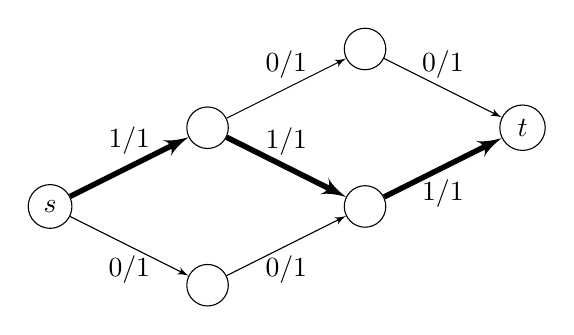
\begin{tikzpicture}
    \tikzset{vertex/.style = {shape=circle,draw,minimum size=1.5em}}
    \tikzset{edge/.style = {->,> = latex'}}

    \node[vertex] (a) at (0, 0) {$s$};
    \node[vertex] (b) at (2, -1) {};
    \node[vertex] (c) at (2, 1) {};
    \node[vertex] (d) at (4, 0) {};
    \node[vertex] (e) at (4, 2) {};
    \node[vertex] (f) at (6, 1) {$t$};

    \draw[edge] (a) -- (b) node [midway, below] {$0/1$};
    \draw[edge] (b) -- (d) node [midway, below] {$0/1$};
    \draw[edge] (c) -- (e) node [midway, above] {$0/1$};
    \draw[edge] (e) -- (f) node [midway, above] {$0/1$};

    \draw[edge, line width=2pt] (a) -- (c) node [midway, above] {$1/1$};
    \draw[edge, line width=2pt] (c) -- (d) node [midway, above] {$1/1$};
    \draw[edge, line width=2pt] (d) -- (f) node [midway, below] {$1/1$};

  \end{tikzpicture}
  \caption{A blocking flow is not a maximum flow.}
\end{figure}

\section{Dinic's Algorithm}
We can now formulate Dinic\footnote{Sometimes also transliterated as Dinitz.}'s algorithm: start with
$\ff = \veczero$, and then repeatedly add to $\ff$ a blocking flow $\hat{\ff}$ in $G_{\ff}$, until no more $s$-$t$ paths
exist in $G_{\ff}$.

Note that by doing a path decomposition on $\hat{\ff}$ and adding these paths to $\ff$ one by one, we see that
our algorithm is a `special case' of Ford-Fulkerson (with a particular augmenting path strategy) and hence
inherits all the behaviors/bounds we proved in the last chapter.

\begin{lemma}
  Let $\ff$ be a feasible flow, $\hat{\ff}$ a blocking flow in $G_{\ff}$ and define $\ff' = \ff+\hat{\ff}$ (think
  of $\ff$ and $\ff'$ to be the flows at some steps $k$ and $k+1$ in the algorithm). Then
  $\ell_{G_{\ff'}}(t) \geq \ell_{G_{\ff}}(t) + 1$.
\end{lemma}
\begin{proof}
  Let $L, L'$ be the edge sets of the level graphs of $G_{\ff}, G_{\ff'}$
  respectively.
  % \todo{I didn't really
  %   get the proof in the class for this part very well so I wrote my own. Feel
  %   free to change, I hope it's okay though.}
  We would now like to show that $d_{L'}(s, t) \geq 1 + d_L(s, t)$. Let's first assume that in fact
  $d_{L'}(s, t) < d_L(s, t)$. Now take a shortest $s$-$t$ path in the level graph of
  $G_{\ff'}$, say $s=v_0, v_1, \dots, v_{d_{L'}(s, t)} =  t$.
  Let $v_j$ be the first vertex along the path such that
  $d_{L'}(s, v_j) < d_L(s, v_j)$.
  As $d_{L'}(s, t) < d_L(s, t)$, such a $v_j$ must exist.

  We'd like to understand the edges in the level
  graph $L'$.
  Let $E(G_{\ff})$ denote the edges of the $G_{\ff}$,
  and let $\operatorname{rev}(L)$ denote the set of
  reversed edges of $L$.
  The level graph edges of $G_{\ff'}$ must satisfy
  $L' \subseteq L \union
  \operatorname{rev}(L) \union (E(G_{\ff}) \setminus
  L)$.

  In our $s$-$t$ path in $L'$, the vertex $v_j$ is reached by an edge from $v_{j-1}$,
  and the level of $v_{j-1}$ in $G_{\ff}$ is at most the level it receives in $G_{\ff'}$
  so the edge $(v_{j-1},v_j) \in L$ skips
  at least one level forward  in $G_{\ff}$.
  But, edges in $L$ do not skip a level in
  $G_{\ff}$, and edges in
  $\operatorname{rev}(L)$ or
  $E(G_{\ff}) \setminus L$ do not move from a lower level to higher
  level in $G_{\ff}$.
  So this edge cannot exist and we have reached a contradiction.
  % Write down the levels of the vertices in
  % $G_{\ff}$ along the path,
  % then
  % there are more levels in $G_{\ff}$ than
  % there are vertices in the path, so there must a be
  % level in $G$
  % so by the pigeonhole principle there must be a level in $G_{\ff}$ that
  % the path jumps over, i.e. there is some edge that jumps up more than one
  % level in $G_{\ff}$.
  % However, we claim this is impossible. Such an edge cannot exist in $G_{\ff}$ by definition of the level
  % graph. The only other edges in $G_{\ff'}$ are reversals of edges used in the blocking flow $\hat{\ff}$,
  % but by construction this flow only uses admissible edges in $G_{\ff}$ (i.e. edges that `step up' one
  % level). Hence the edge $(v_i, v_{i+1})$ cannot exist and we have arrived at a contradiction.

  Now suppose that $d_{L'}(s, t) = d_L(s, t)$. This means there is an $s$-$t$ path in $L'$ using
  edges in $L$ -- but such a path must contain an edge saturated by
  the blocking flow $\hat{\ff}$.

  (Note: the reason this path must use only edges in $L$ is similar to
  the previous case: the other possible types of edges do not move
  to higher levels in $G_{\ff}$ at all, making the path too long if we use any of them.)

  So we must have $d_{L'}(s, t) \geq 1 + d_L(s, t)$.
\end{proof}
An immediate corollary of this lemma is the convergence of Dinic's algorithm:
\begin{theorem}
  Dinic's algorithm terminates in $O(n)$ iterations.
\end{theorem}
\begin{proof}
  By the previous lemma, the level of $t$ increases by at least one each iteration. A shortest path
  can only contain each vertex once (otherwise it would contain a cycle) so the level of any vertex
  is never more than $n$.
\end{proof}

For graphs with unit capacities ($c = 1$) we can prove even better bounds on the number of iterations.
\begin{theorem}
  On unit capacity graphs, Dinic's algorithm terminates in
  $$O\left(\min\{m^{1/2}, n^{2/3}\}\right)$$ iterations.
\end{theorem}
\begin{proof}
  We prove the two bounds separately.
  \begin{enumerate}
  \item Suppose we run Dinic's algorithm for $k$ iterations, obtaining a flow $\ff$ that is
    feasible but not necessarily yet optimal. Let $\tilde{\ff}$ be an optimal flow in
    $G_{\ff}$ (i.e. $\ff+\tilde{\ff}$ is a maximum flow for the whole graph),
    and consider a path decomposition of $\tilde{\ff}$. Since after $k$ iterations
    any $s$-$t$ path has length $k$ or more, we use up a total capacity of at least
    $\text{val}(\tilde{\ff})k$ across all edges. But the edges in $G_{\ff}$ are either edges
    from the original graph $G$ or their reversals (but never both) meaning the total
    capacity of $G_{\ff}$ is at most $m$, hence $\text{val}(\tilde{\ff}) \leq m/k$.

    Recalling our earlier observation that our algorithm is a special case of
    Ford-Fulkerson, this implies that our algorithm will terminate after at most
    another $m/k$ iterations. Hence the number of iterations is bounded by $k+m/k$ for
    any $k>0$. Substituting $k=\sqrt{m}$ gives the first desired bound.
  \item Suppose again that we run Dinic's algorithm for $k$ iterations obtaining a flow $\ff$.
    The level graph of $G_{\ff}$ partitions the vertices into sets
    $D_i = \{u\mid\ell(u) = i\}$ for $i\geq 0$.
    As shown before, the sink $t$ must be at a level of at
    least $k$, meaning we have at least this many non-empty levels starting from
    $D_0 = \{s\}$. To simplify, discard all vertices and levels beyond $D_{\ell(t)}$.

    Now, consider choosing a level $I$ uniformly at random from
    $\setof{1,\ldots,k}$.
    Since there are at most $n-1$ vertices in total across these levels,
    $\E{\abs{D_I}} \leq (n-1)/k$, and by Markov's inequality
    \[
      \Pr[ \abs{D_I} \geq 2n/k ] \leq
      \frac{(n-1)/k}{2n/k} < \frac{1}{2}
      .
    \]
    % \todo{I found this a bit easier to follow than Markov, feel free to change (again).}
    % divide the levels into two groups: those with $|D_i|\leq 2n/k$ and those with
    % $|D_i| > 2n/k$. If the latter group contained at least $k/2$ levels then together
    % they would contain strictly more than $(2n/k)\cdot(k/2) = n$ vertices, which is a
    % contradiction (note the $D_i$ are disjoint), so more than $k-k/2 = k/2$ levels
    % satisfy the first condition,

    Thus strictly more than $k/2$ of the levels $i \in \setof{1,\ldots,k}$
    have $\abs{D_i} < 2n/k$ and so there must be two adjacent levels $j$, $j+1$
    for which this upper bound on the size holds.
    There can be at most
    $|D_j|\cdot|D_{j+1}| \leq 4n^2/k^2$ edges between these levels, and by the min-cut
    max-flow theorem we saw in the previous chapter, this is an upper bound on the flow
    in $G_{\ff}$, and hence on the number of iterations still needed for our algorithm to
    terminate.

    This means the number of iterations is bounded by $k + 4n^2/k^2$ for any $k>0$,
    which is $O(n^{2/3})$ at $k=2n^{2/3}$.
  \end{enumerate}
\end{proof}

\section{Finding Blocking Flows}
 \label{sec:findBlockingFlows} 
What has been missing from our discussion so far is the process of actually finding a blocking flow.
We can achieve this using repeated depth-first search. We repeatedly do a search in the level graph (so
only using edges $L$) for $s$-$t$ paths and augment these. We erase edges whose subtrees have been
exhausted and do not contain any augmenting paths to $t$. Pseudocode for the algorithm is given below.

\begin{algorithm}[H]
  \SetAlgoLined
  $\ff \leftarrow \veczero$\;
  $H \leftarrow L$\;
  \Repeat{
    $P\leftarrow\text{\textsc{Dfs}}(s, H, t)$\;
    \eIf{$P\neq\emptyset$}{
      Let $\hat{\ff}$ be a flow that saturates path $P$.\\
      $\ff\leftarrow \ff+\hat{\ff}$\;
      Remove from $H$ all edges saturated by $\hat{\ff}$.
    }{
      \Return{\ff}\;
    }
  }
  \caption{\textsc{FindBlockingFlow}}
\end{algorithm}

\begin{algorithm}[H]
  \SetAlgoLined
  \If{$u=t$}{\Return{\textnormal{the path $P$ on the dfs-stack.}}}
  \For{$(u,v)\in H$}{
    $P\leftarrow\text{\textsc{Dfs}}(v, H, t)$\;
    \eIf{$P\neq\emptyset$}{
      \Return{$P$}\;
    }{
      Erase $(u, v)$ from $H$.
    }
  }
  \Return{$\emptyset$}\;
  \caption{\textsc{Dfs}(u, H, t)}
\end{algorithm}

\begin{lemma}
  For general graphs, \textsc{FindBlockingFlow} returns a blocking flow in $O(nm)$ time.
  Hence Dinic's algorithm runs in $O(n^2 m)$ time on general capacity graphs.
\end{lemma}
\begin{proof}
  % We sketch an approach to amortized analysis of the running time.
  First, consider the amount of work spent pushing edges onto the
  stack which eventually results in augmentation along an $s$-$t$ path
  consisting of those edges (i.e.\ adding flow along that path).
  Since each augmenting path saturates at least one edge,  we do at most $m$ augmentations. Each
  path has length at most $n$.
  Thus the total amount of work pushing these edges to the stack, and removing them
  from the stack upon augmentation, and deleting saturated edges, can
  be bounded by $O(mn)$.
  Now consider the work spent pushing edges onto the stack which are
  later deleted because we ``retreat'' after not finding an $s$-$t$.
  An edge can only be pushed onto the stack once in this way, since it
  is then deleted. So the total amount spent pushing edges to the
  stack and deleting them this way is $O(m)$.
   % First, consider the amount of work spent pushing edges onto the
  % Since each augmenting path saturates at least one edge, there are at most $m$ augmenting paths. Each
  % path has length at most $n$.
  % Hence the calls to \textsc{Dfs} that result in augmenting paths account for
  % $O(mn)$ work jointly. The calls to \textsc{Dfs} that do not result in an augmenting path together account
  % for $O(m)$ work because each such call erases an edge, meaning across the whole algorithm run there are at
  % most $m$ such calls.
\end{proof}
\begin{lemma}
  For unit capacity graphs, \textsc{FindBlockingFlow} returns a blocking flow in $O(m)$ time. Hence Dinic's
  algorithm runs in $O\left(\min\{m^{3/2}, mn^{2/3}\}\right)$ time on unit capacity graphs.
\end{lemma}
\begin{proof}
  When our depth-first search traverses some edge $(u, v)$, one of two things will happen: either we find no
  augmenting path in the subtree of $v$, leading to the erasure of this edge, or we find an augmenting path
  which will necessarily saturate $(u, v)$, again leading to its erasure. This means each edge will be
  traversed at most once by the depth-first search.
\end{proof}

Another interesting bound on the runtime, which we will not prove here, is that Dinic's algorithm will run in
$O\left(\abs{E}\sqrt{\abs{V}}\right)$ time on bipartite matching graphs.

\section{Minimum Cut as a Linear Program}
Finally we show that minimum cut may be formulated as a linear program. For a subset $S \subseteq V$ write
$c_G(S)$ for the sum of $\cc(e)$ over all edges $e = (u, v)$ that cross the cut, i.e.\ $u \in S, v\not\in S$.
Note that `reverse' edges are not counted in this cut. The minimum cut problem asks us to find some $S\subseteq V$
such that $s\in S$ and $t\not\in S$ such that $c_G(S)$ is minimal.
\begin{align}
  \begin{aligned}
    \min_{S\subseteq V} \quad &c_G(S) \\
    s.t.\quad & s \in S \\
    &t\not\in S\\
  \end{aligned}
  \label{prog0}
\end{align}

We claim this is equivalent to the following
minimization problem:
\begin{align}
  \begin{aligned}
    \min_{\xx \in \R^{V}} \quad &\sum_{e\in E} \cc(e) \max\left\{\bb_e^\trp \xx, 0\right\} \\
    s.t. \quad & \xx(s) = 0 \\
    & \xx(t) = 1 \\
    &\veczero\leq \xx\leq \vecone \\
  \end{aligned}
  \label{prog1}
\end{align}
Recall $\bb_e^\trp \xx = \xx(v) - \xx(u)$ for $e = (u, v)$.
We can rewrite this as a proper linear program by
introducing extra variables for the maximum:
\begin{align}
  \begin{aligned}
    \min_{\xx \in \R^{V}, \uu \in \R^{E}} \quad & \cc^\trp \uu \\
    s.t. \quad & \bb_{s,t}^\trp\xx = 1 \\
    &\veczero\leq \xx\leq \vecone \\
    &\uu \geq \veczero \\
    &\uu \geq \BB^\trp \xx \\
  \end{aligned}
  \label{prog2}
\end{align}
And, in fact, we'll also see that we don't need the constraint
$\veczero\leq \xx\leq \vecone$, leading to the following simpler
program:
\begin{align}
  \begin{aligned}
    \min_{\xx \in \R^{V}, \uu \in \R^{E}} \quad & \cc^\trp \uu \\
    s.t. \quad & \bb_{s,t}^\trp\xx = 1 \\
    &\uu \geq \veczero \\
    &\uu \geq \BB^\trp \xx \\
  \end{aligned}
  \label{prog3}
\end{align}

This last linear program is the dual program to the maximum flow linear program.

\begin{lemma}
  Programs \eqref{prog0}, \eqref{prog2}, and \eqref{prog3} have equal optimal values.
\end{lemma}
\begin{proof}
  We start by considering equality between optimal values of Program
  \eqref{prog0} and Program \eqref{prog2}
  Let $S$ be an optimal solution to Program~\eqref{prog0} and take $\xx = \vecone_{V\setminus S}$. Then $\xx$ is a
  feasible solution to Program~\eqref{prog2} with cost equal to $c_G(S)$.

  Conversely, suppose $\xx$ is an optimal solution to Program~\eqref{prog2}. Let $\alpha$ be uniform in $[0,1]$ and define
  $S = \{v\in V\mid\xx(v) \leq \alpha\}$. This is called a threshold cut.
  We can verify that
  \[ \Pr\left[\text{$e$ is cut by $S$}\right] = \max\{\bb_e^\trp \xx, 0\}. \]
  and hence $\mathbb{E}_t [c_G(S)]$ is exactly the optimization function of \ref{prog1} (and hence
  \ref{prog2}).
  Since at least one outcome must do as well as the average, there is a subset $S\subseteq V$ achieving this value
  (or less).

  We can use the same threshold cut to show that we can round a
  solution to Program~\eqref{prog3} to an equal or smaller value cut
  feasible for Program~\eqref{prog0}. The only difference is that in
  this case, we get
  \[
    \Pr\left[\text{$e$ is cut by $S$}\right] \leq \max\{\bb_e^\trp \xx, 0\}
  \]
  which is still sufficient.
\end{proof}


%%% Local Variables:
%%% mode: latex
%%% TeX-master: "agao21_script"
%%% End:

%\end{document}

\chapter{Link-Cut Trees}
\newcommand{\key}{\operatorname{key}}
\newcommand{\prio}{\operatorname{prio}}

In this chapter, we will learn about a dynamic data structure that allows us to speed-up Dinic's algorithm even more: \emph{Link-Cut Trees}. This chapter is inspired by lecture notes of Richard Peng\footnote{CS7510 Graph Algorithms Fall 2019, Lecture 17 at \url{https://faculty.cc.gatech.edu/~rpeng/CS7510\_F19/}} and the presentation in a very nice book on data structures and network flows by Robert Tarjan \cite{tarjan1983data}.

\section{Overview}

\paragraph{Model.} We consider a directed graph $G=(V,E)$ that is undergoing \emph{updates} in the form of edge insertions and/or deletions. We number the graph in its different \emph{versions} $G^0, G^1, G^2, \dots$ such that $G^0$ is the initial input graph, and $G^i$ is the initial graph after the first $i$ updates were applied. Such a graph is called a \emph{dynamic} graph.

In this lecture, we restrict ourselves to \emph{dynamic rooted forests} that is we assume that every $G^i$ forms a directed forest where in each forest a single root vertex is reached by every other vertex in the tree. For simplicity, we assume that $G^0 = (V, \emptyset)$ is an empty graph.

\begin{figure}[!ht]
    \centering
    \includegraphics[scale=0.2]{./fig/InsertionDynamicTree_lectureDynamicTree.jpeg}
    \caption{The $i^{th}$ version of $G$ is a rooted forest. Here, red vertices are roots and there are two trees. The $(i+1)^{th}$ version of $G$ differs from $G^i$ by a single edge that was inserted (the blue edge). Note that edge insertions are only valid if the tail of the edge was a root. In the right picture, the former root on the right side is turned into a normal node in the tree by the update.}
    %\label{fig:my_label}
\end{figure}

\paragraph{The Interface.} Let us now describe the interface of our data structure that we call a link-cut tree. We want to support the following operations:
\begin{itemize}
    \item $\textsc{Initialize}(G)$: Creates the data structure initially and returns a pointer to it. Each vertex is initialized to have an associated cost $cost(v)$ equal to $0$.
    \item $\textsc{FindRoot}(v)$: Returns the root of vertex $v$. 
    \item $\textsc{AddCost}(v, \Delta)$: Add $\Delta$ to the cost of every vertex on the path from $v$ to the root vertex $\textsc{FindRoot}(v)$.
    \item $\textsc{FindMin}(v)$: Returns tuple $(w, cost(w))$ where $w$ is the (first) vertex on the path from $v$ to $\textsc{FindRoot}(v)$ of lowest cost. 
    \item $\textsc{Link}(u,v)$: Links two trees that contain $u$ and $v$ into a single tree by inserting the edge $(u,v)$. This assumes that $u, v$ are initially in different trees and $u$ was a root vertex.
    \item $\textsc{Cut}(u,v)$: Cuts the edge $(u,v)$ from the graph which causes the subtree rooted at $u$ to become a tree and $u$ to become a root vertex. Assumes $(u,v)$ is in the current graph.
\end{itemize}

\paragraph{Main Result.} The following theorem is the main result of today's lecture.

\begin{theorem}\label{thm:mainTheoremLinkCutTree}
We can implement a link-cut tree such that any sequence of $m$ operations takes total expected time $O(m \log^2 n + |V|)$.
\end{theorem}



\section{Balanced Binary Search Trees: A Recap}
In \href{https://kyng.inf.ethz.ch/courses/APC21/Chapter_2.pdf}{Chapter 2 of the course Algorithms, Probability and Computing}, we introduced (balanced) binary search trees, and studied \emph{treaps}, which are a simple randomized approach to building a binary search tree with good performance, at least in expectation.
If you are not familiar with balanced binary search trees, we encourage you to read this chapter from the APC script. 
That said, we will quickly recap the important properties of binary search trees and treaps.
If you're already familiar with treaps, you can skip ahead to the next section to see how we use them for building Link-Cut trees.
%

\paragraph{Binary Search Trees.} A binary search tree $\mathcal{T}$ is a data structure for keeping track of a set of \emph{items} where each item has a \emph{key} associated with it.
The data structure stores the items in a rooted binary tree with a node for each item, and maintains the property for each node $v$, all items in the \emph{left} subtree of $v$ have keys less than $v$, and all items in the \emph{right} subtree of $v$ have keys greater than $v$.
This is called the \emph{search property} of the tree, because it makes it simple to search through the tree to determine if it contains an item with a given key.

The binary search trees we studied in APC supported the following operations, while maintaining the search property:
\begin{description}
\item[insert:] We can add an item to the tree with a specified key.
\item[delete:] We can remove an item from the tree with a specified key.
\item[find:] Determine if the tree contains an item with a specified key.
\item[split:] Suppose the tree contains two items $v_1$ and $v_2$ with keys $k_1$ and $k_2$ where $k_1 < k_2$, and suppose no item in tree has a key $k$ in the interval $(k_1,k_2)$. Then the split operation applied to these two items should split the current tree into two: One tree containing all items with keys in $(-\infty,k_1]$ and the other with all items in $[k_2,\infty)$.
\item[join:] Given two binary search trees, one with keys in the interval $(-\infty,k]$, the other with keys in the interval $(k,\infty)$, form a single binary search tree containing the items of both.
\end{description}

\paragraph{Search-Property-Preserving Tree rotations.} In this chapter, we will use that enforcing the search property in a binary tree still leaves various options to have a tree. In fact, there is a classic tree operation that preserves the search property while changing the tree: Tree rotations. 

A tree rotation makes a local change to the tree by changing only a constant number of pointers around, while preserving the search property.
Given two items $v_1$ and $v_2$ such that $v_1$ is a child of $v_2$, a tree rotation applied to these two nodes will make $v_2$ the child of $v_1$, while moving their subtrees around to preserve the search property. This is shown in Figure~\ref{fig:binaryTreeRotation}.
When the rotation makes $v_2$ the right child of $v_1$ (because $v_2$ has the larger key), this is called a \emph{right rotation}, and when it makes $v_2$ the left child of $v_1$ (because $v_2$ has a smaller key), it is called a \emph{left rotation}.

\begin{figure}[ht]
    \centering
    \includegraphics[width=0.8\textwidth]{./fig/TreeRotation_lectureDynamicTree.png}
    \caption{Given two items $v_1$ and $v_2$ such that $v_1$ is a child of $v_2$, a tree rotation applied to these two nodes will make $v_2$ the child of $v_1$, while moving their subtrees around to preserve the search property. This figure shows a \emph{right rotation}.}
    \label{fig:binaryTreeRotation}
  \end{figure}

\paragraph{Balanced BSTs.} To implement the operations given above efficiently,  one needs to ensure that the BST always stays of bounded depth (normally $O(\log n)$). This is typically ensured by making tree rotations. In the rest of the chapter, we use a randomized strategy that ensures that the depth of the tree is $O(\log n)$ in expectation. The obtained data structure is often referred to as \emph{treap}.  We will not give the details here, but instead explicitly construct one in the next section and give a full (although brief) analysis.

\section{A Data Structure for Path Graphs}

Before we prove \Cref{thm:mainTheoremLinkCutTree} in its full generality, let us reason about implementing a link-cut tree data structure in a weaker setting: we assume that every version $G^i$ of $G$ is just a collection of rooted vertex-disjoint paths.
We will later build on the routines we develop for the path case to construct the data structure for the general tree case.
To distinguish the routines we develop for paths from those we develop for the general case, we will prefix the path-case routines with a ``P'', i.e. we denote our implementations of $\textsc{FindRoot}, \textsc{AddCost}, \textsc{FindMin}, \textsc{Link},$ and $\textsc{Cut}$ by $\textsc{PFindRoot}, \textsc{PAddCost}, \textsc{PFindMin}, \textsc{PLink},$ and $\textsc{PCut}$.

\paragraph{Representing Paths via Balanced Binary Search Trees.} It turns out that paths can be represented rather straight-forwardly via Balanced Binary Search Trees, with an node/item for each vertex of the graph. For the sake of concreteness, we here use \emph{treaps} to represent paths\footnote{If you have not seen treaps before, don't worry, they are simple enough to understand them from our application here. }.
Most other balanced binary search trees would also work.

Note that we now represent each rooted path with a tree, and this tree has its own root, which is usually \emph{not} the root of the path. To minimize confusion, we will refer to the root of the path as the \emph{path-root} and the root of the associated tree as the \emph{tree-root} (or \emph{subtree-root} for the root of a subtree).

In our earlier discussion of binary trees, we always assumed each item has a key: Instead we will now let the key of each vertex correspond to its distance to the path-root in the path that contains it.
We will make sure the treap respects the search property w.r.t. this set of keys/ordering, but we will not actually explicitly compute these keys or store them.
Note one important difference to the scenario of treaps-with-keys: When we have two paths, with path-roots $r_1$ and $r_2$, we will allow ourselves to join these paths in two different ways: either so that $r_1$ or $r_2$ becomes the overall path-root.

Let us describe how to represent a path $P$ in $G$. First, we pick for each vertex $v$, we assign it a \emph{priority} denoted $\prio(v)$, which we choose to be a uniformly random integer sampled from a large universe, say $[1, n^{100})$. We assume henceforth that $\prio(v) \neq \prio(w)$ for all $v \neq w \in V$.

Then, for each path $P$ in $G$, we store the vertices of $P$ in a binary tree, in particular a treap, $\mathcal{T}_{P}$ and enforce the following invariants:
\begin{itemize}
      \item \textbf{Search-Property}: for all $v$, $left_{\mathcal{T}_{P}}(v)$ precedes $v$ on $P$ and $right_{\mathcal{T}_{P}}(v)$ appears later on $P$ than $v$. See the Figure~\ref{fig:PathAsTreap} below for an illustration.
    \item \textbf{Heap-Order}: for each vertex $v \in P$, its parent $w = parent_{\mathcal{T}_{P}}(v)$ in $\mathcal{T}_{P}$ is either $NULL$ (if $v$ is the path-root) or has $\prio(v) > \prio(w)$.
\end{itemize}

\begin{figure}[!ht]
    \centering
    \includegraphics[width=0.8\textwidth]{./fig/PathRepTreap_lectureDynamicTree.png}
    \caption{In the upper half of the picture, the original path $P$ in $G$ is shown, along with the random numbers $\prio(v)$ for each $v$. The lower half depicts the resulting treap with vertices on the same vertical line as before.}
    \label{fig:PathAsTreap}
\end{figure}

\paragraph{Depth of Vertex in a Treap.} Let us next analyze the expected depth of a vertex $v$ in a treap $\mathcal{T}_{P}$ representing a path $P$. Let $P = \langle x_1, x_2, \dots, x_k = v, \dots, x_{|P|}\rangle$, i.e. $v$ is the $k^{th}$ vertex on the path $P$. Observe that a vertex $x_i$ with $i < k$ is an ancestor of $v$ in $\mathcal{T}_{P}$ if and only if no vertex $\{x_{i+1}, x_{i+2}, \dots, x_k\}$ has received a smaller random number than $\prio(x_i)$. Since we sample $\prio(w)$ uniformly at random for each $w$, we have that $\mathbb{P}[x_i \text{ ancestor of } v] = \frac{1}{k-i+1}$. The case where $i > k$ is analogous and has $\mathbb{P}[x_i \text{ ancestor of } v] = \frac{1}{i-k+1}$. Letting $X_i$ be the indicator variable for the event that $x_i$ is an ancestor of $v$, it is straight-forward to calculate the expected depth of $v$ in $\mathcal{T}_{P}$:
\[
    \mathbb{E}[depth(v)] = \sum_{i \neq k} \mathbb{E}[X_i] =  \sum_{i = 1}^{k-1}\frac{1}{k-i+1} + \sum_{i = k+1}^{|P|} \frac{1}{i-k+1} = H_k + H_{|P|-k+1} - 2 = O(\log |P|)
\]
It is straight-forward to see that the operation $\textsc{PFindRoot}(v)$ can thus be implemented to run in expected $O(\log n)$ time by just iteratively following the parent pointers starting in $v$.

\paragraph{Implementing $\textsc{PFindRoot}(v)$.} From any vertex $v$, we can simply follow the parent pointers in $\mathcal{T}_{P}$ until we are at the tree-root of $\mathcal{T}_{P}$. Then, we find the right-most child of $\mathcal{T}_{P}$ by following the $right_{\mathcal{T}_{P}}$ pointers. Finally, we return the right-most child which is the path-root. Since the paths from $v$ is at depth $O(\log n)$ in expectation, and so is the path-root of $v$, we have that this operation can be executed in $O(\log n)$ expected time.

\paragraph{Extra fields to help with $\textsc{PAddCost}(v, \Delta)$ and $\textsc{PFindMin}(v)$.} The key trick to do the Link-Cut tree operations efficiently is to store the change to subtrees instead of updating $cost(v)$ for each affected vertex. 

To this end, we store two fields $\Delta cost(v)$ and $\Delta min(v)$ for every vertex $v$. We let $cost(v)$ be the cost of each vertex, and $mincost(v)$ denote the minimum cost of any descendant of $v$ in $\mathcal{T}_{P}$ (where we let $v$ be a descendant of itself). 
A warning: the $mincost(v)$ value is the minimum cost in the treap-subtree; \emph{not} the minimum cost on the path between $v$ and the path-root that could be different.
Note also that we do not explicitly maintain these fields.

Then, we maintain for each $v$
\[
    \Delta cost(v) = cost(v) - mincost(v)
\]
\[
    \Delta min(v) = \begin{cases}
    mincost(v) & parent_{\mathcal{T}_{P}}(v) = NULL, \\
    mincost(v) - mincost(parent_{\mathcal{T}_{P}}(v)) & otherwise\end{cases}
\]
With a bit of work, we can see that with these definitions, we obtain $mincost(v) = \sum_{w \in \mathcal{T}_{P}[v]} \Delta min(w)$ where $\mathcal{T}_{P}[v]$ is the $v$-to-tree-root path in $\mathcal{T}_{P}$. We can then recover $cost(v) = mincost(v) + \Delta cost(v)$. We say that henceforth, that an operation/manipulation to the tree is \emph{field-preserving} if the fields  $\Delta min(v)$ and $\Delta cost(v)$ satisfy the equations above.

\paragraph{Implementing $\textsc{PAddCost}(v, \Delta)$ and $\textsc{PFindMin}(v)$ -- the easy way.}
First, we will discuss ways to implement $\textsc{PAddCost}$ and $\textsc{PFindMin}$ in ways that rely on the fact that $\textsc{PLink}$ and $\textsc{PCut}$ are field-preserving.

$\textsc{PAddCost}(v, \Delta)$ is very easy: First, consider the case when $v$ has no predecessor on the path. If this is the case, we can simply find the tree-root of the tree $\mathcal{T}_{P}$ containing $v$ and at this root increase the value of the field $mincost$ by $\Delta$. This implicitly increases the cost of all nodes in the tree by $\Delta$.
Second, consider the case when $v$ has a predecessor $u$ in the path (we can store these explicitly, or we can search for it in the tree). Call $\textsc{PCut}(u,v)$ -- now $v$ no longer has a predecessor and we can proceed as before. Finally, call $\textsc{PLink}(u,v)$. That's it.

Implemeting  $\textsc{PFindMin}(v)$ is also very easy: First, consider the case when $v$ has no predecessor on the path.  Again, we can find the tree-root $r$ of the tree $\mathcal{T}_{P}$ containing $v$.
By definition $mincost(r)$ is the minimum cost across the whole tree, and hence across the path between $v$ and the path-root. We can also find the node with the minimum cost: Search in the tree, starting from the tree-root, and, if possible follow the child where $\Delta min(v)=0$ (going left if both are eligible). Eventually, we get to a node where there is no child with $\Delta min(v) = 0$. This must be a minimizer.
Now, to deal with the case where $v$ has a predecessor, we do the same we did for $\textsc{PAddCost}$: Find the predecessor $u$, call  $\textsc{PCut}(u,v)$, then find the minimizer, finally call  $\textsc{PLink}(u,v)$.

\paragraph{Implementing $\textsc{PAddCost}(v, \Delta)$ and $\textsc{PFindMin}(v)$ -- the hard way.}
We can also implement $\textsc{PAddCost}(v, \Delta)$ and $\textsc{PFindMin}(v)$ without relying on $\textsc{PLink}$ and $\textsc{PCut}$, which is more efficient, but also more unpleasant\footnote{You don't have to know these more complicated approaches for the exam, but we include them for the interested reader.}.

To implement the operation $\textsc{PFindMin}(v)$ more efficiently, consider the sequence of nodes on the path in the tree $\mathcal{T}_{P}$ (not the path $P$) between $v$ and the path-root. First let $v = x_1, x_2, \ldots, x_k = r$ be the nodes leading to the tree-root if $v$ is left of the tree root, and then let $y_1, \ldots, y_l$ be the remaining nodes on the tree path to the path-root.
Observe that either the minimizer one of these nodes (which we can check by checking their $\Delta min$), or it is in a right subtree of some $x_i$, or in any subtree of some $y_j$. So we just search through these subtrees for their minimizers (looking for  $\Delta min(v)=0$ ) and pick the best one. There will only be $O(\log n)$ trees in expectation.

Next, let us discuss the implementation of the operation $\textsc{PAddCost}(v, \Delta)$ which is given in pseudo-code above. The first for-loop of this algorithm ensures that the tree is again \emph{field-preserving}. This is ensured by walking down the path from the path-root of $v$ to $v$ and whenever we walk to the left, we make sure to increase all costs in the right subtree by adding $\Delta$ to the subtree-root of the right subtree $r$ in the form of adding it to $\Delta min(r)$. On the vertices along the path it updates the costs by using the $\Delta cost(\cdot)$ fields. It is easy to prove from this that thereafter the tree is  \emph{field-preserving}.

\begin{algorithm}
  \SetAlgoLined
  \DontPrintSemicolon
  \SetKwRepeat{Do}{do}{while}
  Store the vertices on the path in the tree $\mathcal{T}_{P}$ between $v$ and the path-root, i.e. $\langle v = x_1, x_2, \ldots, x_k = \textsc{PFindRoot}(v)\rangle$.\\
  \For{$i = k$ down to $1$}{
        $\Delta cost(x_i) = \Delta cost(x_i) + \Delta$.\;
        \If{$(r \gets right_{\mathcal{T}_{P}}(x_i)) \neq NULL$ AND ($i = 0$ OR $x_{i-1} \neq r$)}{
            $\Delta min(r) \gets \Delta min(r) + \Delta$
        }
  }
  
  \For{$i = 1$ up to $k$}{
        $\textit{minval}  \gets \Delta cost(x_i)$.\\
        \lForEach{$w \in \{left_{\mathcal{T}_{P}}(x_i), right_{\mathcal{T}_{P}}(x_i)\}, w \neq NULL$}{
            $\textit{minval} \gets \min\{ \textit{minval} , \Delta min(w)\}$.
        }
        
        $\Delta min(x_i) \gets \Delta min(x_i) + \textit{minval}$.\\
        $\Delta cost(x_i) \gets \Delta cost(x_i) - \textit{minval}$.\\
        \lForEach{$w \in \{left_{\mathcal{T}_{P}}(x_i), right_{\mathcal{T}_{P}}(x_i) \}, w \neq NULL$}{
            $\Delta min(w) \gets \Delta min(w) - \textit{minval} $.
        }
  }
  \caption{$\textsc{PAddCost}(v, \Delta)$}
\end{algorithm}

While after the first for-loop the values can be computed efficiently, we might now be in the situation that $\Delta min(w)$ or/and $\Delta cost(w)$ are negative for some vertices $w$. We may also  violate the invariants we want to preserve on the relationship between the $\Delta min(w)$ or/and $\Delta cost(w)$ fields and the true $cost$ and $mincost$ values at each node. We recover through the second for-loop that at each vertex on the tree path from $v$ to its path-root first computes the correct minimum in the subtree again (using the helper variable $\textit{minval}$) and then adjusts all values in its left/right subtree and its own fields. Since we argued that $v$ is at expected depth $O(\log(n))$, we can see that this can be done in expected $O(\log n)$ time.


\paragraph{Implementing $\textsc{PCut}(u,v)$.} Let us first assume that we have a dummy node $d_0$ with $\prio(d_0) = 0$ in the vertex set. The trick is to first treat the operation as splitting the edge $(u,v)$ into $(u,d_0)$ and $(d_0,v)$ by inserting the vertex $d_0$ in between $u$ and $v$ in the tree $\mathcal{T}_{P}$ as a leaf (this is always possible). Then, we can do standard binary tree rotations to re-establish the heap-order invariant (see \Cref{fig:PCutRotation}). It is not hard to see that after $O(\log n)$ tree rotations in expectation, the heap-order is re-established and $d_0$ is at new tree-root of $\mathcal{T}_{P}$. It remains to remove $d_0$ and make $left_{\mathcal{T}_{P}}(d_0)$ and $right_{\mathcal{T}_{P}}(d_0)$ tree-roots.

\begin{figure}[!ht]
    \centering
    \includegraphics[scale=0.2]{./fig/PathCutOperation_lectureDynamicTree.jpeg}
    \caption{For $\textsc{PCut}(u,v)$, we insert a vertex $d_0$ as a leaf of either $u$ or $v$ to formally split $(u,v)$ into $(u,d_0)$ and $(d_0,v)$ (this is shown on the left). While this preserves that Search-Property, it will violate the Heap-Order. Thus, we need to use tree rotations (shown on the left) to push $d_0$ to the top of the tree $\mathcal{T}_{P}$ (the arrow between the tree rotations should point in both ways).}
    \label{fig:PCutRotation}
\end{figure}

In the exercises for this week, we ask you to come up with the pseudo-code for \emph{field-preserving} tree rotations that still executes each rotation in $O(1)$ time.  Given this routine, we can then show that the implementation of  $\textsc{PCut}(u,v)$ is field-preserving overall. And since the number of rotations is bound by $O(\max\{depth(u), depth(v)\})$ and thus the time to execute the entire procedure is $O(\log n)$ in expectation.

%To ensure that the fields are correctly adjusted, we can make the $\Delta min(\cdot)$ values of the two vertices that are rotated equal to zero while ensuring that the tree is still \emph{field-preserving} by changing the $\Delta min(\cdot)$ fields of the (at most 3) subtree-roots of the subtrees to be rotated, and adapting the $\Delta cost(\cdot)$ fields of the two vertices to be rotated. Then, after the rotation, it is not hard to see that the tree is still \emph{field-preserving} and that the procedure applied in the second for-loop of the operation $\textsc{PAddCost}(v, \Delta)$ can then just be applied to the two rotated vertices and the subtree-roots of their subtrees. This ensures that the fields are maintained correctly. All of these operations can be implemented in $O(1)$ time per tree rotation.
%Note that  $\textsc{PCut}$ is basically just the treap split operation.


\paragraph{Implementing $\textsc{PLink}(u,v)$.} Implementing $\textsc{PLink}(u,v)$ could be done by reversing the process described above: we use a dummy vertex $d_0$ with priority $0$, and add it as the right child of $u$. We use tree rotations to then obtain heap-order again. Now,  we can make $v$ the right child of $d_0$. Note that the resulting tree has the search and the heap-order properties. 

It remains to get rid of $d_0$. To achieve this, we change its priority to $\infty$ (or say $n^{100}$), and then use tree rotations to obtain heap-order again. Since $d_0$ is the only vertex that violates the heap-order, this step results in $d_0$ being rotated downwards until it is a leaf. Then we can remove $d_0$ entirely. 

Again, it is not hard to see that the implementation runs in $O(\log n)$ expected time.

\paragraph{Notes.} The operations $\textsc{PLink}/ \textsc{PCut}$ can be implemented using almost all Balanced Binary Search Trees (especially the ones you have seen in your first courses on data structures). Thus, it is not hard to get a $O(\log n)$ worst-case time bound for all operations discussed above.

\section{Implementing Trees via Paths}

We now use the result from last section as a black box to obtain \Cref{thm:mainTheoremLinkCutTree}.

\paragraph{Path Decomposition.} For each rooted tree $T$, the idea is to decompose $T$ into paths. In particular, we decompose each $T$ into a collection of vertex-disjoint paths $P_1, P_2, \dots, P_k$ such that each internal vertex $v$ in $T$ has exactly one incoming edge in some $P_i$. We call the edges on some $P_i$  \emph{solid} edges and say that the other edges are \emph{dashed}. 

We maintain the paths $P_1, P_2, \dots, P_k$ using the data structure described in the last section. To avoid confusion, we use the prefix $P$ when we invoke operations of the path data structure, for example $\textsc{PFindRoot}(v)$ finds the root of $v$ in the path graph $P_i$ where $v \in P_i$.
We no longer need to think about the balanced binary trees that are used internally to represent each $P_i$. Instead, in this section, we use path-root to refer to the root of a path $P_i$ and we use tree root (or just root) to refer to a root of one of the trees in our given collection of rooted trees.

\begin{figure}[!ht]
    \centering
    \includegraphics[scale=0.20]{./fig/HeavyLightDecomposition_lectureDynamicTree.jpeg}
    \caption{The dashed edges are the edges not on any path $P_i$. The collection of (non-empty) paths $P_1, P_2, \dots, P_k$ can be seen to be the maximal path segments of solid edges.}
\end{figure}

\paragraph{The $\textsc{Expose}(v)$ Operation.} We start by discussing the most important operation of the data structure that will be used by all other operations internally: the operation $\textsc{Expose}(v)$. This operation flips solid/dashed edges such that after the procedure the path from $v$ to its tree root in $G$ is solid (possibly as a subpath in the path collection). Below you can find an implementation of the procedure $\textsc{Expose}(v)$. 

\begin{algorithm}
  \SetAlgoLined
  $w \gets v$.\\
  \While{$(w' = parent_G(\textsc{PFindRoot}(w))) \neq NULL$}{
    Invoke $\textsc{PCut}(z,w')$ for the solid edge $(z,w')$ incoming to $w'$.\\
    $\textsc{PLink}(\textsc{PFindRoot}(w),w')$.\\
    $w \gets w'$.\\
  }
  \caption{\textsc{Expose}(v)}
\end{algorithm}

\paragraph{Implementing Operations via $\textsc{Expose}(v)$.} We can now implement link-cut tree operations by invoking $\textsc{Expose}(v)$ and then forwarding the operation to the path data structure. 
\begin{algorithm}[H]
  \SetAlgoLined
  $\textsc{Expose}(v)$; $\textsc{PAddCost}(v, \Delta)$
  \caption{$\textsc{AddCost}(v, \Delta)$}
\end{algorithm}
\begin{algorithm}[H]
  \SetAlgoLined
  $\textsc{Expose}(v)$; \Return $\textsc{PFindMin}(v)$
  \caption{\textsc{FindMin}(v)}
\end{algorithm}
\begin{algorithm}[H]
  \SetAlgoLined
  $parent_G(u) \gets v$\;
  \lIf{$v$ has an incoming solid edge $(z,v)$}{
    $\textsc{PCut}(z,v)$
  }
  $\textsc{PLink}(u,v)$
  \caption{\textsc{Link}(u,v)}
\end{algorithm}
\begin{algorithm}[H]
  \SetAlgoLined
  $\textsc{Expose}(u)$; $\textsc{PCut}(u,v)$\;
   \lIf{$v$ has other incoming edge $(z,v)$}{$\textsc{PLink}(z,v)$}
  \caption{\textsc{Cut}(u,v)}
\end{algorithm}

\paragraph{Analysis.} All of the operations above can be implemented using a single $\textsc{Expose}(\cdot)$ operation plus $O(1)$ operations on paths. Since path operations can be executed efficiently, our main task is to bound the run-time of $\textsc{Expose}(\cdot)$. More precisely, since each iteration of $\textsc{Expose}(\cdot)$ also runs in time $O(\log n)$, the total number of while-loop iterations in $\textsc{Expose}(\cdot)$.

To this end, we introduce a dichotomy over the vertices in $G$. We let $parent_G(v)$ denote the unique parent of $v$ in $G$ and let $size_G(v)$ denote the number of vertices in the subtree rooted at $v$ (including $v$). 

\begin{definition}
Then, we say that an edge $(u,v)$ is \emph{heavy} if $size_G(u) > size_G(v)/2$. Otherwise, we say $(u,v)$ is \emph{light}. 
\end{definition}

It can now be seen that the number of \emph{light} edges on the $v$-to-root path for any $v$ is at most $\lg n$: every time we follow a light edge $(w,w')$, i.e. when $size_G(w') > 2 size_G(w)$, we double the size of the subtree so after taking more than $\lg n$ such edges, we have $> 2^{\lg n} = n$ vertices in the graph (which is a contradiction).

Thus, when $\textsc{Expose}(\cdot)$ runs for many iterations, it must turn many \emph{heavy} edges \emph{solid} (this is also since each vertex has at most one incoming heavy edge, so when we make a heavy edge solid, we also don't make any other heavy edge solid). 

\begin{claim}
Each update can only increase the number of dashed, heavy edges by $O(\log n)$. 
\end{claim}
\begin{proof}
First observe that every time $\textsc{Expose}(\cdot)$ is invoked, it turns at most $\lg n$ heavy edges from solid to dashed (since it has to visit a light edge to do so).

The only two operations that can cause additional dashed, heavy edges are $\textsc{Link}(u,v)$ and $\textsc{Cut}(u,v)$ by toggling heavy/light. For $\textsc{Link}(u,v)$, we observe that only the vertices on the $v$-to-root path increase their sizes. Since there are at most $\lg n$ light edges on this path that can turn heavy, this increases the number of dashed, heavy edges by at most $\lg n$. 

The case for $\textsc{Cut}(u,v)$ is almost analogous: only vertices on the $v$-to-root path decrease their sizes which can cause any heavy edge on such a path to become light, and instead for a sibling of such a vertex might becomes heavy. But there can be at most $\lg n$ such new heavy edges, otherwise the total size of the tree must exceed again $n$ which leads to a contradiction.
\end{proof}

Thus, after $m$ updates, we have created at most $O(m \log n)$ dashed heavy edges. The iterations of $\textsc{Expose}(\cdot)$ either visit a dashed light edge (at most $\ln n$ of them), or consumes a dashed heavy edge, i.e. turning them .
We conclude that after $m$ updates, the while-loop in $\textsc{Expose}(\cdot)$ runs for at most $O(m \log n)$ iterations, \emph{in total}, i.e. summed across the updates so far. Each iteration can be implemented in $O(\log n)$ expected time. This dominates the total running time and proves \Cref{thm:mainTheoremLinkCutTree}.

\section{Fast Blocking Flow via Dynamic Trees}

Recall from \Cref{sec:findBlockingFlows} that computing blocking flows in a level graph $L$ from a vertex $s$ to $t$ can be done by successively running $\textsc{DFS}(s)$ and routing flow along the $s$-$t$ path found if one such path exists and otherwise we know that we have found a blocking flow. 

We can now speed-up this procedure by storing the DFS-tree explicitly as a dynamic tree. To simplify exposition, we transform $L$ to obtain a graph $\textsc{Transform}(L)$ that has capacities on vertices instead of edges. To obtain $\textsc{Transform}(L)$, we simply split each edge in $L$ and assign the edge capacity to the mid-point vertex while assigning capacity $\infty$ to all vertices that were already in $L$. This creates an identical flow problem with at most $O(m)$ vertices and edges.

\begin{figure}[!ht]
    \centering
    \includegraphics[scale=0.2]{./fig/TransformToVertCaps_lectureDynamicTree.jpeg}
    \caption{Each edge $(u,v)$ with capacity $c(u,v)$ is split into two edges $(u,m)$ and $(m,v)$. The capacity is then on the vertex $m$.}
    %\label{fig:my_label}
\end{figure}

Finally, we give the new pseudo-code for the blocking flow procedure below.

\begin{algorithm}[H]
  \SetAlgoLined
  $H \leftarrow \textsc{Transform}(L)$\;
  $\textsc{LC-Tree} \gets \textsc{Initialize}(H)$\;
  
  \While{$s \in H$}{
    $u \gets \textsc{LC-Tree}.\textsc{FindRoot}(s)$\;
    \eIf{there is an edge $(u,v) \in H$}{
        $\textsc{LC-Tree}.\textsc{Link}(u,v)$\;
        \If{$v = t$}{
            $(w, c) \gets \textsc{LC-Tree}.\textsc{FindMin}(s)$\;
            $\textsc{LC-Tree}.\textsc{AddCost}(s, - c)$\;
            Remove $w$ and all its incident edges from $H$ and $\textsc{LC-Tree}$ (via $\textsc{Cut}(\cdot)$).
        }
    }{
        Remove $u$ and all its incident edges from $H$ and $\textsc{LC-Tree}$ (via $\textsc{Cut}(\cdot)$).
    }
  }
  Construct $\ff$ by setting for each edge $(u,v)$ of $L$, with mid-point $m$ in $\textsc{Transform}(L)$, the flow equal to $c(m)$ minus the cost on $m$ just before it was removed from $H$.
  \caption{\textsc{FindBlockingFlow}(s, t, L)}
\end{algorithm}

\begin{claim}
The running time of $\textsc{FindBlockingFlow}(s, t, L)$ is $O(m \log^2 n + |V|)$.
\end{claim}
\begin{proof}
Each edge $(u,v)$ in the graph $\textsc{Transform}(L)$ enters the link-cut tree at most once (we only invoke $\textsc{Cut}(u,v)$ when we delete $(u,v)$ from $H$). 

Next, observe that the first $\mathbf{if}$-case requires $O(1 + \#edgesDeletedFromH)$ many tree operations. The $else$-case requires $O(\#edgesDeletedFromH)$ many tree operations. 

But each edge is only deleted once from $H$, thus we have a total of $O(m)$ tree operations over all iterations. Since each link-cut tree operation takes amortized expected time $O(\log^2 n)$, we obtain the bound on the total running time. 
\end{proof}

The correctness of this algorithm follows almost immediately using that the level graph $L$ (and therefore $\textsc{Transform}(L)$) is an acyclic graph.

%%% Local Variables:
%%% mode: latex
%%% TeX-master: "main"
%%% End:


\part{Further Topics in Convex Optimization}
\label{part:more}
\chapter{Separating Hyperplanes, Lagrange Multipliers, KKT Conditions, and Convex Duality}
% \documentclass[draft,11pt]{article}
%\documentclass[11pt]{article}
%%  RASMUS  packages
\usepackage{blindtext}
\usepackage[usenames,dvipsnames,svgnames,table]{xcolor}
\usepackage{enumitem}
\usepackage{caption}
\usepackage{placeins}
\usepackage{graphicx}

\usepackage{fancybox}
\usepackage{hyperref}

\usepackage{amsmath,amsfonts,amsthm,amssymb,xcolor}
% \let\amsboldsymbol\boldsymbol % if you want to see the bad
% boldsymbol for comparison
\usepackage{bm} % fixes boldsymbol
\usepackage{nicefrac}
\usepackage{float}

% switched to algorithm2e in lecture 9
% \usepackage{algorithm} %ctan.org\pkg\algorithms
% \usepackage{algorithmic}
% \usepackage{algorithmicx}
% \usepackage[noend]{algpseudocode}

\newtheorem{theorem}{Theorem}[section]
\newtheorem{corollary}[theorem]{Corollary}
\newtheorem{lemma}[theorem]{Lemma}
\newtheorem{observation}[theorem]{Observation}
\newtheorem{proposition}[theorem]{Proposition}
\newtheorem{invariant}[theorem]{Invariant}
\newtheorem{claim}[theorem]{Claim}
\newtheorem{fact}[theorem]{Fact}
\newtheorem{assumption}[theorem]{Assumption}
\newtheorem{warning}[theorem]{Warning}
\newtheorem{conjecture}[theorem]{Conjecture}

\newtheorem{pseudotheorem}{Pseudotheorem}[section]
\newtheorem{pseudoclaim}[theorem]{Pseudoclaim}


\theoremstyle{definition}
\newtheorem{definition}[theorem]{Definition}
\newtheorem{remark}[theorem]{Remark}

\newtheorem*{theorem*}{Theorem}
\newtheorem*{corollary*}{Corollary}
\newtheorem*{conjecture*}{Conjecture}
\newtheorem*{lemma*}{Lemma}
\newtheorem*{thm*}{Theorem}
\newtheorem*{prop*}{Proposition}
\newtheorem*{obs*}{Observation}
\newtheorem*{definition*}{Definition}
\newtheorem*{example}{Example}
\newtheorem*{remark*}{Remark}
\newtheorem*{rec*}{Recommendation}

\newenvironment{fminipage}%
  {\begin{Sbox}\begin{minipage}}%
  {\end{minipage}\end{Sbox}\fbox{\TheSbox}}

\newenvironment{algbox}[0]{\vskip 0.2in
\noindent 
\begin{fminipage}{6.3in}
}{
\end{fminipage}
\vskip 0.2in
}


\let\muchl\ll

\def\pleq{\preccurlyeq}
\def\pgeq{\succcurlyeq}
\def\pge{\succ}
\def\ple{\prec}

\def\Approx#1{\approx_{#1}}

%\def\Span#1{\textbf{Span}\left(#1  \right)}
\def\bvec#1{{\mbox{\boldmath $#1$}}}


\newcommand\congestion{\mathit{cong}}

\def\prob#1#2{\mbox{Pr}_{#1}\left[ #2 \right]}
\def\pvec#1#2{\vec{\mbox{P}}^{#1}\left[ #2 \right]}
\def\expec#1#2{{\mathbb{E}}_{#1}\left[ #2 \right]}
\def\var#1{\mbox{\bf Var}\left[ #1 \right]}

\def\defeq{\stackrel{\mathrm{def}}{=}}
\def\setof#1{\left\{#1  \right\}}
\def\sizeof#1{\left|#1  \right|}


\def\trace#1{\mathrm{Tr} \left(#1 \right)}

\def\floor#1{\left\lfloor #1 \right\rfloor}
\def\ceil#1{\left\lceil #1 \right\rceil}

\def\dim#1{\mathrm{dim} (#1)}
\def\sgn#1{\mathrm{sgn} (#1)}

\def\union{\cup}
\def\intersect{\cap}
\def\Union{\bigcup}
\def\Intersect{\bigcap}

\def\abs#1{\left|#1  \right|}

\def\norm#1{\left\| #1 \right\|}
\def\smallnorm#1{\| #1 \|}

\newcommand\grad{\boldsymbol{\nabla}}
\newcommand\D[2]{D#1[#2]}

\newcommand*\diff{\mathop{}\!\mathrm{d}}
\newcommand*\Diff[1]{\mathop{}\!\mathrm{d^#1}}

\newcommand\ip[1]{\left< #1 \right>}


\newcommand{\sym}[1]{\mathrm{sym} (#1)}



\def\calC{\mathcal{C}}
\def\calD{\mathcal{D}}
\def\calE{\mathcal{E}}
\def\calF{\mathcal{F}}
\def\calG{\mathcal{G}}
\def\calL{\mathcal{L}}
\def\calS{\mathcal{S}}
\def\calT{\mathcal{T}}
\def\calM{\mathcal{M}}

\newcommand\calDD{\boldsymbol{\calD}}

\newcommand\DDelta{\boldsymbol{\mathit{\Delta}}}
\newcommand\Ppsi{\boldsymbol{\mathit{\Psi}}}
\newcommand\PPsi{\boldsymbol{\mathit{\Psi}}}
\newcommand\ppsi{\boldsymbol{\mathit{\psi}}}
\newcommand\pphi{\boldsymbol{\mathit{\phi}}}
\newcommand\PPhi{\boldsymbol{\Phi}}
%\newcommand\Llambda{\boldsymbol{\mathit{\Lambda}}}
\newcommand\LLambda{\boldsymbol{\mathit{\Lambda}}}
\newcommand\PPi{\boldsymbol{\Pi}}

\newcommand\ppi{\boldsymbol{\pi}}
\newcommand\cchi{\boldsymbol{\chi}}
\newcommand\aalpha{\boldsymbol{\alpha}}
\newcommand\bbeta{\boldsymbol{\beta}}
\newcommand\ggamma{\boldsymbol{\gamma}}
\newcommand\ddelta{\boldsymbol{\delta}}

\newcommand\rrho{\boldsymbol{\rho}}
\newcommand\xxi{\boldsymbol{\xi}}
%\newcommand\cchi{\boldsymbol{\chi}}

\newcommand\er{R_{\text{eff}}}


\def\aa{\pmb{\mathit{a}}}
\newcommand\bb{\boldsymbol{\mathit{b}}}
\newcommand\cc{\boldsymbol{\mathit{c}}}
\newcommand\dd{\boldsymbol{\mathit{d}}}
\newcommand\ee{\boldsymbol{\mathit{e}}}
\newcommand\ff{\boldsymbol{\mathit{f}}}
\renewcommand\gg{\boldsymbol{\mathit{g}}}
\newcommand\ii{\boldsymbol{\mathit{i}}}
\newcommand\jj{\boldsymbol{\mathit{j}}}
\newcommand\kk{\boldsymbol{\mathit{k}}}
\renewcommand\ll{\boldsymbol{\mathit{l}}}
\newcommand\pp{\boldsymbol{\mathit{p}}}
\newcommand\qq{\boldsymbol{\mathit{q}}}
\newcommand\bs{\boldsymbol{\mathit{s}}}
\newcommand\nn{\boldsymbol{\mathit{n}}}
\newcommand\rr{\boldsymbol{\mathit{r}}}
\renewcommand\ss{\boldsymbol{\mathit{s}}}
\def\tt{\boldsymbol{\mathit{t}}}
\newcommand\uu{\boldsymbol{\mathit{u}}}
\newcommand\vv{\boldsymbol{\mathit{v}}}
\newcommand\ww{\boldsymbol{\mathit{w}}}
\newcommand\yy{\boldsymbol{\mathit{y}}}
\newcommand\zz{\boldsymbol{\mathit{z}}}
\newcommand\xx{\boldsymbol{\mathit{x}}}

\newcommand\veczero{\boldsymbol{0}}
\newcommand\vecone{\boldsymbol{1}}

\newcommand\matzero{\boldsymbol{0}}
\newcommand\matone{\boldsymbol{1}}

\newcommand{\matlow}{\boldsymbol{\mathit{{\mathcal{L}}}}}
\newcommand{\matlowtil}{\boldsymbol{\mathit{\widetilde{\mathcal{L}}}}}
\newcommand{\matlowhat}{\boldsymbol{\mathit{\widehat{\mathcal{L}}}}}

\newcommand{\matup}{\boldsymbol{\mathit{{\mathcal{U}}}}}


\renewcommand\AA{\boldsymbol{\mathit{A}}}
\newcommand\BB{\boldsymbol{\mathit{B}}}
\newcommand\CC{\boldsymbol{\mathit{C}}}
\newcommand\DD{\boldsymbol{\mathit{D}}}
\newcommand\EE{\boldsymbol{\mathit{E}}}
\newcommand\GG{\boldsymbol{\mathit{G}}}
\newcommand\HH{\boldsymbol{{H}}}
\newcommand\II{\boldsymbol{\mathit{I}}}
\newcommand\JJ{\boldsymbol{\mathit{J}}}
\newcommand\KK{\boldsymbol{\mathit{K}}}
\newcommand\NN{\boldsymbol{\mathit{N}}}
\newcommand\MM{\boldsymbol{\mathit{M}}}
\newcommand\LL{\boldsymbol{\mathit{L}}}
\newcommand\PP{\boldsymbol{\mathit{P}}}
\newcommand\RR{\boldsymbol{\mathit{R}}}
\renewcommand\SS{\boldsymbol{\mathit{S}}}
\newcommand\TT{\boldsymbol{\mathit{T}}}
\newcommand\UU{\boldsymbol{\mathit{U}}}
\newcommand\WW{\boldsymbol{\mathit{W}}}
\newcommand\VV{\boldsymbol{\mathit{V}}}
\newcommand\XX{\boldsymbol{\mathit{X}}}
\newcommand\YY{\boldsymbol{\mathit{Y}}}



\newcommand\MMtil{\boldsymbol{\mathit{\tilde{M}}}}
\newcommand\AAtil{\boldsymbol{\mathit{\tilde{A}}}}
\newcommand\BBtil{\boldsymbol{\mathit{\tilde{B}}}}
\newcommand\LLtil{\boldsymbol{\mathit{\tilde{L}}}}
\newcommand\MMtilde{\boldsymbol{\mathit{\tilde{M}}}}
\newcommand\XXtil{\boldsymbol{\mathit{\tilde{X}}}}

\newcommand\AAn{\boldsymbol{\mathcal{A}}}
\newcommand\ZZ{\boldsymbol{\mathit{Z}}}

\newcommand\AAhat{\boldsymbol{\widehat{\mathit{A}}}}
\newcommand\AAapprox{\boldsymbol{\widetilde{\mathit{A}}}}
\newcommand\DDhat{\boldsymbol{\widehat{\mathit{D}}}}
\newcommand\DDapprox{\boldsymbol{\widetilde{\mathit{D}}}}
\newcommand\LLhat{\boldsymbol{\widehat{\mathit{L}}}}
\newcommand\LLapprox{\boldsymbol{\widetilde{\mathit{L}}}}
\newcommand\MMhat{\boldsymbol{\widehat{\mathit{M}}}}
\newcommand\MMapprox{\boldsymbol{\widetilde{\mathit{M}}}}
\newcommand\ZZhat{\boldsymbol{\widehat{\mathit{Z}}}}

\newcommand\DDtil{\boldsymbol{\widetilde{\mathit{D}}}}

\newcommand\fftil{\boldsymbol{\tilde{\mathit{f}}}}
\newcommand\sstil{\boldsymbol{\tilde{\mathit{s}}}}
\newcommand\xxtil{\boldsymbol{\tilde{\mathit{x}}}}
\newcommand\yytil{\boldsymbol{\tilde{\mathit{y}}}}
\newcommand\wwtil{\boldsymbol{\tilde{\mathit{w}}}}

\newcommand\ddeltatil{\boldsymbol{\tilde{\mathit{\delta}}}}


\newcommand\Otil{\widetilde{O}}

\newcommand\xhat{{\hat{{x}}}}
\newcommand\uhat{{\hat{{u}}}}
\newcommand\uuhat{\boldsymbol{\mathit{\hat{u}}}}
\newcommand\vhat{{\hat{{v}}}}
\newcommand\what{{\hat{{w}}}}

\newcommand\Ghat{{\widehat{{G}}}}
\newcommand\GGhat{\boldsymbol{\widehat{G}}}

\newcommand\Ehat{{\widehat{{E}}}}


\newcommand\R{\mathbb{R}}
\newcommand\N{\mathbb{N}}

\newcommand\ffhat{\boldsymbol{\hat{\mathit{f}}}}

\newcommand\cchat{\boldsymbol{\widehat{\mathit{c}}}}
\newcommand\sshat{\boldsymbol{\mathit{\widehat{s}}}}
\newcommand\xxhat{\boldsymbol{\mathit{\widehat{x}}}}
\newcommand\yyhat{\boldsymbol{\widehat{\mathit{y}}}}
\newcommand\xxbar{\overline{\boldsymbol{\mathit{x}}}}
\newcommand\yybar{\overline{\boldsymbol{\mathit{y}}}}
\newcommand\xxstar{{\boldsymbol{\mathit{x}}^{*}}}
\newcommand\yystar{{\boldsymbol{\mathit{y}}^{*}}}

\let\ggreater\gg
\newcommand\bwInt{\boldsymbol{{\mathit{w}}}}
\newcommand\bw{\boldsymbol{\mathit{w}}}
\DeclareMathOperator{\Cong}{\mathtt{cong}}
\DeclareMathOperator{\dist}{\mathtt{dist}}


\newcommand\ffbar{\overline{\boldsymbol{\mathit{f}}}}


\newcommand\ddeltabar{\boldsymbol{\bar{\mathit{\delta}}}}
\newcommand\ddeltahat{\boldsymbol{\hat{\mathit{\delta}}}}



\newcommand\energy{\mathcal{E}}


\newcommand{\todo}[1]{{\bf \color{red} TODO: #1}}
\newcommand{\todolow}[1]{{\bf \color{orange} TODOLOW: #1}}

\newcommand{\richard}[1]{{\bf \color{green} Richard: #1}}
\newcommand{\rasmus}[1]{{\bf \color{olive} Rasmus: #1}}
\newcommand{\ahad}[1]{{\bf \color{olive} Ahad: #1}}

\newcommand{\expct}[2]{{}\mathop{\mathbb{E}}_{#1}\left[#2\right]}
\newcommand{\E}[1]{\mathop{{}\mathbb{E}}\left[#1\right]}
%% https://tex.stackexchange.com/questions/56765/getting-the-expectation-symbol-to-behave-like-sum-instead-of-sigma
%% extra {} inside mathop gives nicer (standard) vertical placement of E
\newcommand{\Var}[1]{\mathop{{}Var}\left[#1\right]}
\newcommand{\Ex}[1]{{}\mathop{\mathbb{E}}_{#1}}
\newcommand\tr{\mathrm{Tr}}


%%%%% LINEAR ALGEBRA

\newcommand{\schurto}[2]{\ensuremath{\textsc{Sc}\!\left[#1\right]_{#2}}}
% \newcommand{\schurto}[2]{\ensuremath{\textsc{Sc}\left[#1\right]_{#2}}}

%{$\textsc{Sc}\left[#1\right]_{#2}$}
% \newcommand{\schurto}[2]{\textsc{Sc}\left(#1, #2\right)}
%\newcommand{\schurto}[2]{\left[{#1}\right]_{\to #2}}
\renewcommand{\sc}[2]{\schurto{#1}{#2}}

%transpose
\newcommand{\trp}{\top}

%pseudoinverse
\newcommand{\pinv}{+}


\newcommand{\proj}{\PPi}

\DeclareMathOperator{\nnz}{nnz}

\DeclareMathOperator*{\argmin}{arg\,min}
\DeclareMathOperator*{\argmax}{arg\,max}
\DeclareMathOperator*{\val}{val}

\DeclareMathOperator*{\diag}{diag}
\DeclareMathOperator*{\Span}{span}

%\DeclareMathOperator*{\ker}{ker}
\DeclareMathOperator*{\im}{im}

%%%%% LAYOUT

\newenvironment{tight_enumerate}{
\begin{enumerate}
 \setlength{\itemsep}{2pt}
 \setlength{\parskip}{1pt}
}{\end{enumerate}}
\newenvironment{tight_itemize}{
\begin{itemize}
 \setlength{\itemsep}{2pt}
 \setlength{\parskip}{1pt}
}{\end{itemize}}
\newenvironment{tight_description}{
\begin{description}
 \setlength{\itemsep}{2pt}
 \setlength{\parskip}{1pt}
}{\end{description}}

\newcommand*{\vertbar}{\rule[-1ex]{0.5pt}{2.5ex}}
\newcommand*{\horzbar}{\rule[.5ex]{2.5ex}{0.5pt}}

%Basics
\newcommand{\new}[1]{{\em #1\/}}		% New term (set in italics).

\newcommand{\boxwidth}{\dimexpr\linewidth-2em\relax}

\newcommand{\boxdef}[1]
{
\fbox{
\begin{minipage}{\boxwidth}
\begin{definition}
{#1}
\end{definition}
\end{minipage}
}
}

\newcommand{\boxthm}[1]
{
\fbox{
\begin{minipage}{\boxwidth}
\begin{theorem}
{#1}
\end{theorem}
\end{minipage}
}
}

\newcommand{\boxfact}[1]
{
\fbox{
\begin{minipage}{\boxwidth}
%\begin{theorem*}
\emph{{#1}
%\end{theorem*}
}
\end{minipage}
}
}

%\input{../layout-defs}
%\usepackage{amsmath}
%\usepackage{amssymb}
%\usepackage{amsthm}
%\usepackage{graphicx}
%\usepackage{float}
%\usepackage[ruled,vlined]{algorithm2e}
%\SetKwBlock{Repeat}{repeat}{}
%%% for this lecture
%\newcommand{\gap}{\text{gap}}
% \newtheorem{theorem}{Definition}
%\interfootnotelinepenalty=10000
% \newtheorem{lemma}{Lemma}

%\usepackage{tikz}
%\usetikzlibrary{arrows}


%%%% ADD MACROS HERE
% feel free to add more macros here

%\begin{document}

\sloppy
%\lecture{12 --- Wednesday, May 13th}
%{Spring 2020}{Rasmus Kyng, Scribe: Tim Taubner}{
% Separating Hyperplanes, Lagrange Multipliers, and Convex Duality}

\section{Overview}
First part of this chapter introduces the concept of a separating hyperplane of two sets followed by a proof that for two closed, convex and disjoint sets a separating hyperplane always exists.
This is a variant of the more general \emph{separating hyperplane theorem}%
\footnote{Wikipedia is good on this: \href{https://en.wikipedia.org/wiki/Hyperplane_separation_theorem}{https://en.wikipedia.org/wiki/Hyperplane\_separation\_theorem}} %
due to Minkowski.
Then \emph{Lagrange multipliers} $\xx$, $\ss$ of a convex optimization
problem
\begin{align*}
    \min_y{}\ & \energy(\yy) \\ \nonumber
\text{s.t.}\  & \AA\yy = \bb \\ \nonumber
              & c(\yy) \leq 0
\end{align*}
are introduced and with that, the \emph{Lagrangian} \begin{equation*} \LL(\yy, \xx, \ss) = \energy(\yy) + \xx^{\trp}(\bb - \AA\yy) + \ss^{\trp}c(\yy) \end{equation*}
is defined.
Finally, we deal with the dual problem
\begin{align*}
     \max_{\xx, \ss, \ss \geq 0}{} L(\xx,  \ss),
\end{align*}
where $L(\xx, \ss) = \min_y L(\yy, \xx, \ss)$. We show \emph{weak
  duality}, i.e.\ $L(\yy, \xx, \ss) \leq \energy(\yy)$ and that assuming \emph{Slater's condition} the values of both the primal and dual is equal, which is referred to as \emph{strong duality}.

\section{Separating Hyperplane Theorem}
Suppose we have two convex subsets $A, B \subseteq \R^n$ that are disjoint ($A \cup B = \emptyset$).
We wish to show that there will always be a (hyper-)plane $H$ that separates these two sets, i.e.~ $A$ lies on one side, and $B$ on the other side of $H$.

So what exactly do we mean by Hyperplane? Let's define it.
\begin{definition}[Hyperplane]
A \emph{hyperplane} $H$ of dimension $n$ is the subset $H := \{\xx \in \R^n : \ip{\nn, \xx} = \mu\}$.
We say $H$ has \emph{normal} $\nn \in \R^n$ and \emph{threshold} $\mu$.
It is required that $\nn \neq \veczero$.
\end{definition}

Every hyperplane divides $\R^n$ into two halfspaces $\{\xx : \ip{\vv, \xx} \geq \mu\}$ and $\{\xx : \ip{\vv, \xx} \leq \mu\}.$
It separates two sets, if they lie in different halfspaces. We formally define separating hyperplane as follows.

\begin{definition}[Separating Hyperplane]
We say a hyperplane $H$ \emph{separates} two sets $A, B$ iff
\begin{align*}
  \forall \aa \in A:& \ip{\nn, \aa} \geq \mu \\
  \forall \bb \in B:& \ip{\nn, \bb} \leq \mu
\end{align*}
If we replace $\geq$ with $>$ and $\leq$ with $<$ we say $H$ \emph{strictly} separates $A$ and $B$.
\end{definition}

It is easy to see that there exists disjoint non-convex sets that can not be
separated by a hyperplane (e.g.\ a point cannot be separated from a
ring around it). But can two disjoint convex sets always be strictly separated by a hyperplane?
The answer is no: consider the two-dimensional case depicted in
\autoref{fig:lefthyper} with $A = \{ (x,y): x \leq 0\}$ and $B = \{
(x, y) : x> 0 \text{ and } y \geq \frac{1}{x}\}$. Clearly they are disjoint; however the only separating hyperplane is $H = \{ (x, y): x = 0\}$ but it intersects $A$.

\begin{figure}[ht]
  \centering
  \includegraphics[width=1\textwidth]{fig/lec12-non-strict-separator.png}
  \caption{The sets $A = \{ (x, y): x \leq 0\}$ and $B = \{ (x, y): x
    > 0 \text{ and } y \geq \frac{1}{x} \}$ only permit a non-strictly separating hyperplane.}
  \label{fig:lefthyper}
\end{figure}

One can prove that there exists a non-strictly separating hyperplane for any two disjoint convex sets.
We will prove that if we further require $A$,$B$ to be closed and
bounded, then a strictly separating hyperplane always exists. (Note in
the example above how our choice of $B$ is not bounded.)

\begin{theorem}[Separating Hyperplane Theorem; closed, bounded sets] \label{th:shtcb}
For two closed, bounded, and disjoint convex sets $A, B \in \R^n$ there exists a strictly separating hyperplane $H$.
One such hyperplane is given by normal $\nn = \dd - \cc$ and threshold $\mu = \frac{1}{2}\left(\norm{\dd}_2^2 - \norm{\cc}_2^2\right)$, where $\cc \in A$, $\dd \in B$ are the minimizers of the distance between $A$ and $B$
\begin{equation*} \text{dist}(A, B) = \min_{\aa\in A, \bb \in B}\norm{\aa-\bb}_2 > 0.\end{equation*}
% Note that this distance is strictly larger than zero.
\end{theorem}
\begin{proof}
  We omit the proof that $\text{dist}(A, B) = \min_{\aa\in A, \bb \in
    B}\norm{\aa-\bb}_2 > 0$, which follows from $A,B$ being disjoint,
  closed, and bounded.
Now, we want to show that $\ip{\nn,\bb} > \mu$ for all $\bb \in B$; then $\ip{\nn,\aa} < \mu$ for all $\aa\in A$ follows by symmetry.
Observe that
\vspace{-1em}
\begin{align*}
  \ip{\nn, \dd} - \mu&= \ip{\dd-\cc,\dd} - \frac{1}{2}\left(\norm{\dd}_2^2-\norm{\cc}_2^2\right)\\
                    &= \norm{\dd}_2^2 - \dd^{\trp}\cc - \frac{1}{2}\norm{\dd}_2^2 + \frac{1}{2}\norm{\cc}_2^2 \\
										&= \frac{1}{2}\norm{\dd-\cc}_2^2 > 0.
\end{align*}
So suppose there exists $\uu \in B$ such that $\ip{\nn, \uu} - \mu \leq 0$.
We now look at the line defined by the distance minimizer $\dd$ and the point on the ``wrong side'' $\uu$.
Define $\bb(\lambda) = \dd + \lambda(\uu - \dd)$, and take the derivative of the distance between $\bb(\lambda)$ and $\cc$.
Evaluated at $\lambda=0$ (which is when $\bb(\lambda) = \dd$), this yields
\begin{equation*}
  \left.\frac{d}{d\lambda} \norm{\bb(\lambda) - \cc}_2^2\right\rvert_{\lambda=0} =
	\left.2\ip{\dd-\lambda\dd+\lambda\uu-\cc,\uu-\dd}\right\rvert_{\lambda=0} =
	2\ip{\dd-\cc, \uu-\dd}.
\end{equation*}

However, this would imply that the gradient is strictly negative since
\begin{align*}
\ip{\nn, \uu} - \mu & = \ip{\dd-\cc,\uu} - \ip{\dd-\cc,\dd} + \ip{\dd-\cc,\dd} - \mu \\
                  & = \ip{\dd-\cc,\uu-\dd} + \norm{\dd}_2^2 - \ip{\cc,\dd} - \frac{1}{2}\norm{\dd}_2^2+\frac{1}{2}\norm{\cc}_2^2 \\
                  & = \ip{\dd-\cc,\uu-\dd} + \frac{1}{2}\norm{\dd-\cc}_2^2 \leq 0.
\end{align*}
This contradicts the minimality of $\dd$ and thus concludes this proof.
\end{proof}

A more general separating hyperplane theorem holds even when the sets
are not closed and bounded:

\begin{theorem}[Separating Hyperplane Theorem] \label{th:sht}
Given two disjoint convex sets $A, B \in \R^n$ there exists a hyperplane $H$
separating them.
\end{theorem}


\section{Lagrange Multipliers and Duality of Convex Problems}

In this Section, we'll learn about \emph{Langrange Multipliers} and
how they lead to convex duality.
But first, let's see an example to help illustrate where these ideas
come from.

Imagine you were to prove that for all $\xx \in \R^n$ we have $\norm{\xx}_p \leq n^{\frac{1}{2} - \frac{1}{p}}\norm{\xx}_2$ for some $1 \leq p \leq 2;$.
We can look at this as optimizing $\max_{\xx} \norm{\xx}_p$ subject to $\norm{\xx}_2$ being constant, e.g.\ simply $\norm{\xx}_2 = 1$. Then the statement above follows from a scaling argument.

\begin{figure}[ht]
  \centering
  \includegraphics[width=.48\textwidth]{fig/lec12-2p-norms.jpeg}
  \caption{Looking at fixed $\norm{\xx}_p = \alpha$ and $\norm{\xx}_2=1$. (Here, $p = 1.5$.)}
  \label{fig:2-p-norm}
\end{figure}

If we move from $\xx$ to $\xx + \ddelta$ with $\ddelta \perp \grad_{\xx}\norm{\xx}_2$ and $\ddelta \not\perp \grad_{\xx}\norm{\xx}_p$ means that for infinitesimally small $\ddelta$ the 2-norm stays constant but the $p$-norm changes.
That means for either $\xx - \ddelta$ or $\xx + \ddelta$ the $p$-norm increases
while the 2-norm stays constant. Hence at the maximum of $\norm{\xx}_p$ the gradients of both norms have to be parallel, i.e.~\begin{equation*}\grad_{\xx}\left(\norm{\xx}_p - \lambda\norm{\xx}_2\right) = 0.\end{equation*}
%Here, $\lambda$ is the
This insight is the core idea of Lagrange multipliers (in this case $\lambda$).

Note that here the problem is not convex, because $\{ \xx: \norm{\xx}_2^2 =
1 \}$ is not convex and because we are asking to \emph{maximize} a norm.
In the following we will study Lagrange multipliers for general convex
problems.

\subsection{Karush-Kuhn Tucker Optimality Conditions for Convex Problems}

A full formal treament of convex duality would require us to be more careful
about using $\inf$ and $\sup$ in place of $\min$ and $\max$, as well
as considering problems that have no feasible solutions.
Today, we'll ignore these concerns.

Let us consider a general convex optimization problem with convex objective, linear equality constraints and convex inequality constraints
\begin{align}
  \label{eq:primalprob}
     \min_{y \in S}{} & \energy(\yy) \\ \nonumber
\text{s.t.}\  & \AA\yy = \bb \\ \nonumber
              & \cc(\yy) \leq \veczero,
\end{align}
where $\energy(\yy): S \rightarrow \R$ is defined on a convex subset $S \subseteq \R^n$, $\AA \in \R^{m\times n}$
and $\cc(\yy)$ is a vector of constraints $\cc(\yy) = \left(c_i(\yy)\right)_{i \in [k]}$.
For every $i \in [k]$ the function $c_i: S \rightarrow \R$ should be convex,
which implies the sublevel set $\setof{y : c_i(\yy) \leq 0 }$ is
convex.
Given a solution $\yy$, we say an inequality constraint is
\emph{tight} at $\yy$ if $c_i(\yy) = 0$.
In the following we will denote by $\alpha^* = \energy(\yy^*)$ the optimal value of this program where $\yy^*$ is a minimizer.

We will call this \emph{the primal program} -- and later we will see
that we can associate another related convex program with any such
convex program -- and we will call this second program \emph{the dual program}.

\begin{definition}[Primal feasibility]
We say that $\yy \in S$ is \emph{primal feasible} if all constraints are satisfied, i.e.~$\AA\yy = \bb$ and $\cc(\yy) \leq \veczero$.
\end{definition}

Now, as we did in our example with the 2- and $p$-norms, we will try
to understand the relationship between the gradient of the objective
function and of the constraint functions at an optimal solution $\yy^*$.

\paragraph{An (not quite true!) intuition.}
Suppose $\yy^*$ is an optimal solution to the convex program above.
Let us additionally suppose that $\yy^*$ is \emph{not} on the boundary
of $S$.
Then, generally speaking, because we are at a constrained minimum of
$\energy(\yy^*)$, we must have that for any infinitesimal $\ddelta$
s.t. $\yy^*+\ddelta$ is also feasible, $\ddelta^{\top} \grad
\energy(\yy^*) \geq 0$, i.e. the infinitesimal does not decrease the
objective.
We can also view this as saying that if $\ddelta^{\top} \grad
\energy(\yy^*)  < 0$, the update must be infeasible.
But what kind of updates will make $\yy^*+\ddelta$ infeasible?
This will be true if $\aa_j^{\top} \ddelta \neq 0$ for some linear
constraint $j$ or, roughly speaking, $\grad c_i(\yy^*)^{\top} \ddelta \neq 0$ for some
\emph{tight} inequality constraint.
But, if this is true for \emph{all} directions that have a negative
inner product with $\grad \energy(\yy^*)$, then we must have that
$-\grad \energy(\yy^*)$ can be written as a linear combination of
$\aa_j$, i.e. gradients of the linear constraint, and of
gradients $\grad c_i(\yy^*)$ of tight inequality constraints,
and furthermore the cofficients of the gradients of these tight
inequality constraints must be \emph{positive}, so that moving along
this direction will increase the function value and violate the constraint. 

To recap, given cofficients $\xx \in \R^m$ and $\ss \in \R^k$ with
$\ss(i) \geq 0$ if $c_i(\yy^*) = 0$, and $\ss(i) = 0$ otherwise, we
should be able to write
\begin{align}
  -\grad_{\yy}\calE(\yy^*) = \sum_{j} \xx(j) \aa_j + \sum_{i}
  \ss(i)\grad c_i(\yy^*)
  \label{eq:compSlackIntro}
\end{align}
  Note that since $\yy^*$ is feasible, and hence $\cc(\yy^*) \leq 0$,
  we can write the condition that
$\ss(i) \geq 0$ if $c_i(\yy^*) = 0$, and $\ss(i) = 0$ otherwise, in a
very slick way: namely as $\ss \geq \veczero$ and $\ss^{\top}
\cc(\yy^*) = 0$.
Traditionally, the variables in $\ss$ are called \emph{slack
  variables}, because of this, i.e. they are non-zero only if there is
no \emph{slack} in the constraint. 
This condition has a fancy name: when $\ss^{\top}
\cc(\yy) = 0$ for some feasible $\yy$ and $\ss \geq \veczero$, we say
that $\yy$ and $\ss$ satisfy \emph{complementary slackness}.
%
We will think of the vectors $\ss$ and $\xx$ as variables that help
us prove optimality of a current solution $\yy$, and we call them
\emph{dual variables}.

\begin{definition}[Dual feasibility]
We say $(\xx, \ss)$ is dual feasible if $\ss \geq 0$.
If additionally $\yy$ is primal feasible, we say $(\yy, \xx, \ss)$ is primal-dual feasible.
\end{definition}

Now, we have essentially argued that at any optimal solution
$\yy^*$, we must have that complementary slackness holds, and that
Equation~\eqref{eq:compSlackIntro} holds for some $\xx$ and some $\ss
\geq \veczero$.
However, while this intuitive explanation is largely correct, it turns
out that it can fail for technical reasons in some weird
situations\footnote{
  Consider the following single-variable optimization problem
  \begin{align*}
    \min_{x
    \in \R} &\, x
    \\
    \text{s.t.} & \, x^2 = 0.
  \end{align*}
  This has only a single feasible point $x = 0$, which must then be
  optimal.
  But at this point, the gradient of the constraint function is zero,
  while the gradient of the objective is non-zero.
  Thus our informal reasoning breaks down, because there exists an infeasible
  direction $\delta$ we can move along where the constraint function grows, but
  at a rate of $O(\delta^2)$.
  }.
Nonetheless, under some mild conditions, it is indeed true that the 
conditions we argued for above must hold at any optimal solution.
These conditions have a name: The Karush-Kuhn-Tucker Conditions.
For convenience, we will state the conditions using $\grad \cc(\yy)$
to denote the matrix whose $i$th column is given by $\grad c_i(\yy)$.
This is sometimes called the Jacobian of $\cc$.

\begin{definition}[The Karush-Kuhn-Tucker (KKT) Conditions]
  Given a convex optimization problem of form
  \eqref{eq:primalprob} where the domain $S$ is \emph{open}.
  Suppose $\yy, \xx, \ss$ satisfy the following conditions:
  \begin{itemize}
  \item $\AA\yy = \bb$ and $\cc(\yy) \leq 0$ \hfill (primal feasibility)
  \item $\ss \geq 0$ \hfill (dual feasibility)
  \item $\grad_{\yy}\calE(\yy) + \AA^\trp\xx +
    \grad\cc(\yy) \ss = \matzero$ \hfill
    (KKT gradient condition, i.e. Eq.~\eqref{eq:compSlackIntro} restated)
    % $\left(\grad_{\yy}L(\yy,\xx, \ss)=\matzero\right)$
  \item $\ss(i)\cdot\cc_i(\yy) = 0$ for all $i$ \hfill (complementary slackness)
  \end{itemize}
  Then we say that $\yy, \xx, \ss$ satisfy the
  \emph{Karush-Kuhn-Tucker} (KKT) conditions.
  Note that because of primal-dual feasibility, we can also write
  complementary slackness as  $\ss^T \cc(\yy)= 0$.
\end{definition}

Note that we tried to informally argued that the KKT conditions must
hold at an optimality solution (i.e. KKT is necessary for optimality),
but this is not quite true without additional assumptions, as shown by
our simple counter-example $\min_{x \in R, x^2 \leq 0} x$.
On the other hand, it turns out that KKT is always sufficient for optimality -- as
we will prove shortly (Theorem~\ref{thm:KKTsufficient}).

\subsection{Slater's Condition}
There exists many different mild technical conditions under which the
KKT conditions do indeed hold at any optimal solution $\yy$.
The simplest and most useful is probably \emph{Slater's condition}.

\begin{definition}[Slater's condition with full domain] \label{def:slater}
A (primal) problem as defined in \eqref{eq:primalprob} with $S = \R^n$ fulfills
Slater's condition if there exists a \emph{strictly feasible} point,
i.e.\ there exists $\yytil$ s.t.\ $\AA\yytil = \bb$ and $\cc(\yytil) <
\veczero$.
This means that the strictly feasible point $\yytil$ lies strictly inside the set $\{\yy : \cc(\yy) \leq \veczero\}$ defined by the inequality constraints.
\end{definition}

One way to think about Slater's condition is that your inequality
constraints should not restrict the solution space to be
lower-dimensional. This is a degenerate case as the sublevel sets of
the inequality constraints are generically full-dimensional and you
want to avoid this degenerate case.

We can also extend Slater's condition to the case when the domain $S$
is an open set.
To extend Slater's condition to this case, we need the notion of a ``relative interior''.

% \begin{definition}[Affine hull] \label{def:affhull}
% Given a set $S \subset \R^n$, the \emph{affine hull} of $S$, denoted $\operatorname{aff}(S)$, is the
% union of $S$ and all lines through any pair of points in $S$.
% We can also write this as
% \[
%   \operatorname{aff}(S) = \setof{\alpha \xx + (1-\alpha) \yy : \xx,
%     \yy \in S, \alpha \in \R}. 
%   \]
% \end{definition}

\begin{definition}[Relative interior] \label{def:relint}
  Given a convex set $S \subset \R^n$, the \emph{relative interior} of $S$ is
  \[
    \operatorname{relint}(S) = \setof{\xx \in S : \text{ for all } \yy
      \in S \text{ there exists } \epsilon > 0 \text{ such that }
      \xx + \epsilon(\yy - \xx) \in S}
    .
  \]
\end{definition}
In other words, $\xx \in \operatorname{relint}(S)$ if starting at $\xx
\in S$ we can move
``away'' from any $\yy \in S$ by a little and still be in $\SS$.
As an example, suppose $S = \setof{(s,t) \in \R^2 \text{ such that } s
  \geq 0 \text{ and } t = 0}$.
Then $(0,0) \in S$ but $(0,0) \not\in \operatorname{relint}(S)$, while
$(1,0) \in \operatorname{relint}(S)$.

Now, we can state a more general version of Slater's condition.

\begin{definition}[Slater's condition] \label{def:slatergeneral}
A (primal) problem as defined in \eqref{eq:primalprob} fulfills
Slater's condition if there exists a \emph{strictly feasible} point
$\yytil \in \operatorname{relint}(S)$.
We require $\AA\yytil = \bb$ and $\cc(\yytil) <
\veczero$.
This means that the strictly feasible point $\yytil$ lies strictly inside the set $\{\yy : \cc(\yy) \leq \veczero\}$ defined by the inequality constraints.
\end{definition}

Finally, we end with a proposition that tells us that given Slater's
condition, the KKT are indeed necessary for optimality of our convex programs.

\begin{proposition}[KKT necessary for optimality when Slater's condition holds]
  \label{pro:KKTnecessary}
  Consider a convex program in the form \eqref{eq:primalprob} that
  satisfies Slater's condition and has an open set $S$ as its domain.
  Suppose $\yy$ is a primal optimal (feasible) solution, and that
  $\yy, \xx, \ss$ satisfy the KKT conditions.
\end{proposition}

We will prove this proposition later, after developing some tools we will
use in the proof.
In fact, we will also see later that assuming Slater's condition, the KKT
conditions are sufficient for optimality.

\subsection{The Lagrangian and The Dual Program}

Notice that we can also rewrite the KKT gradient condition as
\[
  \grad_{\yy}
  \left[ \underbrace{\energy(\yy) + \xx^{\trp}(\bb-\AA\yy) +
      \ss^{\trp}\cc(\yy)
    }_{(\star)}
    \right]
= \veczero
  \]
That is, we can write this condition as the gradient of the quantity
$(\star)$ is zero.
But what is this quantity $(\star)$?
We call it \emph{the Lagrangian} of the program.

\begin{definition}
Given a convex program~\eqref{eq:primalprob}, we define the
\emph{Lagrangian} of the program as
\begin{equation*} L(\yy, \xx, \ss) = \energy(\yy) +
  \xx^{\trp}(\bb-\AA\yy) + \ss^{\trp}\cc(\yy). \end{equation*}

% Notice also that when $L(\yy,\xx,\ss)$ is affine in $\xx,\ss$ and hence $L(\xx, \ss) = \min_{\yy}L(\yy, \xx,
%   \ss)$ is concave -- because a minimum over concave functions is
%   concave, in the same way a maximum over convex functions is convex.

We can think of $\xx$ as assigning a price to violating the linear
constraints, and of $\ss$ as assigning a price to violating the
inequality constraints.
The KKT gradient condition tells us that at the given prices, the
there is no benefit gained from locally violating the constraints --
i.e. changing the primal solution $\yy$ would not improve the cost.

Notice that if $\yy,\xx,\ss$ are primal-dual feasible, then
\begin{align}
  \energy(\yy)
  &= \energy(\yy) + \xx^{\trp}(\bb-\AA\yy)  \tag*{as
  $\bb-\AA\yy = \veczero$.}\\
    &\geq \energy(\yy) + \xx^{\trp}(\bb-\AA\yy) + \ss^{\top} \cc(\yy)  \tag*{as
      $\cc(\yy) \leq \veczero$ and $\ss \geq \veczero$.}\\
  &= L(\yy,\xx,\ss) \label{eq:weakdual}
\end{align}

Thus, for primal-dual feasible variables, the Lagrangian is always a
lower bound on the objective value.


The primal problem can be written in terms of the Lagrangian.
\begin{equation}
  \label{eq:primalminmax}
  \alpha^* = \min_{\yy}\max_{\xx; \ss\geq\veczero} L(\yy, \xx, \ss)
\end{equation}
This is because for a minimizing $\yy$ all constraints have to be satisfied and the Lagrangian simplifies to $L(\yy,\xx,\ss) = \energy(\yy)$.
If $\AA\xx - \bb = \veczero$ was violated, making $\xx$ large sends $L(\yy,\xx,\ss) \rightarrow \infty$.
And if $\cc(\yy) \leq \veczero$ is violated, we can make $L(\yy,\xx,\ss) \rightarrow \infty$ by choosing large $\ss$.

Note that we require $\ss \geq \veczero$, as we only want to penalize the violation of the inequality constraints in one direction, i.e.\ when $\cc(\yy) > 0$.


We also define a Lagrangian only in terms of the dual variables by minimizing over $\yy$ as
\begin{equation*} L(\xx, \ss) = \min_{\yy}L(\yy, \xx,
  \ss). \end{equation*}

\end{definition}
When $\ss \geq 0$, we have that $L(\yy,\xx,\ss)$ is a
convex function of $\yy$.
For each $\yy$, the Lagrangian $L(\yy, \xx,
\ss)$ is linear in $(\xx,\ss)$ and hence also concave in them.
Hence $L(\xx,  \ss)$ is a concave function, because it is the pointwise
minimum (over $\yy$), of a collection of concave functions in
$(\xx,\ss)$.


$L(\xx, \ss)$ is defined by minimizing $L(\yy,\xx,\ss)$ over $\yy$,
i.e. what is the worst case value of the lower bound $L(\yy,\xx,\ss)$
across all $\yy$.
We can think of this as computing how good the given ``prices'' are at
approximately enforcing the constraints.
This naturally leads to a new optimization problem: How can we choose
our prices $\xx, \ss$ to get the best (highest) possible lower bound?

\begin{definition}[Dual problem]
We define the \emph{dual problem} as
\begin{align}
  \label{eq:dualprob}
  \max_{\substack{\xx, \ss \\ \ss \geq 0}}
  \min_{\yy}L(\yy, \xx, \ss)
  =
  \max_{\substack{\xx, \ss \\ \ss \geq 0}} L(\xx,  \ss)
  \end{align}
and denote the optimal dual value by $\beta^*$.
\end{definition}

The dual problem is really a convex optimization
problem in disguise, because we can flip the sign of $-L(\xx,  \ss)$
to get a convex function and minimizing this is equivalent to
maximizing $L(\xx,  \ss)$.
\begin{align*}
  \max_{\substack{\xx, \ss \\ \ss \geq 0}} L(\xx,  \ss)
  =
  -
  \min_{\substack{\xx, \ss \\ \ss \geq 0}} -L(\xx,  \ss)
\end{align*}
When $\xx$ and $\ss$ are optimal for the dual program, we
say they are dual optimal. And for convenience, when we also have a
primal optimal $\yy$, altogether, we will say that $(\yy,\xx,\ss)$ are
primal-dual optimal.

% Of course, we can write the dual problem using the
% $\min_{\yy}L(\yy, \xx, \ss)$ notation as
% \[
%   \max_{\substack{\xx, \ss \\ \ss \geq 0}}
%   \min_{\yy}L(\yy, \xx, \ss)
%   =
%   \max_{\substack{\xx, \ss \\ \ss \geq 0}} L(\xx,  \ss)
%   \]


%\begin{theorem}[Weak Duality]
For any primal-dual feasible $\yy,\xx,\ss$ we have
$L(\yy, \xx, \ss) \leq \energy(\yy)$ (see Equation~\eqref{eq:weakdual}) and hence also $L(\xx, \ss) = \min_y L(\yy, \xx, \ss) \leq \energy(\yy)$.

In other words $\max_{\xx; \ss \geq 0} L(\xx, \ss) = \beta^* \leq \alpha^*$.
This is referred to as \emph{weak duality}.

Using the forms in Equations~\eqref{eq:dualprob} and
\eqref{eq:primalminmax}, we can also state this as
\begin{theorem}[The Weak Duality Theorem]
  For any convex program~\eqref{eq:dualprob} and its dual, we have
  \begin{equation*}
  \alpha^* = \min_{\yy}\max_{\xx; \ss\geq\veczero} L(\yy, \xx, \ss)
  \geq
  \max_{\xx; \ss\geq\veczero} \min_{\yy} L(\yy, \xx, \ss)
  =
  \beta^*
  .
\end{equation*}
\end{theorem}


\subsection{Strong Duality and KKT}
So now that we have proved weak duality $\beta^* \leq \alpha^*$,
what is strong duality? $\beta^* = \alpha^*$?
The answer is yes, but strong duality only holds under some conditions.
Again, a simple sufficient condition is Slater's condition (Definition~\ref{def:slatergeneral}).

\begin{theorem}
  \label{thm:slaterstrongduality}
For a program~\eqref{eq:primalprob} satisfying Slater's condition, strong duality holds, i.e.\ $\alpha^* = \beta^*$.
In other words, the optimal value of the primal problem $\alpha^*$ is
equal to the optimal value of the dual.
\end{theorem}

Note that at primal optimal $\yy^*$ and dual optimal $\xx^*,
\ss^*$, we have
\[
  \alpha^* = \energy(\yy^*) \geq L(\yy^*, \xx^*, \ss^*)
  \geq \beta^* = \alpha^*
  .
\]
Thus, we can conclude that $L(\yy^*, \xx^*, \ss^*) = \alpha^* =
\beta^*$.

\paragraph{KKT is sufficient for optimality.}
We introduced the KKT conditions by informally thinking about
conditions that should be true at a local extremum.
In fact, for convex problems (with sufficient differentiability), the
KKT conditions are sufficient for optimality, as the
next theorem shows.
As a bonus, we also get strong duality when they hold.
\begin{theorem}
  \label{thm:KKTsufficient}
   Consider a convex program \eqref{eq:primalprob} with an open domain
  set $S$.
   Then if the KKT conditions hold at $(\yytil,\xxtil,\sstil)$, they must be
   primal-dual optimal, and strong duality must hold.
\end{theorem}
\begin{proof}
  $\yytil$ is global minimizer of $\yy \mapsto L(\yy, \xxtil, \sstil)$, since this function is convex with vanishing gradient at $\yytil$. Hence,
  \[ L(\yytil, \xxtil, \sstil) = \inf_{\yy} L(\yy, \xxtil, \sstil) = L(\xxtil,\sstil) \leq \beta^*. \]
  On the other hand, due to primal feasibility and complementary slackness,
  \[ L(\yytil,\xxtil,\sstil) = \calE(\yytil) + \xxtil^\trp(\bb-\AA^\trp\yytil) + \sstil^\trp\cc(\yytil) = \calE(\yytil) \geq \alpha^*. \]
  Thus, $\beta^*\geq\alpha^*$. But also $\beta^*\leq\alpha^*$ by weak duality. Therefore, $\beta^*=\alpha^*$ and $\yytil,\xxtil,\sstil$ are primal/dual optimal.
\end{proof}

\paragraph{When strong duality holds, KKT is necessary for
  optimality.}
When strong duality holds, the KKT conditions must necessarily hold at
any optimal solution.

 Consider a convex program \eqref{eq:primalprob} with an open set $S$
 as its domain.
Suppose $\yy^*$ is an optimizer of the primal problem and $\xx^*,
\ss^*$ for the dual, and suppose that strong duality holds.
We thus have
\[ L(\yy^*, \xx^*, \ss^*) = \alpha^* = \beta^*. \]
Because $L(\yy, \xx^*, \ss^*)$ is a convex function in $\yy$, it also
follows that as $\energy: S \to \R$ and $\cc$ are differentiable then we must have that the
gradient w.r.t. $\yy$ is zero, i.e.
\begin{equation}
  \left.\grad_{\yy}L(\yy, \xx^*,
    \ss^*)\right|_{\yy=\yy^*} = 0
  \label{eq:KKTgradAtOpt}
\end{equation}
This says exactly that the KKT gradient condition holds at $(\yy^*, \xx^*, \ss^*)$ .
% and plugging in
% \[ L(\yy, \xx^*, \ss^*) = \energy(\yy) + \xx^{\trp}(\bb - \AA\yy) + \ss^{\trp}\cc(\yy) \]
% yields
% \begin{equation*} \grad\energy(\yy) + \xx^{\trp}\grad_y(\bb-\AA\yy) + \ss^{\trp}\grad\cc(\yy) = \veczero. \end{equation*}
% And this connects to our point of the parallel gradients from the beginning of this section.

Next, we want to confirm that complementary slackness holds for our
optimal pair $(\yy^*, \xx^*, \ss^*)$.
We can see that
\begin{equation*}\energy(\yy^*) =  \alpha^* = \energy(\yy^*) + \xx^{\trp}(\bb - \AA\yy^*) + \ss^{\trp}\cc(\yy^*) = \energy(\yy^*) + \ss^{\trp}\cc(\yy^*) \end{equation*}
and hence when the $i$-th convex constraint is not active, i.e.\ $c_i(\yy^*) < 0$ the \emph{slack} must be zero, i.e.\ $\ss(i) = 0$.
Conversely if the slack is non-zero, that is $\ss(i) \neq 0$ implies
that the constraint is active, i.e.\ $c_i(\yy^*) = 0$.
This says precisely that the complementary slackness condition holds
at primal-dual optimal $(\yy^*, \xx^*, \ss^*)$.
Combined with our previous observation
Equation~\eqref{eq:KKTgradAtOpt}, we get the following result.

\begin{theorem}
  \label{thm:KKTgradAtOptStrongDual}
  Consider a convex program \eqref{eq:primalprob} with an open domain
  set $S$ and whose dual satisfies strong duality.  
Then  KKT conditions necessarily hold at primal-dual
  optimal $(\yy^*, \xx^*, \ss^*)$.
\end{theorem}

Theorem~\ref{thm:KKTgradAtOptStrongDual} combined with
Theorem~\ref{thm:slaterstrongduality} immediately
imply Proposition~\ref{pro:KKTnecessary}.

A good reference for basic convex duality theory is Boyd's free online book ``Convex
optimization'' (linked to on the course website).
It provides a number of different interpretations of duality. One
particularly interesting one comes from economics:
economists see the slack variables $\ss$ as prices for violating the constraints.


\subsection{Proof that Slater's Condition Implies Strong Duality}

In this section, we'll prove Theorem~\ref{thm:slaterstrongduality}.
% Theorem~\ref{thm:slaterstrongduality} also holds given the general
% Slater's condition of Definition~\ref{def:slatergeneral}.
But, before we prove the theorem, let's make a few observations to get us
warmed up. If you get bored, skip ahead to the proof.

It is sufficient to prove that $\alpha^* \leq \beta^*$, as the statement then follows in conjunction with weak duality.
We define the set
\begin{equation*} G = \{(\energy(\yy), \AA\yy - \bb, \cc(\yy)) : \yy \in S \}, \end{equation*}
where $S \subseteq \R^n$ is the domain of $\energy$.

Immediately, we observe that we can write the optimal primal value as
\begin{equation*} \alpha^* = \min \{t:(t,\vv,\uu) \in G, \vv = \veczero, \uu \leq \veczero\}. \end{equation*}
Similarly, we can write the Lagrangian (after minimizing over $\yy$)
\begin{equation*} L(\xx, \ss) = \min_{(t,\vv,\uu) \in G} (1, \xx, \ss)^{\trp} (t, \vv, \uu). \end{equation*}
This is equivalent to the inequality, for $(t,\vv,\uu) \in G$,
\begin{equation*} (1, \xx, \ss)^{\trp}(t, \vv, \uu) \geq L(\xx, \ss). \end{equation*}
which defines a hyperplane with $\nn = (1,\xx,\ss)$ and $\mu = L(\xx,
\ss)$ such that $G$ is on one side.

To establish strong duality, we would like to show the existence of a
hyperplane such that for $(t,\vv,\uu) \in G$
\[
  \nn^{\trp}(t, \vv, \uu) \geq \alpha^* \text{ and } \nn = (1,\xxhat,\sshat)
  \text{ with } \sshat \geq \veczero.
\]
Then we would immediately get
\begin{equation*}
 \beta^* \geq L(\xxhat,\sshat)= \min_{(t,\vv,\uu) \in G} (1, \xx,
 \ss)^{\trp} (t, \vv, \uu) \geq \alpha^* .
\end{equation*}

Perhaps not surprisingly, we will use the Separating
Hyperplane Theorem.
What are the challenges we need to deal with?
\begin{itemize}
\item We need to replace $G$ with a convex set (which we will call
  $A$) and separate $A$ from some other convex set (which we will call $B$).
\item We need to make sure the hyperplane normal $\nn$ has $1$ in the first
  coordinate and $\ss \geq \veczero$, and the hyperplane threshold is $\alpha^*$.
\end{itemize}

% The proof we are about to see handles these things in one neat
% stroke: Essentially, we replace $G$ with the convex set that comes from replacing
% the convex functions $\energy$ and $\cc$ with their epigraphs.

% If strong duality indeed holds,
% and is obtained at some $L(\yyhat,\xxhat,\sshat)$
% then the reasoning we used to prove weak duality in
% Section~\ref{sec:weakdual} seems to suggest that a dual point
% $(\xx^*,\ss^*)$ maximizing $L(\xx,\ss)$ will occur at a feasible
% $\yy$, since otherwise $L(\yy,\xx,\ss)$ could be reduced further by
% changing $(\xx,\ss)$ to penalize $\yy$.
% Of course, it's not clear whether this could then be counter-acted by
% changing $\yy$.


% \begin{itemize}
% \item and correspond to a feasible $\yy$ in the sense that
%   $L(\xx^*,\ss^*) = (\yy,\xx^*,\ss^*)$
%   \item be dual feasible,
% \end{itemize}
% If the minimizing $\yy$ is not feasible,  but



%  Then by considering a feasible $\yyhat$ for the primal problem, we
%   get
%   \begin{align**}
%     \beta^*
%     & \geq L(\xxhat,\sshat) \\
%     &= (1, \xxhat,\sshat)^{\trp}(\energy(\yyhat), \AA\yyhat - \bb, \cc(\yyhat))
%       \geq \energy(\yyhat) \geq \alpha^*
%   \end{align**}
% This sandwiching also tells us that $\yyhat$ and $(\xxhat,\sshat)$
% must be optimal for the primal and dual problems respectively.

% Clearly, we like to ensure that


% We'd like to show that
% for some dual-feasible $(\xxhat,\sshat)$ maximizing $L(\xx,
% \ss)$, then the hyperplane inequality doesn't have any slack, i.e. it
% holds with equality at some point, and furthermore, equality is
% obtained at some $(t, \vv, \xx) = (\energy(\yyhat), \AA \yyhat - \bb,
% \cc(\yyhat))$ where $\yyhat$ is feasible.





% When we proved weak duality in Section~\ref{sec:weakdual}, our reasoning

\begin{proof}[Proof of Theorem~\ref{thm:slaterstrongduality}.]
  For simplicity, our proof will assume that $S = \R^n$, but only a little
  extra work is required to handle the general case.

  Let's move to on finding two convex disjoints sets $A, B$ to enable the use of the separating hyperplane \autoref{th:sht}.

First set we define $A$, roughly speaking, as a multi-dimensional epigraph of
$G$. More precisely
\begin{equation*} A = \{(t, \vv, \uu) : \exists \yy \in S, t \geq \energy(\yy), \vv = \AA\yy - \bb, \uu \geq \cc(\yy)\}. \end{equation*}
Note that $A$ is a convex set. The proof is similar to the proof that the epigraph of a convex function is a convex set.
The optimal value of the primal program can be now written as
\begin{equation*} \alpha^* = \min_{(t,\veczero,\veczero) \in A} t. \end{equation*}
And we define another set $B$ of the same dimensionality as $A$ by
\begin{equation*} B := \{(r \in \R, \veczero \in \R^m, \veczero \in \R^k) : r < \alpha^* \}. \end{equation*}
This set $B$ is convex, as it is a ray.
An example of two such sets $A,B$ is illustrated in \autoref{fig:ab}.

We show that $A \cap B = \emptyset$ by contradiction.
Suppose $A, B$ are not disjoint; then there exists $\yy$ such that
\begin{equation*} (\energy(\yy), \AA\yy-\bb, \cc(\yy)) = (r, \veczero, \uu) \end{equation*}
with $\uu \leq \veczero$.
But this means that $\yy$ is feasible and  $\energy(\yy) = r < \alpha^*$; contradicting the optimality of $\alpha^*$.

% Now let's move back to proving that strong duality follows from Slater's condition.
%As Slater's condition requires the existence of a $\yy$ such that $\AA\yy = \bb$
To make things simpler,
we assume that our linear constraint matrix $\AA \in \R^{m\times n}$,
has full row rank and $m < n$ (but very little extra work is required to
deal with the remaining cases, which we omit).

As we just proved, $A$ and $B$ are convex and disjoint sets and hence the separating hyperplane theorem (\autoref{th:sht}) we introduced earlier in this chapter implies the existence a separating hyperplane.
This means there exists a normal
$\nn = (\tilde\rho, \xxtil, \sstil)$ and threshold
% \footnote{To prevent confusion, the threshold here is denoted $\mu$ instead of $alpha$} %
$\mu$ and with $A$ on one side, i.e.\
%\begin{equation*} (t, \vv, \uu) \in A \implies \begin{pmatrix}t \vv^{\trp} \uu^{\trp}\end{pmatrix}\begin{pmatrix}\tilde\rho \\ \xxtil \\ \sstil\end{pmatrix} \geq \alpha \end{equation*}
\begin{equation} \label{eq:A}
(t, \vv, \uu) \in A \implies (t, \vv, \uu)^{\trp}(\tilde\rho, \xxtil, \sstil) \geq \mu
\end{equation}
and the set $B$ on the other side:
\begin{equation} \label{eq:B}
(t, \vv, \uu) \in B \implies (t, \vv, \uu)^{\trp}(\tilde\rho, \xxtil, \sstil) \leq \mu.
\end{equation}

Now, we claim that $\sstil \geq 0$. Suppose $\sstil(i) < 0$, then for $\uu(i) \rightarrow \infty$ the threshold would grow unbounded, i.e.\ $\mu \rightarrow -\infty$ contradicting that the threshold $\mu$ is finite by the separating hyperplane theorem.
Similarly we claim $\tilde\rho \geq 0$, as if this were not the case, having $t \rightarrow \infty$ implies that $\mu \rightarrow -\infty$ again contradicting the finiteness of $\mu$.

From Equation~\eqref{eq:B} it follows that $t\tilde\rho \leq \mu$ for all $t < \alpha^*$ which implies that $t\tilde\rho \leq \mu$ for $t = \alpha^*$ by taking the limit. Hence we have $\alpha^*\tilde\rho \leq \mu$.
From $(t, \vv, \uu) \in A$ we get from  Equation~\eqref{eq:A}
\begin{equation*}
(\tilde\rho, \xxtil, \sstil)^{\trp}(t, \vv, \uu) \geq \mu \geq \alpha^*\tilde\rho
\end{equation*}
and thus
\begin{equation}\label{eq:rhotilde}
(\tilde\rho, \xxtil, \sstil)^{\trp}(\energy(\yy), \AA\yy-\bb,\cc(\yy)) \geq \alpha^*\tilde\rho.
\end{equation}


Now we consider two cases; starting with the ``good'' case where $\tilde\rho > 0$.
Dividing  Equation~\eqref{eq:rhotilde} by $\tilde\rho$ gives
\begin{equation*}
  \energy(\yy) + \frac{\xxtil^{\trp}}{\tilde\rho}(\AA\yy - \bb) + \frac{\sstil^{\trp}}{\tilde\rho}\cc(\yy) \geq \alpha^*.
\end{equation*}
Noting that the left hand side above is $L(\yy, \frac{\xxtil}{\tilde\rho}, \frac{\sstil}{\tilde\rho})$
and that the equation holds for arbitrary $\yy$; therefore also for the minimum we get
\begin{equation*} \min_{\yy}{L\left(\yy, \frac{\xxtil}{\tilde\rho}, \frac{\sstil}{\tilde\rho}\right)}\geq \alpha^* \end{equation*}
and hence via definition of $\beta^*$ finally
\begin{equation*} \beta^* \geq L\left(\frac{\xxtil}{\tilde\rho},\frac{\sstil}{\tilde\rho}\right) \geq \alpha^*. \end{equation*}

Next consider the ``bad'' case $\tilde\rho = 0$.
As $\alpha^*\tilde\rho \leq \mu$, we have $0 \leq \mu$.
From  Equation~\eqref{eq:A} we get
\begin{equation*}
  \cc(\yy)^{\trp}\ss + \xx^{\trp}(\bb-\AA\yy) \geq \mu \geq 0.
\end{equation*}
As Slater's condition holds, there is an interior point $\yytil$, i.e.\ it satisfies $\bb - \AA\yytil = \veczero$ and $\cc(\yytil) < \veczero$. Together with the equation above this yields
\begin{equation*} \cc(\yytil)^{\trp}\sstil + \xxtil^{\trp}\veczero \geq 0 \end{equation*}
which implies
$\cc(\yytil)^{\trp}\sstil \geq 0 $
and as $\cc(\yytil) < \veczero$ this means $\sstil = \veczero$.

As the normal $(\tilde\rho,\sstil,\xxtil)$ of the hyperplane can not be all zeroes, this means the last ``component'' $\xxtil$ must contain a non-zero entry, i.e.\ $\xxtil \neq \veczero$.
Furthermore $\xxtil^{\trp}(\bb - \AA\yytil) = \veczero$, $\cc(\yytil) < \veczero$ and $\AA$ has full row rank, hence there exists $\ddelta$ such that
\begin{equation*}
\xxtil^{\trp}(\bb-\AA(\yytil+\ddelta)) < \veczero \text{ and } \cc(\yytil + \ddelta) < 0.
\end{equation*}
This, however, means that there is a point in $A$ on the wrong side of the hyperplane, as
\begin{equation*}
(\tilde\rho, \xxtil, \sstil)^{\trp}(\energy(\yytil+\ddelta), \bb-\AA(\yytil+\ddelta), \cc(\yytil+\ddelta)) < 0
\end{equation*}
but the threshold is $\mu \geq 0$.
\end{proof}

\begin{remark*}
  Note that our reasoning about why $\ss \geq \veczero$ in the proof
  above is very similar to our reasoning for why the primal program
  can be written as Problem~\eqref{eq:primalminmax}.
\end{remark*}

\paragraph{Example.}
As an example of $A$ and $B$ as they appear in the above proof,
consider
\[
\min_{\substack{y \in (0,\infty) \\ 1/y
    -1 \leq 0}}
y^2
\]
 This leads to $\alpha^* = 1,
    y^* =1$, and $A = \setof{ (t,u): y \in (0,\infty) \text{ and } t >y^2
       \text{ and } u \geq 1/y-1}$, and $B = \setof{ (t,0) : t < 1}$ and the separating hyperplane normal is $\nn = (1,2)$.
These two sets $A,B$ are illustrated in \autoref{fig:ab}.
\begin{figure}[H]
  \centering
  \includegraphics[width=.9\textwidth]{fig/lec12-the-sets-a-b.jpg}
  \caption{Example of the convex sets $A$ and $B$ we wish to separate by hyperplane.}
\label{fig:ab}
\end{figure}










%\end{document}
%%% Local Variables:
%%% mode: latex
%%% TeX-master: "main"
%%% End:



\chapter{Fenchel Conjugates and Newton's Method}
% \documentclass[draft,11pt]{article}
%\documentclass[11pt]{article}
%%  RASMUS  packages
\usepackage{blindtext}
\usepackage[usenames,dvipsnames,svgnames,table]{xcolor}
\usepackage{enumitem}
\usepackage{caption}
\usepackage{placeins}
\usepackage{graphicx}

\usepackage{fancybox}
\usepackage{hyperref}

\usepackage{amsmath,amsfonts,amsthm,amssymb,xcolor}
% \let\amsboldsymbol\boldsymbol % if you want to see the bad
% boldsymbol for comparison
\usepackage{bm} % fixes boldsymbol
\usepackage{nicefrac}
\usepackage{float}

% switched to algorithm2e in lecture 9
% \usepackage{algorithm} %ctan.org\pkg\algorithms
% \usepackage{algorithmic}
% \usepackage{algorithmicx}
% \usepackage[noend]{algpseudocode}

\newtheorem{theorem}{Theorem}[section]
\newtheorem{corollary}[theorem]{Corollary}
\newtheorem{lemma}[theorem]{Lemma}
\newtheorem{observation}[theorem]{Observation}
\newtheorem{proposition}[theorem]{Proposition}
\newtheorem{invariant}[theorem]{Invariant}
\newtheorem{claim}[theorem]{Claim}
\newtheorem{fact}[theorem]{Fact}
\newtheorem{assumption}[theorem]{Assumption}
\newtheorem{warning}[theorem]{Warning}
\newtheorem{conjecture}[theorem]{Conjecture}

\newtheorem{pseudotheorem}{Pseudotheorem}[section]
\newtheorem{pseudoclaim}[theorem]{Pseudoclaim}


\theoremstyle{definition}
\newtheorem{definition}[theorem]{Definition}
\newtheorem{remark}[theorem]{Remark}

\newtheorem*{theorem*}{Theorem}
\newtheorem*{corollary*}{Corollary}
\newtheorem*{conjecture*}{Conjecture}
\newtheorem*{lemma*}{Lemma}
\newtheorem*{thm*}{Theorem}
\newtheorem*{prop*}{Proposition}
\newtheorem*{obs*}{Observation}
\newtheorem*{definition*}{Definition}
\newtheorem*{example}{Example}
\newtheorem*{remark*}{Remark}
\newtheorem*{rec*}{Recommendation}

\newenvironment{fminipage}%
  {\begin{Sbox}\begin{minipage}}%
  {\end{minipage}\end{Sbox}\fbox{\TheSbox}}

\newenvironment{algbox}[0]{\vskip 0.2in
\noindent 
\begin{fminipage}{6.3in}
}{
\end{fminipage}
\vskip 0.2in
}


\let\muchl\ll

\def\pleq{\preccurlyeq}
\def\pgeq{\succcurlyeq}
\def\pge{\succ}
\def\ple{\prec}

\def\Approx#1{\approx_{#1}}

%\def\Span#1{\textbf{Span}\left(#1  \right)}
\def\bvec#1{{\mbox{\boldmath $#1$}}}


\newcommand\congestion{\mathit{cong}}

\def\prob#1#2{\mbox{Pr}_{#1}\left[ #2 \right]}
\def\pvec#1#2{\vec{\mbox{P}}^{#1}\left[ #2 \right]}
\def\expec#1#2{{\mathbb{E}}_{#1}\left[ #2 \right]}
\def\var#1{\mbox{\bf Var}\left[ #1 \right]}

\def\defeq{\stackrel{\mathrm{def}}{=}}
\def\setof#1{\left\{#1  \right\}}
\def\sizeof#1{\left|#1  \right|}


\def\trace#1{\mathrm{Tr} \left(#1 \right)}

\def\floor#1{\left\lfloor #1 \right\rfloor}
\def\ceil#1{\left\lceil #1 \right\rceil}

\def\dim#1{\mathrm{dim} (#1)}
\def\sgn#1{\mathrm{sgn} (#1)}

\def\union{\cup}
\def\intersect{\cap}
\def\Union{\bigcup}
\def\Intersect{\bigcap}

\def\abs#1{\left|#1  \right|}

\def\norm#1{\left\| #1 \right\|}
\def\smallnorm#1{\| #1 \|}

\newcommand\grad{\boldsymbol{\nabla}}
\newcommand\D[2]{D#1[#2]}

\newcommand*\diff{\mathop{}\!\mathrm{d}}
\newcommand*\Diff[1]{\mathop{}\!\mathrm{d^#1}}

\newcommand\ip[1]{\left< #1 \right>}


\newcommand{\sym}[1]{\mathrm{sym} (#1)}



\def\calC{\mathcal{C}}
\def\calD{\mathcal{D}}
\def\calE{\mathcal{E}}
\def\calF{\mathcal{F}}
\def\calG{\mathcal{G}}
\def\calL{\mathcal{L}}
\def\calS{\mathcal{S}}
\def\calT{\mathcal{T}}
\def\calM{\mathcal{M}}

\newcommand\calDD{\boldsymbol{\calD}}

\newcommand\DDelta{\boldsymbol{\mathit{\Delta}}}
\newcommand\Ppsi{\boldsymbol{\mathit{\Psi}}}
\newcommand\PPsi{\boldsymbol{\mathit{\Psi}}}
\newcommand\ppsi{\boldsymbol{\mathit{\psi}}}
\newcommand\pphi{\boldsymbol{\mathit{\phi}}}
\newcommand\PPhi{\boldsymbol{\Phi}}
%\newcommand\Llambda{\boldsymbol{\mathit{\Lambda}}}
\newcommand\LLambda{\boldsymbol{\mathit{\Lambda}}}
\newcommand\PPi{\boldsymbol{\Pi}}

\newcommand\ppi{\boldsymbol{\pi}}
\newcommand\cchi{\boldsymbol{\chi}}
\newcommand\aalpha{\boldsymbol{\alpha}}
\newcommand\bbeta{\boldsymbol{\beta}}
\newcommand\ggamma{\boldsymbol{\gamma}}
\newcommand\ddelta{\boldsymbol{\delta}}

\newcommand\rrho{\boldsymbol{\rho}}
\newcommand\xxi{\boldsymbol{\xi}}
%\newcommand\cchi{\boldsymbol{\chi}}

\newcommand\er{R_{\text{eff}}}


\def\aa{\pmb{\mathit{a}}}
\newcommand\bb{\boldsymbol{\mathit{b}}}
\newcommand\cc{\boldsymbol{\mathit{c}}}
\newcommand\dd{\boldsymbol{\mathit{d}}}
\newcommand\ee{\boldsymbol{\mathit{e}}}
\newcommand\ff{\boldsymbol{\mathit{f}}}
\renewcommand\gg{\boldsymbol{\mathit{g}}}
\newcommand\ii{\boldsymbol{\mathit{i}}}
\newcommand\jj{\boldsymbol{\mathit{j}}}
\newcommand\kk{\boldsymbol{\mathit{k}}}
\renewcommand\ll{\boldsymbol{\mathit{l}}}
\newcommand\pp{\boldsymbol{\mathit{p}}}
\newcommand\qq{\boldsymbol{\mathit{q}}}
\newcommand\bs{\boldsymbol{\mathit{s}}}
\newcommand\nn{\boldsymbol{\mathit{n}}}
\newcommand\rr{\boldsymbol{\mathit{r}}}
\renewcommand\ss{\boldsymbol{\mathit{s}}}
\def\tt{\boldsymbol{\mathit{t}}}
\newcommand\uu{\boldsymbol{\mathit{u}}}
\newcommand\vv{\boldsymbol{\mathit{v}}}
\newcommand\ww{\boldsymbol{\mathit{w}}}
\newcommand\yy{\boldsymbol{\mathit{y}}}
\newcommand\zz{\boldsymbol{\mathit{z}}}
\newcommand\xx{\boldsymbol{\mathit{x}}}

\newcommand\veczero{\boldsymbol{0}}
\newcommand\vecone{\boldsymbol{1}}

\newcommand\matzero{\boldsymbol{0}}
\newcommand\matone{\boldsymbol{1}}

\newcommand{\matlow}{\boldsymbol{\mathit{{\mathcal{L}}}}}
\newcommand{\matlowtil}{\boldsymbol{\mathit{\widetilde{\mathcal{L}}}}}
\newcommand{\matlowhat}{\boldsymbol{\mathit{\widehat{\mathcal{L}}}}}

\newcommand{\matup}{\boldsymbol{\mathit{{\mathcal{U}}}}}


\renewcommand\AA{\boldsymbol{\mathit{A}}}
\newcommand\BB{\boldsymbol{\mathit{B}}}
\newcommand\CC{\boldsymbol{\mathit{C}}}
\newcommand\DD{\boldsymbol{\mathit{D}}}
\newcommand\EE{\boldsymbol{\mathit{E}}}
\newcommand\GG{\boldsymbol{\mathit{G}}}
\newcommand\HH{\boldsymbol{{H}}}
\newcommand\II{\boldsymbol{\mathit{I}}}
\newcommand\JJ{\boldsymbol{\mathit{J}}}
\newcommand\KK{\boldsymbol{\mathit{K}}}
\newcommand\NN{\boldsymbol{\mathit{N}}}
\newcommand\MM{\boldsymbol{\mathit{M}}}
\newcommand\LL{\boldsymbol{\mathit{L}}}
\newcommand\PP{\boldsymbol{\mathit{P}}}
\newcommand\RR{\boldsymbol{\mathit{R}}}
\renewcommand\SS{\boldsymbol{\mathit{S}}}
\newcommand\TT{\boldsymbol{\mathit{T}}}
\newcommand\UU{\boldsymbol{\mathit{U}}}
\newcommand\WW{\boldsymbol{\mathit{W}}}
\newcommand\VV{\boldsymbol{\mathit{V}}}
\newcommand\XX{\boldsymbol{\mathit{X}}}
\newcommand\YY{\boldsymbol{\mathit{Y}}}



\newcommand\MMtil{\boldsymbol{\mathit{\tilde{M}}}}
\newcommand\AAtil{\boldsymbol{\mathit{\tilde{A}}}}
\newcommand\BBtil{\boldsymbol{\mathit{\tilde{B}}}}
\newcommand\LLtil{\boldsymbol{\mathit{\tilde{L}}}}
\newcommand\MMtilde{\boldsymbol{\mathit{\tilde{M}}}}
\newcommand\XXtil{\boldsymbol{\mathit{\tilde{X}}}}

\newcommand\AAn{\boldsymbol{\mathcal{A}}}
\newcommand\ZZ{\boldsymbol{\mathit{Z}}}

\newcommand\AAhat{\boldsymbol{\widehat{\mathit{A}}}}
\newcommand\AAapprox{\boldsymbol{\widetilde{\mathit{A}}}}
\newcommand\DDhat{\boldsymbol{\widehat{\mathit{D}}}}
\newcommand\DDapprox{\boldsymbol{\widetilde{\mathit{D}}}}
\newcommand\LLhat{\boldsymbol{\widehat{\mathit{L}}}}
\newcommand\LLapprox{\boldsymbol{\widetilde{\mathit{L}}}}
\newcommand\MMhat{\boldsymbol{\widehat{\mathit{M}}}}
\newcommand\MMapprox{\boldsymbol{\widetilde{\mathit{M}}}}
\newcommand\ZZhat{\boldsymbol{\widehat{\mathit{Z}}}}

\newcommand\DDtil{\boldsymbol{\widetilde{\mathit{D}}}}

\newcommand\fftil{\boldsymbol{\tilde{\mathit{f}}}}
\newcommand\sstil{\boldsymbol{\tilde{\mathit{s}}}}
\newcommand\xxtil{\boldsymbol{\tilde{\mathit{x}}}}
\newcommand\yytil{\boldsymbol{\tilde{\mathit{y}}}}
\newcommand\wwtil{\boldsymbol{\tilde{\mathit{w}}}}

\newcommand\ddeltatil{\boldsymbol{\tilde{\mathit{\delta}}}}


\newcommand\Otil{\widetilde{O}}

\newcommand\xhat{{\hat{{x}}}}
\newcommand\uhat{{\hat{{u}}}}
\newcommand\uuhat{\boldsymbol{\mathit{\hat{u}}}}
\newcommand\vhat{{\hat{{v}}}}
\newcommand\what{{\hat{{w}}}}

\newcommand\Ghat{{\widehat{{G}}}}
\newcommand\GGhat{\boldsymbol{\widehat{G}}}

\newcommand\Ehat{{\widehat{{E}}}}


\newcommand\R{\mathbb{R}}
\newcommand\N{\mathbb{N}}

\newcommand\ffhat{\boldsymbol{\hat{\mathit{f}}}}

\newcommand\cchat{\boldsymbol{\widehat{\mathit{c}}}}
\newcommand\sshat{\boldsymbol{\mathit{\widehat{s}}}}
\newcommand\xxhat{\boldsymbol{\mathit{\widehat{x}}}}
\newcommand\yyhat{\boldsymbol{\widehat{\mathit{y}}}}
\newcommand\xxbar{\overline{\boldsymbol{\mathit{x}}}}
\newcommand\yybar{\overline{\boldsymbol{\mathit{y}}}}
\newcommand\xxstar{{\boldsymbol{\mathit{x}}^{*}}}
\newcommand\yystar{{\boldsymbol{\mathit{y}}^{*}}}

\let\ggreater\gg
\newcommand\bwInt{\boldsymbol{{\mathit{w}}}}
\newcommand\bw{\boldsymbol{\mathit{w}}}
\DeclareMathOperator{\Cong}{\mathtt{cong}}
\DeclareMathOperator{\dist}{\mathtt{dist}}


\newcommand\ffbar{\overline{\boldsymbol{\mathit{f}}}}


\newcommand\ddeltabar{\boldsymbol{\bar{\mathit{\delta}}}}
\newcommand\ddeltahat{\boldsymbol{\hat{\mathit{\delta}}}}



\newcommand\energy{\mathcal{E}}


\newcommand{\todo}[1]{{\bf \color{red} TODO: #1}}
\newcommand{\todolow}[1]{{\bf \color{orange} TODOLOW: #1}}

\newcommand{\richard}[1]{{\bf \color{green} Richard: #1}}
\newcommand{\rasmus}[1]{{\bf \color{olive} Rasmus: #1}}
\newcommand{\ahad}[1]{{\bf \color{olive} Ahad: #1}}

\newcommand{\expct}[2]{{}\mathop{\mathbb{E}}_{#1}\left[#2\right]}
\newcommand{\E}[1]{\mathop{{}\mathbb{E}}\left[#1\right]}
%% https://tex.stackexchange.com/questions/56765/getting-the-expectation-symbol-to-behave-like-sum-instead-of-sigma
%% extra {} inside mathop gives nicer (standard) vertical placement of E
\newcommand{\Var}[1]{\mathop{{}Var}\left[#1\right]}
\newcommand{\Ex}[1]{{}\mathop{\mathbb{E}}_{#1}}
\newcommand\tr{\mathrm{Tr}}


%%%%% LINEAR ALGEBRA

\newcommand{\schurto}[2]{\ensuremath{\textsc{Sc}\!\left[#1\right]_{#2}}}
% \newcommand{\schurto}[2]{\ensuremath{\textsc{Sc}\left[#1\right]_{#2}}}

%{$\textsc{Sc}\left[#1\right]_{#2}$}
% \newcommand{\schurto}[2]{\textsc{Sc}\left(#1, #2\right)}
%\newcommand{\schurto}[2]{\left[{#1}\right]_{\to #2}}
\renewcommand{\sc}[2]{\schurto{#1}{#2}}

%transpose
\newcommand{\trp}{\top}

%pseudoinverse
\newcommand{\pinv}{+}


\newcommand{\proj}{\PPi}

\DeclareMathOperator{\nnz}{nnz}

\DeclareMathOperator*{\argmin}{arg\,min}
\DeclareMathOperator*{\argmax}{arg\,max}
\DeclareMathOperator*{\val}{val}

\DeclareMathOperator*{\diag}{diag}
\DeclareMathOperator*{\Span}{span}

%\DeclareMathOperator*{\ker}{ker}
\DeclareMathOperator*{\im}{im}

%%%%% LAYOUT

\newenvironment{tight_enumerate}{
\begin{enumerate}
 \setlength{\itemsep}{2pt}
 \setlength{\parskip}{1pt}
}{\end{enumerate}}
\newenvironment{tight_itemize}{
\begin{itemize}
 \setlength{\itemsep}{2pt}
 \setlength{\parskip}{1pt}
}{\end{itemize}}
\newenvironment{tight_description}{
\begin{description}
 \setlength{\itemsep}{2pt}
 \setlength{\parskip}{1pt}
}{\end{description}}

\newcommand*{\vertbar}{\rule[-1ex]{0.5pt}{2.5ex}}
\newcommand*{\horzbar}{\rule[.5ex]{2.5ex}{0.5pt}}

%Basics
\newcommand{\new}[1]{{\em #1\/}}		% New term (set in italics).

\newcommand{\boxwidth}{\dimexpr\linewidth-2em\relax}

\newcommand{\boxdef}[1]
{
\fbox{
\begin{minipage}{\boxwidth}
\begin{definition}
{#1}
\end{definition}
\end{minipage}
}
}

\newcommand{\boxthm}[1]
{
\fbox{
\begin{minipage}{\boxwidth}
\begin{theorem}
{#1}
\end{theorem}
\end{minipage}
}
}

\newcommand{\boxfact}[1]
{
\fbox{
\begin{minipage}{\boxwidth}
%\begin{theorem*}
\emph{{#1}
%\end{theorem*}
}
\end{minipage}
}
}

%\input{../layout-defs}
%\usepackage{amsmath}
%\usepackage{amssymb}
%\usepackage{amsthm}
%\usepackage{graphicx}
%\usepackage{float}
%\usepackage[ruled,vlined]{algorithm2e}
%\SetKwBlock{Repeat}{repeat}{}

%%% for this lecture
%\newcommand\numberthis{\addtocounter{equation}{1}\tag{\theequation}}
%\newcommand\st{~\mathrm{s.t.}~}
%\newcommand\ttau{\boldsymbol{\tau}}
%\newcommand{\df}{\mathrm{d}}
%\def\hcalE{\hat{\mathcal{E}}}

%%%% ADD MACROS HERE
% feel free to add more macros here

%\begin{document}

\sloppy
%\lecture{13 --- Wednesday, May 20th}{Spring 2020}{Rasmus Kyng, Scribe:
%  Hongjie Chen}{
%Karush-Kuhn-Tucker Conditions, Fenchel Conjugates, Newton's Method
%}
\section{Lagrange Multipliers and Convex Duality Recap}
Recall the convex optimization program we studied last chapter,
\begin{align*}
  \min\quad & \calE(\yy) \\
  \text{s.t.}\quad  & \AA\yy = \bb \numberthis \label{eq:primal} \\
              & \cc(\yy) \leq \veczero,
\end{align*}
where $\calE(\yy): S \rightarrow \R$ is defined on a subset $S \subseteq \R^n$, $\AA \in \R^{m\times n}$
and $\cc(\yy)$ is a vector of constraints $\cc(\yy) = \left(c_i(\yy)\right)_{i \in [k]}$.
For every $i \in [k]$ the function $c_i: S \rightarrow \R$ is convex. We call (\ref{eq:primal}) the primal (program) and denote its optimal value by $\alpha^*$.

The associated Lagrangian is defined by
\[
  L(\yy, \xx, \ss) = \calE(\yy) + \xx^T(\bb-\AA\yy) + \ss^T\cc(\yy).
\]
where $\xx \in \R^m$, $\ss \in \R^k$ are dual variables. The dual (program) is given by
\begin{equation}
  \label{eq:dual}
  \max_{\substack{\xx, \ss \\ \ss \geq 0}} \quad L(\xx,  \ss)
\end{equation}
whose optimal value is denoted by $\beta^*$. The dual is always a convex optimization program even though the primal is non-convex.
The optimal value of the primal (\ref{eq:primal}) can also be written as
\begin{equation}\label{eq:alpah}
  \alpha^* = \inf_{\yy} \sup_{\xx; \ss\geq\veczero} L(\yy, \xx, \ss),
\end{equation}
where no constraint is imposed on the primal variable $\yy$.
The optimal value of the dual (\ref{eq:dual}) is
\begin{equation}\label{eq:beta}
  \beta^* = \sup_{\xx; \ss\geq\veczero} \inf_{\yy} L(\yy, \xx, \ss).
\end{equation}
Note the only difference between (\ref{eq:alpah}) and (\ref{eq:beta}) is that the positions of ``inf" and ``sup" are swapped.
The weak duality theorem states that the dual optimal value is a lower bound of the primal optimal value, i.e.\ $\beta^* \leq \alpha^*$.

The Slater's condition for (\ref{eq:primal}) open domain $S$ requires the existence of a \emph{strictly feasible} point, i.e.\ there exists $\yytil\in S$ s.t.\ $\AA\yytil = \bb$ and $\cc(\yytil) < \veczero$.
This means that the strictly feasible point $\yytil$ lies inside the
interior of the set $\{\yy : \cc(\yy) \leq \veczero\}$ defined by the
inequality constraints.
If the domain $S$ is not open, Slater's condition also requires that a
strictly feasible point is in the relative interior of $S$ (NB:
when $S$ is open, $S$ is equal to its relative interior).
The strong duality theorem says that Slater's condition implies strong
duality, $\beta^* = \alpha^*$.

We were also introduced to the KKT conditions, and we saw that for our
convex programs with continuously differentiable objective and
constraints functions, when the domain is open, the conditions are sufficient to
imply strong duality and primal-dual optimality of the points that
satisfy them.
Finally, we saw that when strong duality holds, KKT must hold at the
primal-dual optimal solutions.

\textbf{In summary:} \emph{Slater's condition $\implies$ strong duality}
and \emph{strong duality $\iff$ KKT}.

\begin{example}
  In Chapter~\ref{cha:maxflow2}, we gave a combinatorial proof of the min-cut max-flow
  theorem, and showed that the min-cut program can be expressed as a
  linear program. Now, we will use the strong duality theorem to give
  an alternative proof, and directly find the min-cut linear program
  is the dual program to our maximum flow linear program.

  We will assume that Slater's condition holds for our primal
  program.
  Since scaling the flow down enough will always ensure that
  capacity constraints are strictly satisfied i.e.\ $\ff < \cc$, the
  only concern is to make sure that non-negativity constraints are satisfied.
  This means that there is an $s$-$t$ flow that sends a non-zero flow
  on every edge.
  In fact, this may not always be possible, but it is
  easy to detect such edges and remove them without changing the value
  of the program: an edge $(u,v)$ should be removed if there is no
  path $s$ to $u$ or no path $v$ to $t$. We can identify all such
  edges using a BFS from $s$ along
  the directed edges and a BFS along reversed directed edges from $t$.

  Slater's condition holds whenever there is a directed path from $s$ to $t$
  with non-zero capacity (and if there is not, the maximum flow and
  minimum cut are both zero).
  \begin{align*}
    \min_{\begin{subarray}{c} F\in\R \\ \BB\ff=F\bb_{s,t} \\ \veczero\leq\ff\leq\cc \end{subarray}} -F
    &= \min_{F;\ff\geq\veczero} \max_{\xx;\ss\geq\veczero} -F + \xx^\trp(F\bb_{s,t}-\BB\ff) + (\ff-\cc)^\trp\ss \\
    & \text{(Slater's condition $\implies$ strong duality)} \\
    -\max_{\begin{subarray}{c} F\in\R \\ \BB\ff=F\bb_{s,t} \\ \veczero\leq\ff\leq\cc \end{subarray}} F
    &= \max_{\xx;\ss\geq\veczero} \min_{F;\ff\geq\veczero} F(\bb_{s,t}^\trp\xx-1) + \ff^\trp(\ss-\BB^\trp\xx) -\cc^\trp\ss \\
    &= \max_{\begin{array}{c} \xx;\ss\geq\veczero \\ \bb_{s,t}^\trp\xx=1 \\ \ss\geq\BB^\trp\xx
             \end{array}} -\cc^\trp\ss
  \end{align*}
  Thus switching signs gives us
    \begin{align*}
    \max_{\begin{subarray}{c} F\in\R \\ \BB\ff=F\bb_{s,t} \\ \veczero\leq\ff\leq\cc \end{subarray}} F
    &= \min_{\begin{array}{c} \xx;\ss\geq\veczero \\ \bb_{s,t}^\trp\xx=1 \\ \ss\geq\BB^\trp\xx
    \end{array}} \cc^\trp\ss \numberthis \label{eq:min-cut-max-flow}
  \end{align*}
  The LHS of (\ref{eq:min-cut-max-flow}) is exactly the LP formulation
  of max-flow, while the RHS is exactly the LP formulation of min-cut.
  Note that we treated the ``constraint'' $ \veczero\leq\ff$ as a
  restriction on the domain of $\ff$ rather than a constraint with a
  dual variable associated with it.
  We always have this kind of flexibility when deciding how to compute
  a dual, and some choices may lead to a simpler dual program than others.
\end{example}

\section{Fenchel Conjugates}
In this section we will learn about Fenchel conjugates. This is a
notion of dual function that is closely related to duality of convex
programs, and we will learn more about how dual programs behave by
studying these functions.

\begin{definition}[Fenchel conjugate]
  Given a (convex) function $\calE:S\subseteq\R^n\to\R$, its \emph{Fenchel conjugate} is a function $\calE^*:\R^n\to\R$ defined as
  \[ \calE^*(\zz) = \sup_{\yy\in S} \langle \zz,\yy \rangle - \calE(\yy). \]
\end{definition}

\begin{remark}
  $\calE^*$ is a convex function whether $\calE$ is convex or not, since $\calE^*(z)$ is pointwise supremum of a family of convex (here, affine) functions of $z$.
\end{remark}

In this course, we have only considered convex functions that are
real-valued and continuous and defined on a convex domain. For any such $\calE$, we have $\calE^{**} = \calE$,
i.e.\ the Fenchel conjugate of the Fenchel conjugate is the original
function.
This is a consequence of the Fenchel-Moreau
theorem, which establishes this under slightly more general conditions.
We will not prove this generally, but as part of
Theorem~\ref{thm:conjugate} below, we sketch a proof under more restrictive assumptions.

\begin{example}
  Let $\calE(\yy) = \frac{1}{p}\|\yy\|_p^p ~(p>1)$. We want to evaluate its Fenchel conjugate $\calE^*$ at any given point $\zz\in\R^n$. Since $\calE$ is convex and differentiable, the supremum must be achieved at some $\yy$ with vanishing gradient
  \[ \grad_{\yy}\langle \zz,\yy^* \rangle - \grad\calE(\yy^*) = \zz - \grad\calE(\yy^*) = \matzero \iff \zz = \grad\calE(\yy^*). \]
  It's not difficult to see, for all $i$,
  \[ \zz(i) = \sgn{\yy(i)}|\yy(i)|^{p-1}. \]
  Then,
  \begin{align*}
    \calE^*(\zz)
    &= \langle \zz,\yy \rangle - \calE(\yy) \\
    &= \sum_{i}|\zz(i)|^{\frac{1}{p-1}+1} - \frac{1}{p}|\zz(i)|^{\frac{p}{p-1}} \\
    & (\text{define } q \st \frac{1}{q}+\frac{1}{p} = 1) \\
    &= \frac{1}{q} \|\zz\|_q^q.
  \end{align*}
\end{example}

More generally, given a convex and differentiable function $\calE:S\to\R$, if there exists $\yy\in S$ s.t.\ $\zz = \grad\calE(\yy)$, then $\calE^*(\zz) = (\yy^*)^\trp\grad\calE(\yy^*)-\calE(\yy^*)$.
The Fenchel conjugate and Lagrange duality are closely related, which
is demonstrated in the following example.


\begin{example}
  Consider a convex optimization program with only linear constraints,
  \begin{align*}
    \min_{\yy\in\R^n}\quad & \calE(\yy) \\
    \st\quad  & \AA\yy = \bb
  \end{align*}
  where $\calE:\R^n\to\R$ is a convex function and $\AA\in\R^{m\times n}$.
  Then the corresponding dual program is
  \begin{align*}
    \sup_{\xx\in\R^n}\inf_{\yy\in\R^n} \calE(\yy) + \xx^\trp(\bb-\AA\yy)
    &= \sup_{\xx\in\R^n}\bb^\trp\xx - \sup_{\yy\in\R^n} \left(\xx^\trp\AA\yy - \calE(\yy)\right) \\
    &= \sup_{\xx\in\R^n}\bb^\trp\xx - \calE^*(\AA^\trp\xx) \\
  \end{align*}
\end{example}

\begin{theorem}[Properties of the Fenchel conjugate]
  \label{thm:conjugate}
  Consider a strictly convex function ${\calE : S \to \R}$ where $S \subseteq
  R^n$ is an open convex set. When $\calE$ is differentiable with a Hessian
  that is positive definite everywhere and its gradient $\grad \calE$
is surjective onto
  $\R^n$, we have the following three properties:
  \begin{enumerate}
  \item $\grad\calE(\grad\calE^*(\zz))=\zz$ \text{and} $\grad\calE^*(\grad\calE(\yy)) = \yy$ \label{enu:gradmap}
  \item $(\calE^*)^* = \calE$, i.e.\ the Fenchel conjugate of the \label{enu:doubleconj}
      Fenchel conjugate is the original function.
  \item $\HH_{\calE^*}(\grad\calE(\yy)) = \HH_{\calE}^{-1}(\yy)$ \label{enu:hessianmap}
  \end{enumerate}
\end{theorem}

\begin{figure}[H]
\begin{mdframed}
  \centering
%  \includegraphics[width=0.5\linewidth]{fig/Fenchel_conjugate.png}
\begin{center}
\begin{tabular}{ c c c }
 primal point $\yy$
  & $  \begin{matrix}
    \xrightarrow{\grad_{\yy} \calE }{} \\
     \xleftarrow{\grad_{\zz} \calE^* }{}
   \end{matrix}$ &
                   dual point $\zz$ \\
  \\
 gradient $\grad_{\yy} \calE(\yy) = \zz$  & & gradient $\grad_{\zz}
                                              \calE^*(\zz) = \yy$ \\
  \\
 Hessian $\HH_{\calE}(\yy) = \HH_{\calE^*}^{-1}(\zz) $ & & Hessian $\HH_{\calE^*}(\yy) = \HH_{\calE}^{-1}(\yy)$
\end{tabular}
\end{center}
  \caption{Properties of Fenchel conjugate}
  \label{fig:fenchel}
\end{mdframed}
\end{figure}

\begin{proof}[Proof sketch]
  \emph{Part \ref{enu:gradmap}.}
  Because the gradient $\grad_{\yy}\calE$ is surjective onto $\R^n$,
  given any $\zz \in \R^n$, there exists a $\yy$ such that $\grad
  \calE(\yy) = \zz$.  Let $\yy(\zz)$ be a $\yy$ s.t. $\grad
  \calE(\yy) = \zz$.
  It can be shown that because $\calE$ is strictly convex, $\yy(\zz)$
  is unique.
  
  The function $\yy \mapsto \ip{\zz, \yy} - \calE(\yy) $ is concave in
  $\yy$ and has gradient $\zz - \grad \calE(\yy)$ and is hence
  maximized at $\yy = \yy(\zz)$. This follows because we know a
  differentiable convex function is  minimized when its gradient is zero and so a differentiable concave function is
  maximized when its gradient is zero.
  
 Then, using the product rule and composition rule of derivatives,
  \begin{align*}
    \grad\calE^*(\zz) &= \grad_{\zz} \left(\langle\zz,\yy(\zz)\rangle - \calE(\yy(\zz))\right) \\
    &= \yy(\zz) + \left( \grad_{\zz}(\yy(\zz)^{\trp})\right)\zz - \left( \grad_{\zz}(\yy(\zz)^{\trp})\right)
    \underbrace{\grad_{\yy}\calE(\yy(\zz))}_{=\zz}\\
    &= \yy(\zz)
  \end{align*}
  Thus we have $\grad_{\yy}\calE(\yy(\zz)) = \zz$ and
  $\grad_{\zz}\calE^*(\zz)=\yy(\zz)$.
  Combining the two, we have $\grad\calE(\grad\calE^*(\zz))=\zz$.


We can also see that for any $\yy$, there exists a $\zz$ such that
$\grad_{\zz}\calE^*(\zz)=\yy$, namely, this is attained by $\zz =
\grad_{\yy}\calE(\yy)$.
% This $\zz$ is unique, because if $\yy(\zz) = \yy(\zz')$, then
% $\zz' = \grad_{\yy}\calE(\yy(\zz)) = \zz$.
Thus, $\grad\calE^*(\grad\calE(\yy))=\yy$.
% \todo{old}


% there exists an a $\zz$ such that
% $\grad_{\yy}\calE(\yy)$,

% So, we can also conclude that

%     At the same time, we also that the $\yy$ such that
%   $\grad_{\yy}\calE(\yy(\zz)) = \zz$ is distinct .
%   To see this, note that if $\yy(\zz) = \yy(\zz')$, then
%   $\zz' = \grad_{\yy}\calE(\yy(\zz)) = \zz$


%   At the same time, we also that the $\yy$ such that
%   $\grad_{\yy}\calE(\yy(\zz)) = \zz$ is unique.
%   To see this, note that if $\yy(\zz) = \yy(\zz')$, then
%   $\zz' = \grad_{\yy}\calE(\yy(\zz)) = \zz$

%   But, note that if $\grad_{\yy}\calE(\yy(\zz)) = \zz'$

%   note that we cannot have two distinct $\zz ,\zz'$ (i.e.\ $\zz \neq \zz'$)
%   such that $\yy(zz)$

%   we can also write $\grad\calE^*(\grad\calE(\yy))=\yy$.



%   Combining the two, we have $\grad\calE(\grad\calE^*(\zz))=\zz$.


%   Plugging $\zz = \grad\calE(\yy(\zz))$, one has
%   $\grad\calE^*(\grad\calE(\yy))=\yy$.
%   But, for a given $\yy$, associate a $\zz(\yy) =
%   \grad\calE(\yy)$, and then we have
%   $\zz = \grad\calE(\yy)$



%   Note also, that for a given $\yy$, we can associate a $\zz(\yy) =
%   \grad\calE(\yy)$.
%   At this


%  Furthermore, one can show that $ \grad\calE : \R^n \to \R^n$ is a
%  bijection (we omit the proof).
%  Hence for a given $\yy$ there always exist unique $\zz$ such that
%  $\zz = \grad\calE(\yy)$

%   Thus, we can write for this pair $\yy,\zz$ that
%   $\grad_{\yy}\calE(\yy) = \zz$ and $\grad_{\zz}\calE^*(\zz)=\yy$,
%   and we have that $\grad\calE^*(\grad\calE(\yy))=\yy$.


\emph{Part \ref{enu:doubleconj}.}
  Observe that
  \[ \calE^{**}(\uu) = \sup_{\zz \in \R^n} \ip{\uu,\zz} - \calE^*(\zz) \]
  and let $\zz(\uu)$ denote the $\zz$ obtaining the supremum, in the
  above program.
  We then have ${\uu =\grad\calE^*(\zz(\uu))}$. Letting $\yy(\zz)$ be
  defined as in Part~\ref{enu:gradmap},
  we get $\yy(\zz(\uu)) = \grad_{\zz}\calE^*(\zz(\uu)) = \uu$
  \[
    \calE^{**}(\uu) = \ip{\uu,\zz(\uu)} - \left(
      \ip{\zz(\uu),\yy(\zz(\uu))}-\calE(\yy(\zz(\uu))) \right)
    = \calE(\uu)
  .
  \]
  \emph{Part \ref{enu:hessianmap}.}
  Now we add two infinitesimals $\ttau$ and $\ddelta$ to $\zz$ and $\yy$ respectively s.t.
  \[ \grad_{\zz}\calE^*(\zz+\ttau)=\yy+\ddelta, \quad \grad_{\yy}\calE(\yy+\ddelta) = \zz+\ttau. \]
  Then,
  \[ \grad_{\yy}\calE(\yy+\ddelta) - \grad_{\yy}\calE(\yy) = \ttau, \quad
  \grad_{\zz}\calE^*(\zz+\ttau) - \grad_{\zz}\calE^*(\zz) = \ddelta. \]
  Since $\HH_{\calE}(\yy)$ measures the change of $\grad_{\yy}\calE(\yy)$ when $\yy$ changes by an infinitesimal $\ddelta$, then
  \begin{align*}
    & \grad_{\yy}\calE(\yy+\ddelta) - \grad_{\yy}\calE(\yy) \approx \HH_{\calE}(\yy)\ddelta \\
    \iff & \HH_{\calE}^{-1}(\yy)\left( \grad_{\yy}\calE(\yy+\ddelta) - \grad_{\yy}\calE(\yy) \right) \approx \ddelta \\
    \iff & \HH_{\calE}^{-1}(\yy)\ttau \approx \ddelta = \grad\calE^*(\zz+\ttau) - \grad\calE^*(\zz) \\
    \iff & \HH_{\calE}^{-1}(\yy)\ttau \approx \grad\calE^*(\zz+\ttau) - \grad\calE^*(\zz) \numberthis \label{eq:whatever1}
  \end{align*}
  Similarly,
  \begin{equation}\label{eq:whatever2}
    \HH_{\calE^*}(\zz)\ttau \approx
    \grad_{\zz}\calE^*(\zz+\ttau) - \grad_{\zz}\calE^*(\zz)
  \end{equation}
  Comparing (\ref{eq:whatever1}) and (\ref{eq:whatever2}), it is easy to see
  \[ \HH_{\calE^*}(\zz) = \HH_{\calE}^{-1}(\yy) \iff \HH_{\calE^*}(\grad\calE(\yy)) = \HH_{\calE}^{-1}(\yy). \]
\end{proof}

\begin{remark}
  Theorem~\ref{thm:conjugate} can be generalized to show that the
  Fenchel conjugate has similar nice properties under much more
  general conditions,
  e.g. see \cite{BV04}.
\end{remark}

\section{Newton's Method}
\subsection{Warm-up: Quadratic Optimization}
First, let us play with a toy example, minimizing a quadratic function
\[ \calE(\yy) = \frac{1}{2}\yy^\trp\AA\yy + \bb^\trp\yy + \cc \]
where $\AA\in\R^{n \times n}$ is positive definite. By setting the gradient w.r.t. $\yy$ to zero,
\[ \grad\calE(\yy) = \AA\yy + \bb = \matzero, \]
we obtain the global minimizer
\[ \yy^* = -\AA^{-1}\bb. \]
To make it more like gradient descent, let us start at some ``guess" point $\yy$ and take a step $\ddelta$ to move to the new point $\yy+\ddelta$. Then we try to minimize $\calE(\yy+\ddelta)$ by setting the gradient w.r.t. $\ddelta$ to zero,
\begin{align*}
  \grad_{\ddelta} \calE(\yy+\ddelta) = \AA(\yy+\ddelta)+\bb &= \matzero \\
  \ddelta & = -\yy-\AA^{-1}\bb \\
  \yy+\ddelta &= -\AA^{-1}\bb
\end{align*}
This gives us exactly global minimizer in just one step.
However, the situation changes when the function is not quadratic anymore and thus we do not have a constant Hessian. But taking a step which tries to set the gradient to zero might still be a good idea.

\subsection{$K$-stable Hessian}
Next, consider a convex function $\calE:\R^n\to\R$ whose Hessian is ``nearly constant". Recall the Hessian $\HH_{\calE}(\yy)$ aka $\grad^2\calE(\yy)$ at a point $\yy$ is just a matrix of pairwise 2nd order partial derivatives $\frac{\partial^2\calE(\yy)}{\partial\yy_i\partial\yy_j}$. We say $\calE$ has a $k$-stable Hessian if there exists a constant matrix $\AA$ s.t.\ for all $\yy$
\[ \HH_{\calE}(\yy) \approx_{K} \AA \iff
\frac{1}{1+K}\AA \preceq \HH_{\calE}(\yy) \preceq (1+K)\AA. \]
Note that we just require the existence of $\AA$ and do not assume we know $\AA$.
Then a natural question is to ask what convergence rate can be achieved if we take a gradient step ``guided" by the Hessian, which is called a ``Newton step". Such method is also known as the 2nd order method. Note that this is very similar to preconditioning.

Now, let us make our setting precise. We want to minimize a convex function $\calE$ with $k$-stable Hessian $\AA\succ\matzero$. And $\yy^*$ is a global minimizer of $\calE$. Start from some initial point $\yy_0$. The update rule is
\[ \yy_{i+1} = \yy_{i} - \alpha \cdot \HH_{\calE}^{-1}(\yy_{i}) \grad \calE(\yy_i), \]
where $\alpha$ is the step size and it will be decided later.

\begin{theorem}
  $\calE(\yy_k)-\calE(\yy^*) \leq \epsilon \left(\calE(\yy_0)-\calE(\yy^*)\right)$ when $k>(K+1)^6\log(1/\epsilon)$.
\end{theorem}
\begin{proof}
  By Taylor's theorem, there exists $\yytil\in[\yy,\yy+\ddelta]$ s.t.\
  \begin{align*}
    \calE(\yy+\ddelta) &= \calE(\yy) + \grad\calE(\yy)^\trp\ddelta + \frac{1}{2}\ddelta^\trp \HH_{\calE}(\yytil)\ddelta \\
    &\leq \underbrace{\calE(\yy) + \grad\calE(\yy)^\trp\ddelta + \frac{(K+1)^2}{2}\ddelta^\trp \HH_{\calE}(\yy)\ddelta}_{=:f(\ddelta)} \numberthis \label{eq:whatever3}
  \end{align*}
  where the inequality comes from the $K$-stability of the Hessian,
  \[ \HH_{\calE}(\yytil) \preceq (1+K)\AA \preceq (1+K)^2\HH_{\calE}(\yy). \]
  Observe that $f(\ddelta)$ is a convex quadratic function in
  $\ddelta$. By minimizing it, or equivalently setting $\grad_{\ddelta}f(\ddelta^*) = \matzero$, we get
  \begin{equation}
    \label{eq:whatever4}
    \ddelta^* = -\frac{1}{(K+1)^2}\HH_{\calE}^{-1}(\yy)\grad_{\yy}\calE(\yy)
  \end{equation}
  Here, the step size $\alpha$ is equal to $(K+1)^{-2}$.
  Then, plugging (\ref{eq:whatever4}) into (\ref{eq:whatever3}),
  \begin{align*}
    \calE(\yy+\ddelta^*)
    &\leq \calE(\yy) - \frac{1}{2(K+1)^2}\grad_{\yy}\calE(\yy)^\trp \HH_{\calE}^{-1}(\yy) \grad_{\yy}\calE(\yy) \\
    &\leq \calE(\yy) - \frac{1}{2(K+1)^3}\grad_{\yy}\calE(\yy)^\trp \AA^{-1} \grad_{\yy}\calE(\yy) \\
    & (\text{subtract } \calE(\yy^*) \text{ on both sides}) \\
    \calE(\yy+\ddelta^*)-\calE(\yy^*) &\leq \calE(\yy)-\calE(\yy^*) -
                                        \frac{1}{2(K+1)^3}\underbrace{\grad_{\yy}\calE(\yy)^\trp
                                        \AA^{-1}
                                        \grad_{\yy}\calE(\yy)}_{=:\sigma}
                                            \numberthis \label{eq:idk1}
  \end{align*}
  where the second inequality is due to $K$-stability of the inverse Hessian,
  \[ \frac{1}{1+K}\AA^{-1} \preceq \HH_{\calE}(\yy)^{-1} \preceq (1+K)\AA^{-1}. \]
  Meanwhile, by convexity, we also have 
  \begin{align*}
    \calE(\yy)- \calE(\yy^*)
    \leq
    \underbrace{ (\yy-\yy^*)^\trp\grad\calE(\yy) }_{=:\gamma}
  \end{align*}
  % using Taylor's theorem and $K$-stability, for some
  % $\hat{\yy}$ between $\yy$ and $\yy^*$,
  % and noting $\grad\calE(\yy^*) = \veczero$, we have
  % \begin{align*}
  %   \calE(\yy) &= \calE(\yy^*) + \grad\calE(\yy^*)^\trp(\yy-\yy^*) + \frac{1}{2}(\yy-\yy^*)^\trp \HH_{\calE}(\hat{\yy})(\yy-\yy^*)  \\
  %   \calE(\yy)-\calE(\yy^*) &\leq \frac{(K+1)}{2}\underbrace{(\yy-\yy^*)^\trp\AA(\yy-\yy^*)}_{=:\gamma}
  % \end{align*}
  Next, our task is reduced to comparing $\sigma$ and $\gamma$.
  % $\yy_t := \yy^* + t(\yy-\yy^*)$ ($t\in[0,1]$) is a point on the segment connecting $\yy^*$ and $\yy$. Since
  % \[ \grad\calE(\yy) = \grad\calE(\yy) - \grad\calE(\yy^*) = \int_{0}^{1} H(\yy_t)(\yy-\yy^*)\df t, \]
  % then
  % \begin{align*}
  %   (\yy-\yy^*)^\trp\grad\calE(\yy)
  %   &= \int_{0}^{1} (\yy-\yy^*)^\trp H(\yy_t)(\yy-\yy^*)\df t \\
  %   &\geq \frac{1}{K+1}\int_{0}^{1} (\yy-\yy^*)^\trp\AA(\yy-\yy^*)\df t \\
  %   &= \frac{\gamma}{K+1} \numberthis \label{eq:idk1}
  % \end{align*}
  % On the other hand,
  
  We define $\zz_s = \grad\calE(\yy^*) + s(\grad\calE(\yy)-\grad\calE(\yy^*))$ and then $\df\zz_s = \grad\calE(\yy)\df s$.
  Using \emph{Theorem \ref{thm:conjugate}}, we have
  \[ \yy-\yy^* = \int_{0}^{1} \HH_{\calE^*}(\zz_s) \grad\calE(\yy) \df s.\]
  Then,
  \begin{align*}
    \grad\calE(\yy)^\trp(\yy-\yy^*)
    &= \int_{0}^{1} \grad\calE(\yy)^\trp \HH_{\calE^*}(\zz_s) \grad\calE(\yy) \df s \\
    &\leq (K+1)\int_{0}^{1} \grad\calE(\yy)^\trp \AA^{-1} \grad\calE(\yy) \df s \\
    &\leq (K+1)\sigma \numberthis \label{eq:idk2}
  \end{align*}
  Combining (\ref{eq:idk1}) and (\ref{eq:idk2}) yields
  % \[ \gamma \leq (K+1)^2\sigma. \]
  % Therefore,
  \[ \calE(\yy+\ddelta^*)-\calE(\yy^*) \leq (\calE(\yy)-\calE(\yy^*))\left(1-\frac{1}{2(K+1)^4}\right). \]
\end{proof}

\begin{remark}
  The basic idea of relating $\sigma$ and $\gamma$ in the above proof is writing the same quantity, $\grad\calE(\yy)^\trp(\yy-\yy^*)$,  as two integrations along different lines.
  $(K+1)^4$ can be reduced to $(K+1)^2$ and even to $(K+1)$ with more care.
  In some settings, Newton's method converges in $\log\log(1/\epsilon)$ steps.
\end{remark}

\subsection{Linearly Constrained Newton's Method}
Let us apply Newton's method to convex optimization programs with only linear constraints,
\begin{align*}
  \min_{\ff\in\R^m}\quad & \calE(\ff) \\
  \st\quad  & \BB\ff = \dd
\end{align*}
where $\calE:\R^m\to\R$ is a convex function and $\BB\in\R^{n\times m}$. Wlog, let $\dd=\matzero$, since otherwise we can equivalently deal the following program with $\BB\ff_0 = \dd$,
\begin{align*}
  \min_{\rrho\in\R^m}\quad & \calE(\ff_0+\rrho) \\
  \st\quad  & \BB\rrho = \matzero
\end{align*}
It is useful to think of the variable $\ff\in\R^m$ as a flow in a graph.
Define $C := \{\ff:\BB\ff=\matzero\}$ which is the kernel space of $\BB$. $C$ is also called the ``cycle space" as it is the set of cycle flows when treating $\ff$ as flows.

\paragraph{Analyzing the convergence of Newton's method with linear
  constraints.}
It is not immediately obvious, but our analysis of Newton step's and
their convergence on objectives with a $K$-stable Hessian carries over
directly to linearly constrained convex optimization
problems.
We will only sketch a proof of this.
Firstly, we should notice that instead of thinking of our objective function
$\calE$ as defined on $\R^m$ and then constrained to inputs $\ff \in
C$, we can think of a new function $\hcalE: C \to \R$ defined such
that for $\ff \in C$ we have $\hcalE(\ff) = \calE(\ff)$.
But, $C$ is a linear subspace and is isomorphic\footnote{You don't
  need to know the formal definition of isomorphism on vector
  spaces. In this context, it means equivalent up to a
  transformation by an invertible matrix. In fact in our case, the isomorphism
is given by an orthonormal matrix.} to $\R^{\dim{C}}$.
This means that our previous analysis can be directly applied, if we
can compute the gradient and Hessian of the function viewed as an
\emph{unconstrained} function on $C$ (or equivalently
$\R^{\dim{C}}$).
We now have two important questions to answer:
\begin{tight_enumerate}
\item What does the gradient and Hessian, and hence Newton steps, of
  $\hcalE(\ff)$ look like? 
\item Does the $K$-stability of the Hessian of $\calE$ carry over to
  the function $\hcalE$?
\end{tight_enumerate}
The gradient and Hessian of $\hcalE$ should live in $\R^{\dim C}$ and
$\R^{\dim C \times \dim C}$ respectively.
Let $\Pi_C$ be the orthogonal projection matrix onto $\CC$, meaning $\Pi_C$ is symmetric and $\Pi_C\ddelta=\ddelta$ for any $\ddelta\in C$.
Given any $\ff \in C$, add to it an infinitesimal $\ddelta\in C$, then
\begin{align*}
  \hcalE(\ff+\ddelta)=
  \calE(\ff+\ddelta) &\approx \calE(\ff) + \langle\grad\calE(\ff),\ddelta\rangle \\
  &= \calE(\ff) + \langle\grad\calE(\ff),\Pi_C\ddelta\rangle \\
 &= \calE(\ff) + \langle\Pi_C\grad\calE(\ff),\ddelta\rangle
\end{align*}
From this, we can deduce that the gradient of $\hcalE$ at a point
$\ff\in C$ is essentially equal (up to a fixed linear transformation
independent of $\ff$) to the projection of gradient of $\grad\calE$ at $\ff$ onto the subspace $C$.
Similarly,
\begin{align*}
   \hcalE(\ff+\ddelta) = \calE(\ff+\ddelta) & \approx \calE(\ff) + \langle\Pi_C\grad\calE(\ff),\ddelta\rangle + \frac{1}{2}\langle\ddelta,\Pi_C\HH_{\calE}(\ff)\Pi_C\ddelta\rangle
\end{align*}
Again from this, we can deduce that the Hessian of $\hcalE$ at a point
$\ff\in C$ is essentially equal (again up to a fixed linear transformation
independent of $\ff$) to the
matrix $\Pi_C\HH_{\calE}(\ff)\Pi_C$.
Note that $\XX \preceq \YY$ implies  $\Pi_C \XX \Pi_C \preceq \Pi_C
\YY \Pi_C$, and from this we can see that the Hessian of  $\hcalE$ is
$K$-stable if the Hessian of $\calE$ is.
Also note that we were not terribly formal in the discussion above.
We can be more precise by replacing $\Pi_C$ with a linear map from $\R^{\dim
  C}$ to $\R^{m}$ which maps any vector in $\R^{\dim
  C}$ to a vector in $C$ and then going through a similar chain of reasoning.

What is a Newton step $\ddelta^*$ w.r.t. $\hcalE$? It turns out that
for actually computing the Newton step, it is easier to think again of
$\calE$ with a constraint that the Newton step must lie in the
subspace $C$.
One can show that this is equivalent to the Newton step of $\hcalE$,
but we omit this.

In the constrained view, $\ddelta^*$ should be a minimizer of
\begin{align*}
  & \min_{\begin{subarray}{c} \ddelta\in\R^m \\ \BB\ddelta=\matzero \end{subarray}} \langle \underbrace{\grad\calE(\ff)}_{=:\gg},\ddelta\rangle + \frac{1}{2}\langle\ddelta,\underbrace{\HH_{\calE}(\ff)}_{=:\HH} \ddelta\rangle \\
  & \text{(Lagrange duality)} \\
  \iff & \max_{\xx\in\R^n} \min_{\ddelta\in\R^m} \underbrace{\langle\gg,\ddelta\rangle + \frac{1}{2}\langle\ddelta,\HH\ddelta\rangle - \xx^\trp\BB\ddelta}_{\text{Lagrangian } L(\ddelta,\xx)} \numberthis \label{eq:finally}
\end{align*}
Applying the KKT optimality conditions, one has
\begin{align*}
  \BB\ddelta = \matzero, \\
  \grad_{\ddelta} L(\ddelta,\xx) = \gg+ \HH\ddelta - \BB^\trp\xx = \matzero,
\end{align*}
from which we get
\begin{align*}
  \ddelta + \HH^{-1}\gg &= \HH^{-1}\BB^\trp\xx \\
  \underbrace{\BB\ddelta}_{=\matzero} + \BB\HH^{-1}\gg  &= \BB\HH^{-1}\BB^\trp\xx \\
  \BB\HH^{-1}\gg  &= \underbrace{\BB\HH^{-1}\BB^\trp}_{=:\LL}\xx
\end{align*}
Finally, the solutions to (\ref{eq:finally}) are
\[\begin{cases}
  \xx^* &= \LL^{-1}\BB\HH^{-1}\gg \\
  \ddelta^* &= -\HH^{-1}\gg + \HH^{-1}\BB^\trp\xx^*
\end{cases}\]
It is easy to verify that $\BB\ddelta^* = \matzero$. Thus, our update rule is $\ff_{i+1} = \ff_{i} + \ddelta^*$. And we have the following convergence result.
\begin{theorem}
  $\hcalE(\ff_k)-\hcalE(\ff^*) \leq \epsilon \cdot \big(\hcalE(\ff_0)-\hcalE(\ff^*)\big)$ when $k>2(K+1)^4\log(1/\epsilon)$.
\end{theorem}

\begin{remark}
  Note if $\calE(\ff) = \sum_{i=1}^{m} \calE_{i}(\ff(i))$, then
  $\HH_{\calE}(\ff)$ is diagonal. Thus, $\LL=\BB\HH^{-1}\BB^\trp$ is
  indeed a Laplacian provided that $\BB$ is an incidence matrix.
  Therefore, the linear equations we need to solve to apply
  Newton's method in a network flow setting are Laplacians, which
  means we can solve them very quickly.
\end{remark}


%\end{document}
%%% Local Variables:
%%% mode: latex
%%% TeX-master: "main"
%%% End:
\chapter{Interior Point Methods for Maximum Flow}
%%%% ADD MACROS HERE
% feel free to add more macros here

\newcommand{\sdiv}{\tilde{D}}
\newcommand\cvec[1]{\overrightarrow{\left(#1\right)}}

\section*{Background and Notation}

In this chapter, we'll learn about interior point methods for solving
maximum flow, which is a rich and active area of research \cite{DS08,M13,LS20a,LS20b}. 

We're going to frequently need to refer to vectors
arising from elementwise operations combining other vectors.

To that end, given two vector $\aa \in \R^m$, and $\bb \in \R^m$, we
will use $\cvec{\aa(i) \bb(i)}$ to denote the vector $\zz$ with
$\zz(i) = \aa(i) \bb(i)$ and so on.

Throughout this chapter, when we are working in the context of some
given graph $G$ with vertices $V$ and edges $E$, we will let $m =
\abs{E}$ and $n = \abs{V}$.

The plots in this chapter were made using Mathematica, which is
available to ETH students for download through the ETH IT Shop.


\section{An Interior Point Method}
\paragraph{The Maximum Flow problem in undirected graphs.}
 \begin{align}
   \label{eq:maxflowagain}
\max_{\ff \in \R^E}  & \quad F    \\
   \textrm{s.t. }  \BB\ff= F \bb_{st}
     \tag*{``The Undirected Maximum Flow Problem''}
   \\
   \nonumber 
   -\cc \leq \ff \leq \cc
\end{align}
We use $\val(\ff)$ to denote $F$ when $B\ff = F\bb_{st}$.

As we develop algorithms for this problem, we will assume that we know
the maximum flow value $F^*$.
Let $\ff^*$ denote some maximum flow, i.e. a flow with $-\cc \leq \ff
\leq \cc$ can $\val(\ff^*) = F^*$.

In general, an a lower
bound $F \leq F^*$ will allow us to find a flow with value $F$, and
because of this, we can use a binary search to approximate $F^*$.

\subsection{A Barrier Function and an Algorithm}
\[
V(\ff) = \sum_e -\log(\cc(e)-\ff(e))  -\log(\cc(e)+\ff(e)) 
\]

We assume the optimal value of Program~\eqref{eq:maxflowagain} is $F^*$.
Then for a given $0 \leq \alpha < 1$ we define a program
\begin{align}
   \label{eq:barrierflow}
\min_{\ff \in \R^E} & \quad  V(\ff)\\
\textrm{s.t. }  \BB\ff= \alpha F^* \bb_{st}
  \tag*{``The Barrier Problem''}
\end{align}
This problem makes sense for any $0 \leq \alpha < 1$.
When $\alpha = 0$, we are not routing any flow yet. This will be our
starting point.
For any $0 \leq \alpha < 1$, the scaled-down maximum
flow $\alpha\ff^*$ strictly satisfies the capacities $ -\cc < \alpha\ff^* < \cc$, and
$\BB\alpha\ff^*= \alpha F^* \bb_{st}$.
Hence $\alpha\ff^*$ is a feasible flow for this value of $\alpha$ and 
hence $V(\alpha\ff^*) < \infty$ and so the optimal flow for the
Barrier Problem at this $\alpha$ must also have objective value
strictly below $\infty$, and hence in
turn strictly satisfy the capacity constraints.
Thus, if we can find the optimal flow for Program
\eqref{eq:barrierflow} for $\alpha = 1-\epsilon$, we will have a
feasible flow with Program~\eqref{eq:maxflowagain}, the Undirected Maximum Flow Problem, routing
$(1-\epsilon)F^*$.
This is how we will develop an algorithm for computing the maximum flow.

Program~\eqref{eq:barrierflow}  has the Lagrangian
\[
\calL(\ff,\xx) = V(\ff) + \xx^{\trp}( \alpha F^* \bb_{st}  - \BB\ff   )
\]

And we have optimality when
\begin{align}
  \label{eq:barrierfeasibility}
  \BB\ff= \alpha  F^* \bb_{st}
  \text{ and }
  -\cc \leq \ff \leq \cc
  \\
  \tag*{``Barrier feasibility''}
\end{align}

and $\grad_{\ff} \calL(\ff,\xx) = \veczero$, i.e.
\begin{align}
  \label{eq:barrierlagrangegrad}
  \grad V(\ff) = \BB^{\trp} \xx
  \\
  \tag*{"Barrier Lagrangian gradient optimality"}
\end{align}

Let $\ff^*_{\alpha}$ denote the optimal solution to
Problem~\ref{eq:barrierflow} for a given $0 \leq \alpha < 1$,
and let $\xx^*_{\alpha}$ be optimal dual voltages such that $\grad V(\ff^*_{\alpha}) = \BB^{\trp} \xx^*_{\alpha}$.

It turns out that, if we have a solution $\ff^*_{\alpha}$ to this problem for some
$\alpha < 1$, then we can find a solution $\ff_{\alpha+\alpha'}$ for
some $\alpha' < 1-\alpha$.
And, we can compute $\ff_{\alpha+\alpha'}$ using a small number of Newton
steps, each of which will only require a Laplacian linear equation
solve, and hence is computable in $\Otil(m)$ time.
Concretely, for any $0 \leq \alpha < 1$,
given the optimal flow at this $\alpha$, we will be able to compute
the optimal flow at $\alpha_{\text{new}} = \alpha + (1-\alpha)
\frac{1}{150\sqrt{m}}$.
This means that after $T = 150\sqrt{m}\log(1/\epsilon)$ updates, we have a solution
for $\alpha \geq 1-\epsilon$.

We can state the update problem as 

\begin{align}
 \label{eq:updateflow}
  \min_{\ddelta \in \R^E} & \quad 
    V(\ddelta+\ff)
  \\
\textrm{s.t. }  \BB\ddelta = \alpha' F^* \bb_{st}
  \tag*{``The Update Problem''}
\end{align}

\subsection{Updates using Divergence}

It turns out that for the purposes of analysis, it will be useful to
ensure that our ``Update Problem'' uses an objective function that is
minimized at $\ddelta = \veczero$.

This leads to a variant of the Update Problem, which we call the
``Divergence Update Problem''.
We obtain our new problem by switching from
$ V(\ddelta+\ff)$ as our objective to  $V(\ddelta+\ff)
  -
  (V(\ff)
  +
  \ip{\grad V(\ff), \ddelta})$ as our objective, and this is called
  the \emph{divergece} of $V$ w.r.t. $\ddelta$ \emph{based} at $\ff$.
  
\begin{align}
 \label{eq:divflow}
  \min_{\ddelta \in \R^E} & \quad 
    V(\ddelta+\ff)
  -
  (V(\ff)
  +
  \ip{\grad V(\ff), \ddelta})
  \\
\textrm{s.t. }  \BB\ddelta = \alpha' F^* \bb_{st}
  \tag*{``The Divergence Update Problem''}
\end{align}

Now, for any flow $\ddelta$ such that $\BB\ddelta = \alpha' F^*
\bb_{st}$, using the Lagrangian gradient condition
\eqref{eq:barrierlagrangegrad},
we have
$\ip{\grad V(\ff^*_{\alpha}), \ddelta} = \ip{\xx^*_{\alpha}, \alpha' F^*
  \bb_{st}}$.
Hence, for such $\ddelta$, we have 
\[
    V(\ddelta+\ff^*_{\alpha})
  -
\left(
  V(\ff^*_{\alpha})
  +
  \ip{\grad V(\ff^*_{\alpha}), \ddelta}
\right)
=
    V(\ddelta+\ff^*_{\alpha})
  -
\left(
 V(\ff^*_{\alpha})
  +
\ip{\xx^*_{\alpha}, \alpha' F^*\bb_{st}}
\right)
\]
We conclude that the objectives of the Update
Problem~\eqref{eq:updateflow} and the Divergence Update
Problem~\eqref{eq:divflow} have the same minimizer, which we denote
$\ddelta^*_{\alpha'}$, although, to be precise, it is also a function of $\alpha$.

% This problem has Lagrangian
% \[
% \calM(\ddelta,\zz) = V(\ff) + \zz^{\trp}((\alpha+\alpha') F
% \bb_{st}-  \BB(\ff+\ddelta) )
% \]

% And we have optimality when
% \begin{align}
%   \label{eq:divfeasibility}
%   \BB(\ff+\ddelta)= (\alpha+\alpha') F^* \bb_{st}
%   \\
%     \tag*{``Update feasibility''}
% \text{and}
% -\cc \leq \ff + \ddelta\leq \cc
% \end{align}
% % \begin{align}
% %   \label{eq:divlagrangegrad}
% %   \grad V(\ff+\ddelta) - \grad V(\ff) = \BB^{\trp} \zz
% %   \tag*{Divergence Langrange Gradient.}
% % \end{align}
% % $\BB(\ff+\ddelta)= (1-\alpha+\alpha') F^* \bb_{st}$
% % and
% % $ -\cc \leq \ff + \ddelta\leq \cc$,
% and $\grad_{\ddelta} \calM(\ddelta,\zz) = \veczero$, i.e.
% \begin{align}
%   \label{eq:divlagrangegrad}
% \grad V(\ff+\ddelta) - \grad V(\ff) = \BB^{\trp} \zz
% \end{align}

% Note that if we simultaneously have \eqref{eq:barrierfeasibility}, the
% ``barrier feasibility''  condition, and \eqref{eq:divfeasibility}, the``update feasibility'' condition,
% satisfied along with Equations~\eqref{eq:barrierlagrangegrad}
% and~\eqref{eq:divlagrangegrad}, then
% $\ff + \ddelta$ satisfies the ``barrier feasibility'' with $\alpha$
% replaced by $\alpha + \alpha'$ and we have 
% \[
% \grad V(\ff+\ddelta) = \BB^{\trp} (\xx+\zz).
% \]

Thus $\ff^*_{\alpha}+\ddelta^*_{\alpha'}$ is optimal for the
optimization problem
  \begin{equation}
   \label{eq:barrierflowupdated}
\begin{aligned}
\min_{\ff \in \R^E} & \quad V(\ff)\\
\textrm{s.t. }  \BB\ff= (\alpha+\alpha') F^* \bb_{st}
\end{aligned}
\end{equation}

\begin{lemma}
  \label{lem:updateoptimality}
  Suppose $\ff^*_{\alpha}$ is the minimizer of Problem~\eqref{eq:barrierflow}
  (the Barrier Problem with parameter $\alpha$) and
  $\ddelta^*_{\alpha'}$ is the minimizer of Problem~\eqref{eq:divflow} (the
  Update Problem with parameters $\ff^*_{\alpha}$ and $\alpha'$),
  then $\ff^*_{\alpha} + \ddelta^*_{\alpha'}$ is optimal for Problem~\eqref{eq:barrierflow} 
  with parameter $\alpha+\alpha'$ (i.e. a new instance of the Barrier
  problem).
\end{lemma}

% \begin{remark}
%   \[
%     \ip{\grad V(\ff), \ddelta}) = \ip{\BB^{\trp}\xx, \ddelta} =
%     \ip{\xx, \alpha' F^* \bb_{st}}
%   \]
%   and why it's still useful, despite
%   being a constant.
% \end{remark}


\begin{algorithm}[H]
  \SetAlgoLined
  $\ff \leftarrow \veczero$\;
  $\alpha \leftarrow 0$\;
  \While{$\alpha < 1 - \epsilon$}{
    $a' \leftarrow  \frac{1-\alpha}{20\sqrt{m}}$\;
    Compute $\ddelta$, the minimizer of Problem~\eqref{eq:divflow}\;
    Let $\ff \leftarrow \ff + \ddelta$ and
    $\alpha \leftarrow \alpha + \alpha'$\;
  }
  \Return{\ff}
  \caption{\textsc{Interior Point Method}}
  \label{alg:ipm}
\end{algorithm}

\begin{pseudotheorem}
  \label{thm:updatealgo}
  Let $\ff$ be the minimizer of Problem~\eqref{eq:barrierflow}.
  Then, when  $a' \leq \frac{1-\alpha}{20\sqrt{m}}$, the minimizer
  $\ddelta$ of Problem~\eqref{eq:barrierflowupdated} can be computed
  in $\Otil(m)$ time.
\end{pseudotheorem}

The key insight in this type of interior point method is that when the
update $\alpha'$ is small enough, 
\begin{theorem}\label{thm:maxflowipm}
  Algorithm~\ref{alg:ipm} returns a flow $\ff$ that is feasible for
  Problem~\eqref{eq:maxflowagain} in time $\Otil(m^{1.5}\log(1/\epsilon))$.
\end{theorem}

\begin{proof}[Proof Sketch]
  First note that for $\alpha = 0$, the minimizer of
  Problem~\eqref{eq:barrierflow} is $\ff = \veczero$.
  The proof now essentially follows by
  Lemma~\eqref{lem:updateoptimality}, and
  Pseudotheorem~\ref{thm:updatealgo}.
  Note that $1-\alpha$ shrinks by a factor $(1-\frac{1}{20\sqrt{m}})$
    in each iteration of the while-loop, and so after
    $20\sqrt{m}\log(1/\epsilon)$ iterations, we have $1-\alpha \leq
    \epsilon$, at which point the loop terminates.
   To turn this into a formal proof, we need to take care of the fact
   the proper theorem corresponding to 
   Pseudotheorem~\ref{thm:updatealgo} only gives a highly accurate
   but not exact solution $\delta$ to the ``Update Problem''.
   But it's possible to show that this is good enough (even though
   both $\ff$ and $\ddelta$ end up not being exactly optimal in each iteration).
\end{proof}

\begin{remark}
  For the maximum flow problem, when capacities are integral and
  polynomially bounded, if we choose $\epsilon = m^{-c}$ for some
  large enough constant $c$, given a feasible flow with $\val(\ff) =
  1-\epsilon$, is it possible to compute an exact maximum flow in
  nearly linear time.
  Thus Theorem~\ref{thm:maxflowipm} can also be used to compute an
  exact maximum flow in $\Otil(m)$ time, but we omit the proof.
  The idea is to first round to an almost optimal, feasible integral flow (which
  requires a non-trivial combinatorial algorithm), and then to recover
  the exact flow using Ford-Fulkerson.
  See \cite{M13} for details.
\end{remark}

\begin{remark}
  It is possible to reduce an instance of directed maximum flow to an
  instance of undirected maximum flow in nearly-linear time, in such a
  way that if we can \emph{exactly} solve the undirected instance,
  then in nearly-linear time we can recover an exact solution to the
  directed maximum flow problem.
  Thus Theorem~\eqref{thm:maxflowipm} can also be used to solve
  directed maximum flow.
  We will ask you to develop this reduction in Graded Homework 2.
\end{remark}

\begin{remark}
  For sparse graphs with $m = \Otil(n)$ and large capacities, this
  running time is the best known, and improving it is major open problem.
\end{remark}

\subsection{Understanding the Divergence Objective}
% \begin{align*}
%   D( \ddelta+\ff \mid \ff )
% \end{align*}
% \[
% D(x) = -\log(1-x) - x
% \]
Note that if $V(x) = -\log(1-x)$, then $D(x) = V(x) - (V(0) + V'(0) x)$.

% \begin{figure}[H]
%   \centering
%   % \includegraphics[width=0.5\linewidth]{fig/logbarrier.png}
%   \begin{minipage}{0.4\textwidth}
%     \centering
%     \includegraphics[width=0.9\textwidth]{fig/logbarrier.png} % first figure itself
%     \caption{Plot showing ${V(x) = -\log(1-x)}$ and then linear
%       approximation ${V(0) + V'(0) x}$.}
%   \end{minipage}\hfill
%   \begin{minipage}{0.4\textwidth}
%     \centering
%     \includegraphics[width=0.9\textwidth]{fig/logdivergence.png}% second figure itself
%     \caption{Plot showing ${D(x) = V(x) - (V(0) + V'(0) x)}$.}
%   \end{minipage}
% \end{figure}


\begin{figure}[H]
  \centering
    \includegraphics[width=0.6\textwidth]{fig/logbarrier.png} % first figure itself
    \caption{Plot showing ${V(x) = -\log(1-x)}$ and then linear
      approximation ${V(0) + V'(0) x}$.}
\end{figure}


\begin{figure}[H]
  \centering
    \includegraphics[width=0.6\textwidth]{fig/logdivergence.png}% second figure itself
    \caption{Plot showing ${D(x) = V(x) - (V(0) + V'(0) x)}$.}
\end{figure}

  
We let
\[
  \cc_+(e) = \cc(e) - \ff(e) \text{ and } \cc_-(e) = \cc(e) + \ff(e)
\]

So then  
\begin{align*}
  D_V( \ddelta )
  &=
  V(\ddelta+\ff)
  -
  (V(\ff)
  +
  \ip{\grad V(\ff), \ddelta})
  \\
  &=
  \sum_e
  -\log
  \left(\frac{\cc(e)-(\ddelta(e)+\ff(e))}
  {\cc(e)-\ff(e)} 
    \right)
   -
\frac{\ddelta(e)}
  {\cc(e)-\ff(e)} 
  \\
  &\quad\quad\,\,\,\,
  -\log
\left(
  \frac{\cc(e)+(\ddelta(e)+\ff(e))}
  {\cc(e)+\ff(e)} 
  \right)
   +
\frac{\ddelta(e)}
    {\cc(e)+\ff(e)}
  \\
  &=
    \sum_e
    D\left(\frac{\ddelta(e)}
    {\cc(e)-\ff(e)}
    \right)
    +
     D\left(-\frac{\ddelta(e)}
    {\cc(e)+\ff(e)}
    \right)
   \\
  &=
    \sum_e
    D\left(\frac{\ddelta(e)}{\cc_+(e)}\right)
    +
    D\left(-\frac{\ddelta(e)}{\cc_-(e)}\right)
\end{align*}

Note that we can express Problem~\eqref{eq:divflow} as
% \begin{equation}
%    \label{eq:divflow2}
% \begin{aligned}
%   \min
%   _{\ddelta \in \R^E} & \quad 
%      D_V( \ddelta )
%   \\
% \textrm{s.t. }  \BB\ddelta = \alpha' F^* \bb_{st}
% \end{aligned}
% \end{equation}
\begin{align}
   \label{eq:divflow2}
  \min_{\ddelta \in \R^E} & \quad 
      D_V( \ddelta )
  \\
  \textrm{s.t. }  \BB\ddelta = \alpha' F^* \bb_{st}
\tag*{The Update Problem, restated}
\end{align}

Note that  $D_V( \ddelta )$ is strictly convex of over the
feasible set, so the argmin is unique.

\subsection{Quadratically Smoothing Divergence and Local Agreement}

\[
  \sdiv_{\epsilon}(x) =
  \begin{cases}
    -\log(1-x) - x & \text{ if } \abs{x} \leq \epsilon \\
    D(\epsilon) + D'(\epsilon) (x - \epsilon) 
    +\frac{D''(\epsilon)}{2} (x - \epsilon)^2
    & \text{ if }  x > \epsilon \\
    D(-\epsilon) + D'(-\epsilon) (x + \epsilon) 
    +\frac{D''(-\epsilon)}{2} (x +\epsilon)^2
    & \text{ if }  x < -\epsilon \\
  \end{cases}
\]

For brevity, we define
\[
  \sdiv(x) =\sdiv_{0.1}(x) 
\]
\begin{lemma}
  \label{lem:sdivderivs}
  \noindent
  \begin{enumerate}
  \item $1/2 \leq \sdiv''(\xx) \leq 2$.
  \item For $x \geq 0$, we have $x/2 \leq \sdiv'(\xx) \leq 2x$
and $-2x \leq \sdiv'(-\xx) \leq -x/2$.
\item $x^2/4 \leq \sdiv(\xx) \leq x^2$.
  \end{enumerate}
\end{lemma}

What's happening here? We glue together $D(x)$ for small $x$ with its
quadratic approximation for $\abs{x} > \epsilon$.
For $x > \epsilon$, we ``glue in'' a Taylor series expansion based at $x =
\epsilon$.

\begin{figure}[H]
  \centering
    \includegraphics[width=\textwidth]{fig/quad-div-apx.png} % first figure itself
    \caption{Plot showing ${D(x) = -\log(1-x)}$ and the quadratic
      approximation based at $x = 0.1$.}
\end{figure}


We also define
  \begin{align*}
  \sdiv_V( \ddelta )
 &=
    \sum_e
     \sdiv\left(\frac{\ddelta(e)}{\cc_+(e)}\right)
    +
     \sdiv\left(-\frac{\ddelta(e)}{\cc_-(e)}\right)
  \end{align*}

We can now introduce the smoothed optimization problem
\begin{align}
   \label{eq:sdivflow}
  \min_{\ddelta \in \R^E} & \quad 
     \sdiv_V( \ddelta )
  \\
  \textrm{s.t. }  \BB\ddelta = \alpha' F^* \bb_{st}
\tag*{``The Smoothed Update Problem''}
\end{align}
Note that  $\sdiv_V( \ddelta )$ is strictly convex of over the
feasible set, so the argmin is unique.

\begin{pseudoclaim}
  We can compute the argmin $\ddelta^*$ of
  Problem~\eqref{eq:sdivflow}, the Smoothed Update Problem, using the Newton-Steps for
  $K$-stable Hessian convex functions that we saw in the previous chapter, in
  $\Otil(m)$ time.
\end{pseudoclaim}
\begin{proof}[Sketch of proof]
  Problem~\eqref{eq:sdivflow} fits the class of problems for which we
  showed in the previous chapter 
  that (appropriately scaled) Newton steps converge.
  This is true because the Hessian is always a $2$-spectral
  approximation of the Hessian at $\sdiv_V( \ddelta^* )$, as can be
  shown from Lemma~\ref{lem:sdivderivs}.
  Because the Hessian of $\sdiv_V( \ddelta )$ is diagonal, and the
  constraints are flow constraints, each
  Newton step boils down to solving a Laplacian linear system, which can
  be done to high accuracy $\Otil(m)$ time.
\end{proof}

\begin{remark}
  There are three things we need to modify to turn the pseudoclaim
  into a true claim, addressing the errors arising from both Laplacian
  solvers and Newton steps:
  \begin{enumerate}
  \item We need to rephrase the claim to so that we only claim
    $\ddelta^*$ has been computed to high accuracy, rather than exactly.
  \item We need to show that we can construct an initial guess to
    start off Newton's method $\ddelta_0$ for which the value
    $\sdiv_V( \ddelta_0 )$ is not too large. (This is easy).
  \item We need show that Newton steps converge despite using a
    Laplacian solver that doesn't give exact solutions, only high
    accuracy solutions. (Takes a bit of work, but is ultimately not
    too difficult).
  \end{enumerate}
Importantly, to ensure our overall interior point method still works,
  we also need to show that it converges,
even if we're using approximate solutions
everywhere. This also takes some work to show, again is not too difficult.
\end{remark}


\paragraph{Local Agreement Implies Same Optimum.}
\begin{lemma}
  \label{lem:argminsfromlocalagreement}
  Suppose $S \subseteq \R^n$ is a convex set, and let $f, g: S \to \R$ be convex
  functions.
  Let $\xx^* = \argmin_{\xx \in S} f(\xx)$.
  Suppose $f,g$ agree on a neighborhood of $\xx^*$ in $S$ (i.e. an
  open set containing $\xx^*$).
  Then $\xx^* = \argmin_{\xx \in S} g(\xx)$.
\end{lemma}
\begin{proof}[Proof Sketch]
  We sketch the proof in the case when both $f,g$ are differentiable: Observe
  that $\veczero = \grad f(\xx^*) = \grad g(\xx^*)$, and hence $g(\xx)$
  is also minimized at $\xx^*$.
\end{proof}

We define
\begin{equation}
  \label{eq:symrescap}
  \cchat(e) = \min(\cc_+(e) , \cc_-(e) ) 
\end{equation}
% and for a positive vector $\cc > 0$, we define
% \[
% \norm{\yy}_{\cc,\infty} = \norm{}
%   \]

\begin{lemma}
  Suppose $\ddelta^*$ is the argmin of
  Problem~\eqref{eq:sdivflow}, the Smoothed Update Problem, and
  $\norm{\cvec{\ddelta^*(e)/\cchat(e)}}_{\infty} < 0.1$.
  Then $\ddelta^*$ is the argmin of Problem~\eqref{eq:divflow2}.
\end{lemma}
\begin{proof}
  We observe that if   $\norm{\cvec{\ddelta^*(e)/\cchat(e)}}_{\infty}
  < 0.1$, then $\sdiv_V( \ddelta^*) = D_V( \ddelta^*)$, and,
  for all $\ttau \in \R^m$ with norm
  \[
    \norm{\cvec{\ttau(e)/\cchat(e)}}_{\infty} < 0.1 -
    \norm{\cvec{\ddelta^*(e)/\cchat(e)}}_{\infty}
  \]
  we have that
  $\sdiv_V( \ddelta^*+\ttau) = D_V( \ddelta^*+\ttau
  )$.
  Thus $\sdiv_V$ and $D_V$ agree on a neighborhood around
  $\ddelta^*$ and hence by
  Lemma~\ref{lem:argminsfromlocalagreement}, we have that
  $\ddelta^*$ is the argmin of Problem~\eqref{eq:divflow2}.
\end{proof}

\subsection{Step size for divergence update}

\begin{definition}[\emph{$s$-$t$ well-conditioned} graph]
   An undirected, capacitated multi-graph $G = (V,E,\cc)$ with source $s$
   and sink $t$ is 
   \emph{$s$-$t$ well-conditioned} if,
   letting $U$ denote the maximum edge capacity $U =
   \norm{\cc}_{\infty}$,
   we have at least $\frac{2}{3} m$ multi-edges of capacity $U$ going directly
   from $s$ to $t$.
 \end{definition}

 \begin{remark}
   It is straightforward to make a graph $s$-$t$ well-conditioned.
   We just add $2m$ new edges of capacity $U$ directly between $s$ and
   $t$.
   Given an exact maximum flow in the new graph, it is trivial to get
   one in the original graph: Just remove the flow on the new edges.
 \end{remark}
 
 \begin{definition}
   Given a \emph{directed} graph $G = (V,E,\cc)$, the
   \emph{symmetrization}
   of $G$ is the undirected $\Ghat = (V,\Ehat,\cchat)$ is the undirected graph given by
\[
\setof{a,b} \in \Ehat \text{ if } (a,b) \in E \text{ AND } (b,a) \in E    
\]
and
\[
  \cchat(\setof{a,b}) = \min(\cc(a,b),\cc(b,a))
  .
\]
\end{definition}
Note that when  $\Ghat_{\ff}$ is the symmetrization of the residual
   graph $G_{\ff}$ (which we defined in Chapter~\ref{cha:maxflow1}), then $\cchat$ matches
   exactly the definition of $\cchat$ in Equation~\eqref{eq:symrescap}.
\begin{lemma}
\label{lem:symres}
  Let $G$ be an undirected, capacitated multi-graph $G = (V,E,\cc)$
  which is $s$-$t$ well-conditioned.
   Let $\ff$ be the minimizer of Program~\eqref{eq:barrierflow}.
   Let $\Ghat_{\ff}$ be the \emph{symmetrization} of the residual
   graph $G_{\ff}$ (in the sense of Lecture~10).
   Then there exists a flow $\ddeltahat$ which satisfies $\BB \ddeltahat = \frac{1-\alpha}{5} F^*
   \bb_{st} $ and is feasible in
   $\Ghat_{\ff}$. Note that we can also state the feasibility in
   $\Ghat_{\ff}$ as
   \[
\norm{\cvec{\ddeltahat(e)/\cchat(e)}}_{\infty} \leq 1
     \]
\end{lemma}
\begin{proof}
  We recall since $\ff$ is the minimizer of
  Program~\eqref{eq:barrierflow}, there exists dual-optimal voltages
  $\xx$ such that
  \[
    \BB^{\trp} \xx = \grad V(\ff) =
    \cvec{\frac{1}
    {\cc(e)-\ff(e)}
    -
    \frac{1}
    {\cc(e)+\ff(e)}}
  \]
From Lecture~10, we know that there is flow $\ddeltabar$ that is feasible with
respect to the residual graph capacities of the graph $G_{\ff}$ such
that $\BB \ddeltabar = (1-\alpha)F^* \bb_{st}$.
Note when treating $\ddeltabar$ as an undirected
flow, feasibility in the residual graph means that $\ddeltabar(e) < \cc(e)-\ff(e)$
and $-\ddeltabar(e) < \cc(e)+\ff(e)$.
Thus,
\[
  (1-\alpha)F^* \bb_{st}^{\trp}
  \xx
  =
  \ddeltabar 
  \BB^{\trp} \xx
  =
  \sum_e
  \frac{\ddeltabar}
    {\cc(e)-\ff(e)}
    -
    \frac{\ddeltabar}
    {\cc(e)+\ff(e)}
    \leq
    m
  \]
  Now, because the graph is $s$-$t$ well-conditioned,
  there are at $\frac{2}{3} m $ edges directly from $s$ to $t$ with capacity $U$
  and each of these $e$
 satisfy by the Lagrangian gradient optimality condition~\eqref{eq:barrierlagrangegrad}
 \[
   \bb_{st}^{\trp}
  \xx
   =
  \frac{1}
    {U-\ff(e)}
    -
    \frac{1}
    {U+\ff(e)}
  \]
Note that $\frac{2}{3} mU \leq F^* \leq mU$ because the graph is $s$-$t$
well-conditioned.
To complete the analysis, we consider three cases.

\emph{Case 1: $\abs{\ff(e)} \leq \frac{2}{3} U$.}
Then the capacity on each of these edges in the symmetrized residual
graph $\Ghat_{\ff}$ is at least $U/3$.
As there are $\frac{2}{3} m $ of them,
we get that there is a feasible flow in $\Ghat_{\ff}$ of value at least
$\frac{2}{9} mU\geq \frac{1}{10} F^*$. 

\emph{Case 2: $\ff(e) < -\frac{2}{3} U$.}
By the gradient condition, we have the same flow on all of the $\frac{2}{3} m$
$s$-$t$ edges, adding  up to at least $\frac{2}{3} mU$ going from $t$ to $s$.
This means that we must have at least $\frac{2}{3} mU$ flow going from
$s$ to $t$ via the remaining edges. But, their combined capacity is at
most $\frac{1}{3} mU$, so that cannot happen. Thus we can rule out
this case entirely.

\emph{Case 3: $\ff(e) > \frac{2}{3} U$.}
Then 
\[
  \frac{m}{(1-\alpha)F^* }
  \geq
     \bb_{st}^{\trp}
     \xx
 \geq
  \frac{1}
    {U-\ff(e)}
    -
    \frac{1}
    {U+\ff(e)}
 \geq
   \frac{4/5}
    {U-\ff(e)}
  \]
So
\[
  U-\ff(e) \geq \frac{4}{5}  \frac{(1-\alpha)F^* }{m}
  \geq \frac{1}{2}
(1-\alpha) U
\]
In this case, the capacity on each of the $\frac{2}{3} m$ 
$s$-$t$ edges with capacity $U$ in $G$ will
have capacity $(1-\alpha) U/2$ in $\Ghat_{\ff}$.
This guarantees that there is feasible flow in $\Ghat_{\ff}$ of value
at least $\frac{1}{3} (1-\alpha) mU \geq \frac{1}{3} (1-\alpha) F^*$.
\end{proof}
\begin{lemma}
  Let $0 < \alpha' \leq \frac{1-\alpha}{150\sqrt{m}}$.
  Then the minimizer $\ddelta^*$ of Problem~\eqref{eq:sdivflow}
  satisfies $\norm{\cvec{\ddelta^*(e)/\cchat(e)}}_{\infty} < 0.1$.
\end{lemma}
\begin{proof}
  By Lemma~\ref{lem:symres}, there exists a flow $\ddeltahat$ which satisfies $\BB \ddeltahat = \frac{1-\alpha}{5}  F^*
   \bb_{st} $ and ${\norm{\cvec{\ddeltahat(e)/\cchat(e)}}_{\infty} \leq
   1}$.
 Hence for any
 $0 < \alpha' \leq \frac{1-\alpha}{150\sqrt{m}}$,
 the flow 
 $\ddeltatil = \alpha' \frac{5}{1-\alpha}\ddeltahat$
 satisfies
$\BB \ddeltatil = \alpha' F^*\bb_{st}$
and
$\norm{\cvec{\ddeltatil(e)/\cchat(e)}}_{\infty}
\leq
\frac{1}{30\sqrt{m}} $.
   This means that
\begin{align*}
     \sdiv_V( \ddeltatil )
     &=
    \sum_e
     \sdiv\left(\frac{\ddeltatil(e)}{\cc_+(e)}\right)
    +
    \sdiv\left(-\frac{\ddeltatil(e)}{\cc_-(e)}\right)
  \\
  &\leq
    \sum_e
     4\left(\frac{\ddeltatil(e)}{\cc_+(e)}\right)^2
    +
    4\left(-\frac{\ddeltatil(e)}{\cc_-(e)}\right)^2
  \\
  &
  \leq
    \sum_e
    8\left(\frac{\ddeltatil(e)}{\cchat
        (e)}\right)^2
 \\
     &\leq 8/900 < 1/100
.
\end{align*}

This then means that the minimizer $\ddelta^*$ of
Problem~\eqref{eq:sdivflow} also satisfies
$\sdiv_V( \ddeltatil ) < 1/100$.

\begin{align*}
  \norm{\cvec{\ddelta^*/\cchat(e)}}_{\infty}^2
&\leq 
      \sum_e
     \left(\frac{\ddelta^*(e)}{\cc_+(e)}\right)^2
    +
    \left(-\frac{\ddelta^*(e)}{\cc_-(e)}\right)^2
\\                                      
&\leq 
    \sum_e
     \sdiv\left(\frac{\ddelta^*(e)}{\cc_+(e)}\right)
    +
    \sdiv\left(-\frac{\ddelta^*(e)}{\cc_-(e)}\right)
\tag*{By Lemma~\ref{lem:sdivderivs}.}
\\
  &=
\sdiv_V( \ddeltatil ) 
<
1/100
.
\end{align*}
Hence $\norm{\cvec{\ddelta^*/\cchat(e)}}_{\infty} < 0.1$.
\end{proof}


% \todo{writing plan}
%  \begin{itemize}
%  \item well-cond def
%  \item symmetrized res graph
%  \item  state existence of a big, feasible step in sym-res graph (inf norm)
%    (asym -> sym)
%  \item use of that to say that smoothed divergence opt is within $\infty$
%    ball for 
%  \item prove existence proof of the step
%  \end{itemize}
 
% \begin{definition}
% Given a feasible flow $\ff$ in $G = (V,E,\cc)$
% \end{definition}

% \begin{lemma}
%    Suppose the original graph is $G = (V,E,\cc)$ is \emph{$s$-$t$
%      well-conditioned},
%    and suppose $\ff$ is the 
% \end{lemma}

% Suppose the original graph is $G = (V,E,\cc)$ is \emph{preconditioned}


% \subsection{old step size writing}

% We define a strict barrier feasbility condition:
% \begin{align}
%   \label{eq:strictbarrierfeasibility}
%   \BB\ff= \alpha F^* \bb_{st}
%   \text{ and }
%   -\cc < \ff < \cc
%   \\
%   \tag*{"Strict barrier feasibility"}
% \end{align}
 
% \begin{lemma}
%   Suppose $\ff$ is a flow  satisfying the strict barrier
%   feasibility conditions.
%   Note that 
%   Consider 
%   There exists a flow $\ddelta_{\infty}$ s.t.
% \end{lemma}

% oops

% \begin{itemize}
% \item the problem is that if we SUBSTANTIALLY use a forward edge
% \item then we still need to make sure it doesn't exceed the backward
%   edge capacity :(
% \end{itemize}

% \todo{you can leave comments like this}


%%% Local Variables:
%%% mode: latex
%%% TeX-master: "agao21_script"
%%% End:


\part{Further Topics in Combinatorial Graph Algorithms}

\chapter{Low-Diameter Decompositions}

In this chapter, we learn about an algorithm that clusters vertices in graphs by their distance. This clustering is often referred to as \emph{low-diameter decomposition}. We define this concept below and give one of the most versatile and robust algorithms.

\begin{definition}
Given an undirected graph $G = (V,E,w)$ with non-negative weights $\ww \in \mathbb{R}_{\geq 0}$. We say that a partition $X_1, X_2, \ldots, X_k$ of $V$ and a set of edges $E_{del} = \{ (u,v) \in E \;|\; u \in X_i, v \in X_j, i \neq j\}$ form a $(D, \alpha)$-low-diameter decomposition of $G$ if
\begin{enumerate}
\item for every $i \in [1, k]$ and $u,v \in X_i$, we have $\mathbf{dist}_{G[X_i]}(u,v) \leq \alpha D$, and
\item $\forall e \in E$, $\mathbb{P}[e \in E_{del}] \leq w(e)/ D$, and
\end{enumerate}
\end{definition}
\begin{remark}
The definition above is with respect to an implicit distribution $\mathcal{D}$ over partition sets $\mathcal{X}$. A more precise statement would be to say that for a distribution $\mathcal{D}$ over partition sets of $V$, we say that $\mathcal{D}$ is an $(D, \alpha)$-LDD-distribution if sampling a partition from $\mathcal{D}$ yields the properties stated above. We will refrain from that here, however.
\end{remark}
\begin{remark}
Instead of second property, LDDs are often defined to have the weight of edges in $E_{del}$ to be a small fraction of the edges. For unweighted graphs, the best one can hope for is essentially at most $m/D$ intercluster edges $E_{del}$ in total. The above definition allows to obtain this property in expectation. Defined this way, we also have already seen a reasonable algorithm to obtain such a clustering already: $\phi$-expander decompositions have few intercluster edges and $\phi$-expanders have diameter $O(\log(n)/\phi)$ as you have shown in an exercise.
\end{remark}

However, for applications, the probabilistic guarantee is very useful and algorithms to find LDDs are generally much simpler than computing expander decompositions. LDDs have been used as a subroutine in many algorithms recently, we will see a truly exciting application of LDDs in the next chapter. In the first half of this lecture, we analyze a simple algorithm to obtain an LDD. In the second half of the lecture, we extend LDDs and our algorithm to directed graphs.

\section{Low-Diameter Decomposition in Undirected Graphs}

The main result of this half of the lecture is the following.

\begin{theorem}\label{thm:computeLDDguarantees}
Given an undirected graph $G = (V,E,\ww)$ with $\ww \in \mathbb{R}_{\geq 0}$, there is an algorithm $\textsc{ComputeLDD}(G, D)$ that computes an $(D,  8 \log(n))$-low-diameter-decomposition in time $O(m \log n)$ with probability at least $1-n^{-3}$. 
\end{theorem}

\paragraph{Exponential Distribution.} We denote by $\textsc{ExpDistr}(D)$ a function that samples a real according to the exponential distribution with parameter $D$.  Formally, we sample from a distribution with cumulative distribution function
\[
	F(x, D) = \begin{cases} 1 - e^{-x/D} & x \geq 0 \\ 0 & \text{otherwise} \end{cases}
\]
Note that we have the property that $F(D \cdot 4\log n,  D) = 1 - e^{-4\log n} = 1-1/n^4$.  A really cool property of the exponential distribution is further that it is memoryless which means that for any randomly sampled integer $X \sim \textsc{ExpDistr}(D)$ and fixed positive reals $x,s$, we have $P[X > x + s | X > s] = \mathbb{P}[X > x]$.

\paragraph{A Simple LDD Algorithm.} Below, we present a simple algorithm to compute a low-diameter decomposition $\mathcal{X}$. The algorithm simply selects an arbitrary vertex $r$ in the graph, then chooses a random radius $\tilde{D}$ and adds the ball $B_{G}(r, \tilde{D})$ as a cluster to $\mathcal{X}$. The process is then repeated on the graph $G[V \setminus \mathcal{X}]$ (where we abuse notation and really mean $G[V \setminus (\cup_{X \in \mathcal{X}} X)]$), i.e. we repeat on the graph induced by all non-clustered vertices. Clearly, this outputs a partition of the vertex set $V$ in the end.

\begin{algorithm}
$\mathcal{X} = \{\}$.\\
\While{$\mathcal{X}$ is not a full partition of $V$}{
    Let $r$ be an arbitrary vertex in $V \setminus \mathcal{X}$.\\
    $\tilde{D} \gets  \textsc{ExpDistr}(D)$.\\
    $\mathcal{X} \gets \mathcal{X} \cup \{B_{G[V \setminus \mathcal{X}]}(r, \tilde{D})\}$.
}
\Return $(\mathcal{X}, E_{del} = \{ (u,v) \in E \;|\; u \in X \in \mathcal{X}, v \in Y \in \mathcal{X}, X \neq Y\})$
\caption{$\textsc{ComputeLDD}(G, D)$}
\label{alg:undirectedLDD}
\end{algorithm}

\paragraph{Analysis.} We now analyze the algorithm.

\begin{claim}
Given a clustering $\mathcal{X}$ returned by Algorithm \ref{alg:undirectedLDD}. We have with probability $\geq 1 - n^{-3}$, that for any $u,v \in X \in \mathcal{X}$, $\mathbf{dist}_{G[X]}(u,v) \leq 8 D \log(n)$. 
\end{claim}
\begin{proof}
From our discussion of the exponential distribution, we have by a simple union bound over at most $n$ iterations of the algorithm, that none of the sampled radii $\tilde{D}$ exceeds $4 D \log(n)$ with probability $1 - n^{-3}$. Let us condition on this event. 

Next, consider any iteration, where initially we have $\mathcal{X}$ and then we find a new vertex $r \in G[V \setminus \mathcal{X}]$ and a ball $X = B_{G[V \setminus \mathcal{X}]}(r, \tilde{D})$ that is added to $\mathcal{X}$ at the end of the iteration. We clearly have that $G[X]$ includes a path from each vertex $u \in X$ to $r$ of length at most $4 D \log(n)$. But then by the triangle inequality, for every pair $u,v \in X$, $\dist{G[X]}(u,v) \leq \mathbf{dist}_{G[X]}(u,r) + \mathbf{dist}_{G[X]}(r,v) \leq 8 D \log(n)$.
\end{proof}

\begin{claim}
Given a clustering $\mathcal{X}$ returned by Algorithm \ref{alg:undirectedLDD}. $\forall e = (u,v) \in E$, $\mathbb{P}[e \in E_{del}] \leq w(e)/ D$. 
\end{claim}
\begin{proof}[Detailed Proof Sketch.]
Consider the first iteration where either $u$ or $v$ is in a ball $B_{G[V \setminus \mathcal{X}]}(r, \tilde{D})$. By assumption, we have that in this iteration $\tilde{D} \geq \min_{x \in \{u,v\}} \mathbf{dist}_{G[V \setminus \mathcal{X}]}(r, x)$, i.e. we condition on the event $\mathcal{E}$ that $\tilde{D}$ satisfies this property. 

Now, we have that $e$ becomes intercluster and thus is in $E_{del}$ if and only if one of the endpoints is not in the ball, i.e. that $\tilde{D} < \max_{x \in \{u,v\}} \mathbf{dist}_{G[V \setminus \mathcal{X}]}(r, x)$. We obtain the following inequalities 
\begin{align*}
\mathbb{P}&[e \text{ is an intercluster edge} \;|\; \mathcal{E}] \\
    &= \mathbb{P}[\max_{x \in \{u,v\}} \mathbf{dist}_{G[V \setminus \mathcal{X}]}(r, x) \;|\; \mathcal{E}] \\
    &\leq \mathbb{P}[\tilde{D} < \min_{x \in \{u,v\}} \mathbf{dist}_{G[V \setminus \mathcal{X}]}(r, x) + w(e)  \;|\; \tilde{D} \geq \min_{x \in \{u,v\}} \mathbf{dist}_{G[V \setminus \mathcal{X}]}(r, x)] \\
    &= \mathbb{P}[\tilde{D} < w(e)] \\
	&= F(w(e), D) - F(0, D) = (1 - e^{-w(e)/D}) - (1 - e^{0}) = 1 - e^{-w(e)/D} \\ &\leq 1 - (1 - w(e)/D) = w(e)/D.
\end{align*}
where we use the triangle inequality, that yields $\max_{x \in \{u,v\}} \mathbf{dist}_{G[V \setminus \mathcal{X}]}(r, x) \leq \min_{x \in \{u,v\}} \mathbf{dist}_{G[V \setminus \mathcal{X}]}(r, x) + w(e)$. Thus, the event that $ \tilde{D} < \min_{x \in \{u,v\}} \mathbf{dist}_{G[V \setminus \mathcal{X}]}(r, x) + w(e)$ contains the event that $e$ becomes intercluster, and it suffices to upper bound its probability. We then exploit the memoryless property, the definition of the exponential distribution, and then use $1+x \leq e^x$ to simplify.

Note that we only analyzed the probability conditioned on $\mathcal{E}$. A more rigorous proof has to argue that in the event $\neg \mathcal{E}$, the probability of $e$ becoming intercluster is $0$. This requires some more careful set-up.
\end{proof}

It remains to bound the runtime to obtain \Cref{thm:computeLDDguarantees}. To this end, observe that every iteration can be executed running Dijkstra's algorithm from the vertex $r$ on the induced graph where vertices are only relaxed if their distance estimate drops below $\tilde{D}$. It is not hard to show that each iteration then takes time $O(|E(B_{G[V \setminus \mathcal{X}]}(r, \tilde{D}))| \log(n))$ and since these balls are vertex disjoint, we have that the total runtime is at most $O(m\log n)$, as desired.

\section{Application of Undirected LDDs: Low-Stretch Trees and Approximate All-Pairs Shortest Paths}

\paragraph{Low-Stretch (Spanning) Trees.} Let us start with the following definition.

\begin{definition}
Given an undirected graph $G=(V,E, \ww)$ with non-negative weights $\ww$. We say that a tree $T$ is an $\alpha$-low-stretch spanning tree ($\alpha$-LSST) if for every edge $e = (u,v)$, we have that $\mathbb{E}[\mathbf{dist}_T(u,v)] \leq \alpha \cdot \mathbf{dist}_G(u,v)$. 
\end{definition}

We can obtain an LSST using the following simple algorithm that simply computes an LDD, adds a shortest path tree for each cluster, and then contracts clusters and recurses.

\begin{algorithm}
$G' \gets G$; $T \gets (V , \emptyset)$.\\
\While{$G'$ is not a single vertex}{
    $\mathcal{X} \gets \textsc{ComputeLDD}(G, 2^{\sqrt{\log n}})$.\\
    \ForEach{$X \in \mathcal{X}$}{
        Let $r$ be an arbitrary vertex in $X$. \\
        Add the shortest path tree from $r$ on $G[X]$ to $T$.
    }
    $G' \gets G' / \mathcal{X}$ \tcp*{ I.e. $G'$ becomes the graph $G'$ after contracting each cluster in $\mathcal{X}$ into a single vertex.}
}
\Return $T$.
\caption{$\textsc{ComputeLSST}(G)$}
\label{alg:computeLSST}
\end{algorithm}

In the upcoming graded homework, you will prove the following result.

\begin{theorem}
The algorithm \ref{alg:computeLSST} computes an $\alpha$-LSST in time $O(m \log^{3/2} n)$ with probability at least $1-n^{-2}$. 
\end{theorem}

\paragraph{Approximate All-Pairs Shortest-Paths.} Being able to obtain $\alpha$-LSST now gives us a simple algorithm to quickly obtain estimates for the all-pairs shortest paths problems. The distance estimates $\hat{d}(u,v)$ for each $u,v \in V$ will be $2\alpha$-approximate. Consider therefore Algorithm \ref{alg:approxAPSP}.

\begin{algorithm}
$\hat{d} \gets \infty \cdot \vecone^{V \times V}$.\\
\For{$i = 1, 2, \ldots, 4 \log n$}{
    $T \gets \textsc{ComputeLSST}(G)$.\\
    \tcp{Take coordinate-wise min between previously observed distances and distance in $T$.}
    $\hat{d} \gets \min \{\hat{d}, \{\mathbf{dist}_T(u,v)\}_{(u,v) \in V \times V}\}$.
}
\Return $\hat{d}$.
\caption{$\textsc{ApproxAPSPDistances}(G)$}
\label{alg:approxAPSP}
\end{algorithm}

It is now straight-forward using Markov's Inequality and a simple application of Chernoff's bounds to obtain that with probability at least $1- 1/n$, every distance estimate satisfies at the end that $\hat{d}(u,v) \leq 2\alpha \mathbf{dist}_G(u,v)$ for all $u,v \in V$. It is further not hard to obtain runtime $\tilde{O}(n^2)$ by using a dynamic programming technique or by using a link-cut data structure to perform distance queries on the tree in polylogarithmic amortized time.

\section{Generalizing LDDs to Directed Graphs}

For our most exciting application, we need to generalize LDDs to directed graphs.We will start out with a new definition, and then argue about why this is a reasonable generalization (other generalizations exist but this one allows to obtain LDDs efficiently and turns out very useful in applications).

\begin{definition}
Given a \textcolor{red}{directed graph} $G = (V,E,w)$ with non-negative weights $\ww \in \mathbb{R}_{\geq 0}$, we say that a partition $X_1, X_2, \ldots, X_k$ of $V$ and a set of edges $E_{del} \subseteq E$ form a $(D, \alpha)$-low-diameter decomposition of $G$ if
\begin{enumerate}
\item for every $i \in [1, k]$ and $u,v \in X_i$, we have $\mathbf{dist}_{\textcolor{red}{G}}(u,v) \leq \alpha D$, and
\item $\forall e \in E$, $\mathbb{P}[e \in E_{del}] \leq \textcolor{red}{O(w(e) \log n/ D)}$.
\item \textcolor{red}{the graph $(G / \{X_1, X_2, \ldots, X_k\}) \setminus E_{del}$, that is the graph where each cluster $X_i$ is contracted into a super-vertex, is a directed acyclic graph (DAG).}
\end{enumerate}
\end{definition}

Note in particular the subtle difference in Property 1 that clusters have small distances in $G$ and not in the graph induced by the cluster. In Property 2, we gave the probability an $O(\log n)$ slack. While this makes the definition slightly unclean, it makes it easier to state our result.

The third property might initially look a bit strange. Let us briefly argue that it is a reasonable property to have. Note first, that in directed graphs, we might have a highly asymmetric relationship in distances, i.e. $\mathbf{dist}_G(u,v) \ggg \mathbf{dist}_G(v,u)$ for some, or even all the vertices. One example that really stresses this is the cycle graph. While it is very easy to decompose the undirected cycle graph, the directed cycle graph only allows for decomposition into singletons if one insists on having clusters of small diameter $D$. What the third property expresses is that in this case, while our clusters are not very meaningful, we learn something about the structure of $G$: removing a few edges (in this case a single one) makes the directed graph acyclic. 

In the next lecture, we will see an application of this subroutine in an algorithm that basically does a case split for these two extreme cases: it exploits the small distances in clusters to make progress on the clusters, and it exploits the structural closeness to a DAG on the remainder of the graph.

The rest of this lecture is concerned with proving the following theorem.

\begin{theorem}\label{thm:computeDirLDDguarantees}
Given a \textcolor{red}{directed} graph $G = (V,E,\ww)$ with $\ww \in \mathbb{R}_{\geq 0}$, there is an algorithm $\textsc{ComputeDirectedLDD}(G, D)$ that computes an $(D, 8 \log(n))$-low-diameter-decomposition in time $\tilde{O}(m)$ with probability at least $1-n^{-3}$. 
\end{theorem}

Let us show how to implement the algorithm. Again, we are simply carving out balls, one after another, until we know that all remaining distances have small distance to each other. An important detail in this algorithm is that while the ball-carving is executed on the graph $G[V \setminus \mathcal{X}]$, which is the graph with all carved out vertices removed, the eligibility criterion of the while-loop is with respect to the initial input graph $G$. We also point out that $|V(G)|$ here might be different from $n$, as $n$ denotes the size of the global input graph, while $|V(G)|$ denotes the size of the input graph to the current procedure. This is important for recursive calls.

\begin{algorithm}
$\mathcal{X} = \{\}$;  $E_{del} \gets \emptyset$.\\
\While{there is a vertex $r \in V \setminus \mathcal{X}$ with $|B^{out}_{G[V \setminus \mathcal{X}]}(r, 4D \log n)| \leq \frac{1}{2}|V(G)|$ \textbf{ or } $|B^{in}_{G[V \setminus \mathcal{X}]}(r, 4D \log n)| \leq \frac{1}{2} |V(G)|$}{
    $\# \gets argmin_{\# \in \{out, in\}} |B^{\#}_{G[V \setminus \mathcal{X}]}(r, \tilde{D})|$.\\
    $X \gets B^{\#}_{G[V \setminus \mathcal{X}]}(r, \tilde{D})$.\\
    Add all $\#$-edges of $X$ in $G[V \setminus \mathcal{X}]$ to $E_{del}$.\\

    $(\mathcal{X}', E_{del}') \gets  \textsc{ComputeLDD}(G[X], D)$\label{lne:recursiveCall}\tcp*{Recurse.}
    $\mathcal{X} \gets \mathcal{X} \cup \{X\} \cup \mathcal{X}'$; $E_{del} \gets E_{del} \cup E'_{del}$.\\
}
$\mathcal{X} \gets \mathcal{X} \cup \{ V \setminus \mathcal{X}\}$\label{lne:addCluster} \tcp*{Add new cluster.}
\Return $(\mathcal{X}, E_{del})$
\caption{$\textsc{ComputeDirectedLDD}(G, D)$}
\label{alg:directedLDD}
\end{algorithm}

\paragraph{Analysis.} In the interest of time, we only sketch the analysis. A rigorous exposition of these arguments can be found at here\footnote{Lecture Notes by Danupon Nanongkai: \url{https://hackmd.io/@U0nm1XUhREKPYLt1eUmE6g/Sycpovkiq}.}.

\begin{claim}
Given a clustering $\mathcal{X}$ returned by Algorithm \ref{alg:directedLDD}. We have for any $u,v \in X \in \mathcal{X}$, $\mathbf{dist}_{G}(u,v) \leq 8 D \log(n)$. 
\end{claim}
\begin{proof}
Note that a new cluster is only added to $\mathcal{X}$ in Line \ref{lne:addCluster} (all other clusters stem from recursive calls that themselves find clusters by adding them in this line). Consider any two vertices $u,v$ in this new cluster, we have that $u$ reaches more than half the vertices in $G$ in its out-ball of radius $4D \log n$ and $v$ reaches more than half the vertices of $G$ in its in-ball of the same radius. Thus, these balls have an intersection and there is a path of weight at most $8D \log n$. 
\end{proof}

\begin{claim}
Given a clustering $\mathcal{X}$ returned by Algorithm \ref{alg:undirectedLDD}. $\forall e = (u,v) \in E$, $\mathbb{P}[e \in E_{del}] = O(w(e) \log n / D)$.
\end{claim}
\begin{proof}[Proof Sketch.]
It is not hard to see that  Algorithm \ref{alg:undirectedLDD} only calls itself recursively on disjoint vertex subsets of at most half the size of the original graph (technically, this is only true when conditioned on $\tilde{D}$ never exceeding $4D \log n$, but we will be imprecise here). It is therefore straightforward to see that each vertex $u$ participates in at most $O(\log n)$ calls. 

The remainder of the analysis is analogous to the undirected case. Here, we exploit that an out-ball only adds the boundary edges leaving the out-ball to $E_{rem}$ and an in-ball only the boundary edges entering the in-ball. 
\end{proof}

This completes the proof of correctness, we omit a proof of the third property as it is simple but tedious.

Finally, we want to argue about runtime. Here, the bottleneck of the algorithm is the computation of the information in the while-loop condition. We will weaken this condition slightly to obtain an efficient algorithm: we initially sample a set $S$ consisting of $\Theta(\log n)$ vertices uniformly at random. We then run Dijkstra from each vertex in $S$ on the graph $G$ and the reverse graph. This allows us to obtain for each vertex $v \in V$, the information how large the intersection of $S$ is with its out- and in-ball of radius $4D\log n$. This now gives an estimator that w.h.p. can detect whether a vertex $v$ has an out- and in-ball of size more than $|V(G)|/2$ or otherwise guarantees that both balls are of size at most $\frac{3}{4}|V(G)|$. Using this criterion in place of the while-loop condition then gives the same asymptotic bounds.

Given estimators, it is not hard to bound the total runtime by $\tilde{O}(m)$. We leave it to the reader to verify this bound.

\chapter{Negative Single-Source Shortest Paths}

In this lecture, we are interested in the following result. It says that even in graphs with negative edge weights, we can find the single-source shortest paths in near-linear time! This result has been obtained extremely recently and the algorithm is a beautiful combination of some of the most useful modern graph algorithmic techniques.

\begin{theorem}\label{thm:negativeSSSPBNW}
Given a directed graph $G=(V,E, \ww)$ with $\ww \in \mathbb{R}^V$ such that there exists no negative cycle in $G$, and a dedicated source vertex $s \in V$, the distances $\mathbf{dist}_G(s,t)$ can be computed in time $\tilde{O}(m \log(W))$ where $W = \|\ww\|_{\infty}$, i.e. $W$ is the largest absolute weight (and where we assume that the smallest absolute non-zero weight is at least $1$).
\end{theorem}

Henceforth, we assume that any graph $G$ under consideration does not contain a negative weight cycle.

\section{A Not-So-Brief Recap: Classic Algorithms for Handling Negative Weights}

\paragraph{Bellman-Ford.} The classic algorithm that should come to mind when computing single-source shortest paths with negative weights is Bellman-Ford's algorithm. The algorithm works by initializing distance estimates $\hat{d}(s, u)$ with infinity and $\hat{d}(s,s)$ with $0$. It then proceeds for $n$ rounds by relaxing the edge set in every round. 

\begin{algorithm}
$\forall u \in V \setminus \{s\}, \hat{d}(s, u) \gets \infty$; $\hat{d}(s,s) \gets 0$.\\
\For{$i = 1, 2, \ldots, n$}{
	\ForEach{$e = (u,v) \in E$}{
		$\hat{d}(s, v) \gets \min\{\hat{d}(s, v) ,  \hat{d}(s, u) + w(e)\}$
	}
}
\Return $\{\hat{d}(s, v) \}_v$
\caption{$\textsc{BellmanFord}(G,s)$}
\label{alg:bellmanFord}
\end{algorithm}

The following theorem summarizes the guarantees of the algorithm.

\begin{theorem}
Algorithm \ref{alg:bellmanFord} takes as input a directed, weighted graph $G=(V,E, \ww)$ where weights are allowed to be negative, but that contains no negative cycle; and a source vertex $s \in V$. It runs in time $O(mn)$ and outputs the correct distances from $s$ to every vertex $v \in V$. 
\end{theorem}
\begin{proof}
The algorithm runs for $n$ iterations and relaxes $m$ edges in each iteration, each in $O(1)$ time. This establishes the runtime.

We prove correctness by induction. We prove that after the $h$-th iteration of the algorithm, for all vertices $v$ that have a shortest path consisting of at most $h$ edges have $\hat{d}(s,v)$ is equal to the real $s$ to $v$ distance.

The base case $h = 0$ is trivial because $\hat{d}(s,s)$ is initialized to $0$. For the inductive step $h \mapsto h+1$, we use the subpath property of shortest paths, that is, for any $v$ that has an shortest $s$ to $v$ shortest path consisting of exactly $h+1$ edges, we have that for the vertex $u$ preceding $v$ on this path, we have that the subpath from $s$ to $u$ is a shortest path itself and has clearly $<h+1$ edges (it is easy to establish the subpath property via a proof by contradiction). Thus in the $h+1$-th iteration, when the edge $e = (u,v)$ is relaxed, we have $\hat{d}(s, v) \gets \hat{d}(s, u) + w(e)= \mathbf{dist}_G(s,u) + w(e) = \mathbf{dist}_G(s,v)$.
\end{proof}

\paragraph{A Heuristic for Speeding-Up Bellman-Ford.} If you think a bit longer about Bellman-Ford and why you cannot use Dijkstra, you might actually stumble upon the following idea that might improve runtime in practice: consider that there is a shortest path from $s$ to $v$ that consists of at most $h$ negative edges. Then, we could try to relax negative edges by Bellman-Ford, and relax all non-negative edges between two consecutive edges on the shortest path by using Dijlstra's algorithm.  In fact, we know that after $h$ rounds of this algorithm $v$'s distance estimate just becomes the distance and we therefore never need to relax after round $h+1$ from $v$. 

Let us make that intuition precise.

\begin{definition}
Given a directed, weighted graph $G=(V,E,\ww)$ with negative weights but no negative cycle and a source $s \in V$. For any vertex $v \in V$, we let $\eta(s,v)$ be the minimum number of negative edges on any shortest $s$ to $v$ path. 
\end{definition}

The pseudo-code below now formalizes our intuitive approach. It reduces the runtime to $O((\sum_v \eta(s,v) \cdot \mathbf{deg^{out}}(v) + m) \log n)$ which is always upper bounded by $O(nm \log n)$.

\begin{algorithm}
$\forall u \in V \setminus \{s\}, \hat{d}(s, u) \gets \infty$; $\hat{d}(s,s) \gets 0$.\\
\For{$i = 1, 2, \ldots, n$}{
	\tcc{Relaxation via Bellman-Ford.}
	\ForEach{$e = (u,v) \in E$ where $\hat{d}(u)$ was decreased last iteration}{
		$\hat{d}(s, v) \gets\min\{\hat{d}(s, v) ,  \hat{d}(s, u) + w(e)\}$.
	}

	\tcc{Relaxation via Dijkstra's Algorithm.}	
	$Q \gets V$.\\
	\While{$Q \neq \emptyset$}{
		Let $u$ be the vertex in $Q$ that has smallest $ \hat{d}(s, u)$.\\ 
		\ForEach{$e = (u,v) \in E, w(e) \geq 0$, where $\hat{d}(u)$ was decreased in the current iteration}{
			$\hat{d}(s, v) \gets \min\{\hat{d}(s, v) ,  \hat{d}(s, u) + w(e)\}$.
		}
	}
}
\Return $\{\hat{d}(s, v) \}_v$
\caption{$\textsc{HeuristicBellmanFord}(G,s)$}
\label{alg:embellishedBellmanFord}
\end{algorithm}

We can now prove the following theorem which prove that the algorithm above is faster at least for the special case when $\eta(G)$ is much smaller than $n$.

\begin{theorem}
Algorithm $\textsc{HeuristicBellmanFord}(G,s)$ runs in time $O((\sum_v \eta(s,v) \cdot \mathbf{deg^{out}}(v) + m) \log n)$ time and outputs the correct $s$ to $v$ distances.
\end{theorem}
\begin{proof}[Proof Sketch]
The runtime is trivially analyzed. To avoid a tedious case analysis, let us assume that all out-going edges of $s$ are negative (this can be enforced w.l.o.g.). 

Then correctness follows by induction on $\eta(s,v)$, i.e. after the $h$-th iteration of the algorithm, we have for all vertices $v \in V$ with $\eta(s,v) \leq h$, that $\hat{d}(s,v) = \mathbf{dist}_G(s,v)$. The base case is again trivial. For the inductive step $h \mapsto h+1$, we have that for any $v$ with $\eta(s,v) = h+1$, by the subpath property, we have that the vertex $u$ just before the last negative edge on the shortest $s$ to $v$ path of $h+1$ edges, that $\hat{d}(u)$ is equal to the real distance after iteration $h$. But then $u$ is relaxed in the round after learning the real distance by Bellman-Ford which then decreases the distance of the next vertex on the path. Dijkstra's algorithm then relaxes all non-negative edges in the correct order on the path which leaves $v$'s estimate decreased to the real distance. 
\end{proof}

% \paragraph{Negative SSSP on Directed Acyclic Graphs (DAGs).} Another classic algorithm in this space is an algorithm that runs on DAGs. That is if $G$ is acyclic, then it is rather straightforward to compute the distances from a source $s \in V$. The reason is that any path in $G$ is then increasing in topological order number\footnote{If you need a refresher on topological order, it is enough to skim \url{https://en.wikipedia.org/wiki/Topological_sorting}.} when traveling forwards from vertex to vertex. Thus, relaxing using the topological order ensures that we obtain the correct distances. 

% \begin{algorithm}
% $\forall u \in V \setminus \{s\}, \hat{d}(s, u) \gets \infty$; $\hat{d}(s,s) \gets 0$.\\
% Let $\pi$ be a topological order of $G$.\\
% \For{$i = 1, 2, \ldots, n$}{
%     \ForEach{$e = (\pi(i),v) \in E$}{
% 		$\hat{d}(s, v) \gets\min\{\hat{d}(s, v) , \hat{d}(s, \pi(i)) + w(e)\}$.
%     }
% }
% \Return $\{\hat{d}(s, v) \}_v$
% \caption{$\textsc{NegativeSSSPDAG}(G,s)$}
% \label{alg:dag}
% \end{algorithm}

% We state the theorem below without proof. Carrying the proof out or at least thinking it through is a good exercise.

% \begin{theorem}
% Algorithm $\textsc{NegativeSSSPDAG}(G,s)$ correctly outputs the distances from $s$ to every vertex in $V$ in time $O(m)$. 
% \end{theorem}

\paragraph{All-Pairs Shortest Paths in Negative-Weight Graphs via Price Function.} While we are at reviewing classic algorithm, let us also briefly review Johnson's algorithms. This algorithm allows to compute APSP in directed graphs even when weights are negative (but again no negative cycles).

The key idea used in Johnson's algorithm is the concept of a price function.

\begin{definition}[Price Function]
For any vector $\mathbf{\phi} \in \mathbb{R}$, we say $\phi$ is a \emph{price function} if $\ww_{\mathbf{\phi}} = \ww + \BB^{\trp} \mathbf{\phi} \geq \veczero$, i.e. where for each edge $e = (u,v) \in E$ directed from $u$ to $v$, we have that $\ww(e) + \phi(u) - \phi(v) > 0$. We write $G_{\phi}$ to mean the graph $(V, E, \ww_{\phi})$. We further restrict price functions such that the smallest entry of $\phi$ is equal to $0$. We implicitly enforce this property throughout but we can also assume it wlog since $\ww_{\mathbf{\phi}}$ is invariant to $\phi$ being shifted along the all-ones vector $\vecone$.  
\end{definition}

A price function is a nice tool since once one obtains a price function, one can run Dijkstra's algorithm on the graph $G_{\phi}$ and extract the real distances efficiently. Let us briefly prove that.

\begin{claim}
Given a directed graph $G = (V,E, \ww)$ and any function $\phi$ over the vertices. Then we have for any vertices $s,t \in V$ that $\mathbf{dist}_{G}(s,t) = \mathbf{dist}_{G_{\phi}}(s, t) + h(s) - h(t)$.  
\end{claim}
\begin{proof}
For any $s$ to $t$ path $\pi$ in $G$, we have that $\ww_{\phi}(\pi) = \sum_{e = (u,v) \in \pi} \ww_{\phi}(e) =  \sum_{e = (u,v) \in \pi}  \ww(e) + \phi(u) - \phi(v) = \ww(\pi) + \sum_{e = (u,v) \in \pi}  \phi(u) - \phi(v)  \mathbf{\phi}$. And we have a telescoping sum, and therefore this simplifies to $\mathbf{dist}_{\ww}(\pi) = \mathbf{dist}_{\ww_{\phi}}(\pi) + h(s) - h(t)$. But this means that all $s$ to $t$ paths are increased by the same constant additive factor and thus the shortest path in $G$ w.r.t. $\ww$ is still a shortest path in $G_{\phi}$. 
\end{proof}

To see that price functions even exist consider the following algorithm which computes it via Bellman-Ford.

\begin{algorithm}
Let $G'$ be the graph $G$ with an additional dummy source $d$, and edges $(d,v)$ of weight $0$ for every $v \in V$. \\
Run $\textsc{HeuristicBellmanFord}(G',d)$.\\
\Return $\phi =\{ \mathbf{dist}_{G'}(d,v)\}_{v \in V}$
\caption{$\textsc{ComputePriceFunction}(G)$}
\label{alg:computePriceFun}
\end{algorithm}

\begin{claim}
Algorithm \ref{alg:computePriceFun} returns a price function $\phi$ for $G$.  It runs in time $O((\sum_v \eta(d,v) \cdot \mathbf{deg^{out}}(v) + m) \log n)$. 
\end{claim}
\begin{proof}
In fact, we can prove that $\phi$ extended by the value $\phi(d) = 0$ for the dummy source $d$ is a price function for $G'$. 

To see this, observe that the distance from $d$ to any vertex $v$ in $G$ weighted by $\ww_{\phi}$ is $0$ by definition. Thus, the shortest path from $d$ to any vertex $v$ is of weight exactly $0$ w.r.t. $\phi$. But assume that there is an edge $e = (x, v)$ with $\ww_{\phi}(e) < 0$. Then, the path $(d,x)(x,v)$ is of negative weight. But this contradicts that $v$ is at distance $0$ from $d$.
\end{proof}

Once a price function is found, one can obtain All-Pairs Shortest Paths by simply running Dijkstra's algorithm from each vertex on the graph $G_{\phi}$.  The runtime of this algorithm becomes $\tilde{O}(mn)$. 

\section{Scaling for the Negative-Weight SSSP Problem}

Next, we use a technique that is often referred to as \emph{scaling}. It appeared first in the context of obtaining max-flow algorithms. The idea is that we can pre-condition/ normalize a problem and then only try to improve the situation slightly instead of completely solving the problem. To be precise, we want to prove the following statement.

\begin{theorem}\label{thm:reduceToNormalized}
Given an algorithm $\textsc{PriceFunctionOnNormalizedGraph}(G)$ that may assume that the input graph $G=(V,E,\ww)$ has $\ww \geq -2 \cdot \vecone$, and that then computes a function $\phi$ such that $G_{\phi}$ has its most negative weight being at least $-1$ and runs in time $\mathcal{T}(m, n)$. 

Then, there exists an algorithm $\textsc{NegativeSSSP}(G,s)$ for any graph $G=(V,E, \ww)$ that solves the negative SSSP problem in time $O(\mathcal{T}(m, n) \log(W_{max}/W_{min}))$ where $W_{max}$ is the largest absolute weight in $G$ and $W_{min}$ is the smallest absolute non-zero weight.
\end{theorem}

Using scaling initially, we can and will assume henceforth that initially $W_{min} \geq 1$ (one simply needs to scale by $1/W_{min}$ to make this true).

\paragraph{A Scaling Algorithm.} Let us now present such an algorithm. The idea is that one can initially scale the graph down to satisfy the condition that the smallest weight is at least $-2$, and then using the produced "price" function, scale up by a factor $2$ in the next round when inputting the graph reweighted by this first price function. The algorithm below proposes to keep going with this process until one is at a precision where one can round the "price function" into a real price function $\phi$ for $G$. It then remains to run Dijkstra's algorithm.

\begin{algorithm}
$W_{max} \gets \|\ww\|_{\infty}$.\\
$\phi_0 \gets \veczero$.\\
\For{$i = 1, 2, \ldots, \eta = \lceil \log_2(W_{max} n^2)\rceil$}{
    $\phi_i \gets \textsc{PriceFunctionOnNormalizedGraph}\left( \left(G \cdot 2^i / \lceil \log_2(W_{max}) \rceil \right)_{\phi_{i-1}}\right)$.
}
$\phi \gets \frac{\lceil \log_2(W_{max})\rceil}{\lceil \log_2(W_{max} n^2)\rceil} \cdot \min\{ \veczero, \phi_\eta \}$.\\
\Return $\textsc{Dijkstra}(G, s, \phi)$.
\caption{$\textsc{NegativeSSSP}(G,s)$}
\end{algorithm}

Here, we will not give proof that this algorithm indeed yields \Cref{thm:reduceToNormalized}, but simply use its result. For a proof, we refer you to the original paper.

\section{The (Normalized) Negative-Weight SSSP Problem}

Recall, we can now assume that the most negative weight in $G$ is $-2$, and we want to produce a "price" function $\phi$ such that the most negative weight in $G_{\phi}$ is $-1$. For the rest of this section, we focus on giving an implementation of $\textsc{PriceFunctionOnNormalizedGraph}()$ with runtime $\tilde{O}(m\sqrt{m})$.

\paragraph{Constant-Degree Assumption.} It will be convenient to assume that $G$ has constant-degree. This is w.l.o.g. since we can take an arbitrary graph $G$ and transform it into a metric-preserving graph $G'$ with $O(m)$ vertices and edges by replacing each vertex $v$ with $d$ edges incident, by a zero-weight cycle with $d$ vertices where each edge on the cycle receives one of the edges originally incident to $v$.

\paragraph{Notation.} We introduce the notation $G^{+i}$ to denote the graph $(V, E, \ww + i \cdot \vecone)$, i.e. the graph $G$ after adding $i$ to each edge weight. We will use 
\begin{itemize}
    \item $G^{+0}$ which is the initial graph;
    \item $G^{+1}$ which is the graph for which $\phi$ will be a real price function; and
    \item $G^{+2}$ which has the property that every edge weight is non-negative.
\end{itemize}  

\paragraph{The Algorithm.} To obtain Single-Source Shortest Paths from a dedicated source $s$, we use the following algorithm. The algorithm first decomposes $G$ into LDDs where it ignore edge weights and uses weigths 1 instead. It then computes a price function for each cluster $X_i$ in the LDD. Finally, combining these price functions in the most straight-forward into a global function $\phi$ (that is not a price function but as we will see is close to a price function), we can invoke our heuristic for Bellman-Ford on the graph $G_{\phi}$, and then return the computed distances after adjusting them for the price function.

\begin{algorithm}
$(\mathcal{X} = \{X_1, X_2, \ldots, X_k\}, E_{del}) \gets \textsc{ComputeLDD}(G^{+2}, \sqrt{n})$.\\

\tcp{Find "price" function $\phi_1$ on clusters.}
\lFor(\label{lne:priceFunInvocClusters}){$i = 1, 2, \ldots, k$}{
	$\phi_1^i \gets \textsc{ComputePriceFunction}(G^{+1}[X_i])$.
}
$\phi_1 \gets \left[ \phi_1^1 , \phi_1^2 , \ldots,  \phi_1^k \right]^{\trp}$.\\

\tcp{Adapt "price" function to $\phi_2$ which also works for DAG edges.}
Let $\pi$ be a topological order of $X_1, X_2, \ldots, X_k$ in $(G/ \mathcal{X}) \setminus E_{del}$.\\
\lFor{$i = 1, 2, \ldots, k$}{
	$\phi_2^i \gets \phi_1^i + (2\|\phi_1 \|_{\infty}+1) \cdot \pi(X_1) \cdot \vecone_{X_1}$.
}
$\phi_2 \gets \left[ \phi_2^1 , \phi_2^2 , \ldots,  \phi_2^k \right]^{\trp}$.\\

\tcp{Obtain "price" function $\phi_3$ that works for all of $G^{+1}$.}
$\phi_3 \gets  \textsc{ComputePriceFunction}(G^{+1}_{\phi_2})$.\label{lne:computePriceOnNegBackEdges}\\
\Return $\phi_3$.
\caption{$\textsc{PriceFunctionOnNormalizedGraph}(G = (V, E,\ww))$}
\label{alg:negSSSPEasy}
\end{algorithm}

\paragraph{Analysis.} From the algorithm, it is immediately clear that $\phi_3$ is a price function for $G^{+1}$ and thus satisfies our claim. It remains to bound the runtime.

\begin{claim}
For each cluster $X_i \in \mathcal{X}$, we have that $\textsc{ComputePriceFunction}(G^{+1}[X_i])$ runs in time $\tilde{O}(n \sqrt{n})$. 
\end{claim}
\begin{proof}
Recall that  $\textsc{ComputePriceFunction}(G^{+1}[X_i])$ internally adds a dummy source $d$ and edges of weight $0$ from $d$ to everyone in $G^{+1}[X_i]$, and then computes the price function in time $\tilde{O}(\sum_v \eta(d,v))$ (where we use that $G$ is assumed constant-degree).

Let us now show that $\eta(d,v) \leq \sqrt{n}$ for all $v$ which then establishes the claim. We note that $\eta(\cdot, \cdot)$ is here defined w.r.t. $G^{+1}[X]$ (plus the vertex $d$). Assume for the sake of contradiction that $\eta(d,v) \geq 8\sqrt{n} \log n + 1$. Since there is an edge $(d,v)$ of weight $0$ in this graph, we have that the weight of the shortest $d$ to $v$ path $P$ must be of non-positive weight in $G^{+1}$. Let $u$ be the first vertex on this shortest path after $d$. Then, the shortest $u$ to $v$ path $P'$ is exactly the path $P$ omitting the first vertex, and also be of weight at most $0$. Note that $P'$ is contained in $G$ (without $d$) and consists of at least $8\sqrt{n} \log n$ edges. 

Finally, note that in $G^{+0}$ each edge carries weight one less than in $G^{+1}$. So the path $P'$ is of weight at most $-8\sqrt{n} \log n$ in $G = G^{+0}$, thus $\mathbf{dist}_G(u,v) \leq -8\sqrt{n} \log n$. But at the same time, we know from the LDD decomposition (see \Cref{thm:computeDirLDDguarantees}) that since $u$ and $v$ are in the same cluster w.r.t. $G^{+2}$ that $\mathbf{dist}_{G}(v,u) < \mathbf{dist}_{G^{+2}}(v,u) \leq 8 \sqrt{n} \log n$. 

But this implies that there is a negative cycle in $G$ which yield a contradiction.
\end{proof}

To analyze the runtime of the call to $ \textsc{ComputePriceFunction}(G^{+1}_{\phi_2})$ in Line \ref{lne:computePriceOnNegBackEdges}, we establish that $\phi_2$ indeed is a price function for $G^{+1} \setminus E_{del}$. 

\begin{claim}
$\phi_2$ is a price function for $G^{+1} \setminus E_{del}$. 
\end{claim}
\begin{proof}
Since price functions are invariant to shifts by $\vecone$, it is not hard to verify that for every edge $e$ in $G[X_i]$, we have that $\ww_{\phi_2}(e)  = \ww_{\phi_1}(e) \geq -1$ and thus in $G^{+1}$, the function is a price function restricted to edges in clusters.

Let us now consider any edge $e = (u,v)$ in $G \setminus E_{del}$ that is not in a cluster. Let $u \in X_i$ and $v \in X_j$ for $i \neq j$. We have by definition, that $\pi(X_i) + 1 \leq \pi(X_j)$. But $|\phi_1(v) - \phi_1(u)| \leq 2\|\phi_1 \|_{\infty}$ and in $G$ the smallest possible edge weight is $-2$ by assumption. Thus, 
\begin{align*}
\ww_{\phi_2}(e) &= \ww(e) + \phi_1(u) - \phi_1(v) + (2\|\phi_1 \|_{\infty} + 1) (\pi(X_j) - \pi(X_i)) \\
& \geq \ww(e) + \phi_1(u) - \phi_1(v) + 2\|\phi_1 \|_{\infty} + 1\\
& \geq \ww(e) +1 \\
&\geq -1.
\end{align*} 
Again, this confirms that $\phi_2$ is also a price function on the edges that are between clusters (and not in $E_{del}$) with respect to $G^{+1}$.
\end{proof}

\begin{claim}\label{clm:finalClaimNegSSSP}
The runtime of the call to $ \textsc{ComputePriceFunction}(G^{+1}_{\phi_2})$ in Line \ref{lne:computePriceOnNegBackEdges} is $\tilde{O}(n \sqrt{n})$ in expectation.
\end{claim}
\begin{proof}
Again recall that  $\textsc{ComputePriceFunction}(G^{+1}_{\phi_2})$ internally adds a dummy source $d$ and edges of weight $0$ from $d$ to everyone in $G^{+1}_{\phi_2}$, and then computes the price function in time $\tilde{O}(\sum_v \eta(d,v))$ (where we use that $G$ is assumed constant-degree).

To finish the proof it remains to show that for every vertex $v \in V$, $\mathbb{E}[\eta(d,v)] = O( \sqrt{n} \log n)$. To see this, fix any shortest path $P$ from $d$ to $v$ in the graph $G^{+1}$ (plus the vertex $d$). Let $P'$ be again the shortest $u$ to $v$ path where $u$ is the vertex that appears on $P$ after $d$. Again, we have that $P'$ has weight at most $0$ in $G^{+1}$, since $P$ is of weight at most $0$ since it is a shortest $d$ to $v$ path and a zero-weight edge $(d,v)$ exists. 

Since further $P'$ consists of at most $n-1$ edges, we have that the weight of $P'$ in $G^{+2}$ is at most $n-1$. But by \Cref{thm:computeDirLDDguarantees}, this implies that in expectation, at most $\tilde{O}(\frac{n-1}{\sqrt{n}})$ edges from $P'$ are added to $E_{del}$. But in $G^{+1}_{\phi_2}$, we have that only edges in $E_{del}$ are negative. The claim follows.
\end{proof}

\section{A Near-Linear-Time Algorithm}

Using the same framework as above one can in fact obtain runtime $\tilde{O}(m)$ for implementing  $\textsc{PriceFunctionOnNormalizedGraph}()$. The only missing trick is that one can also scale of the maximum number of negative edges on any shortest path. To get an idea, observe that if we would know beforehand that this number is at most $\sqrt{n}$, then invoking the LDD algorithm with parameter $n^{1/4}$ in-place of $\sqrt{n}$ will yield an $\tilde{O}(m^{5/4})$ algorithm. The key claim to look at is \Cref{clm:finalClaimNegSSSP} where we then can use that any shortest path has at most $\sqrt{n}$ negative edges and so its total weight in $G^{+2}$ is at most $\sqrt{n}$, and therefore, we now add at most $n^{1/4}$ edges to $E_{del}$ in expectation. 
%\input{lecture_DistanceOracles}

\bibliographystyle{alpha}
\bibliography{refs}


\end{document}


%%% Local Variables:
%%% mode: latex
%%% TeX-master: t
%%% End: